\chapter{Používateľské rozhranie}
V tejto prílohe sa nachádzajú snímky obrazoviek finálnej webovej aplikácie s ich popisom. Dáta, ktoré je možné vidieť na jednotlivých snímkoch, boli vytvorené PHP knižnicou \mintinline{php}{Faker}, ktorá umožňuje generovanie falošných dát so špecifikáciou ich formy.

\vspace*{\fill}

\begin{figure}[H]
	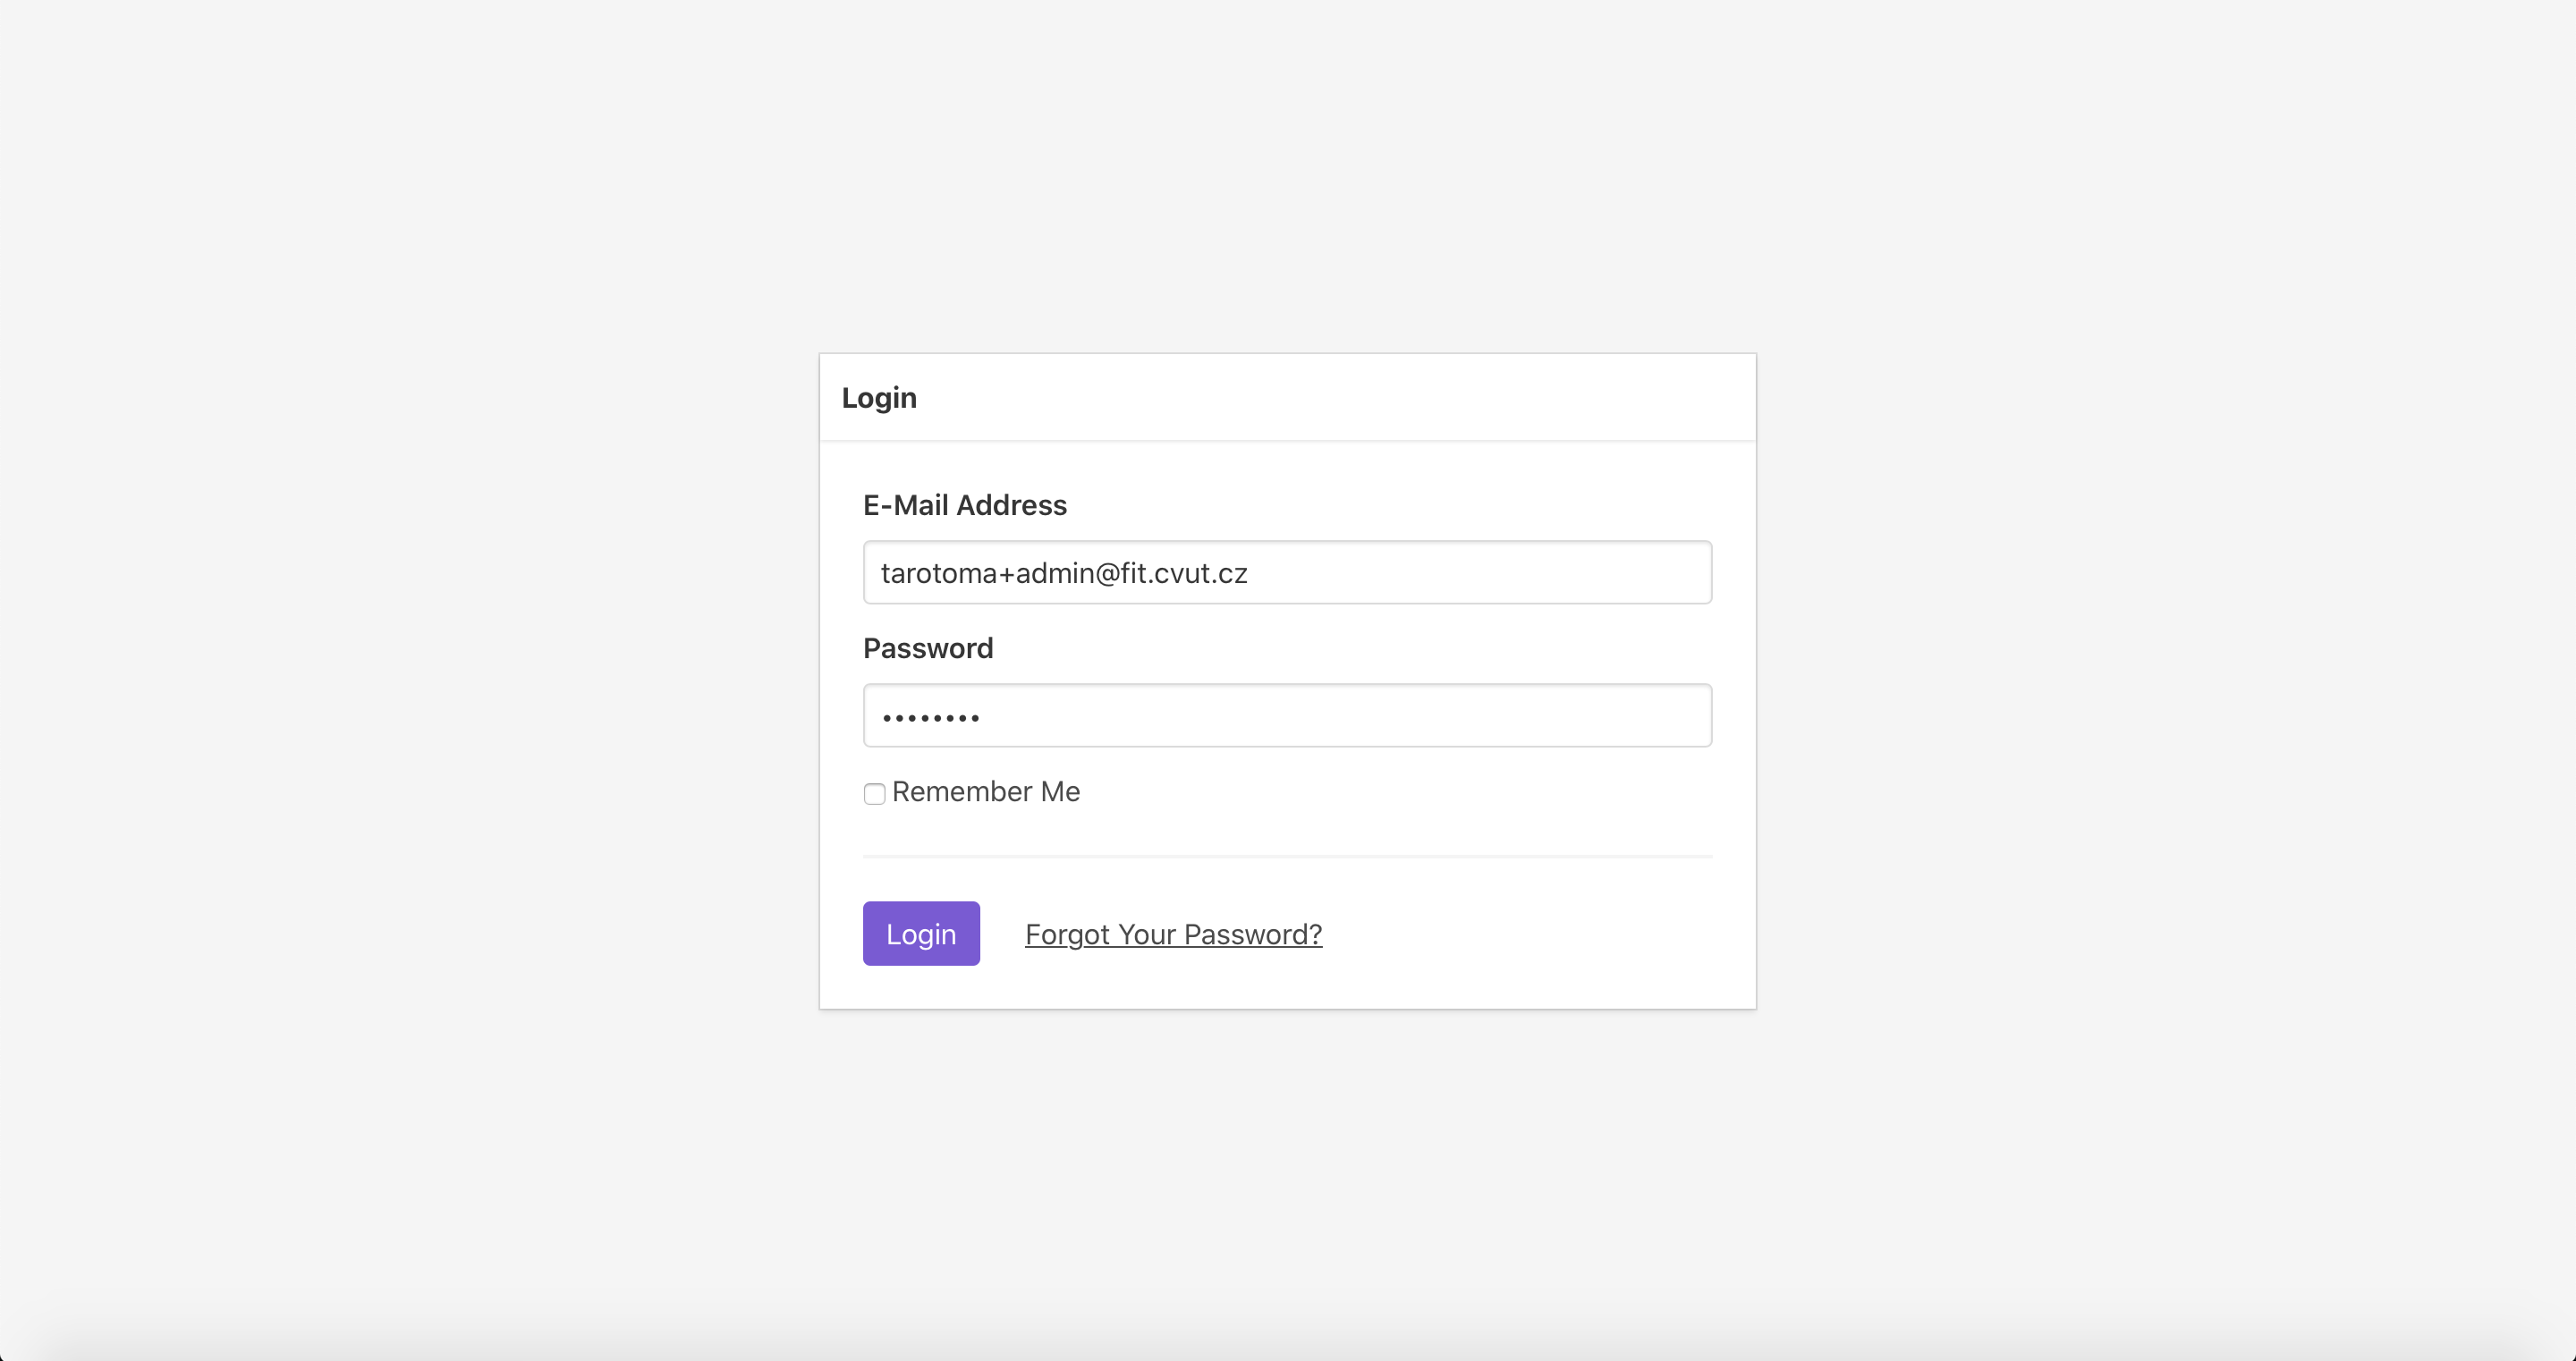
\includegraphics[width=1.0\textwidth]{media/priloha/vseobecne/1.png}
	\caption{Screenshot prihlasovacej obrazovky}
\end{figure}

\begin{figure}[H]
	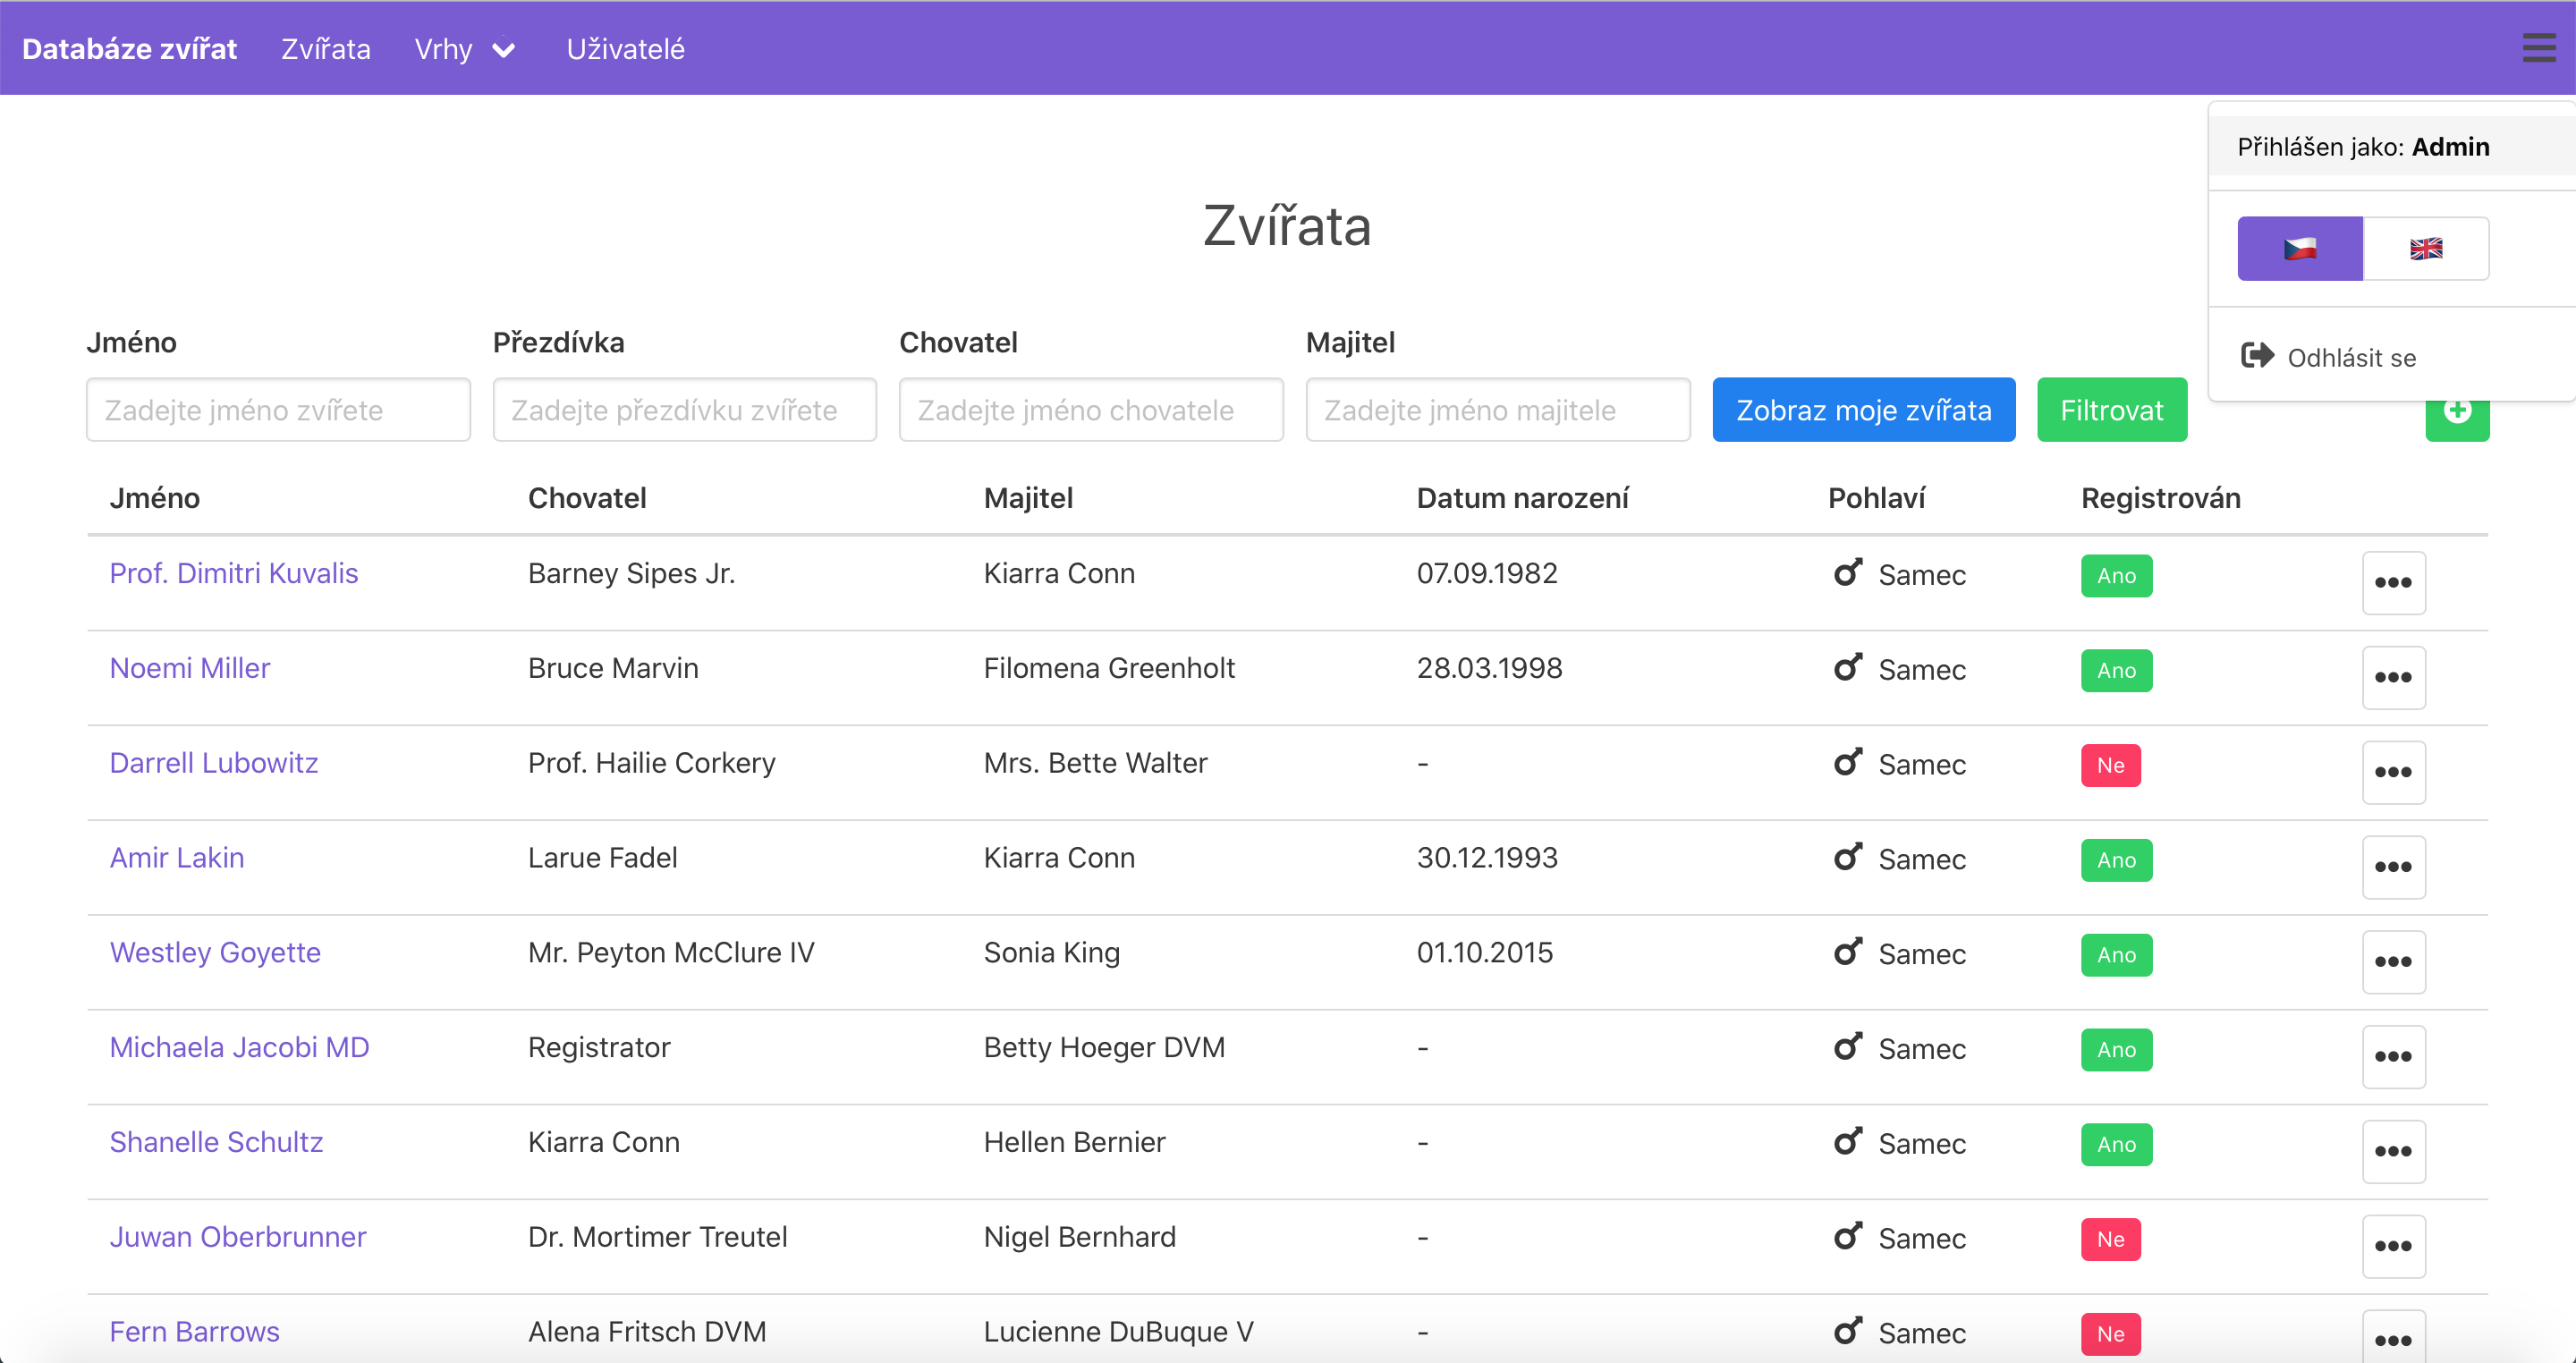
\includegraphics[width=1.0\textwidth]{media/priloha/vseobecne/2.png}
	\caption{Screenshot aplikácie po prihlásení s otvoreným menu}
\end{figure}

\vspace*{\fill}

\begin{figure}[H]
	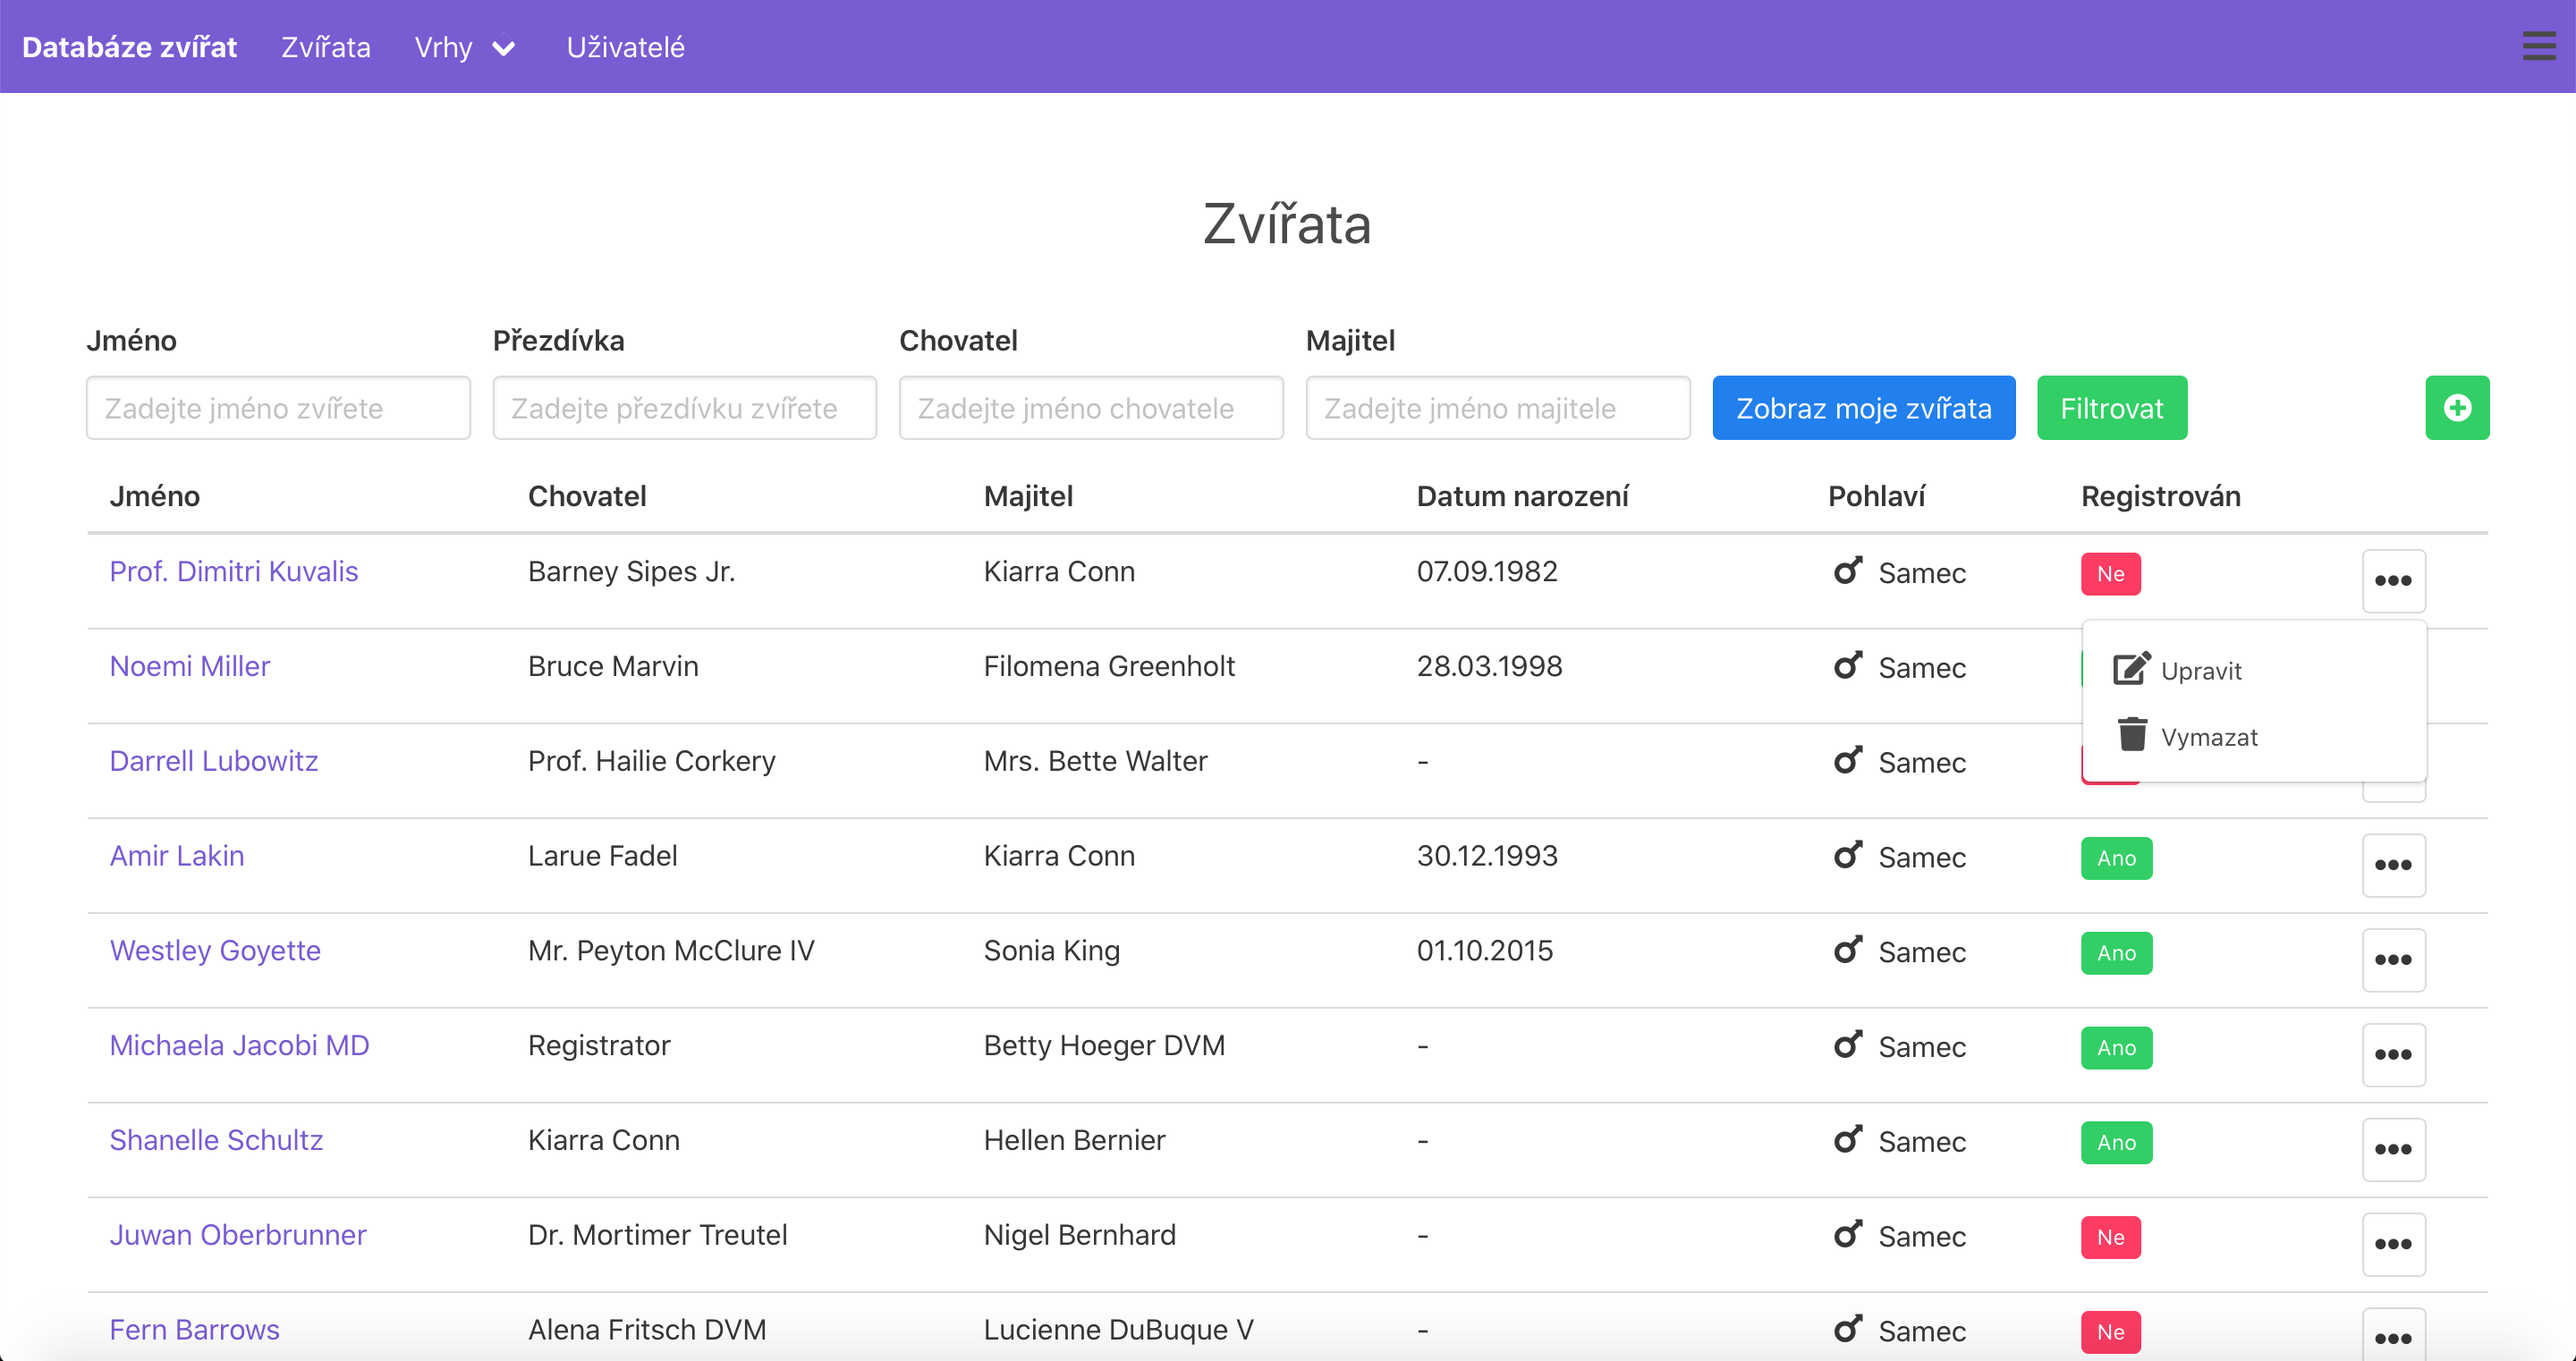
\includegraphics[width=1.0\textwidth]{media/priloha/vseobecne/3.png}
	\caption{Screenshot aplikácie po prihlásení s otvoreným dropdown menu}
\end{figure}

\begin{figure}[H]
	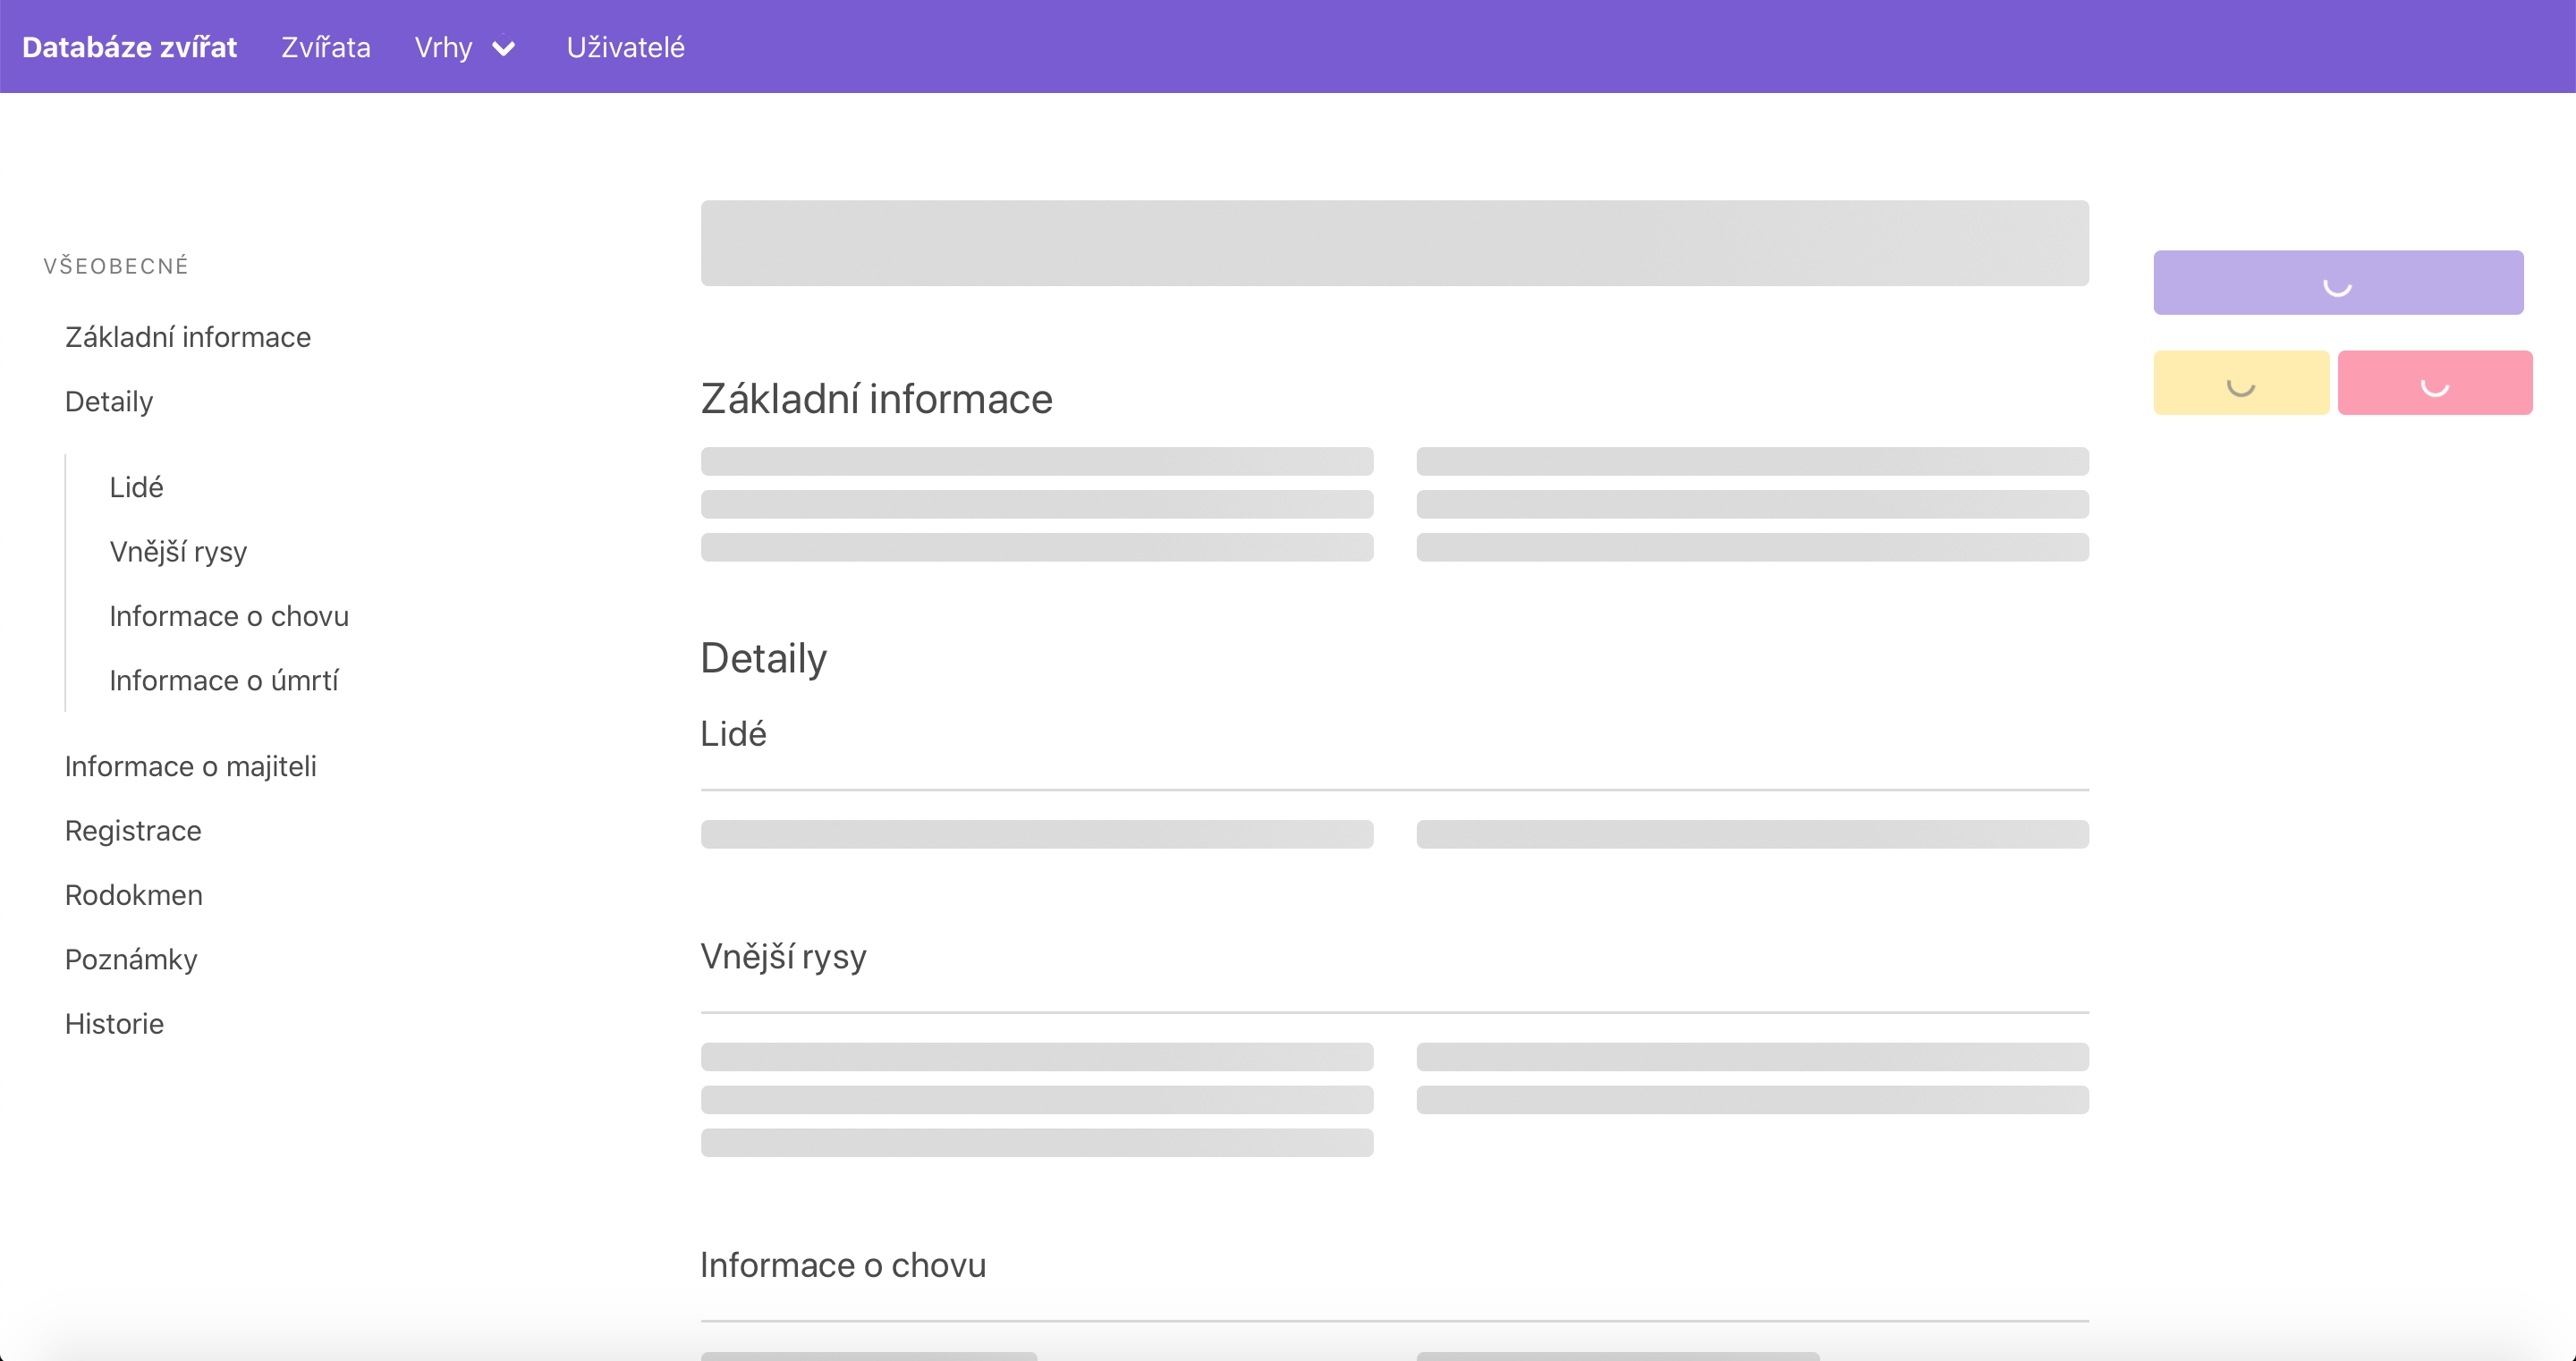
\includegraphics[width=1.0\textwidth]{media/priloha/zviera/1.png}
	\caption{Screenshot načítavania zvoleného zvieraťa}
\end{figure}

\vspace*{\fill}

\begin{figure}[H]
	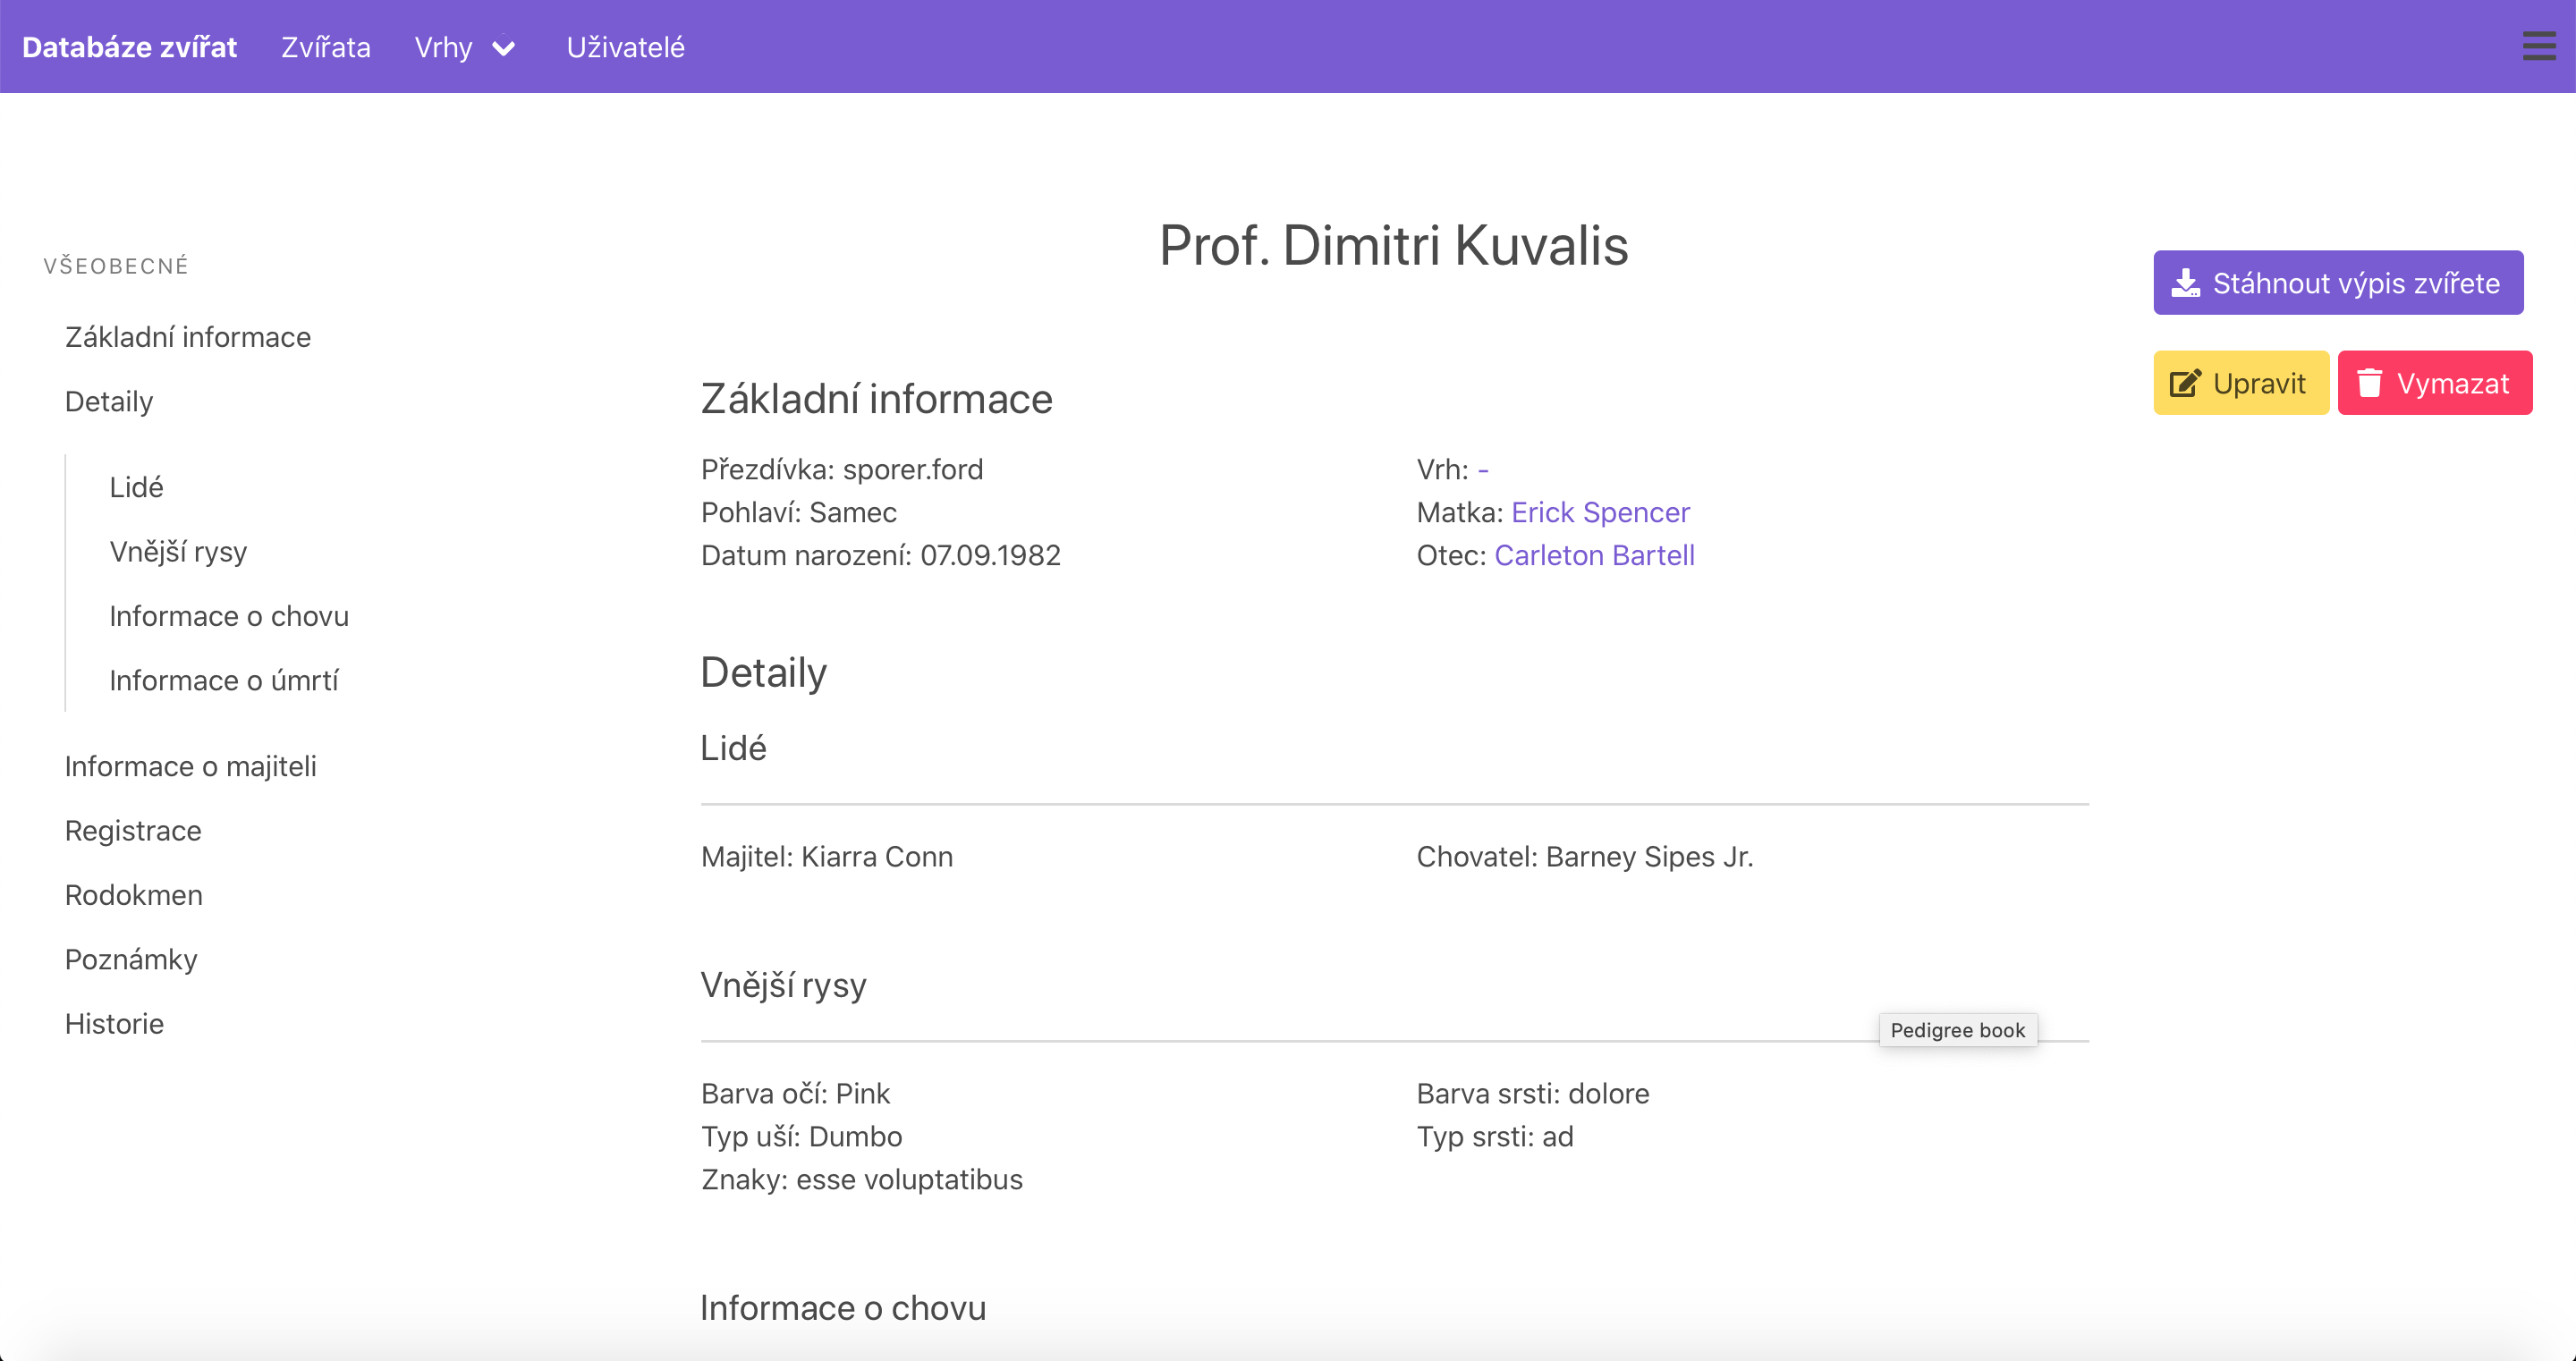
\includegraphics[width=1.0\textwidth]{media/priloha/zviera/2.png}
	\caption{Screenshot načítaného zvoleného zvieraťa}
\end{figure}

\begin{figure}[H]
	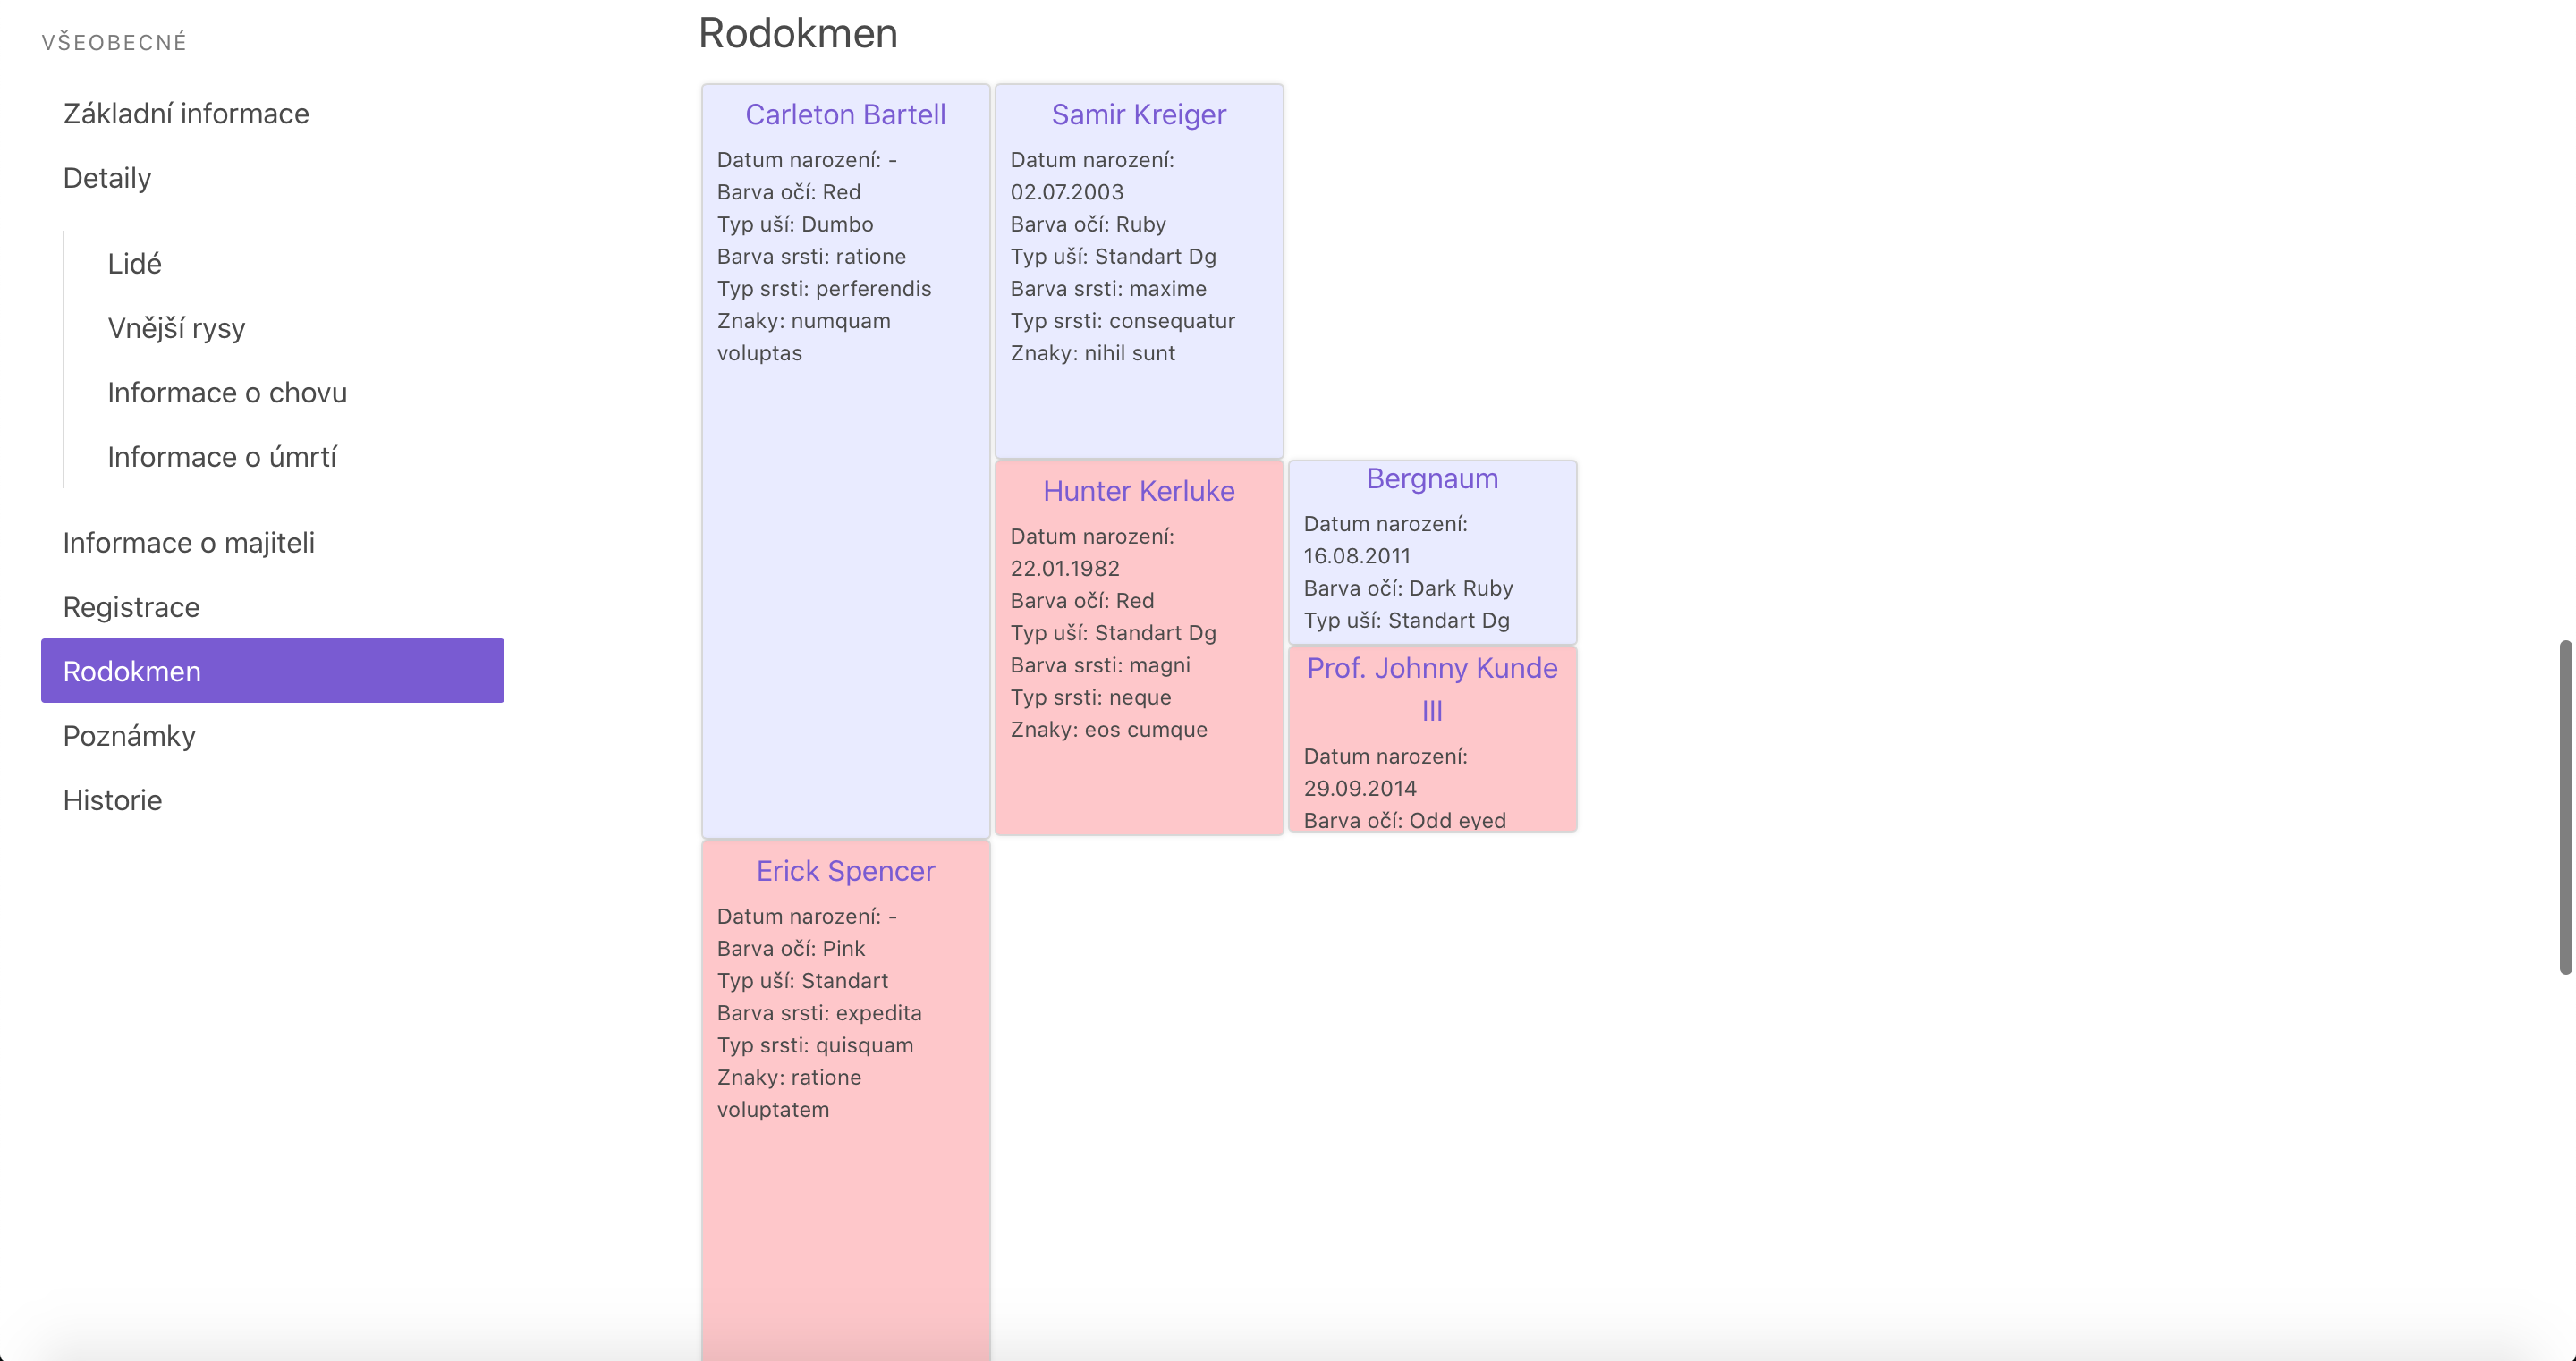
\includegraphics[width=1.0\textwidth]{media/priloha/zviera/3.png}
	\caption{Screenshot zobrazenia rodokmeňu zvoleného zvieraťa}
\end{figure}

\vspace*{\fill}

\begin{figure}[H]
	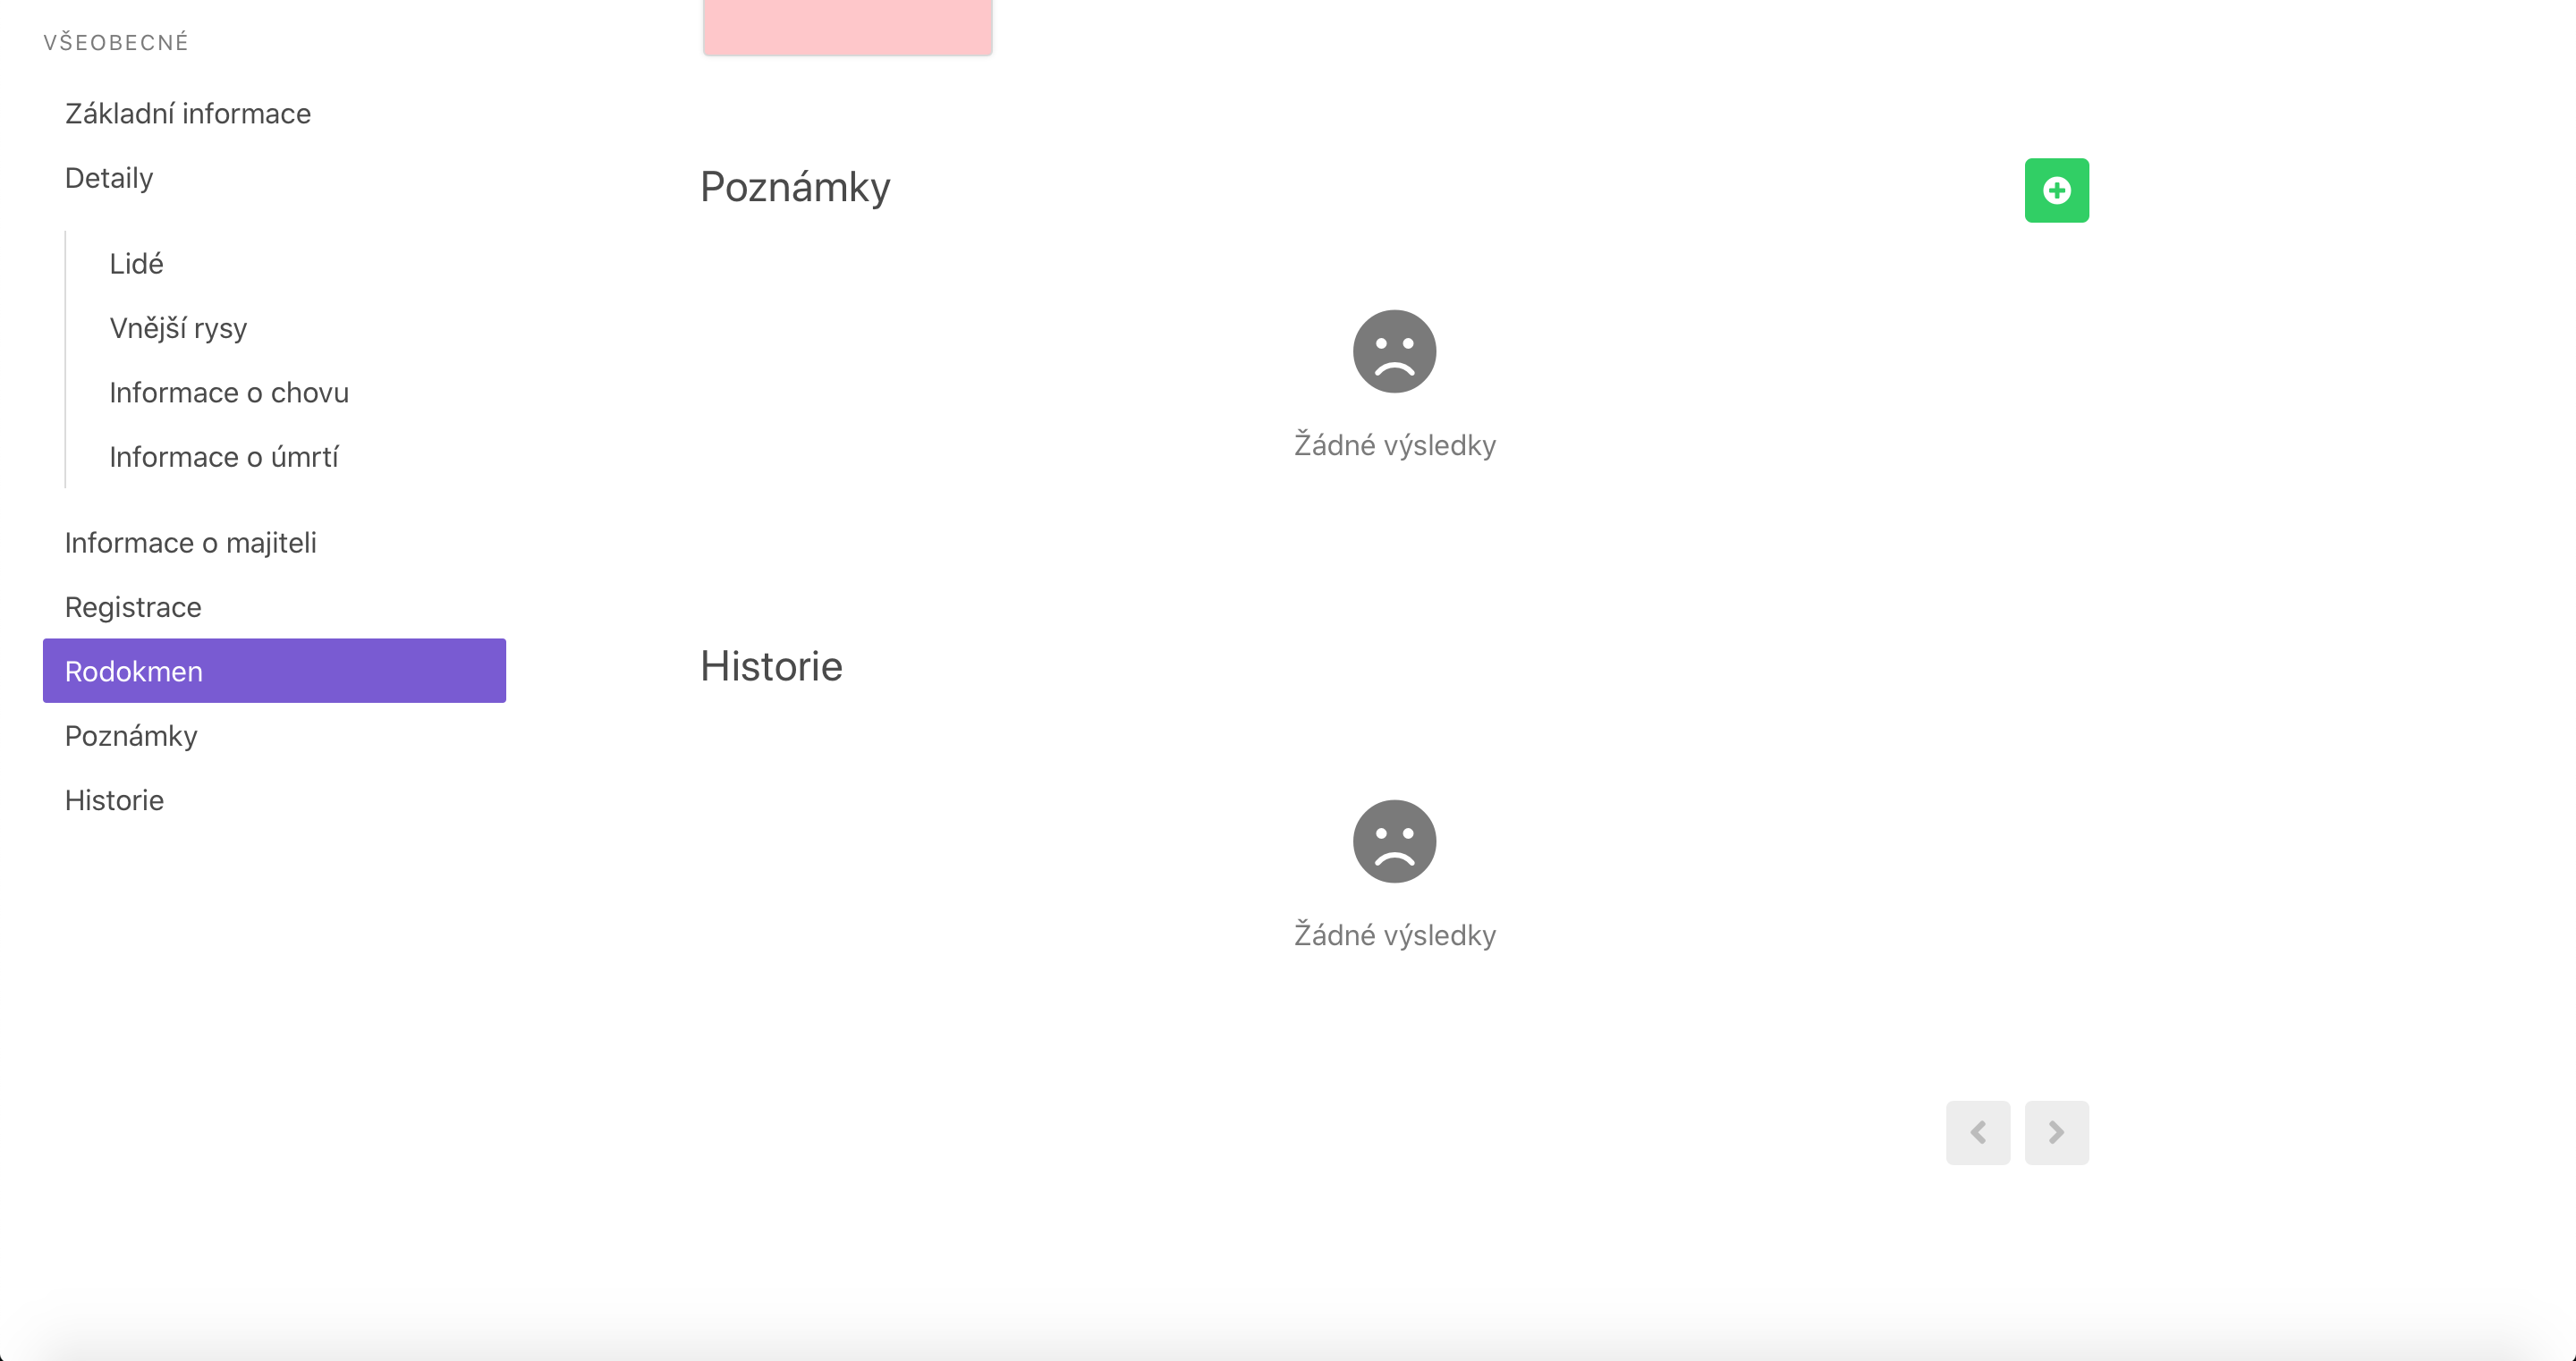
\includegraphics[width=1.0\textwidth]{media/priloha/zviera/4.png}
	\caption{Screenshot zobrazenia poznámok a histórie zvoleného zvieraťa}
\end{figure}

\begin{figure}[H]
	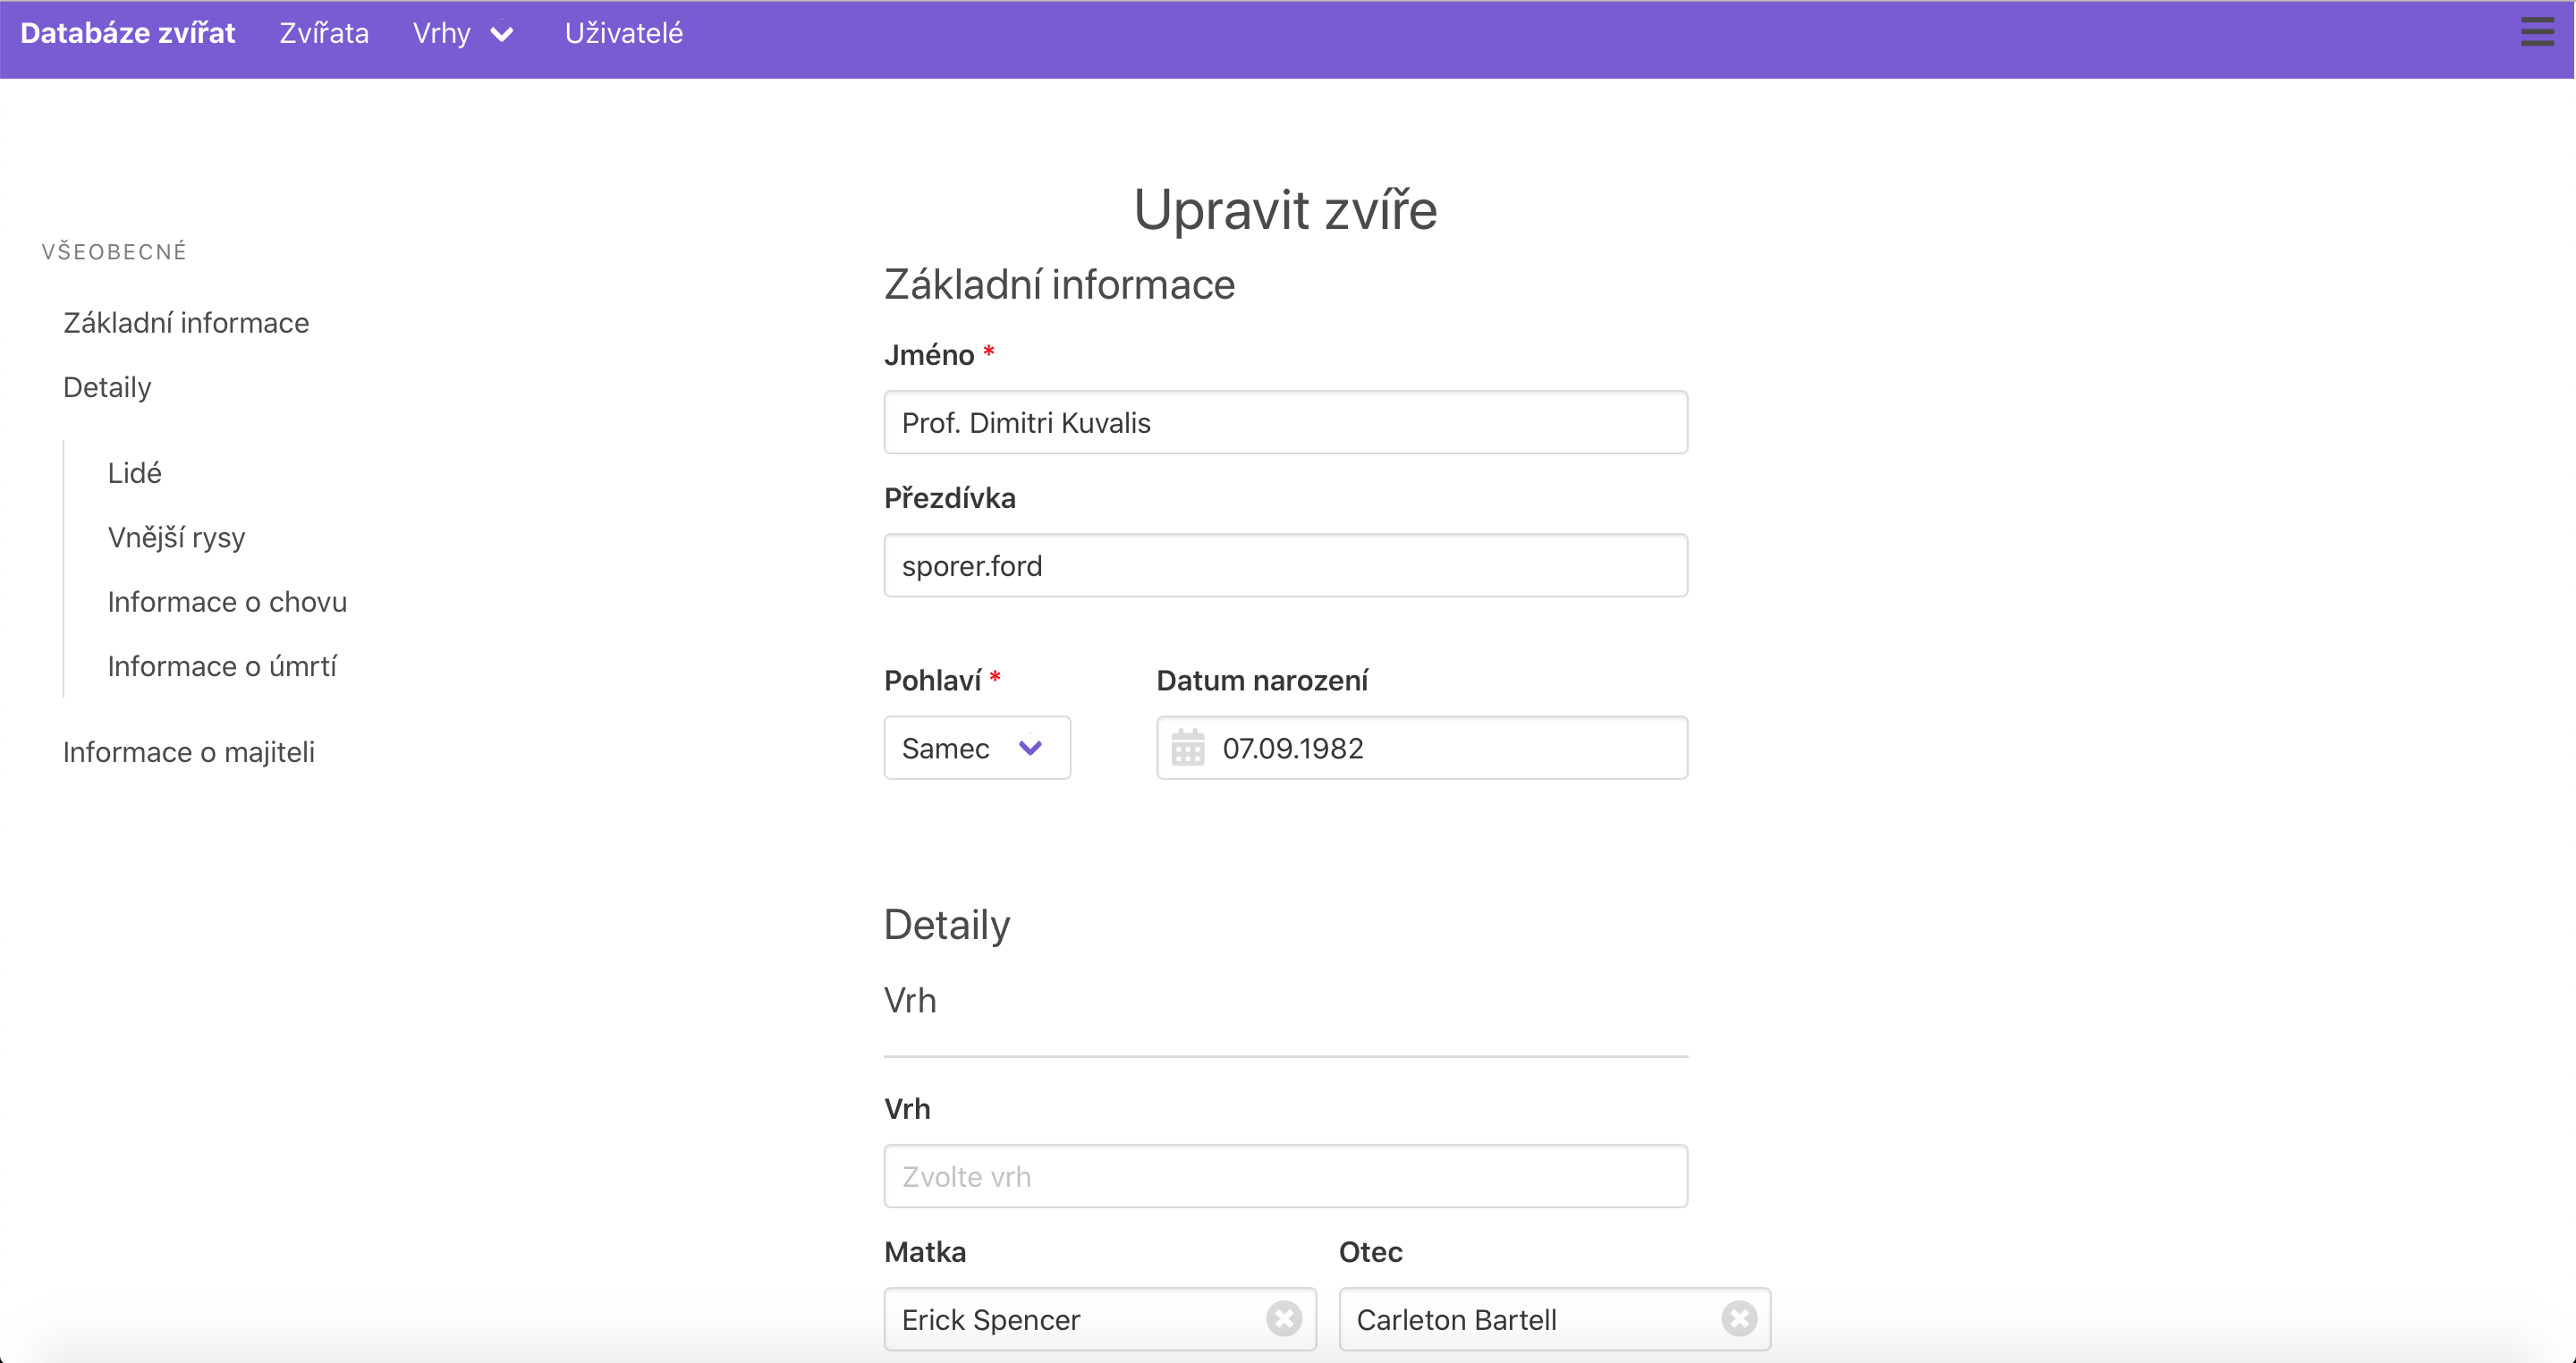
\includegraphics[width=1.0\textwidth]{media/priloha/zviera/editacia/1.png}
	\caption{Screenshot zobrazenia sekcie editácie zvieraťa}
\end{figure}

\vspace*{\fill}

\begin{figure}[H]
	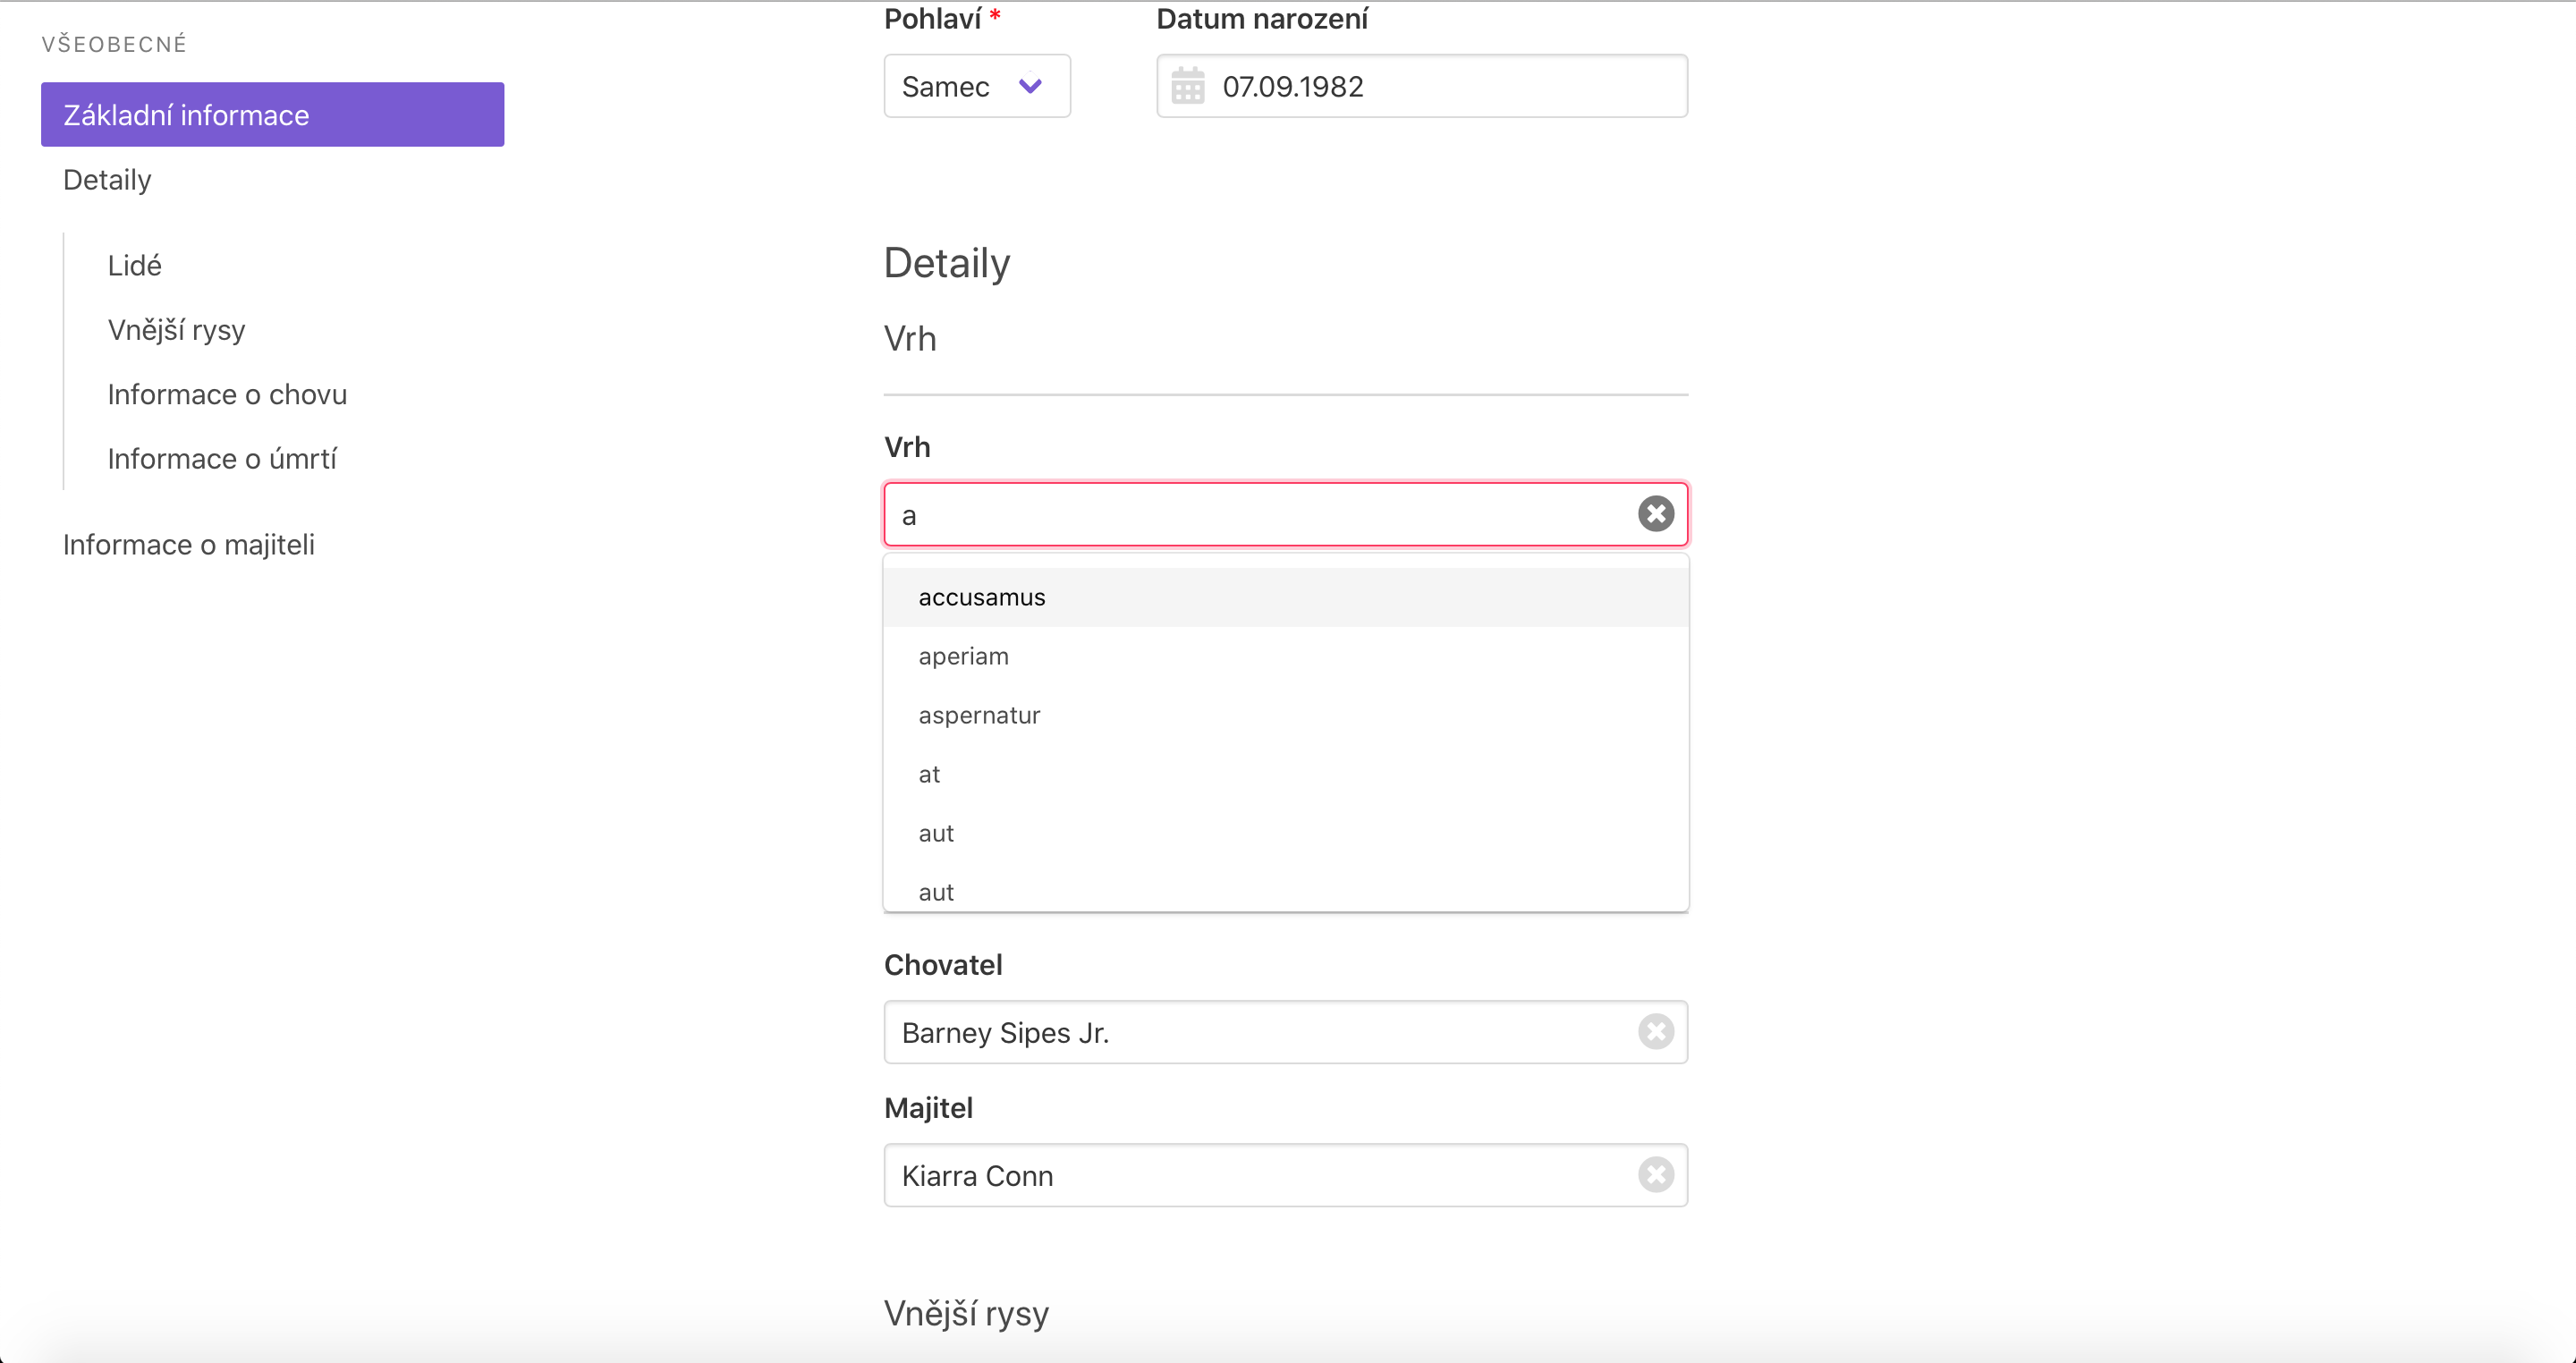
\includegraphics[width=1.0\textwidth]{media/priloha/zviera/editacia/2.png}
	\caption{Screenshot zobrazenia ponuky voľby vrhu pri editácii zvieraťa}
\end{figure}

\begin{figure}[H]
	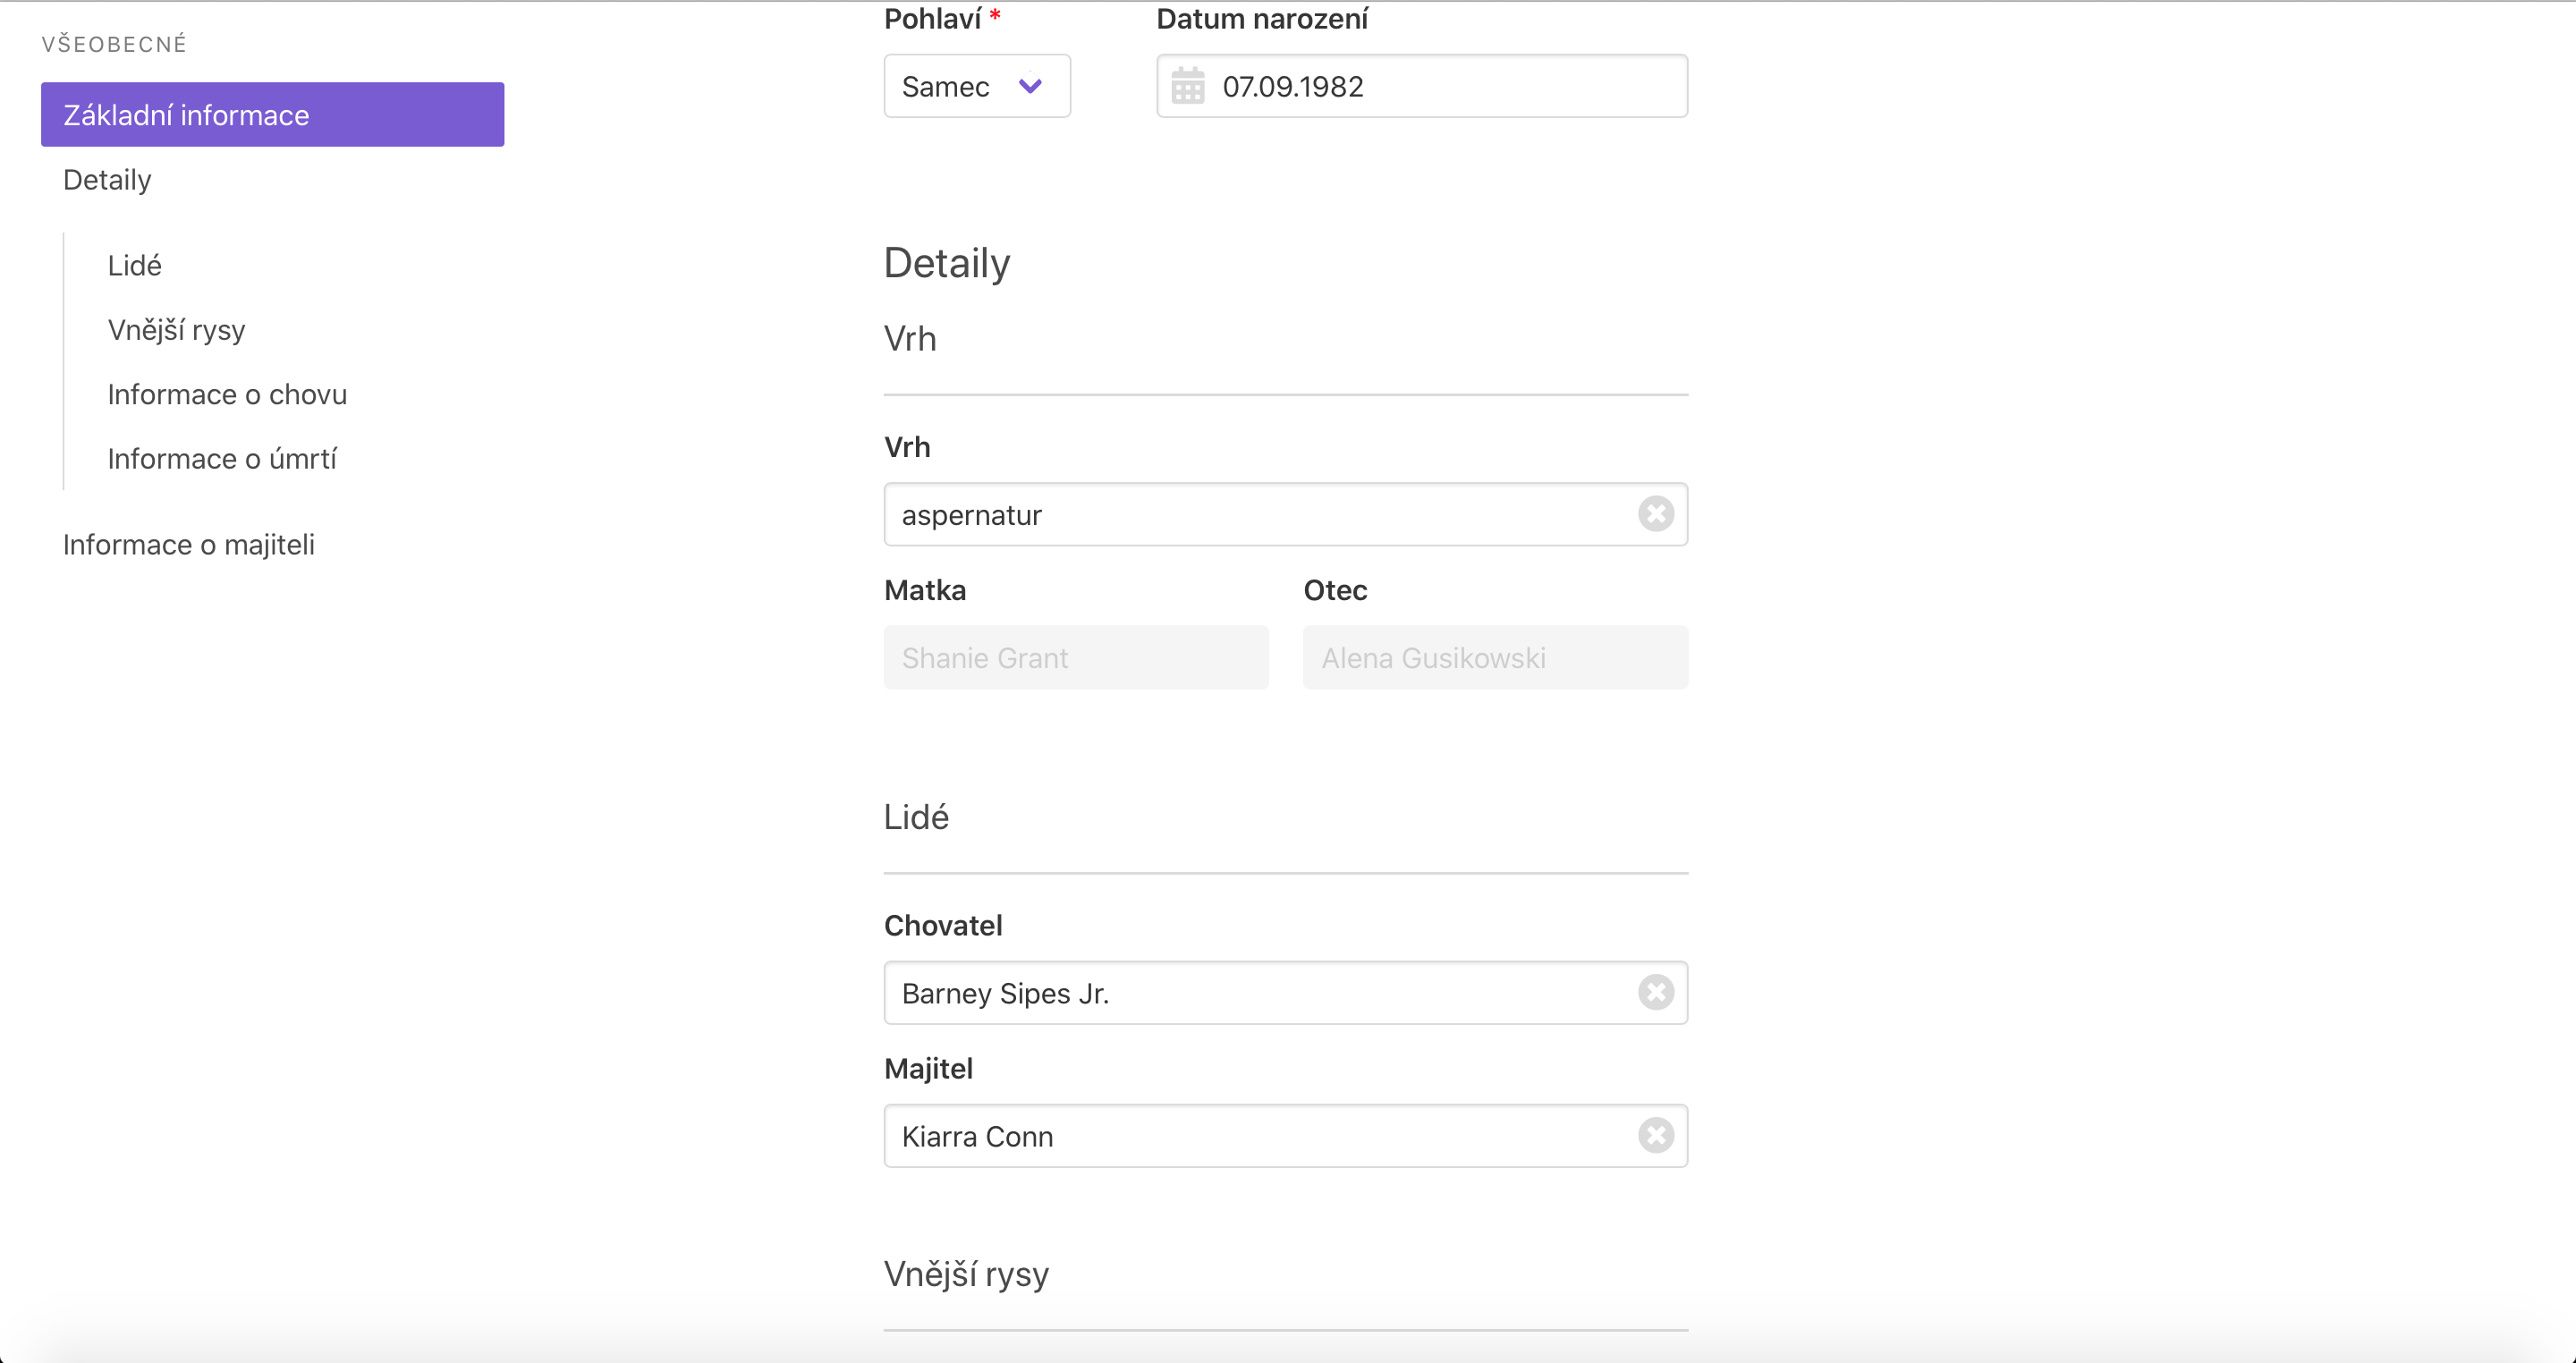
\includegraphics[width=1.0\textwidth]{media/priloha/zviera/editacia/3.png}
	\caption{Screenshot aplikácie po zvolení vrhu pri editácii zvieraťa}
\end{figure}

\vspace*{\fill}

\begin{figure}[H]
	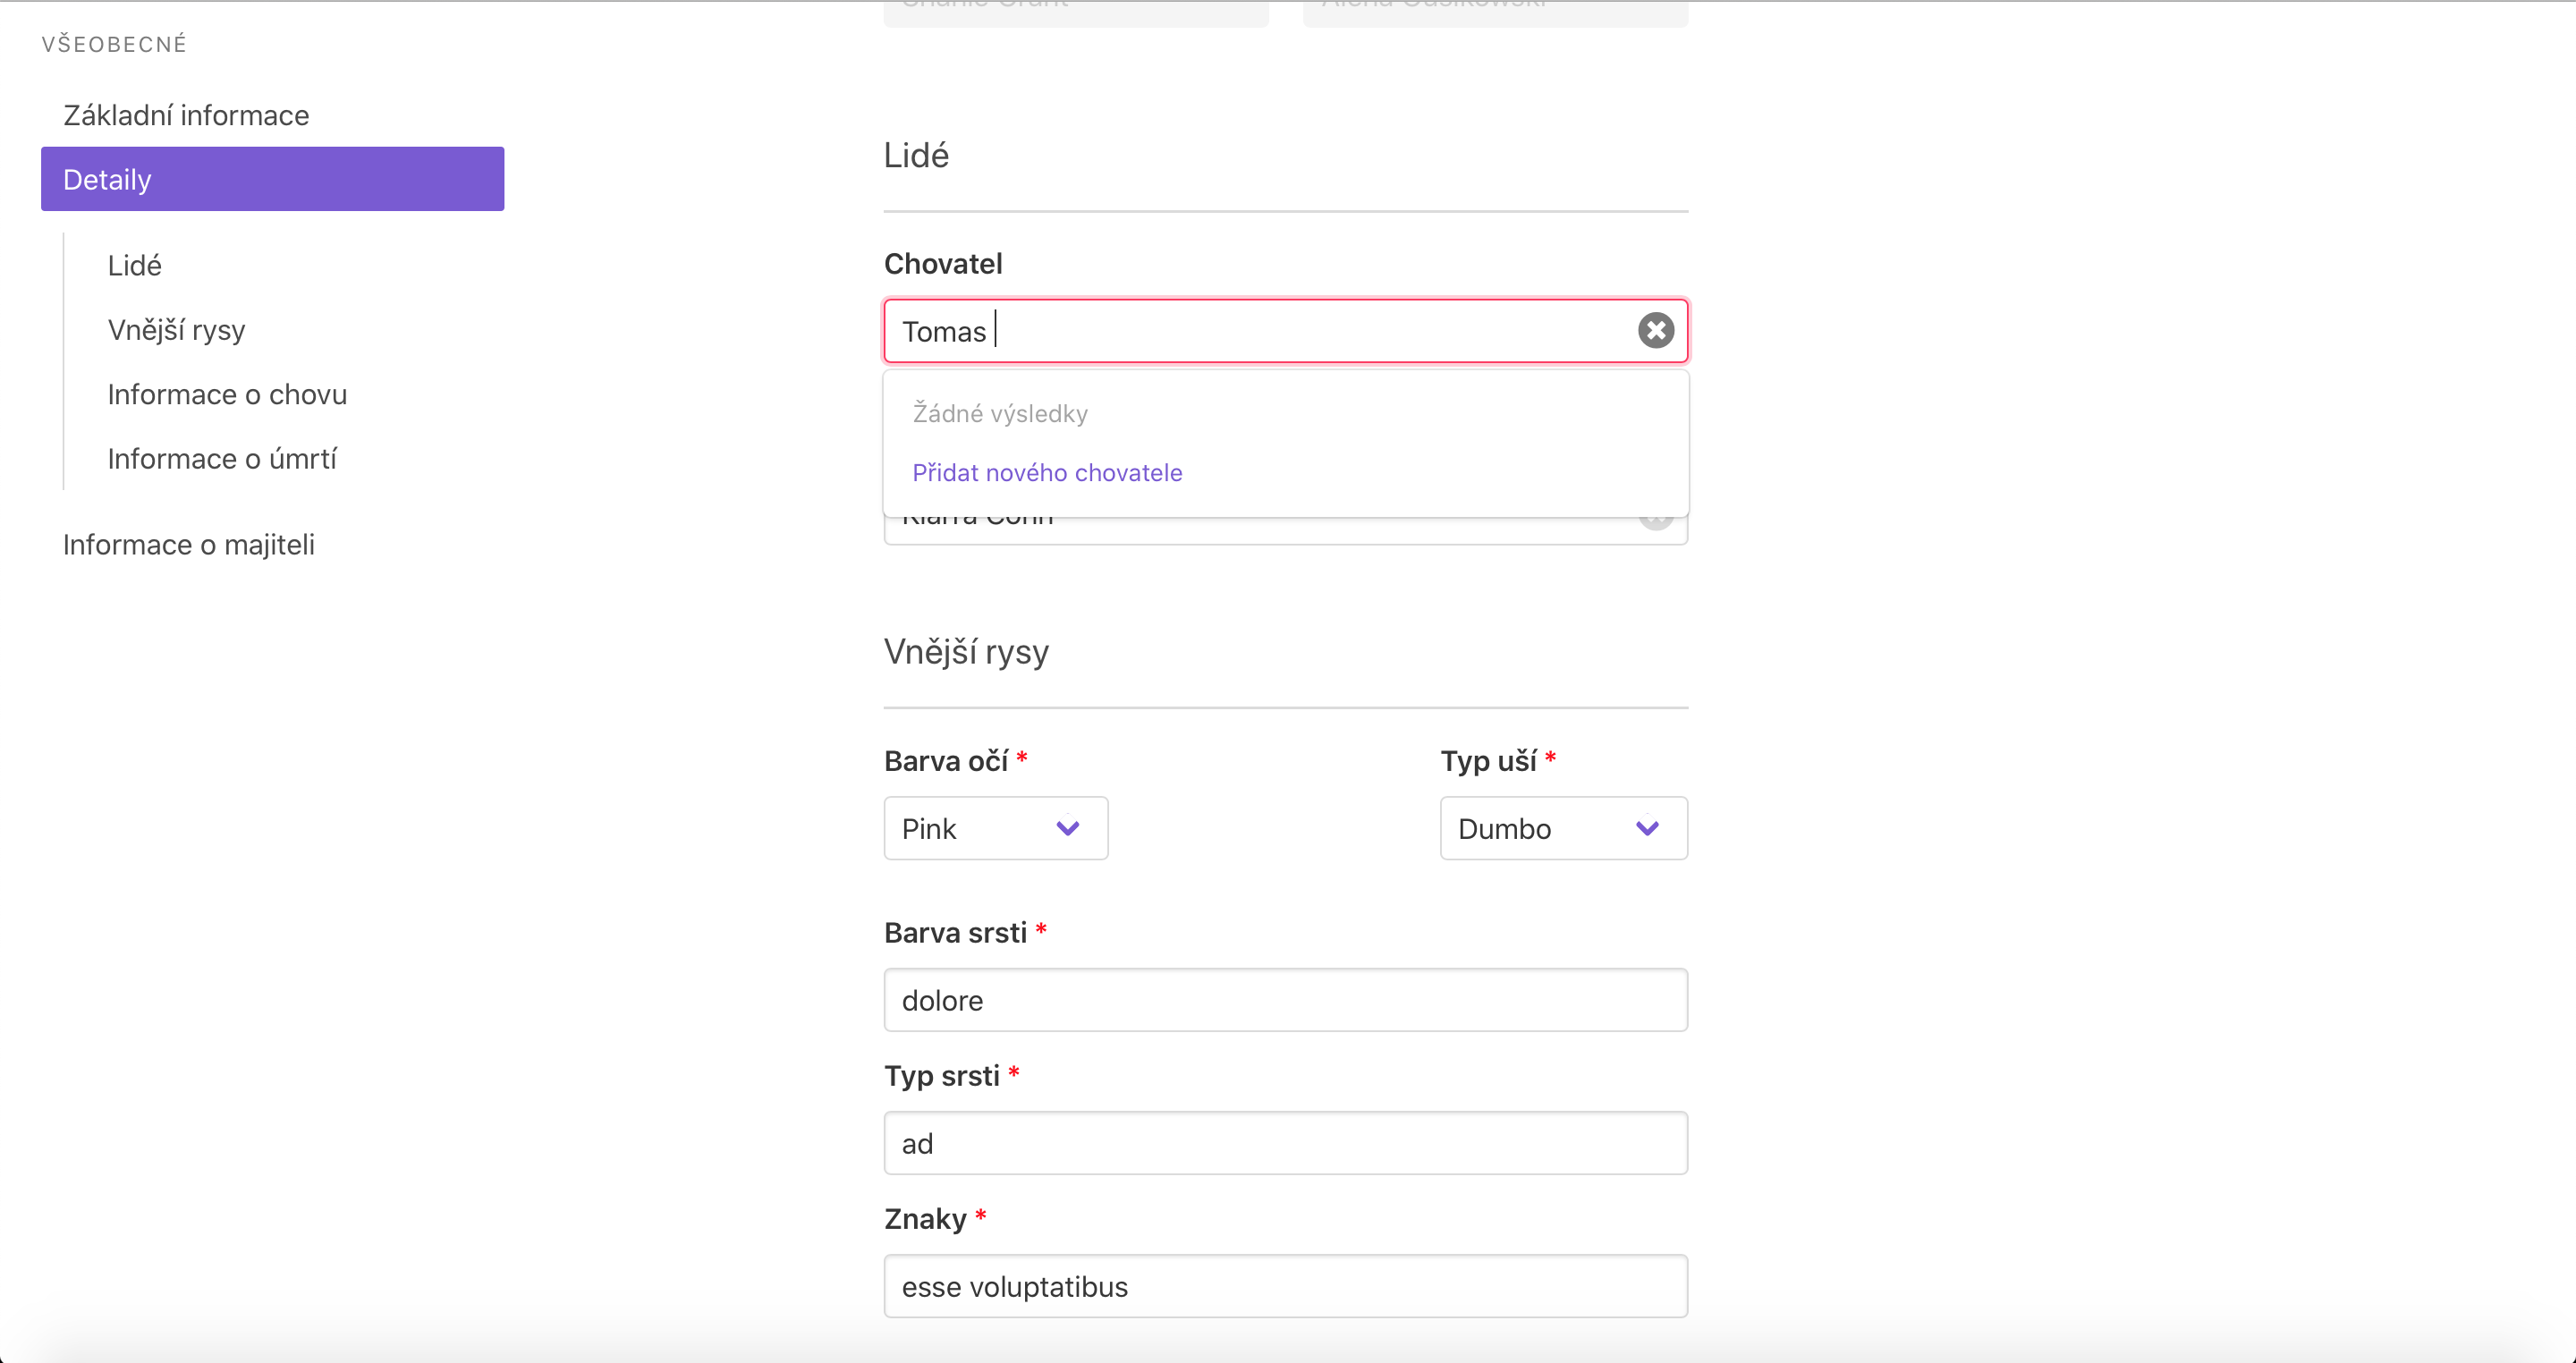
\includegraphics[width=1.0\textwidth]{media/priloha/zviera/editacia/4.png}
	\caption{Screenshot aplikácie zobrazujúci možnosť voľby chovateľa}
\end{figure}

\begin{figure}[H]
	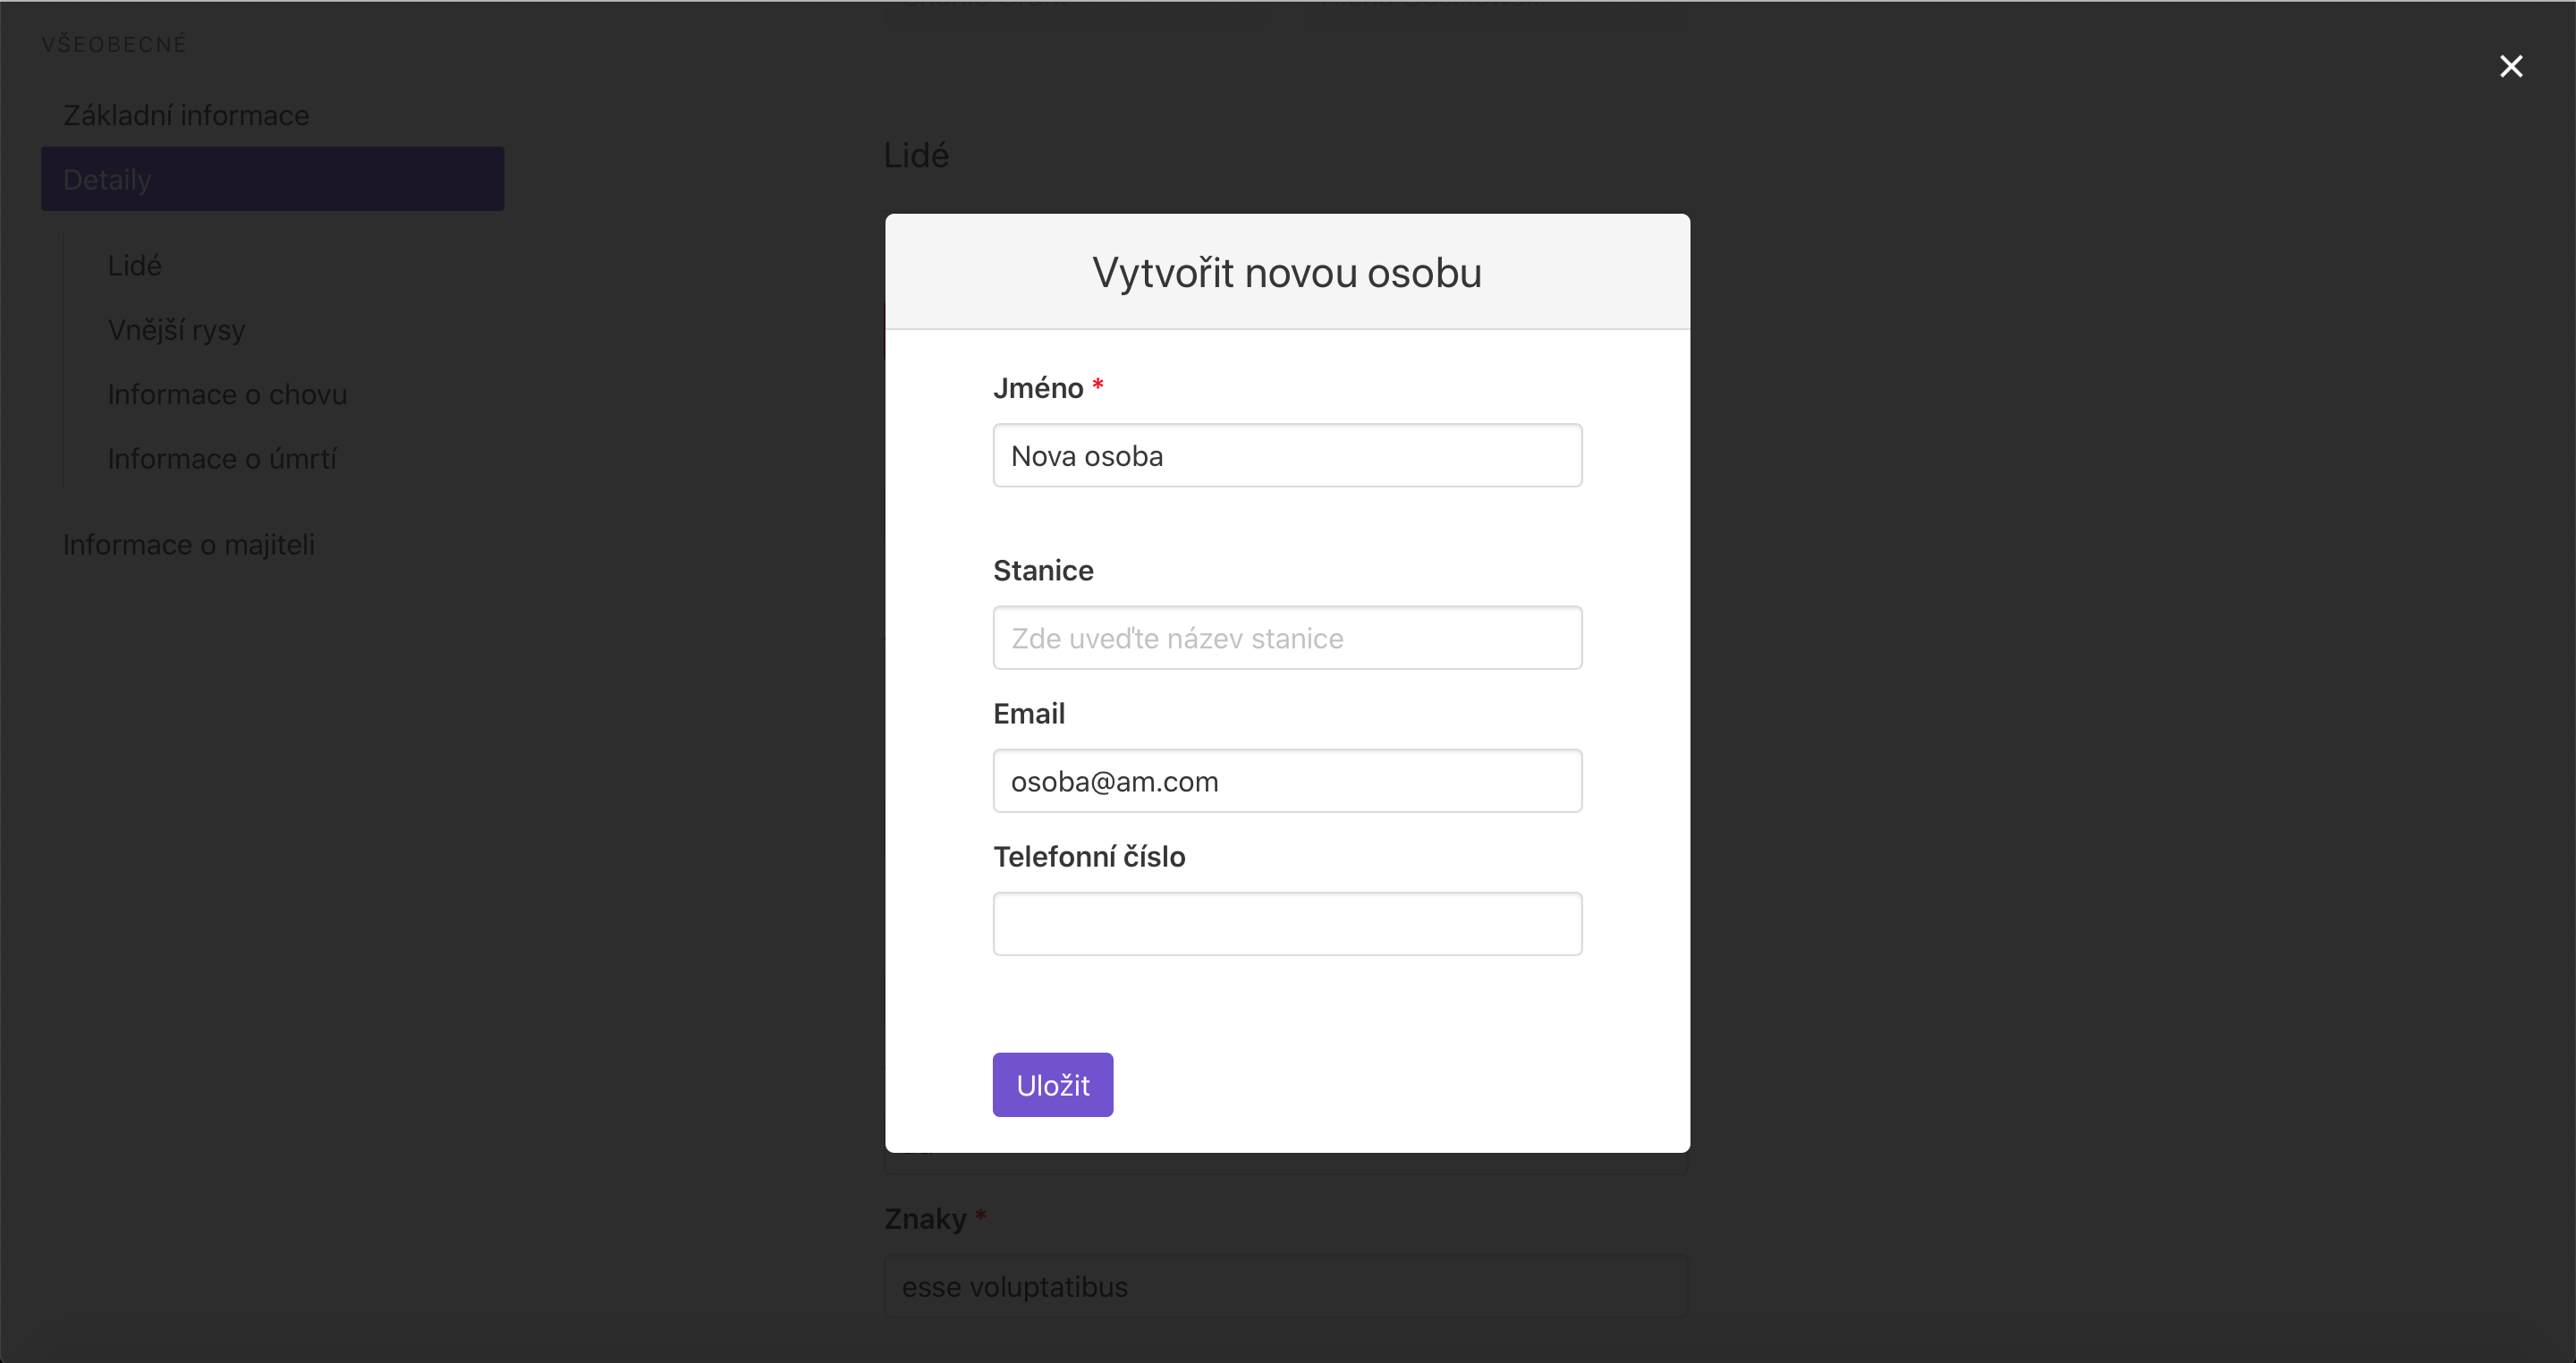
\includegraphics[width=1.0\textwidth]{media/priloha/zviera/editacia/5.png}
	\caption{Screenshot modálneho okna s ponukou vytvorenia novej osoby}
\end{figure}

\vspace*{\fill}

\begin{figure}[H]
	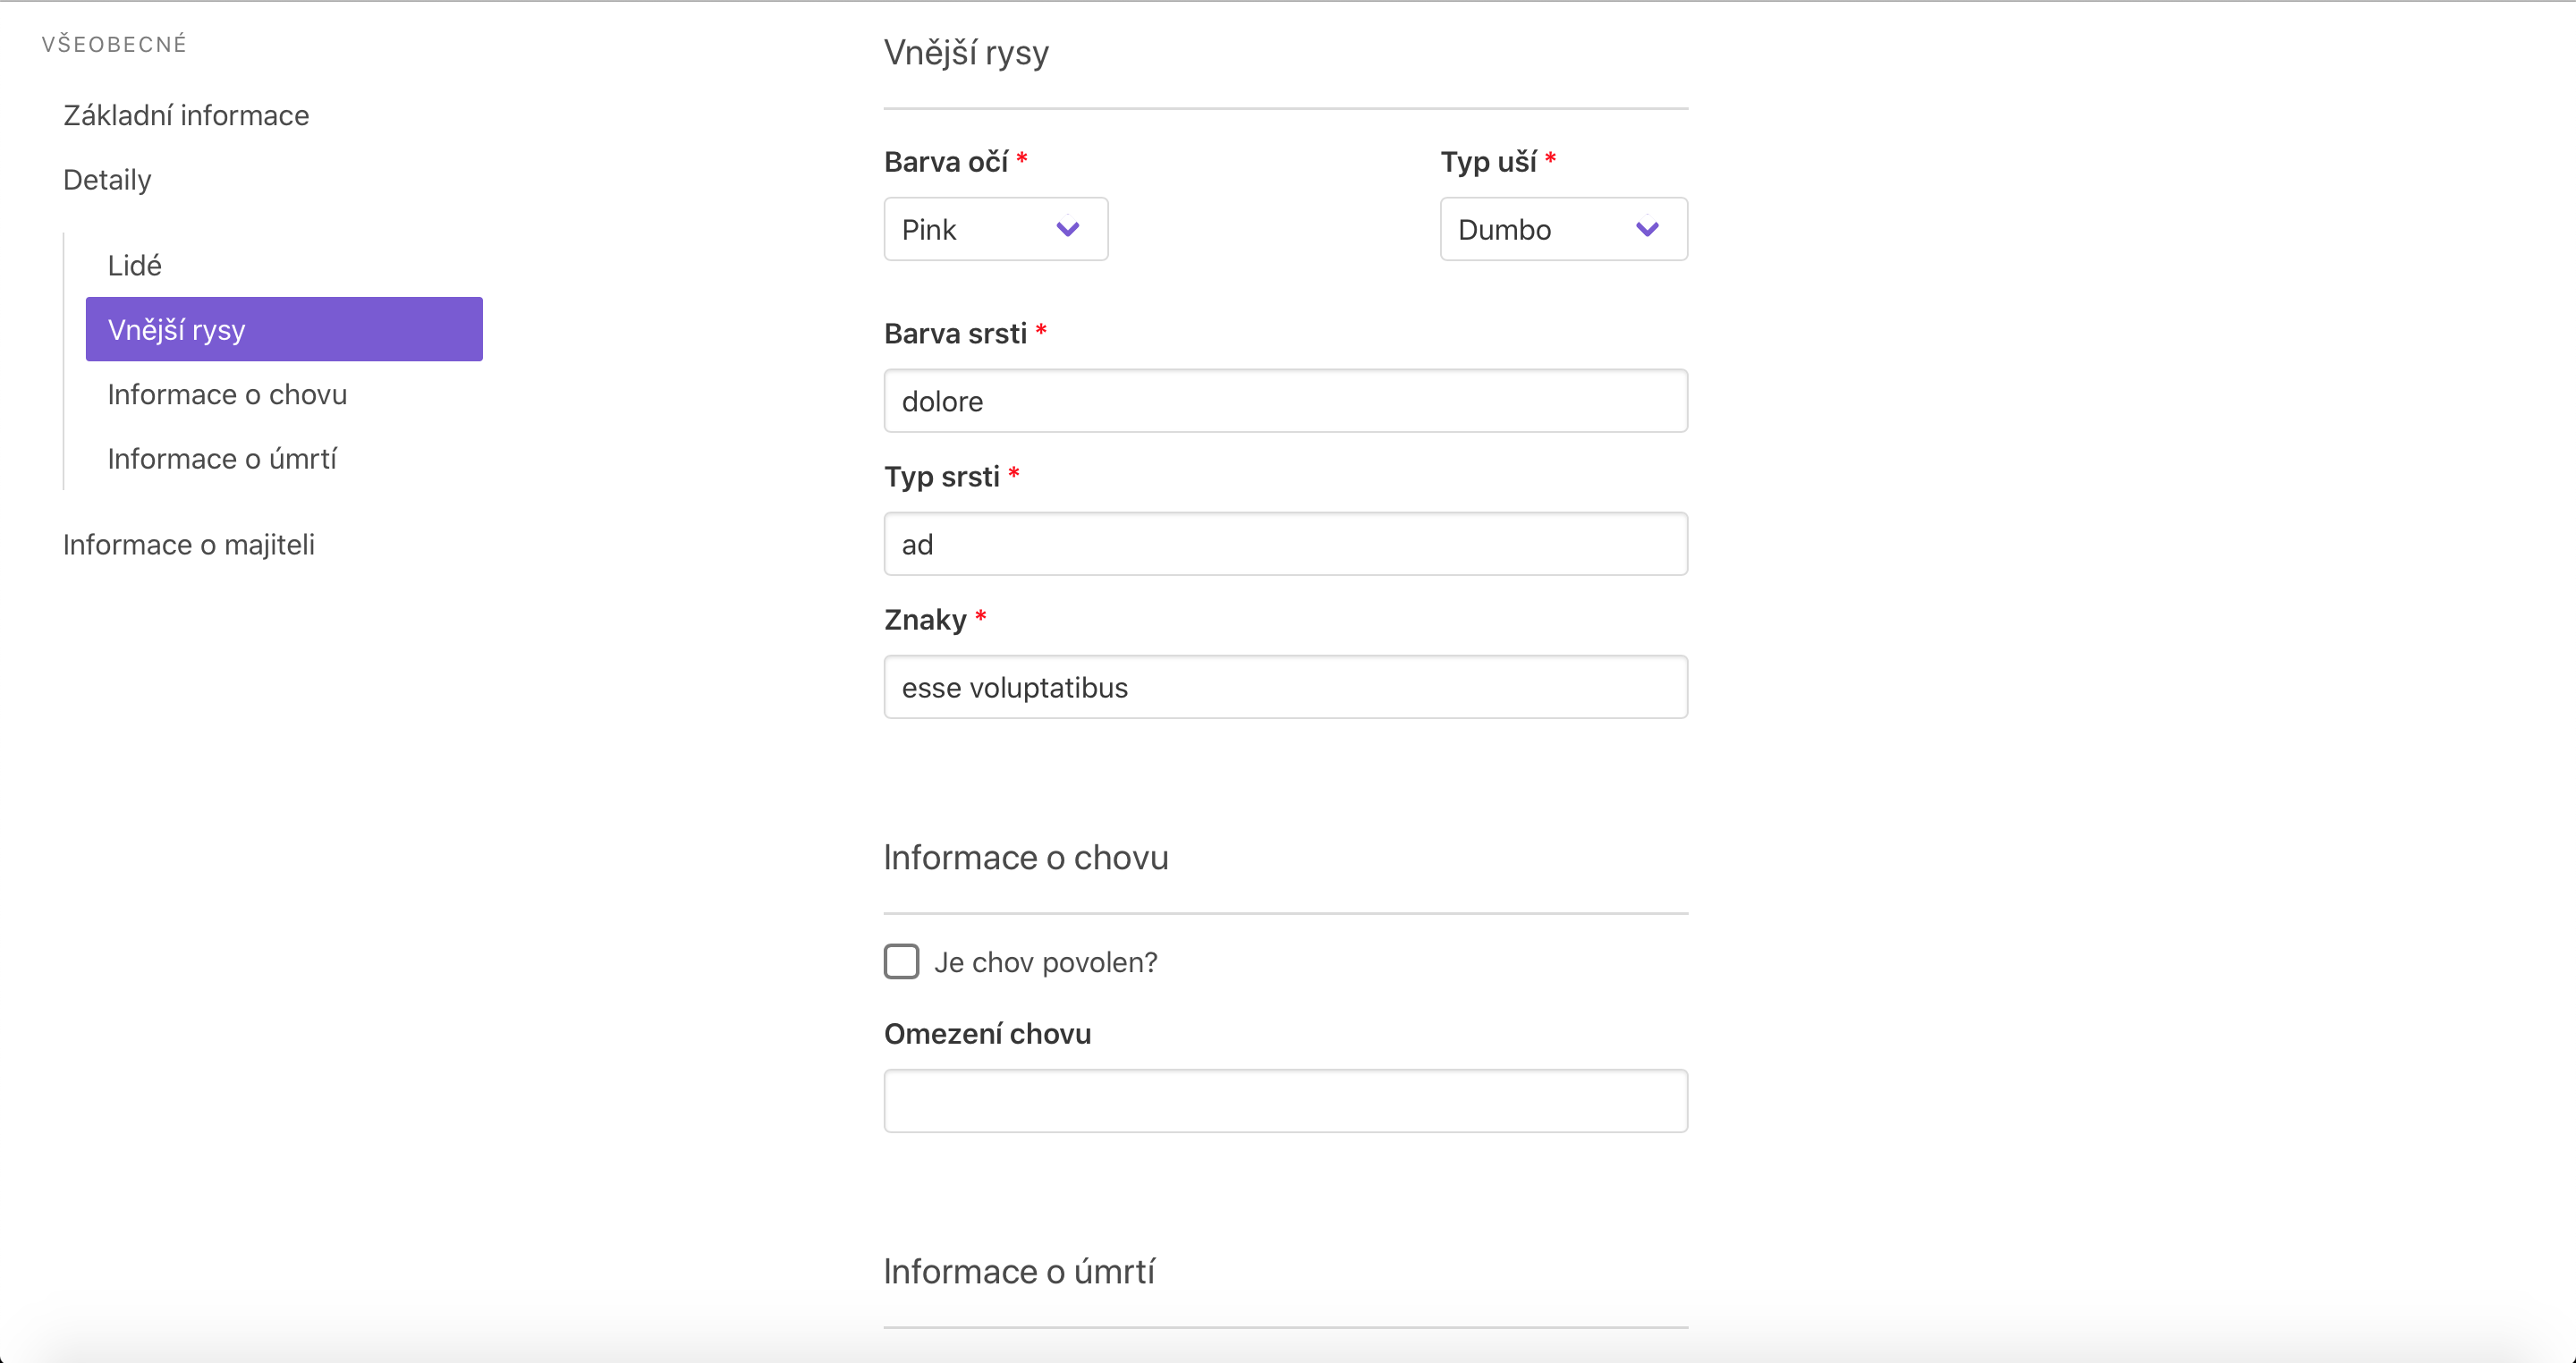
\includegraphics[width=1.0\textwidth]{media/priloha/zviera/editacia/6.png}
	\caption{Screenshot zobrazenia nasledujúcej sekcie pri editácii zvieraťa}
\end{figure}

\begin{figure}[H]
	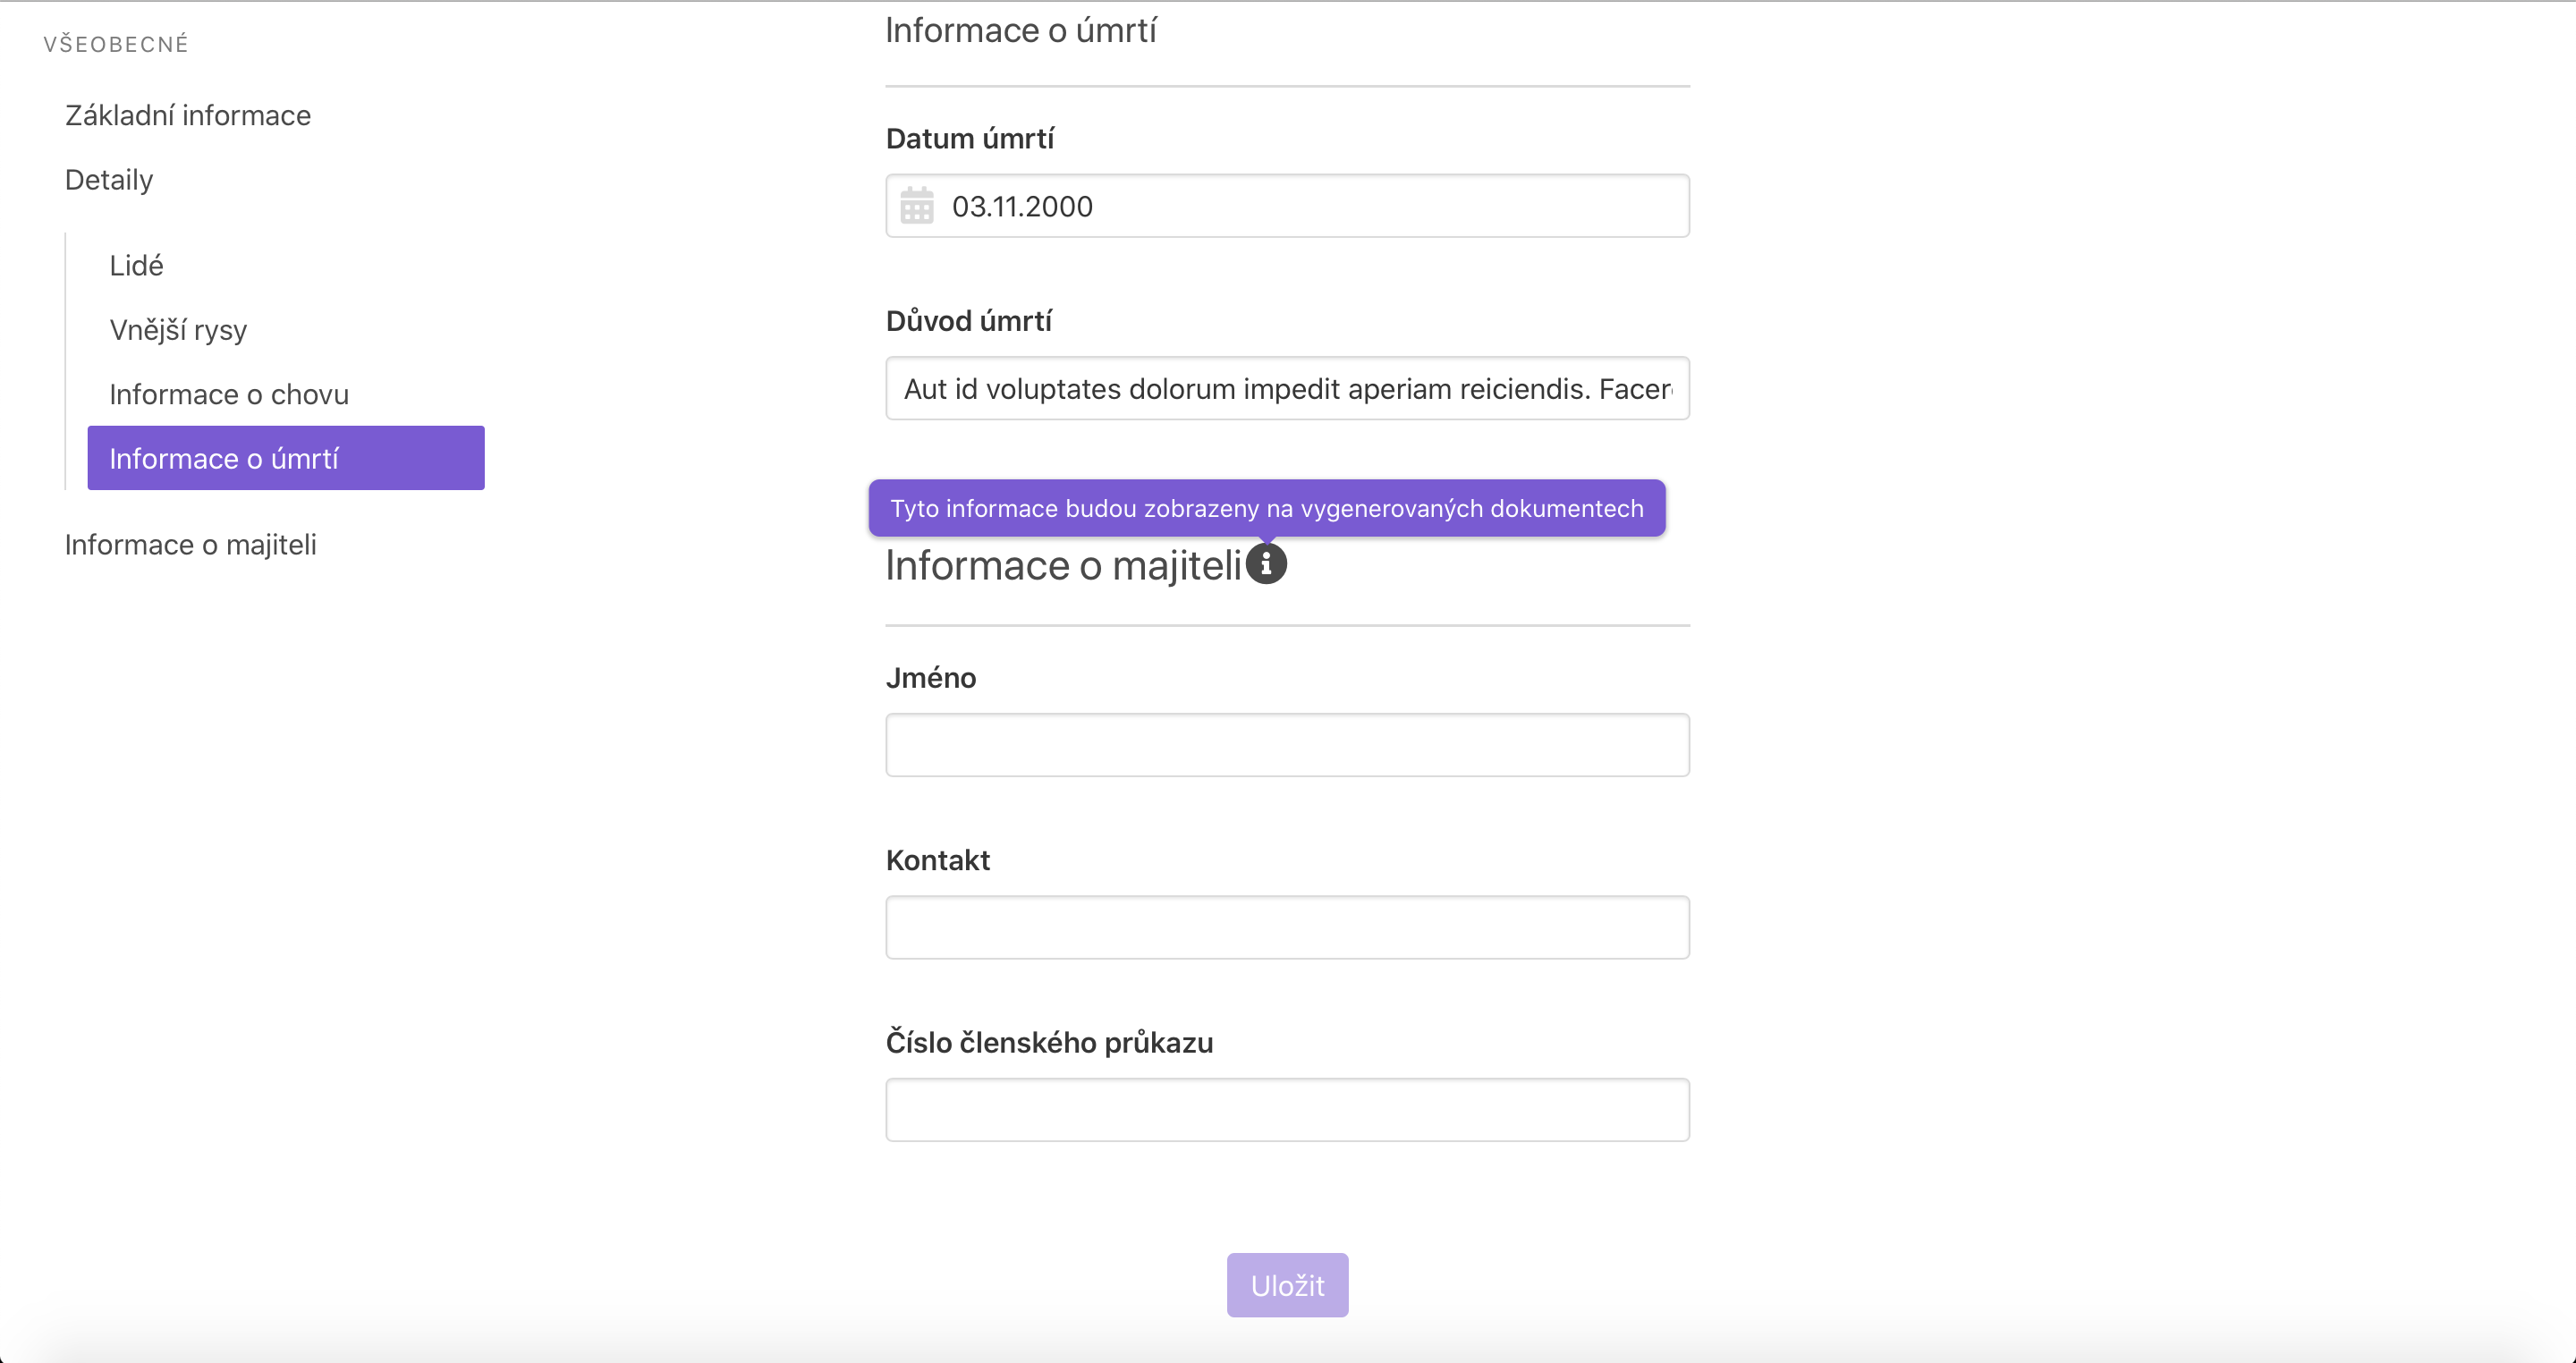
\includegraphics[width=1.0\textwidth]{media/priloha/zviera/editacia/7.png}
	\caption{Screenshot zobrazenia poslednej sekcie pri editácii zvieraťa}
\end{figure}

\vspace*{\fill}

\begin{figure}[H]
	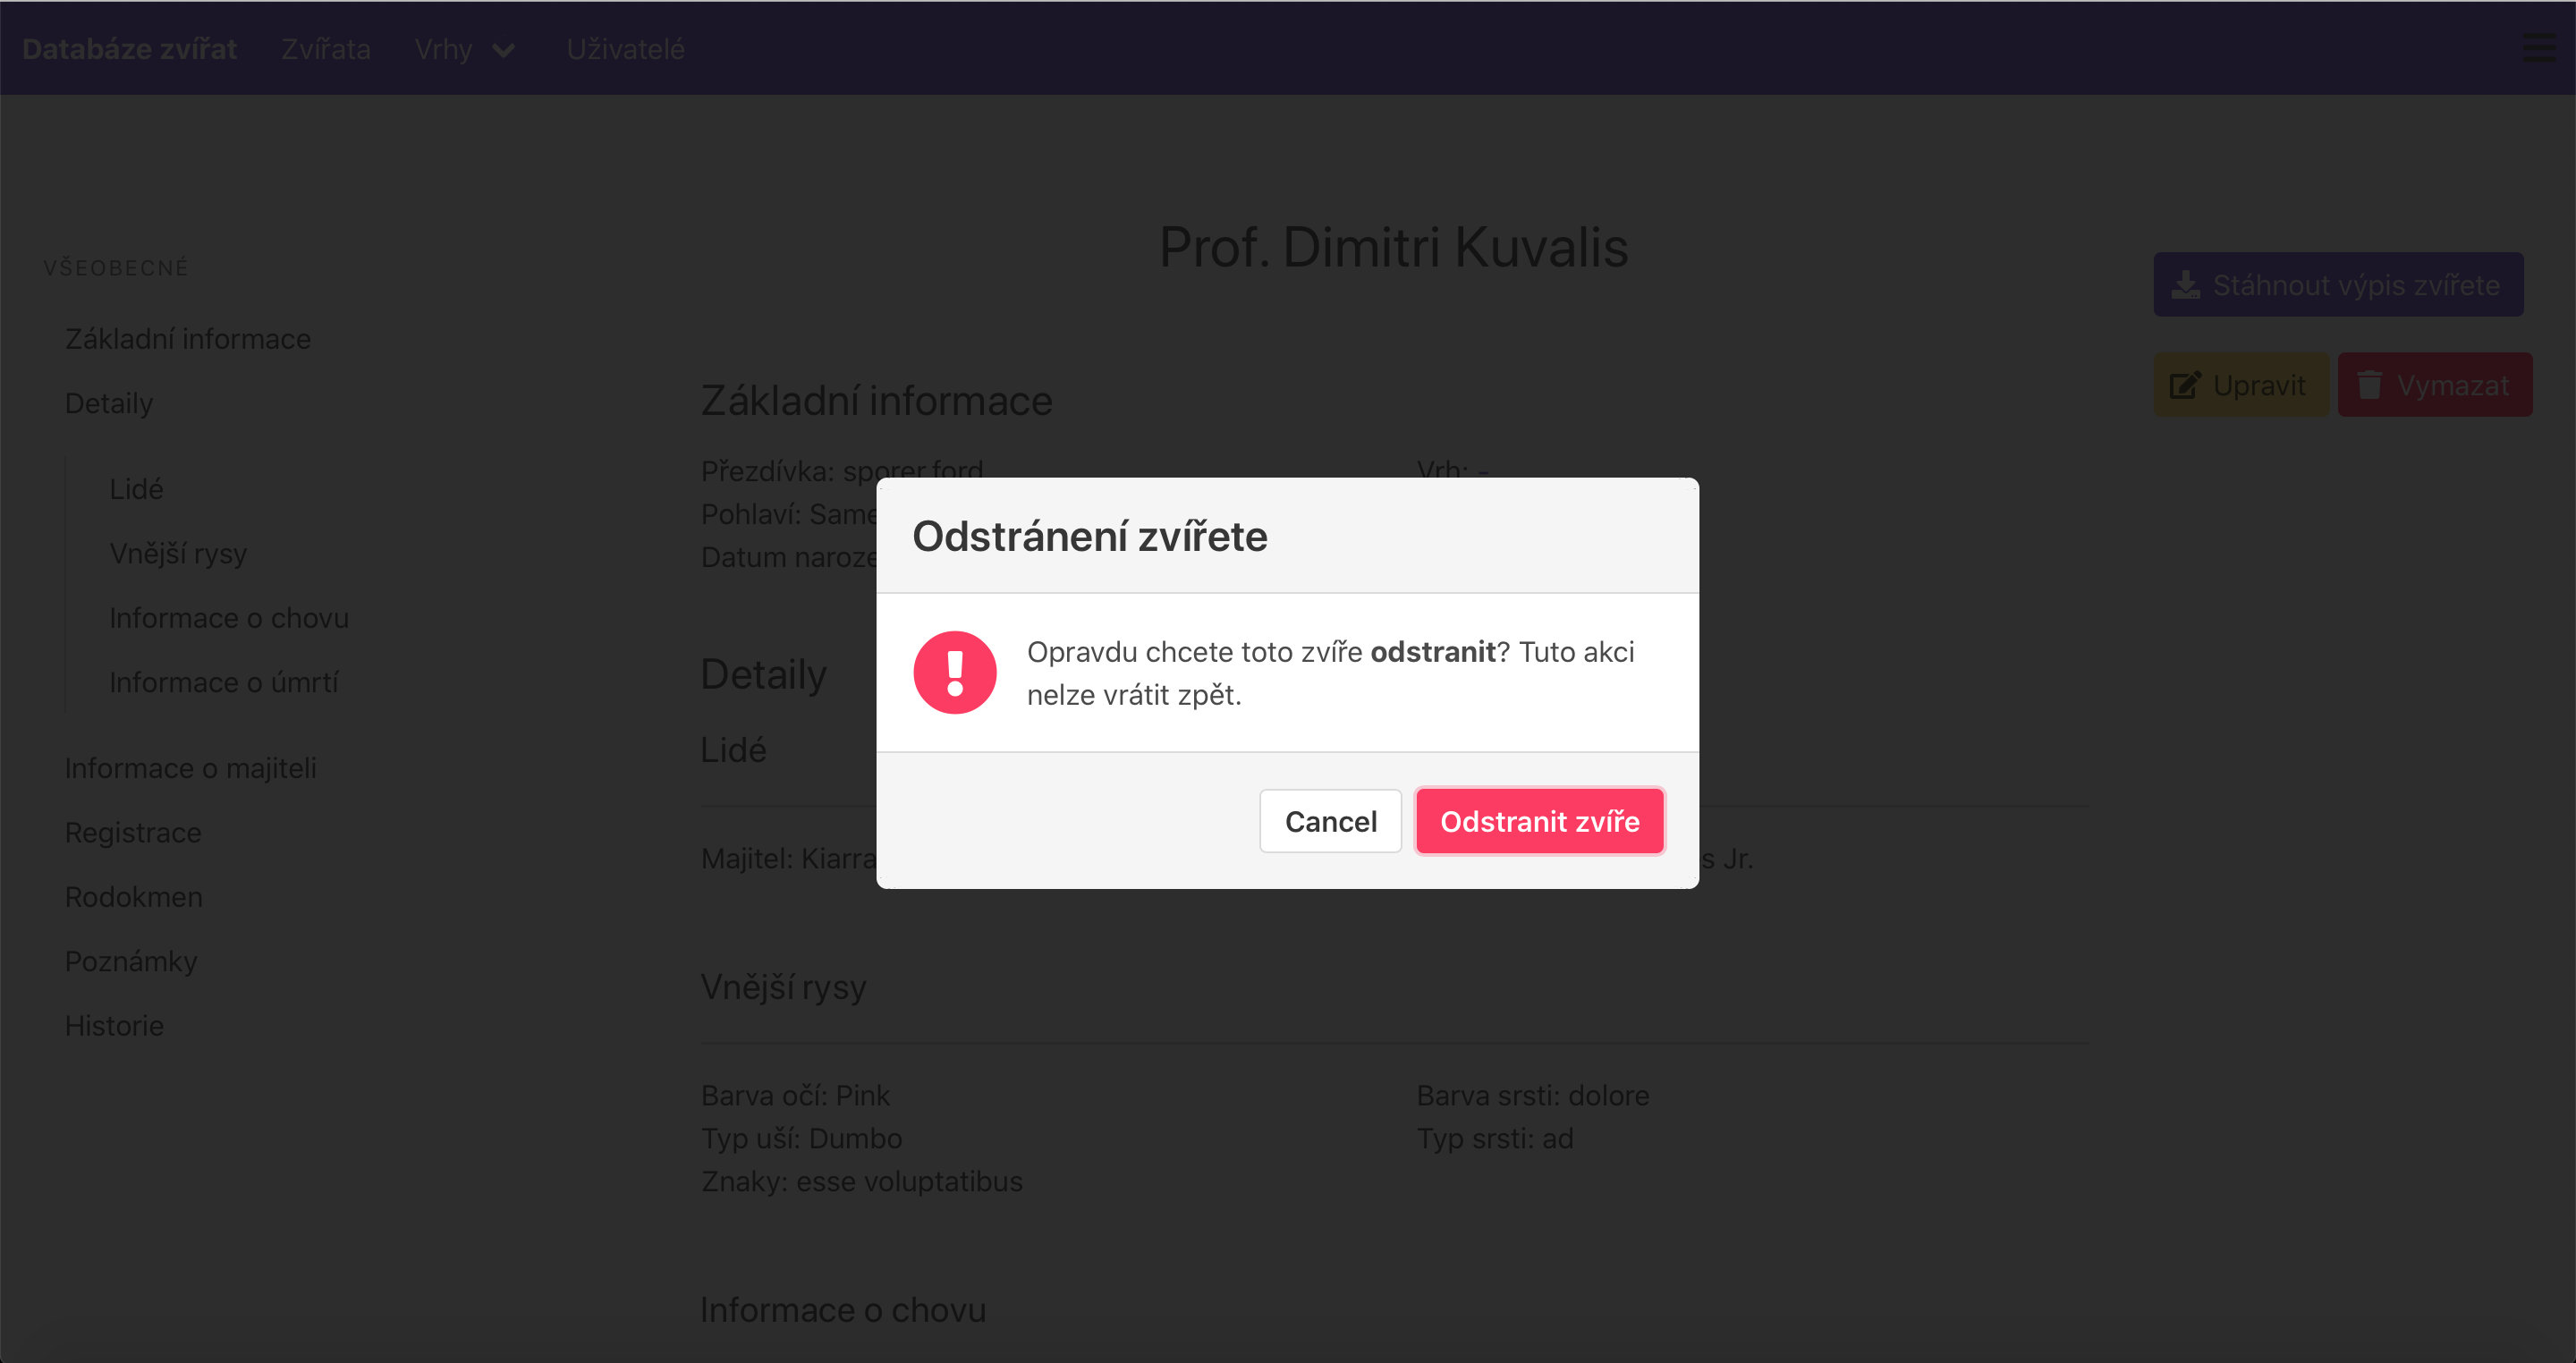
\includegraphics[width=1.0\textwidth]{media/priloha/zviera/editacia/8.png}
	\caption{Screenshot zobrazenia modálneho okna pri zvolení zmazania zvieraťa}
\end{figure}

\begin{figure}[H]
	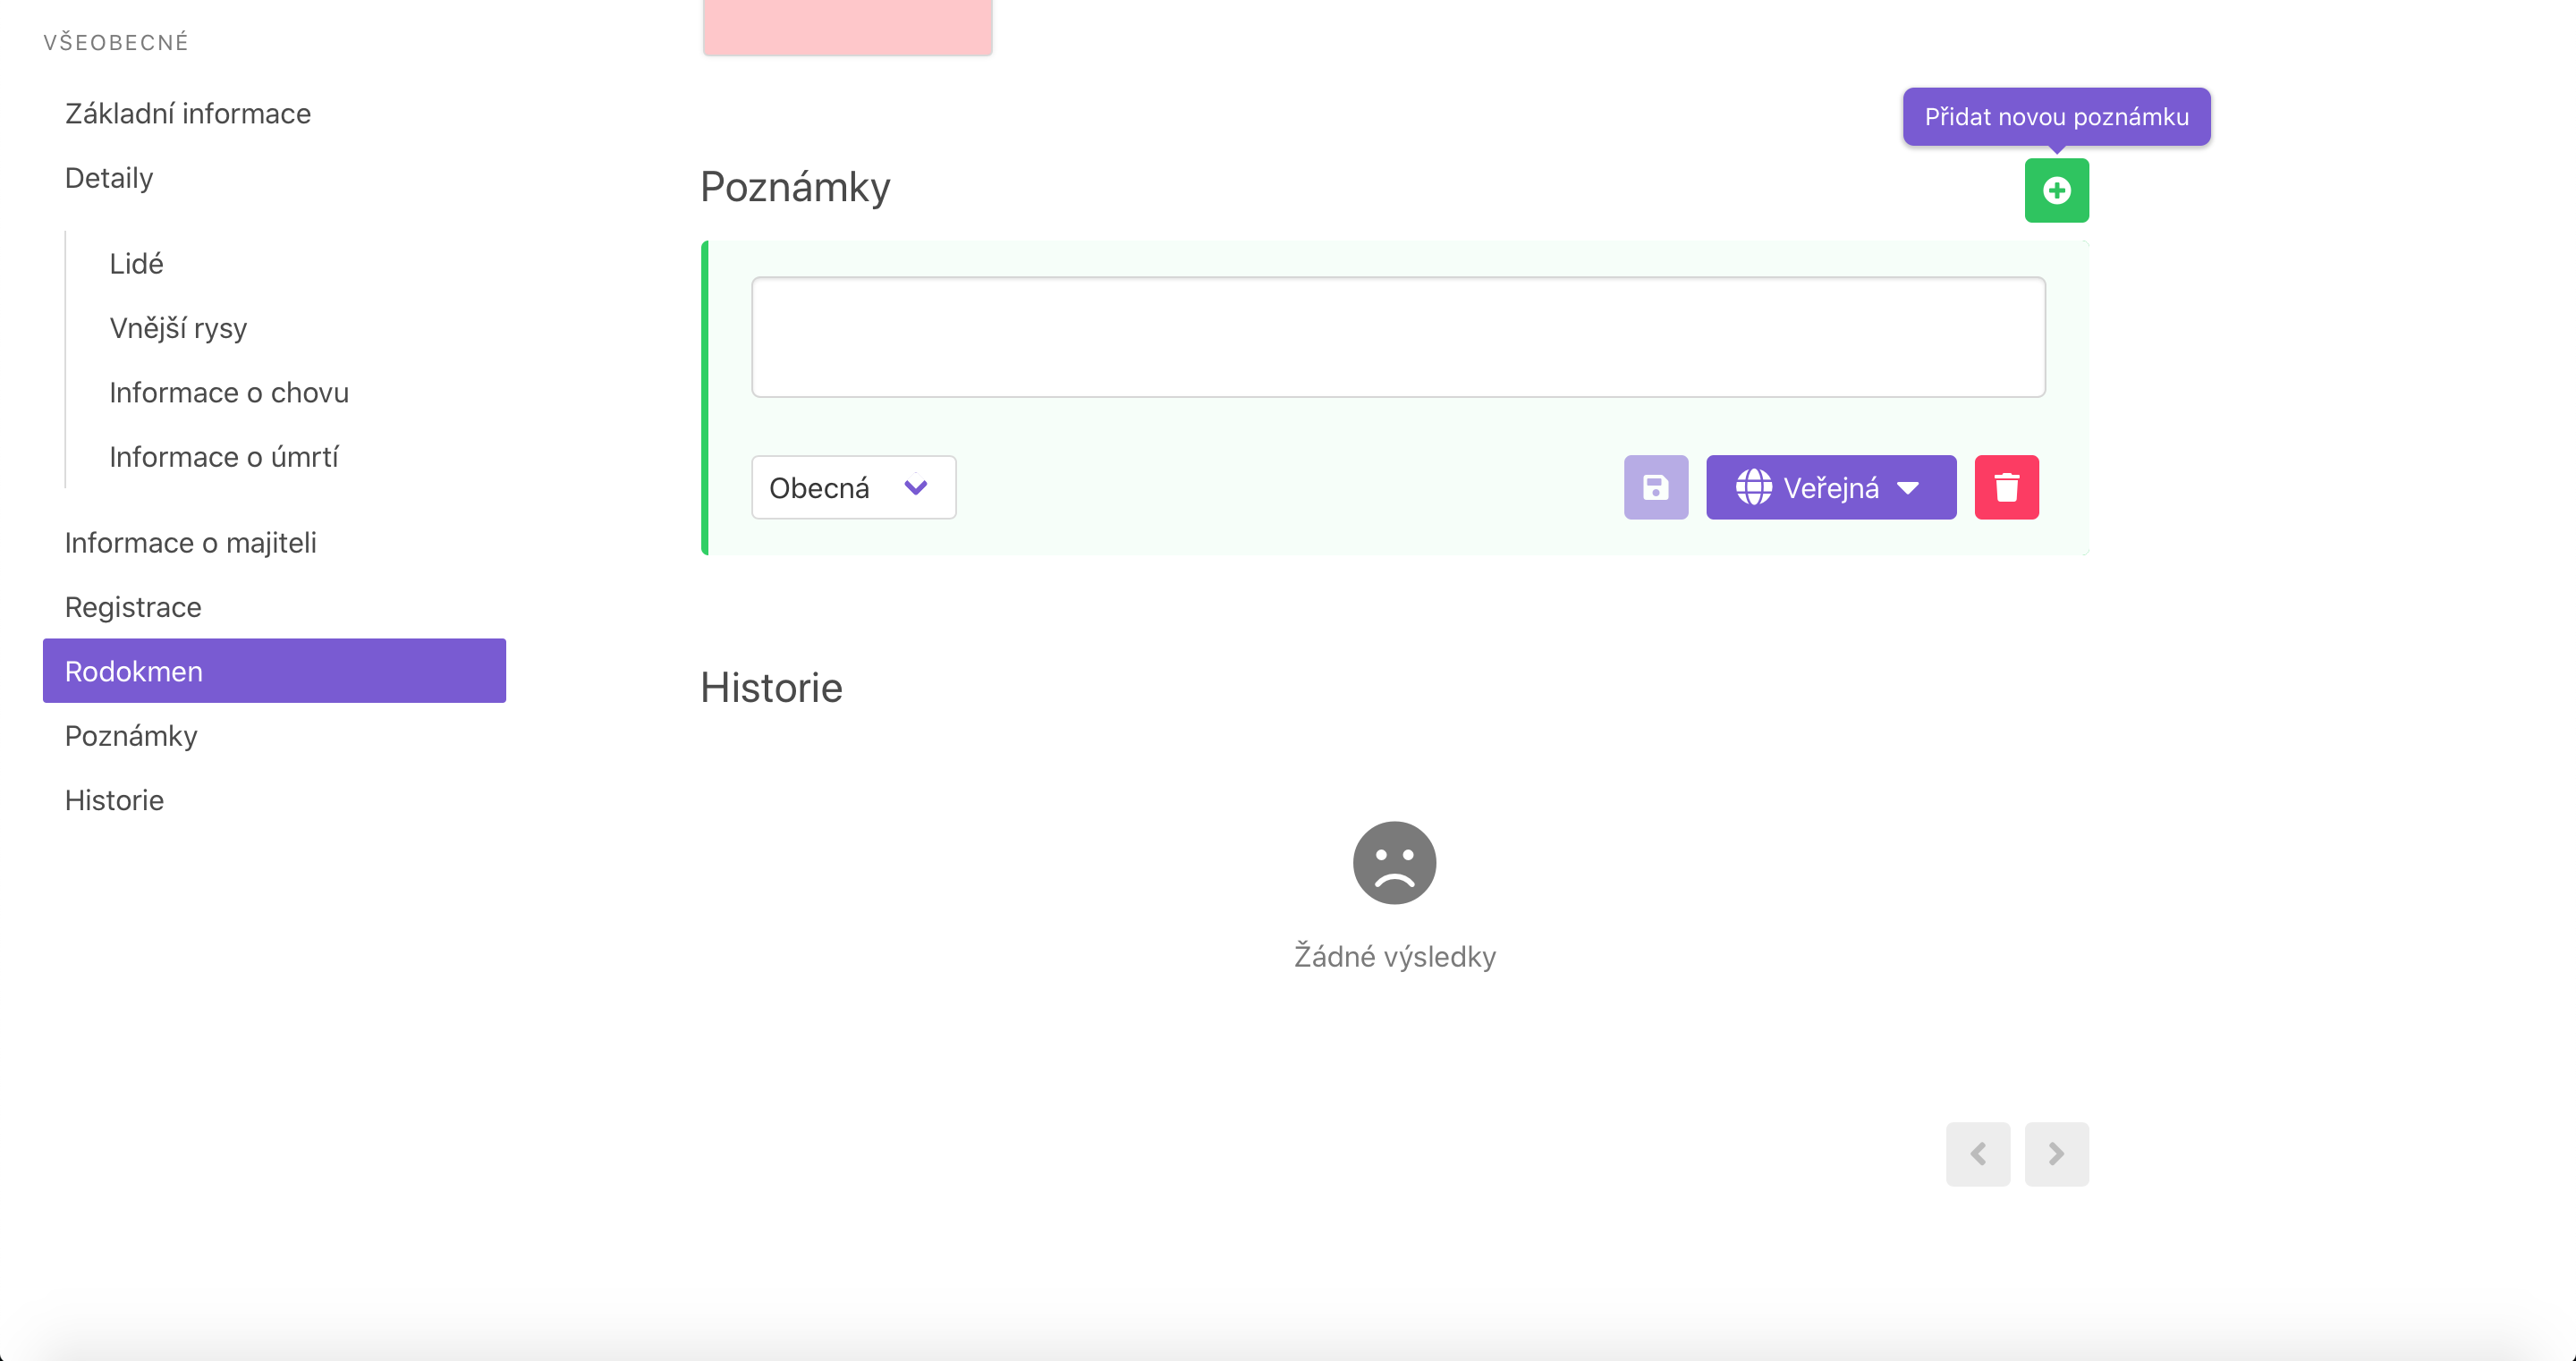
\includegraphics[width=1.0\textwidth]{media/priloha/zviera/poznamka/1.png}
	\caption{Screenshot zobrazenia poznámky po kliknutí na tlačidlo pridania novej poznámky}
\end{figure}

\vspace*{\fill}

\begin{figure}[H]
	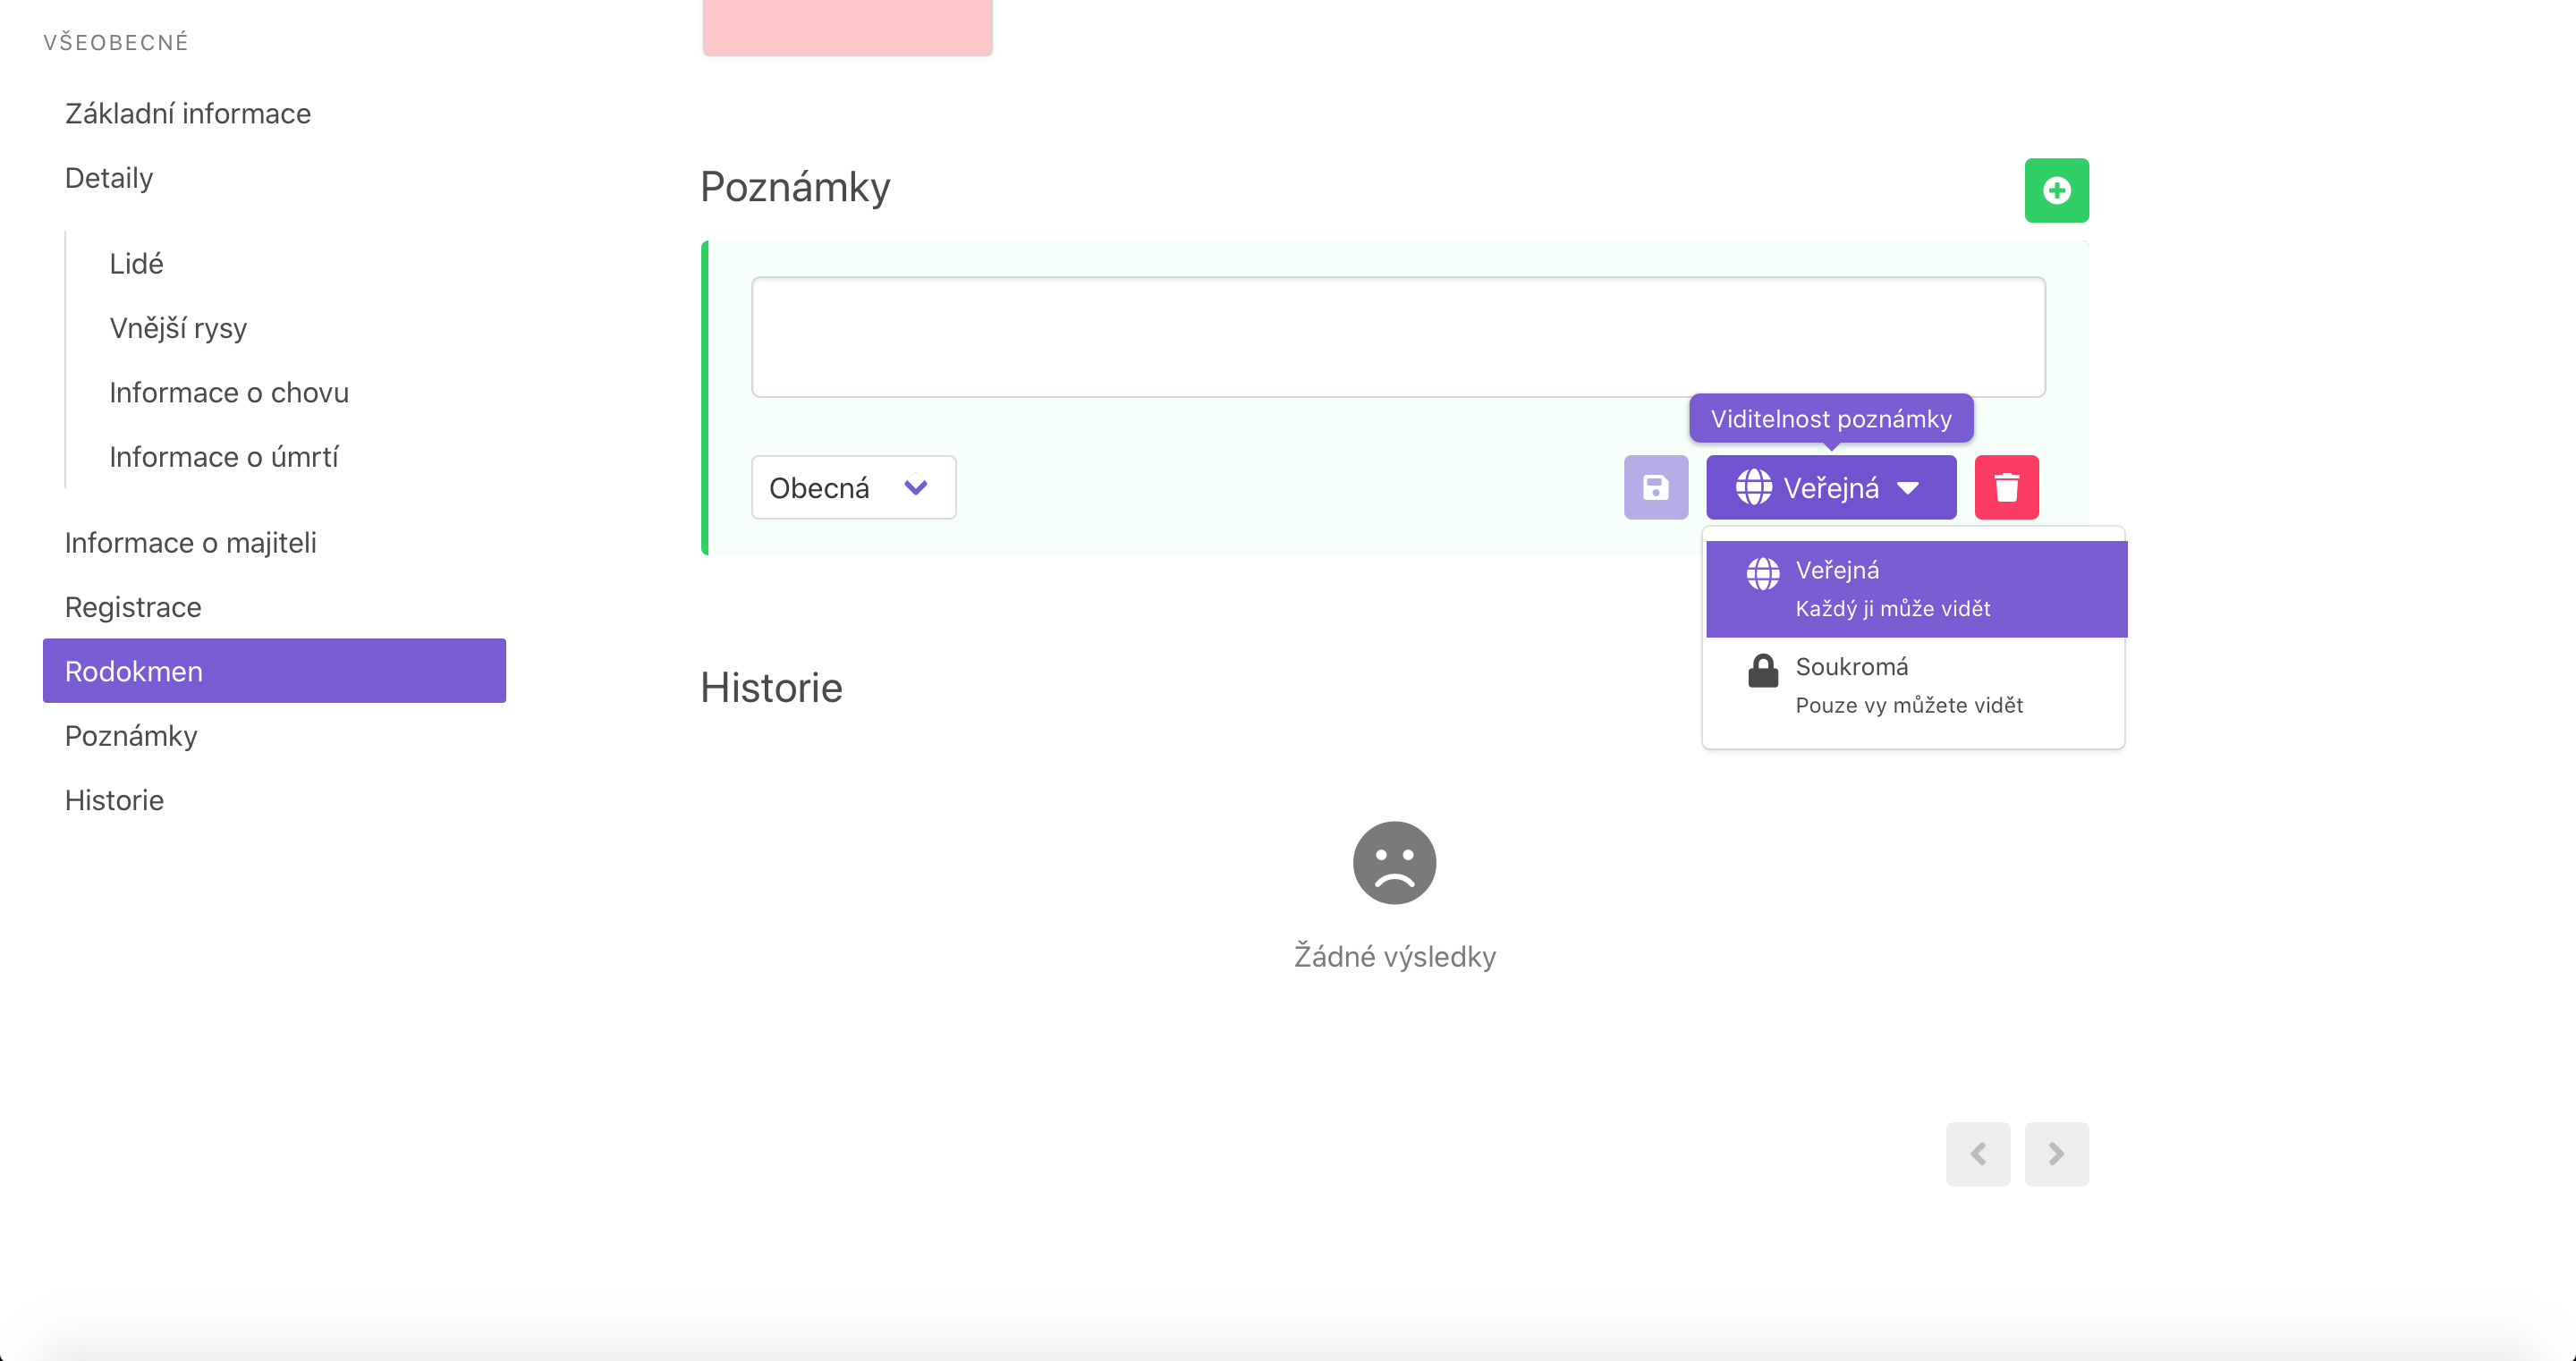
\includegraphics[width=1.0\textwidth]{media/priloha/zviera/poznamka/2.png}
	\caption{Screenshot zobrazenia viditeľnosti poznámky}
\end{figure}

\begin{figure}[H]
	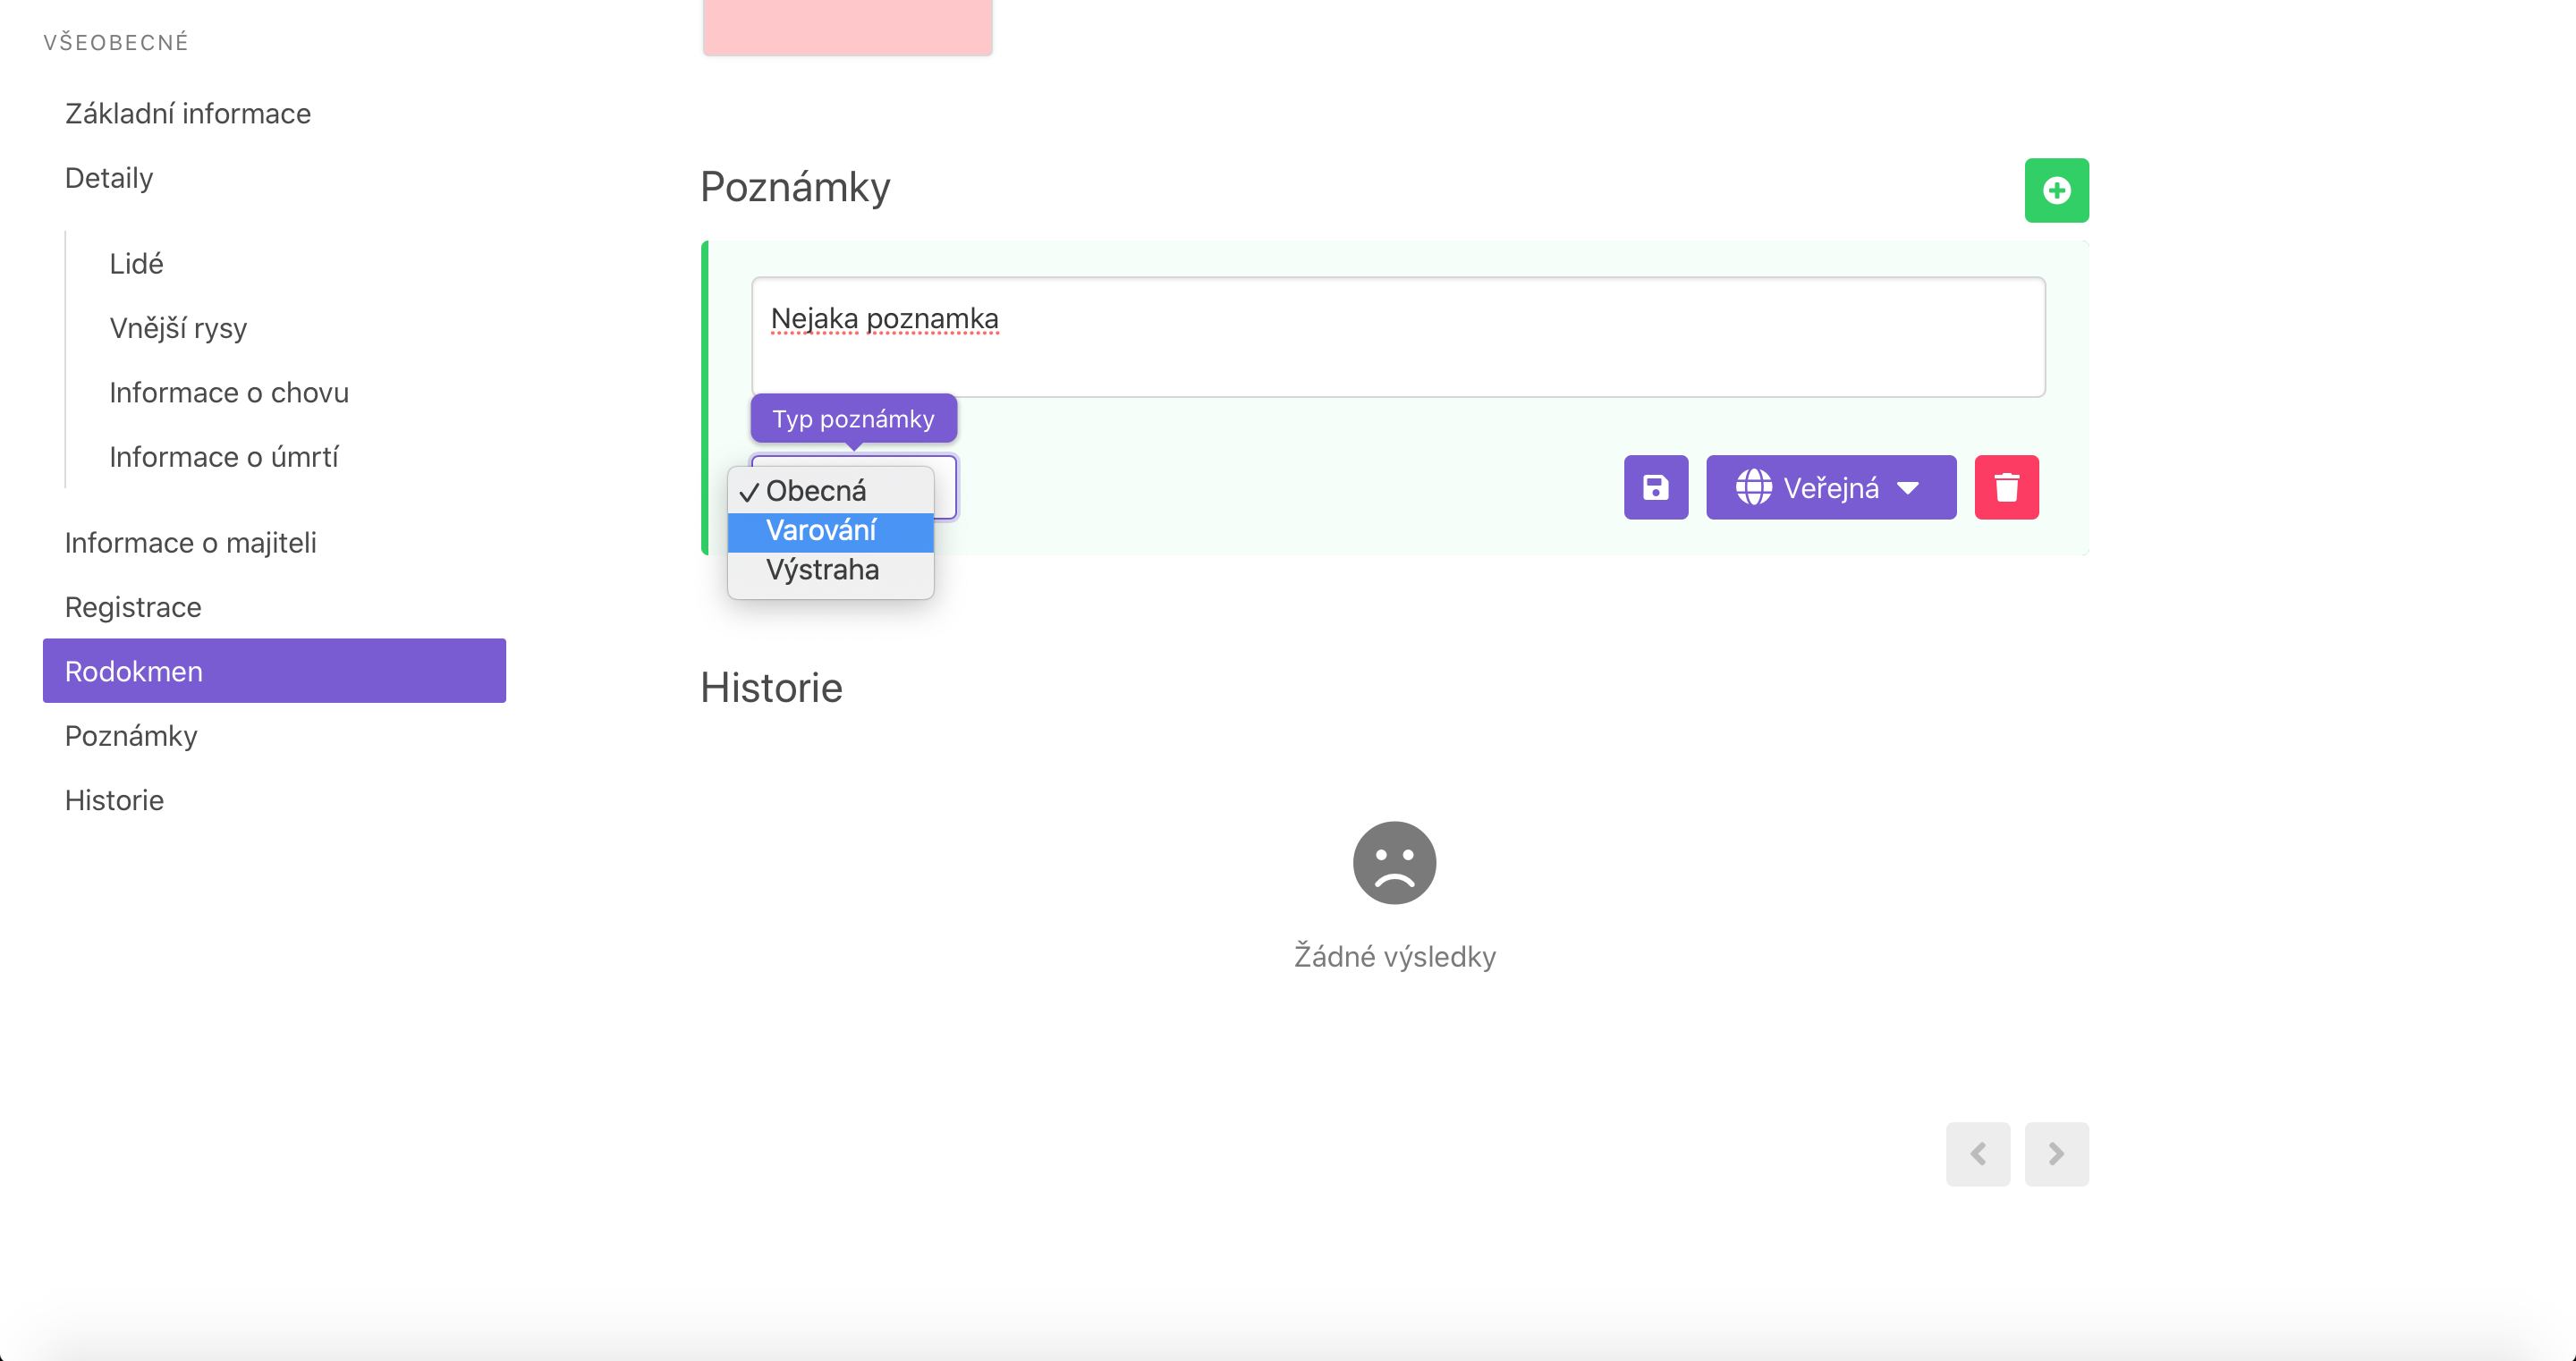
\includegraphics[width=1.0\textwidth]{media/priloha/zviera/poznamka/3.png}
	\caption{Screenshot zobrazenia typov poznámky}
\end{figure}

\vspace*{\fill}

\begin{figure}[H]
	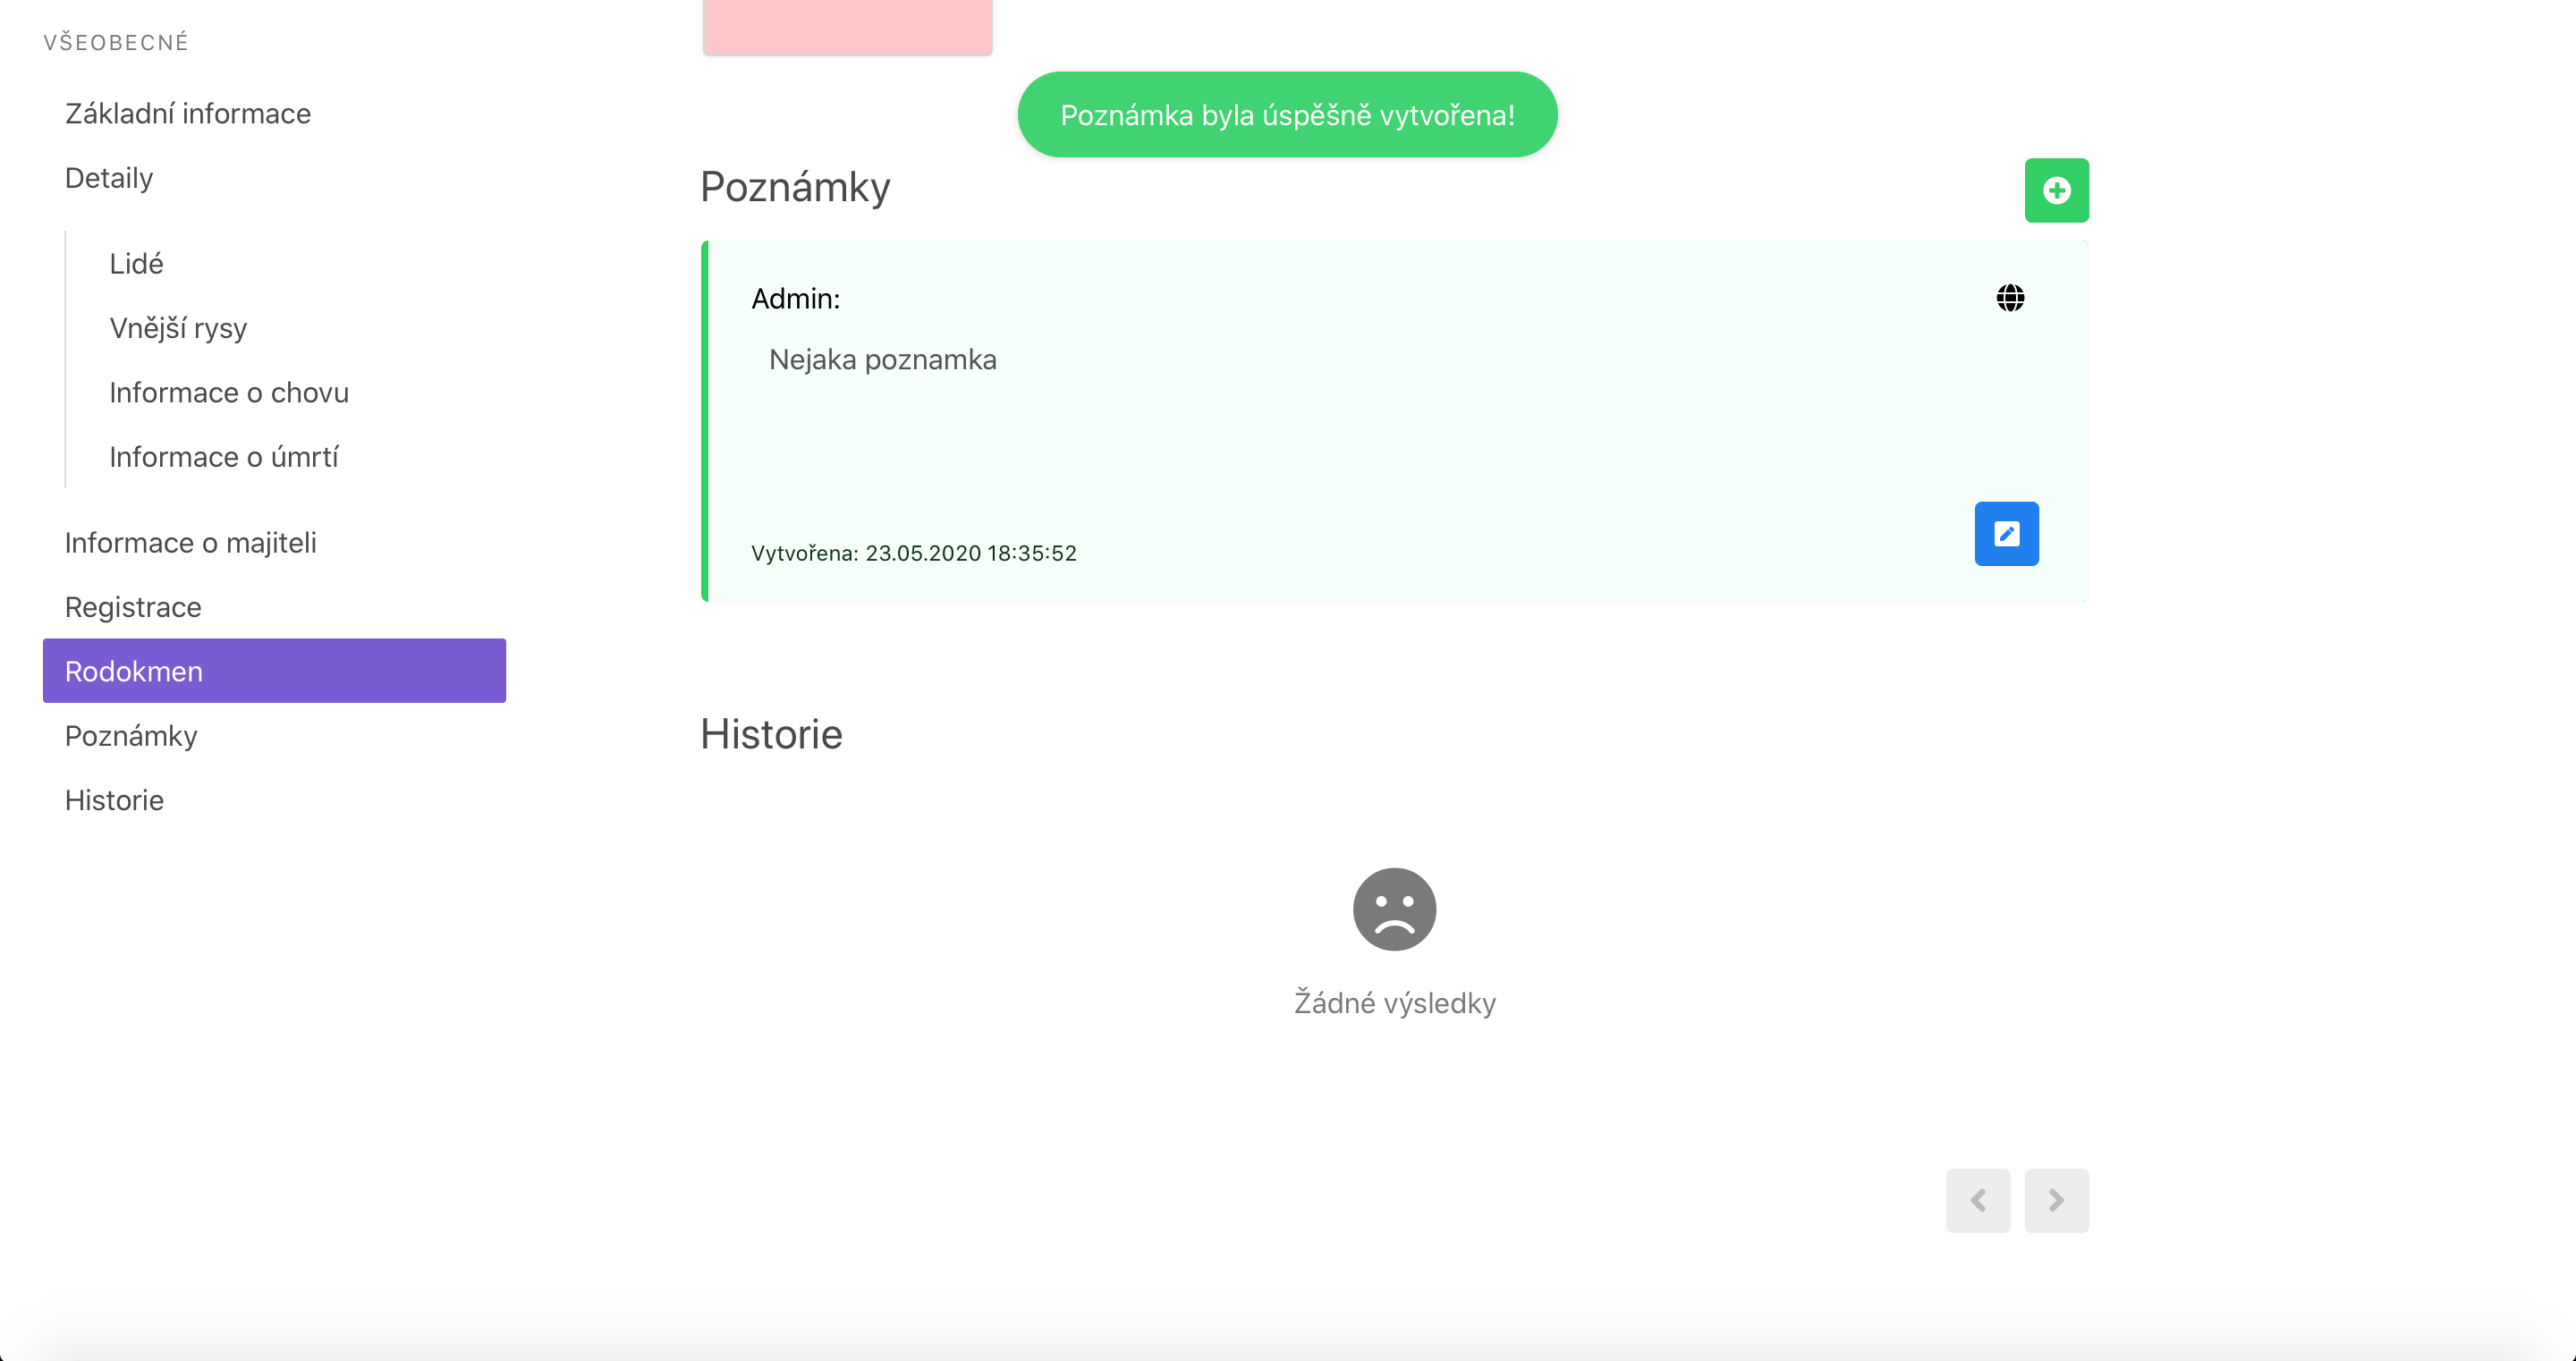
\includegraphics[width=1.0\textwidth]{media/priloha/zviera/poznamka/4.png}
	\caption{Screenshot aplikácie po vytvorení poznámky}
\end{figure}

\begin{figure}[H]
	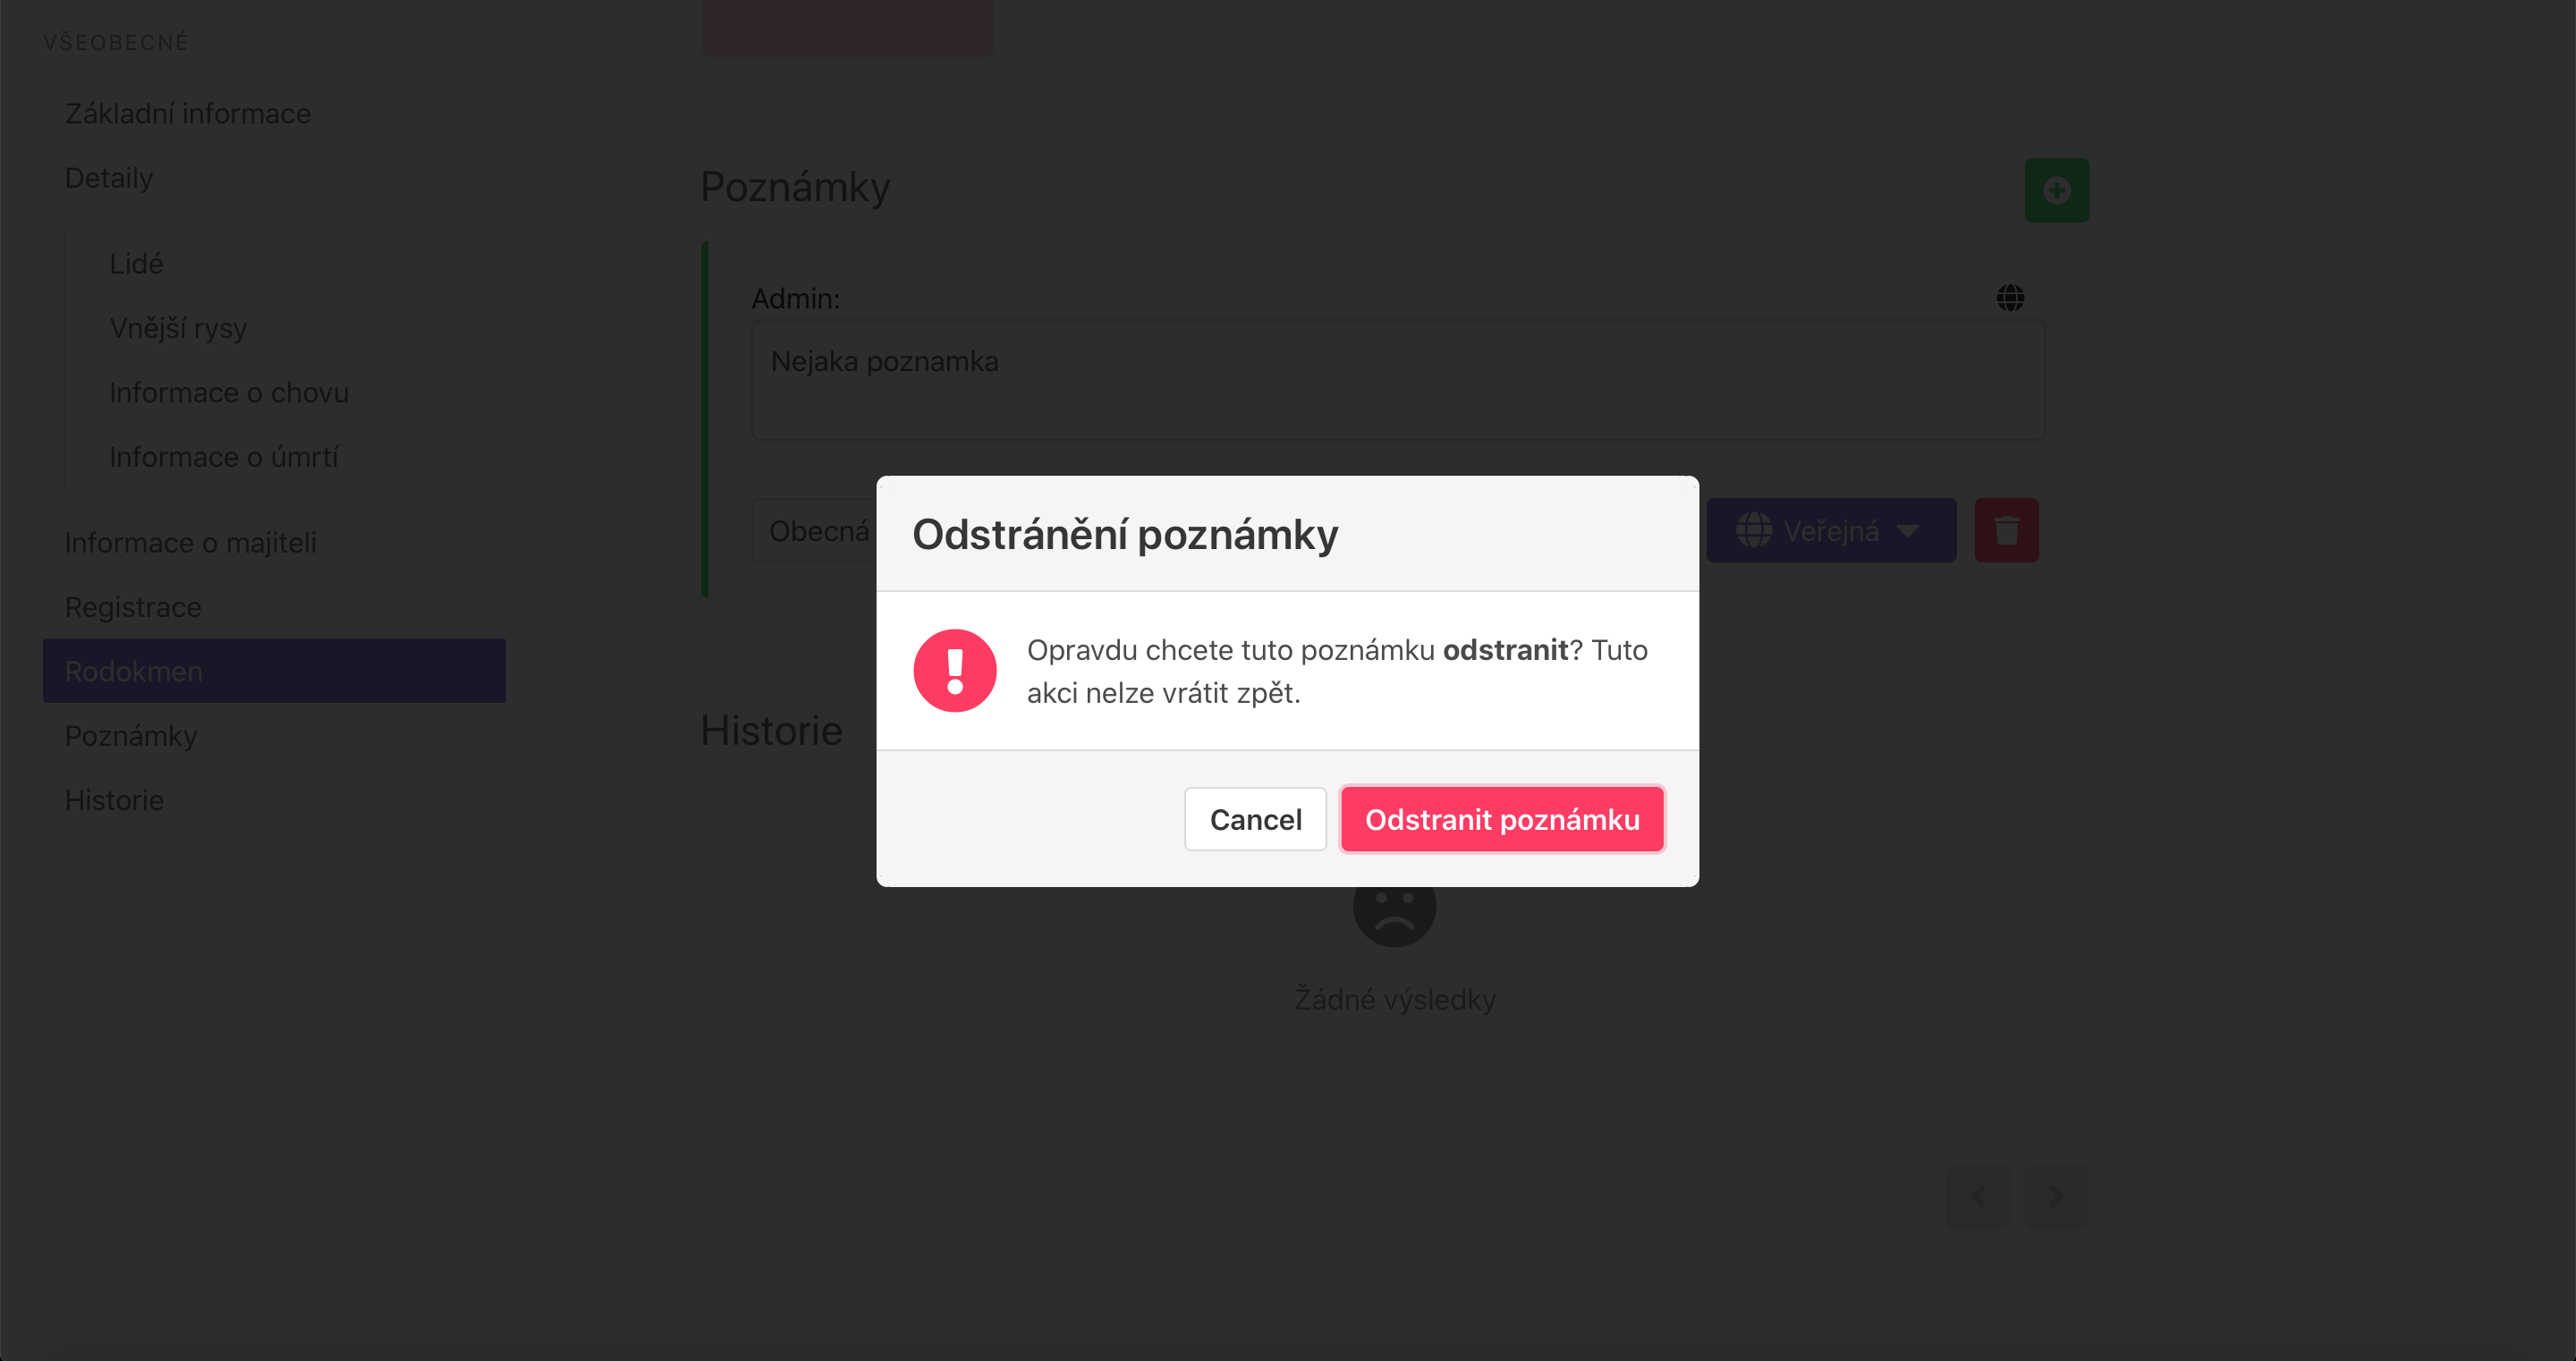
\includegraphics[width=1.0\textwidth]{media/priloha/zviera/poznamka/5.png}
	\caption{Screenshot aplikácie pri pokuse vymazať poznámku}
\end{figure}

\vspace*{\fill}

\begin{figure}[H]
	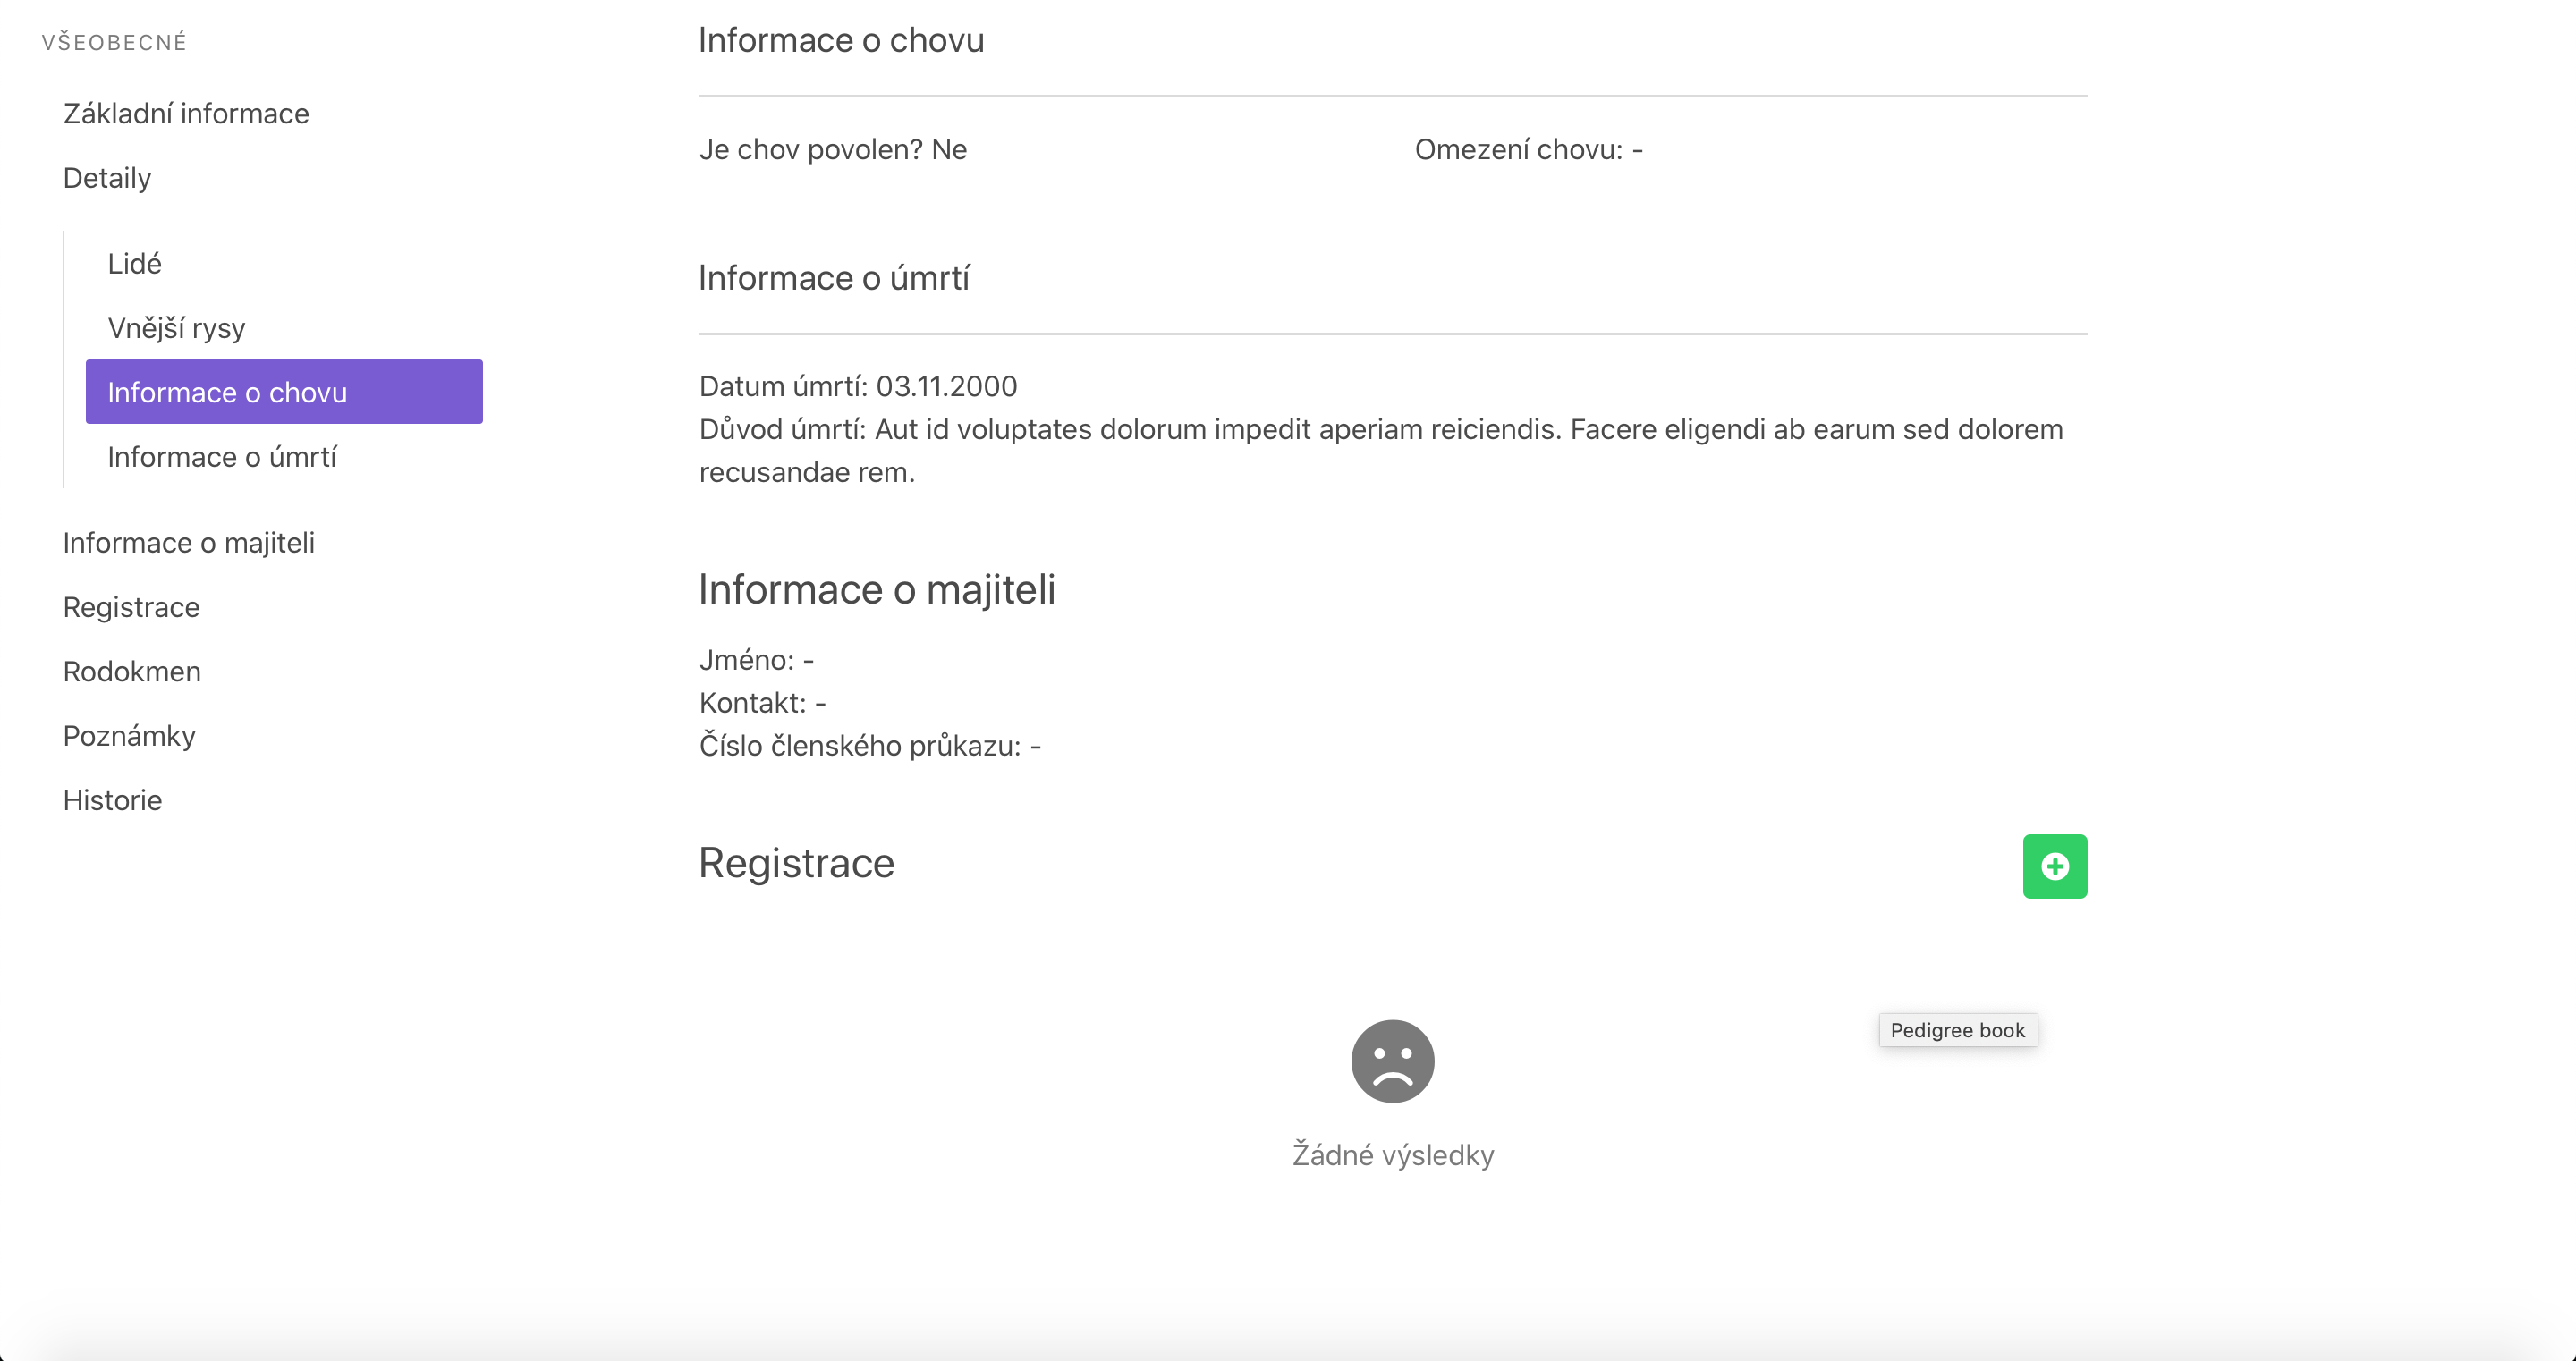
\includegraphics[width=1.0\textwidth]{media/priloha/zviera/registracia/1.png}
	\caption{Screenshot aplikácie zobrazujúci nasledujúcu sekciu zvieraťa}
\end{figure}

\begin{figure}[H]
	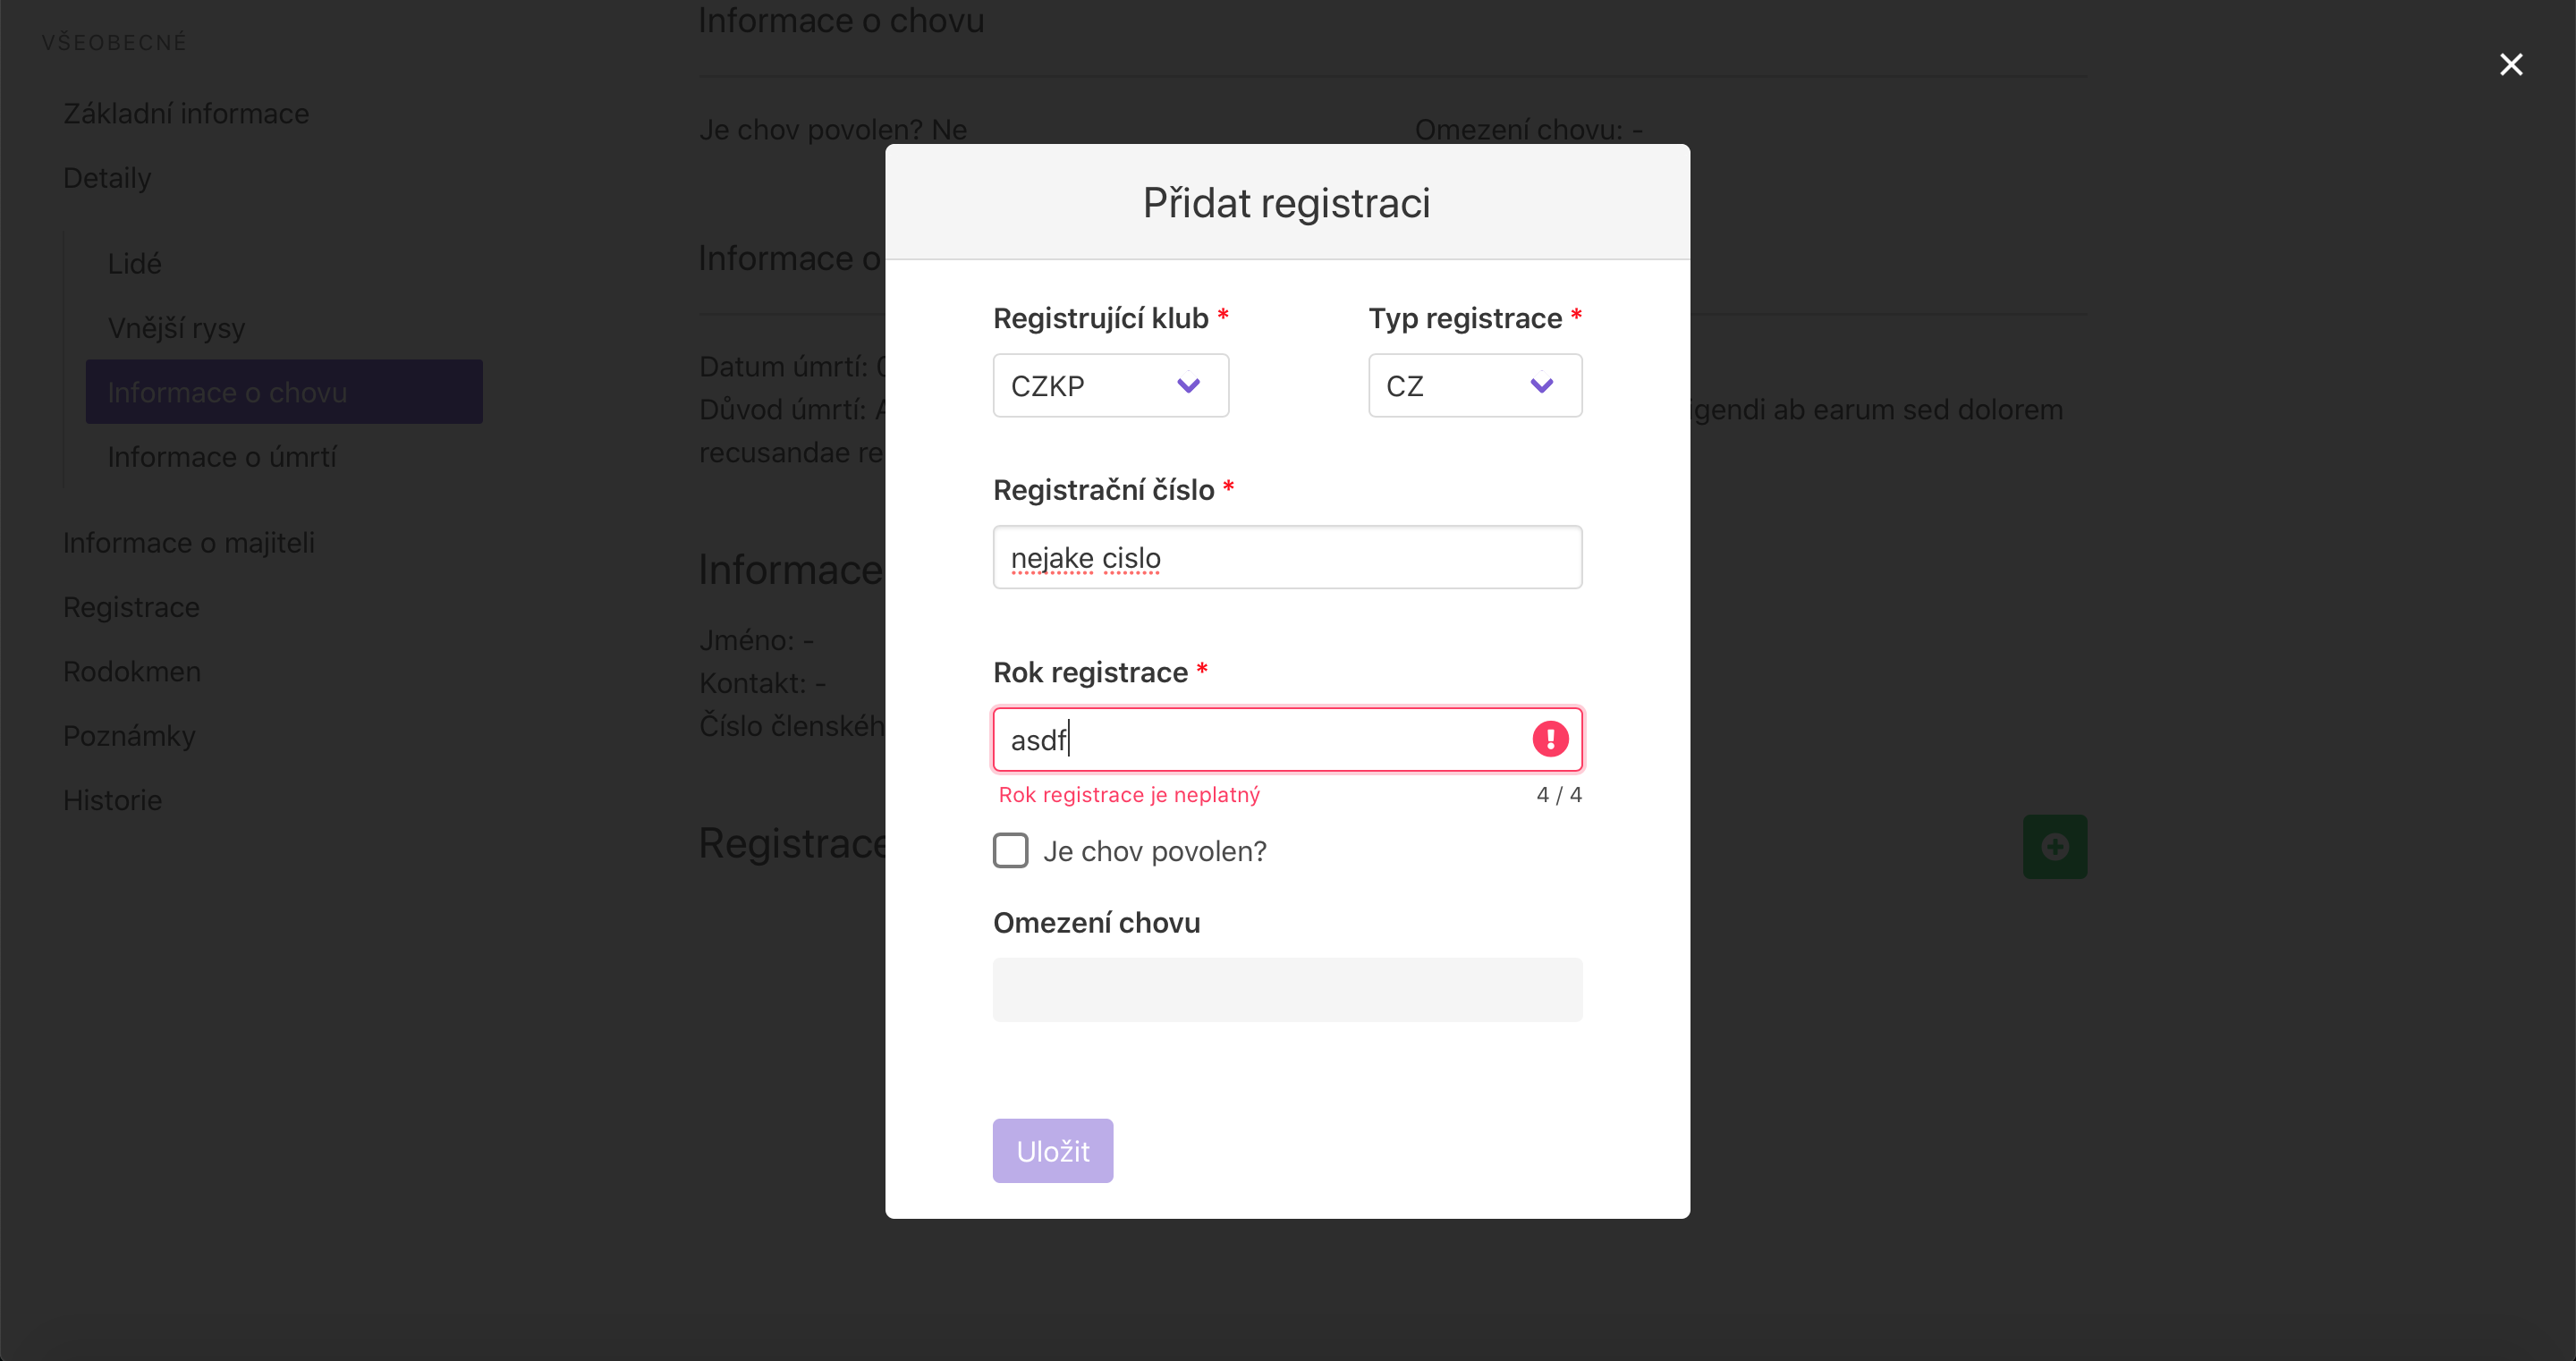
\includegraphics[width=1.0\textwidth]{media/priloha/zviera/registracia/2.png}
	\caption{Screenshot aplikácie zobrazujúci proces pridania chybnej registrácie zvieraťa}
\end{figure}

\vspace*{\fill}

\begin{figure}[H]
	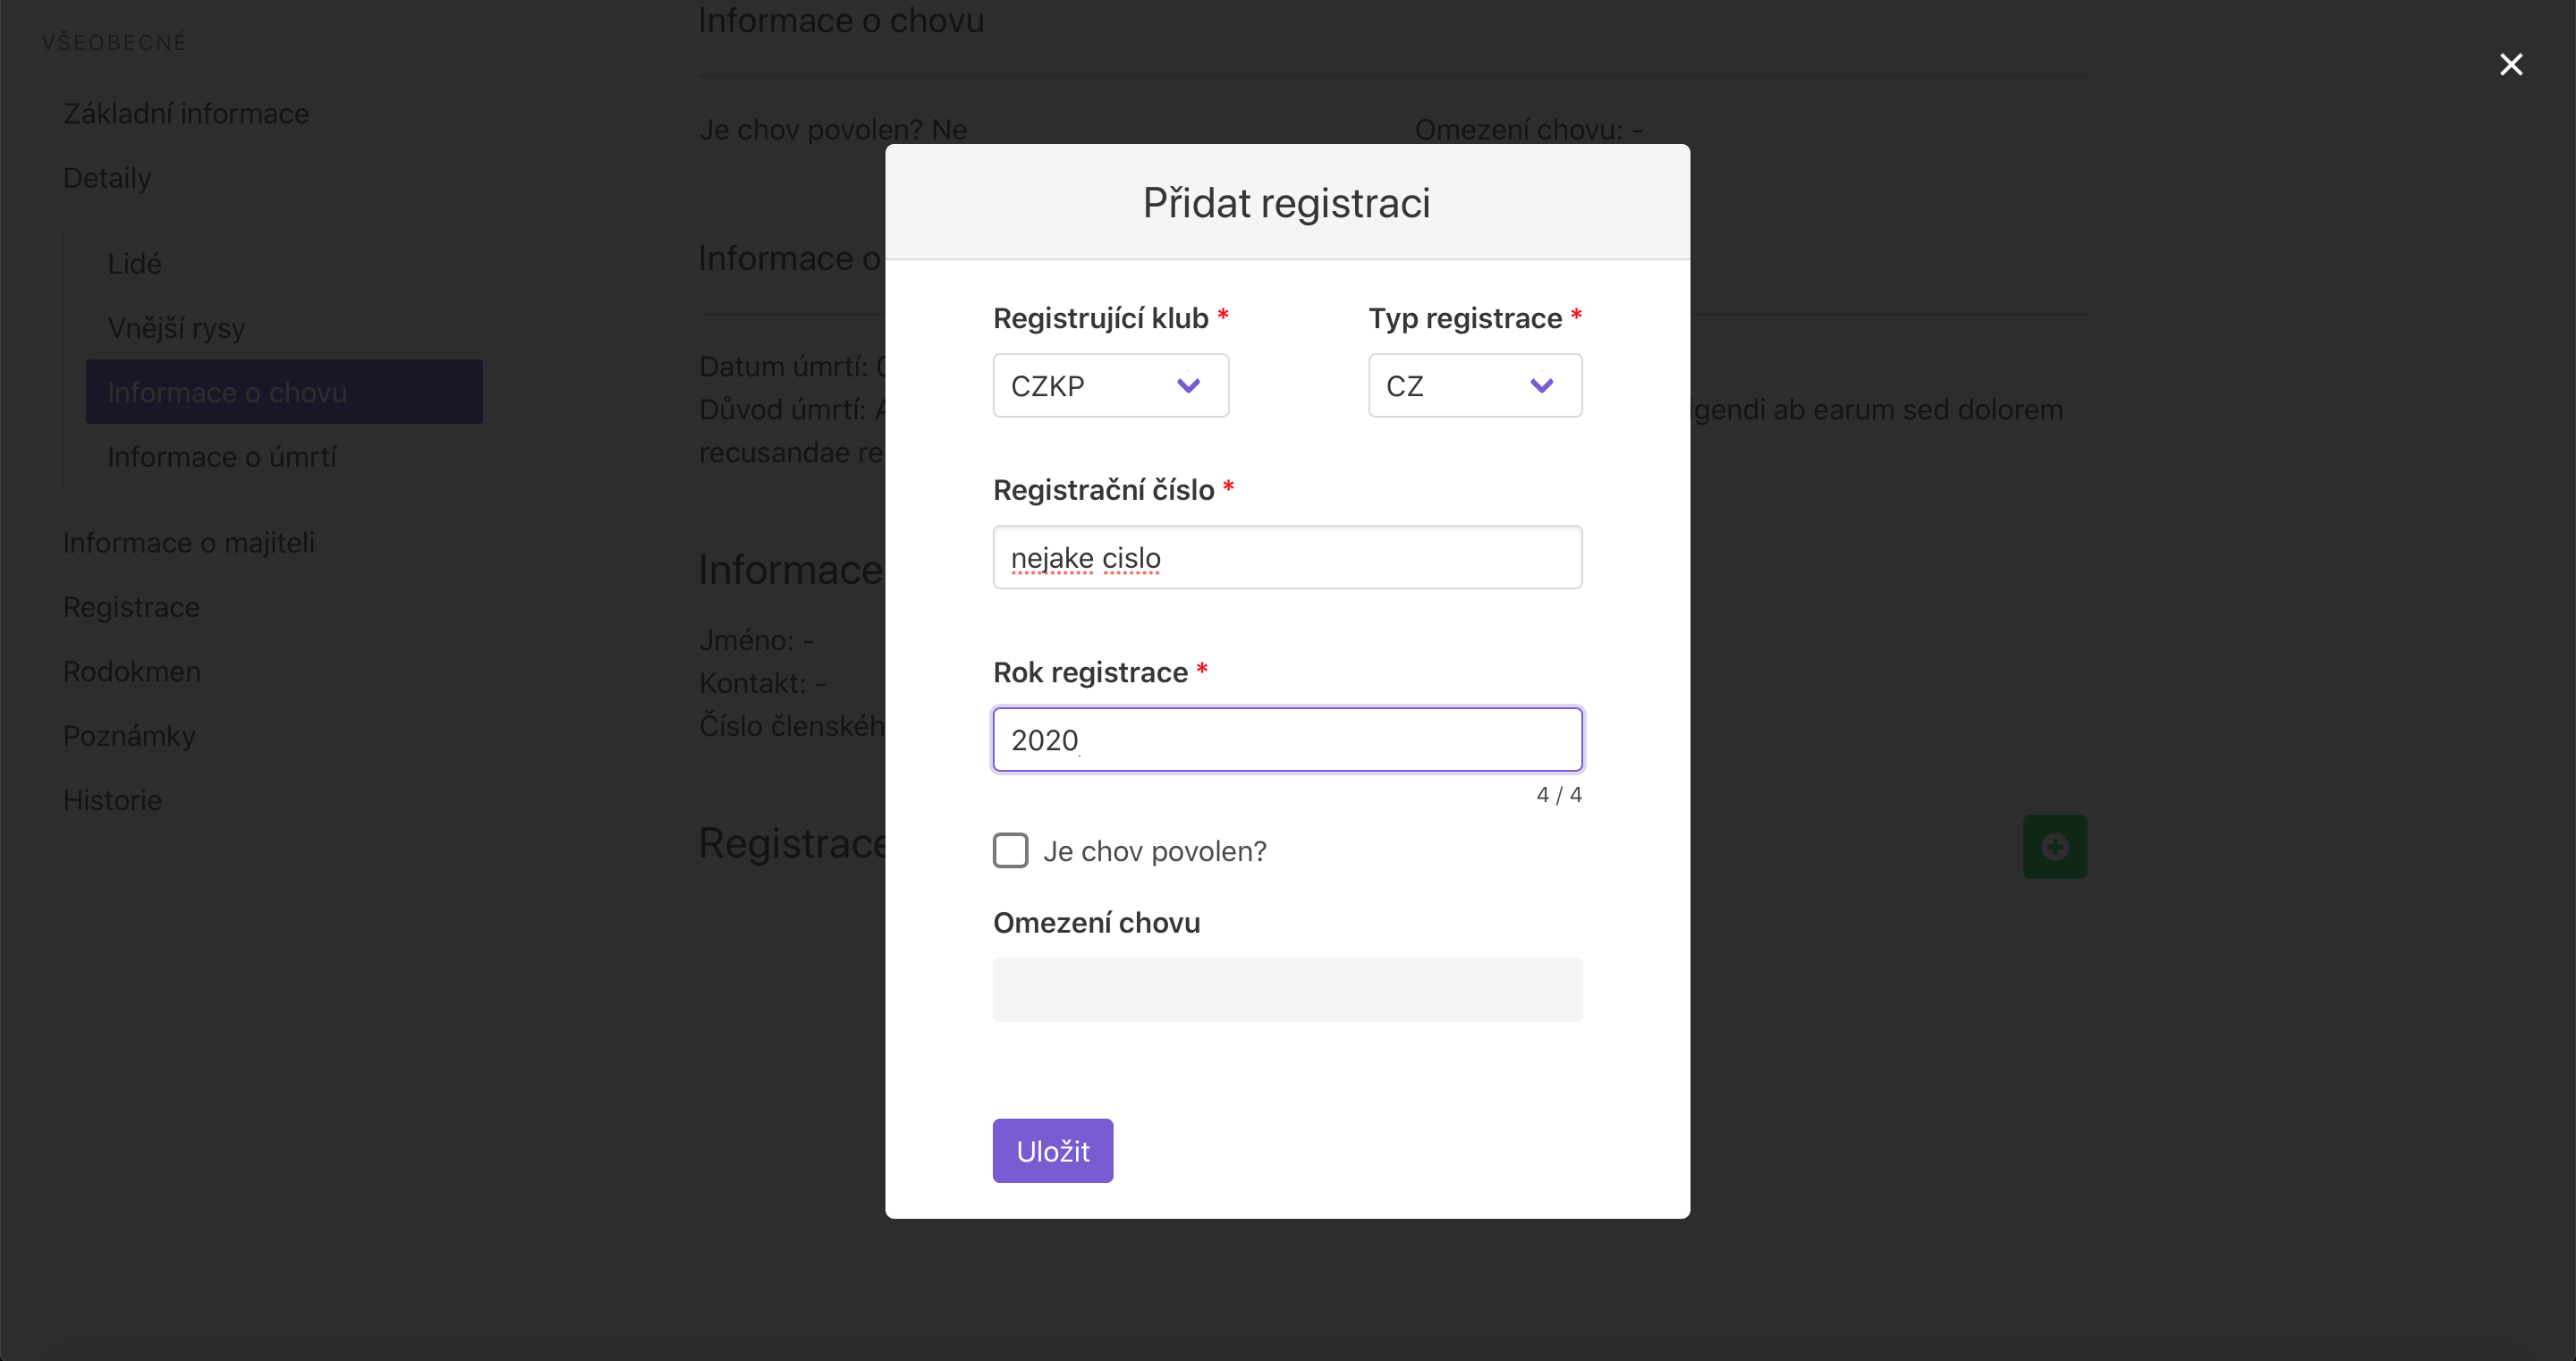
\includegraphics[width=1.0\textwidth]{media/priloha/zviera/registracia/3.png}
	\caption{Screenshot aplikácie zobrazujúci proces pridania správnej regsitrácie zvieraťa}
\end{figure}

\begin{figure}[H]
	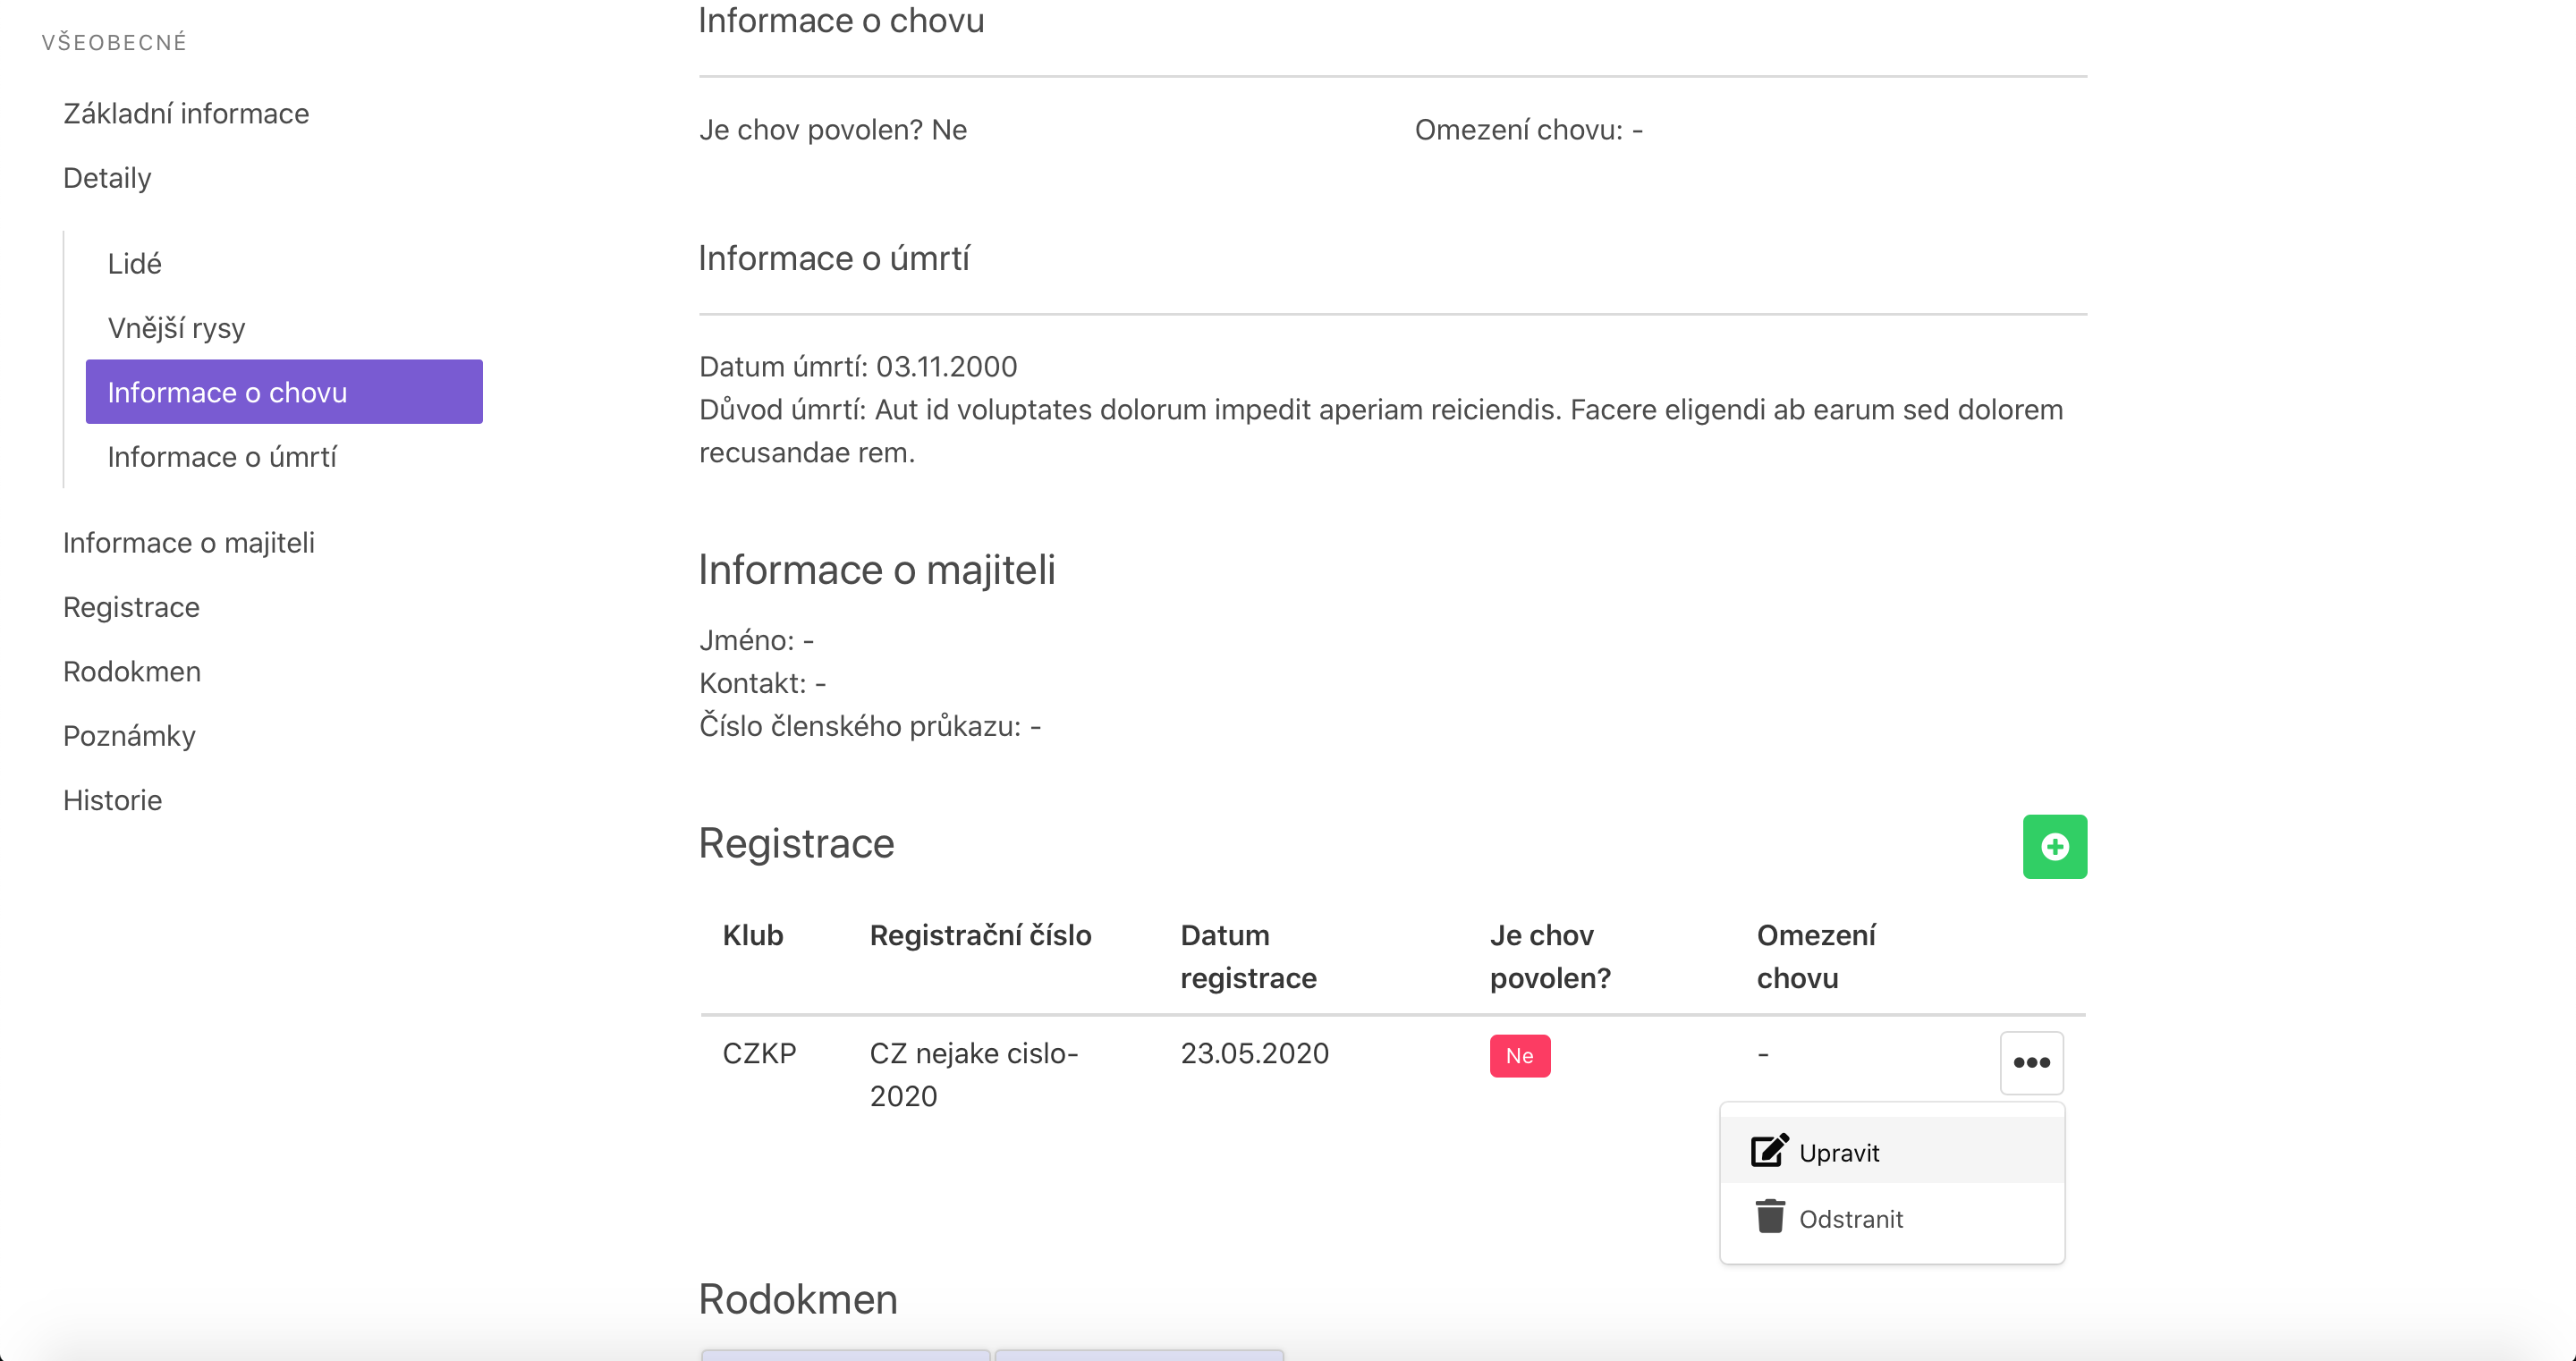
\includegraphics[width=1.0\textwidth]{media/priloha/zviera/registracia/4.png}
	\caption{Screenshot aplikácie zobrazujúci registráciu zvieraťa po jej pridaní}
\end{figure}

\vspace*{\fill}

\begin{figure}[H]
	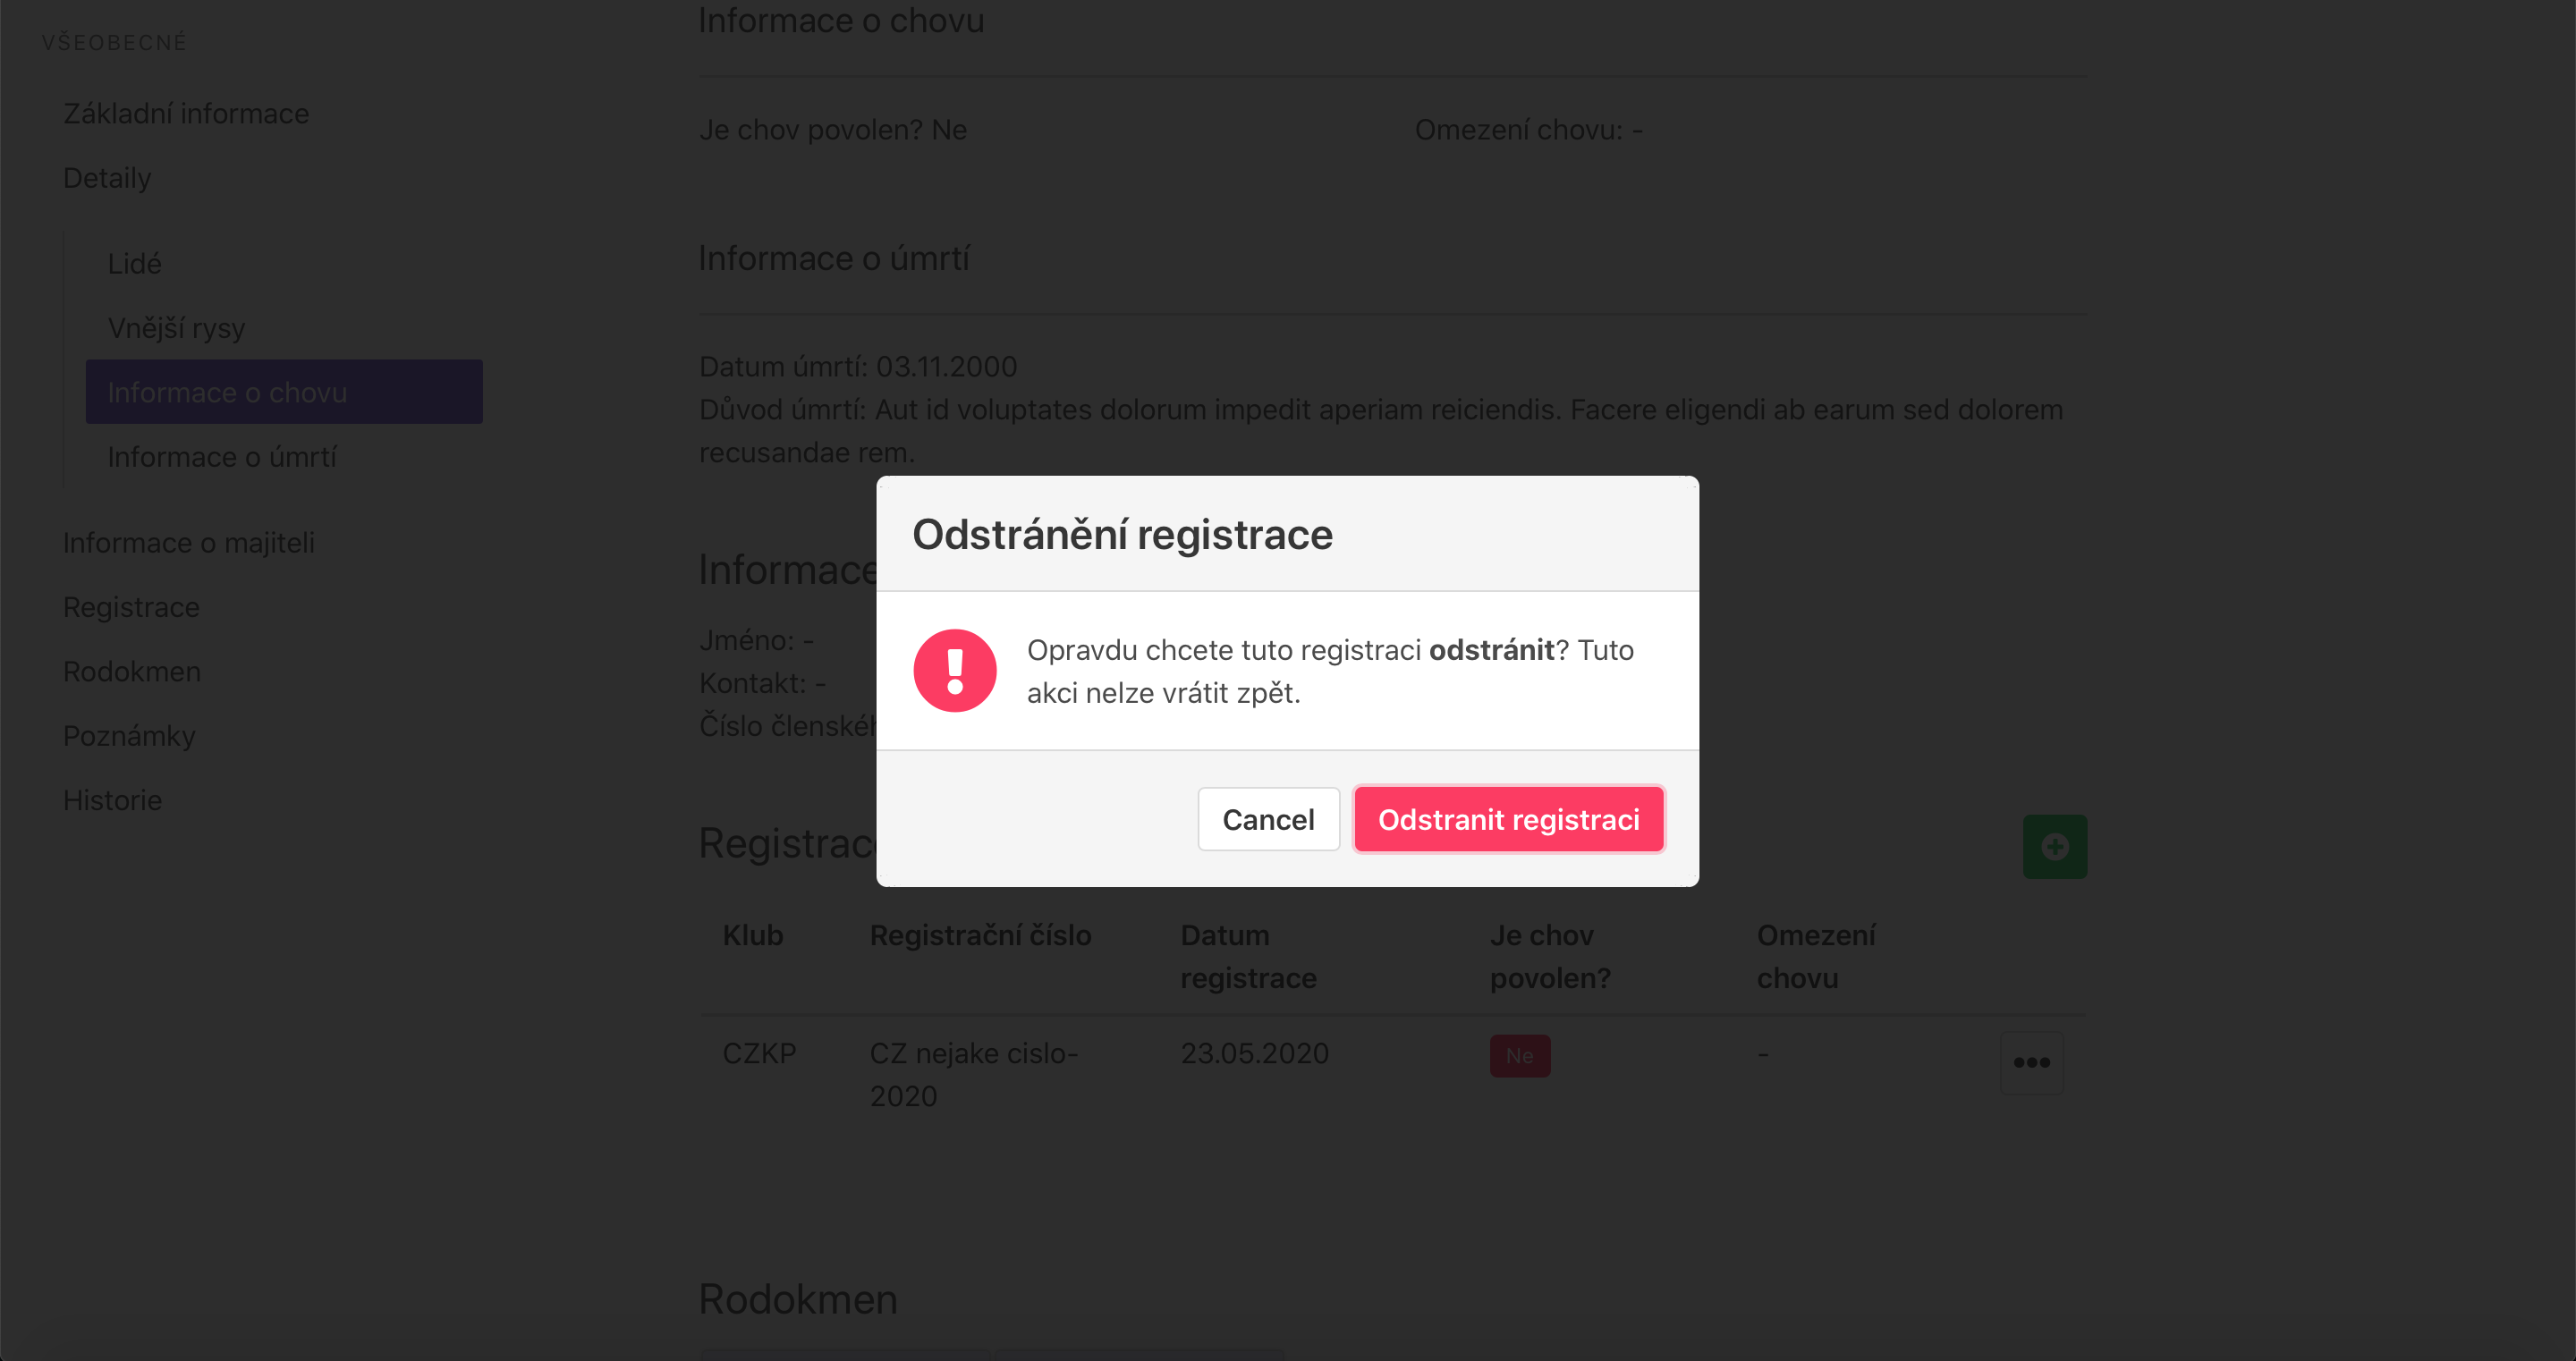
\includegraphics[width=1.0\textwidth]{media/priloha/zviera/registracia/5.png}
	\caption{Screenshot modálneho okna aplikácie pri ostránení registrácie}
\end{figure}

\begin{figure}[H]
	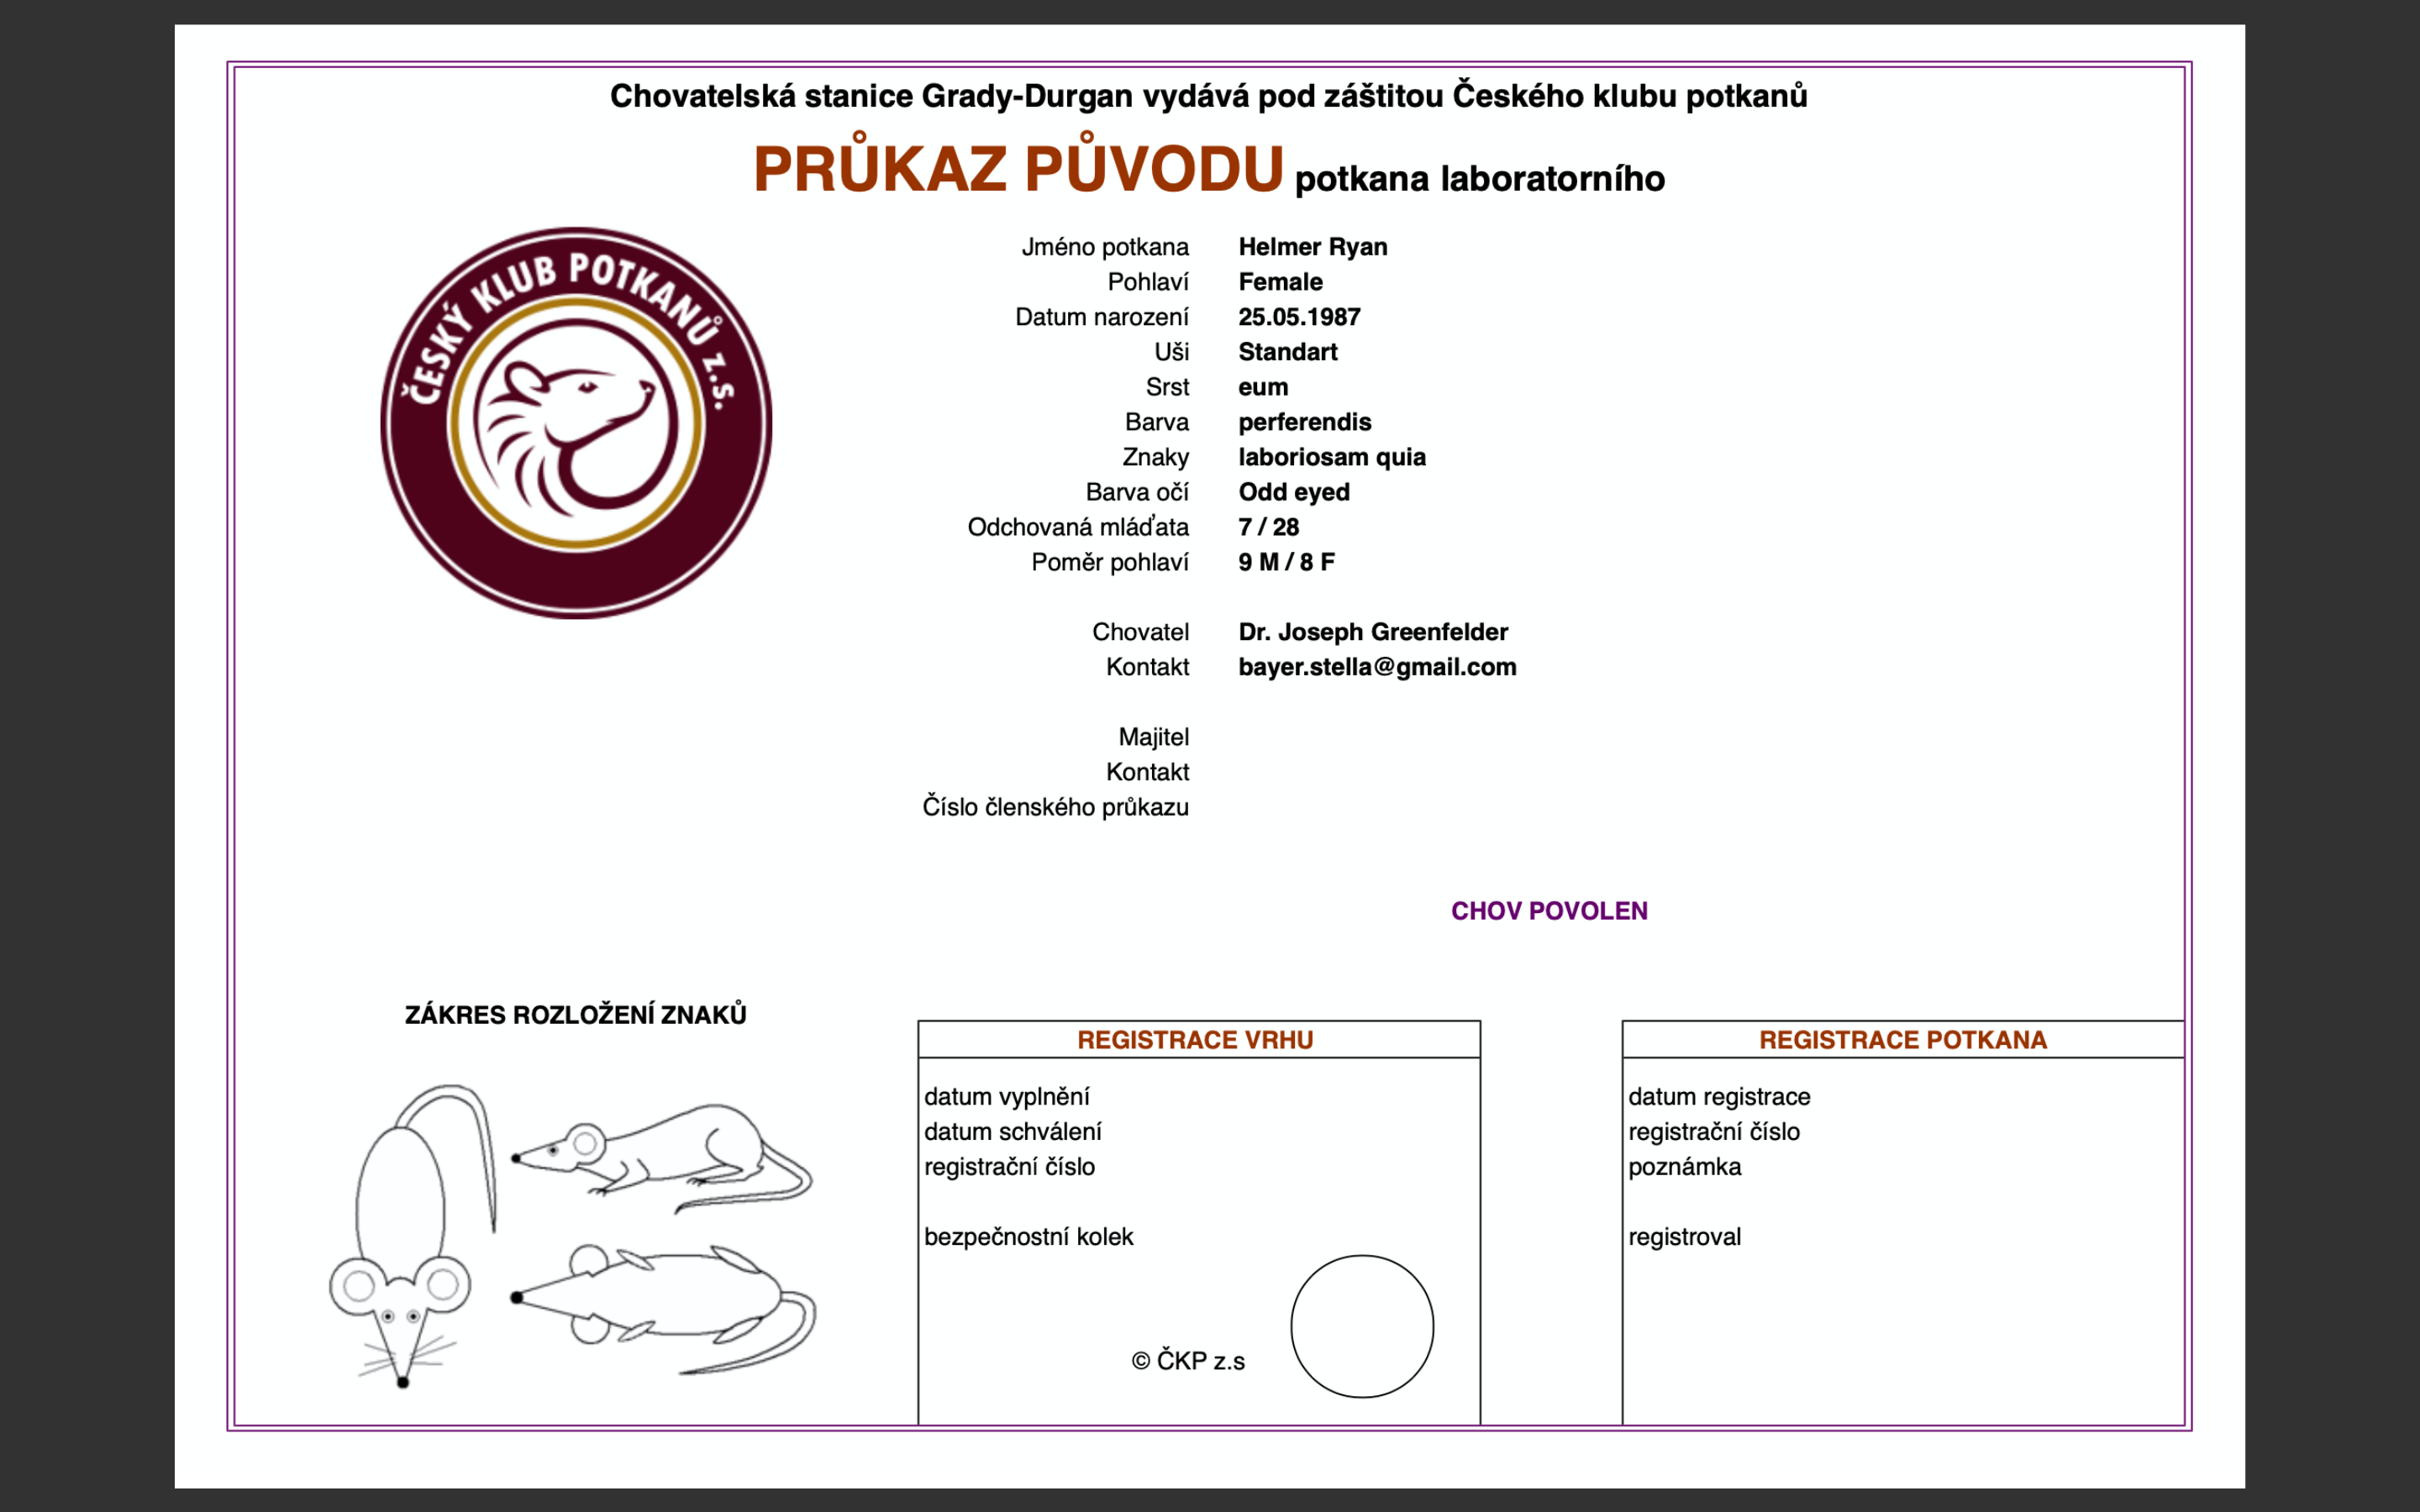
\includegraphics[width=1.0\textwidth]{media/priloha/vseobecne/pdf/1.png}
	\caption{Screenshot zobrazujúci prvú stranu vygenerovaného PDF súbor zvieraťa}
\end{figure}

\vspace*{\fill}

\begin{figure}[H]
	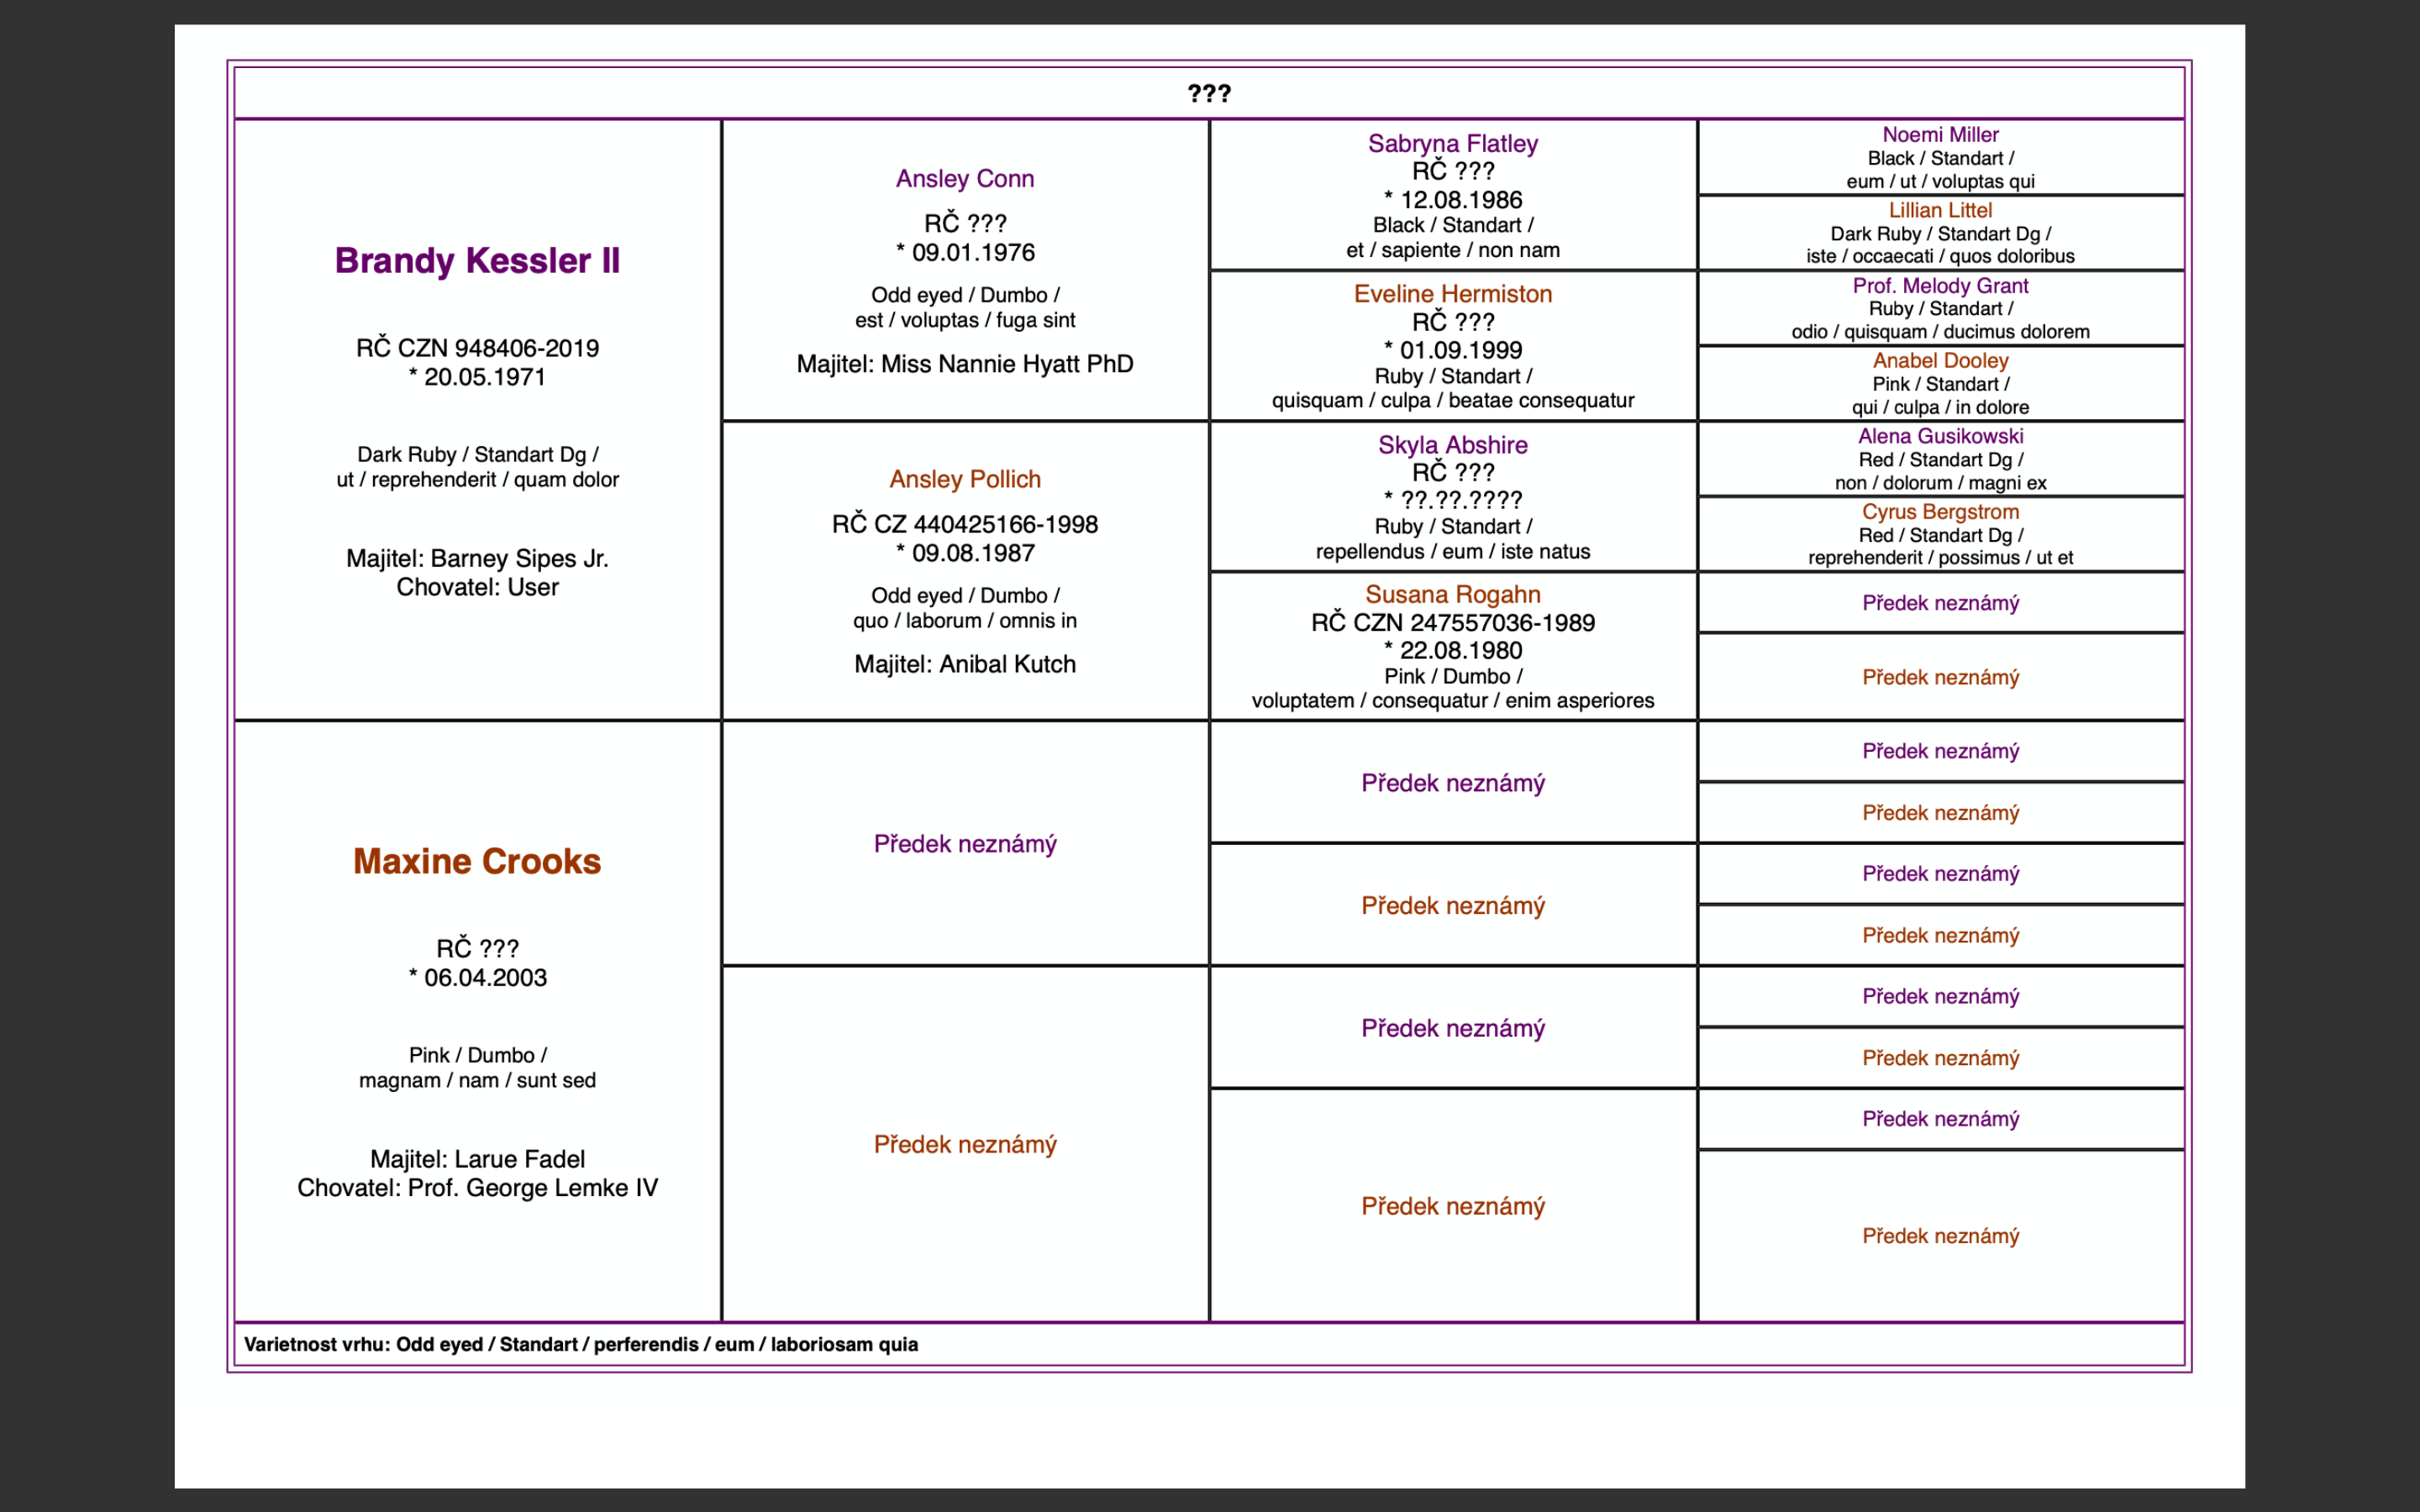
\includegraphics[width=1.0\textwidth]{media/priloha/vseobecne/pdf/2.png}
	\caption{Screenshot zobrazujúci druhú stranu vygenerovaného PDF súbor zvieraťa}
\end{figure}

\begin{figure}[H]
	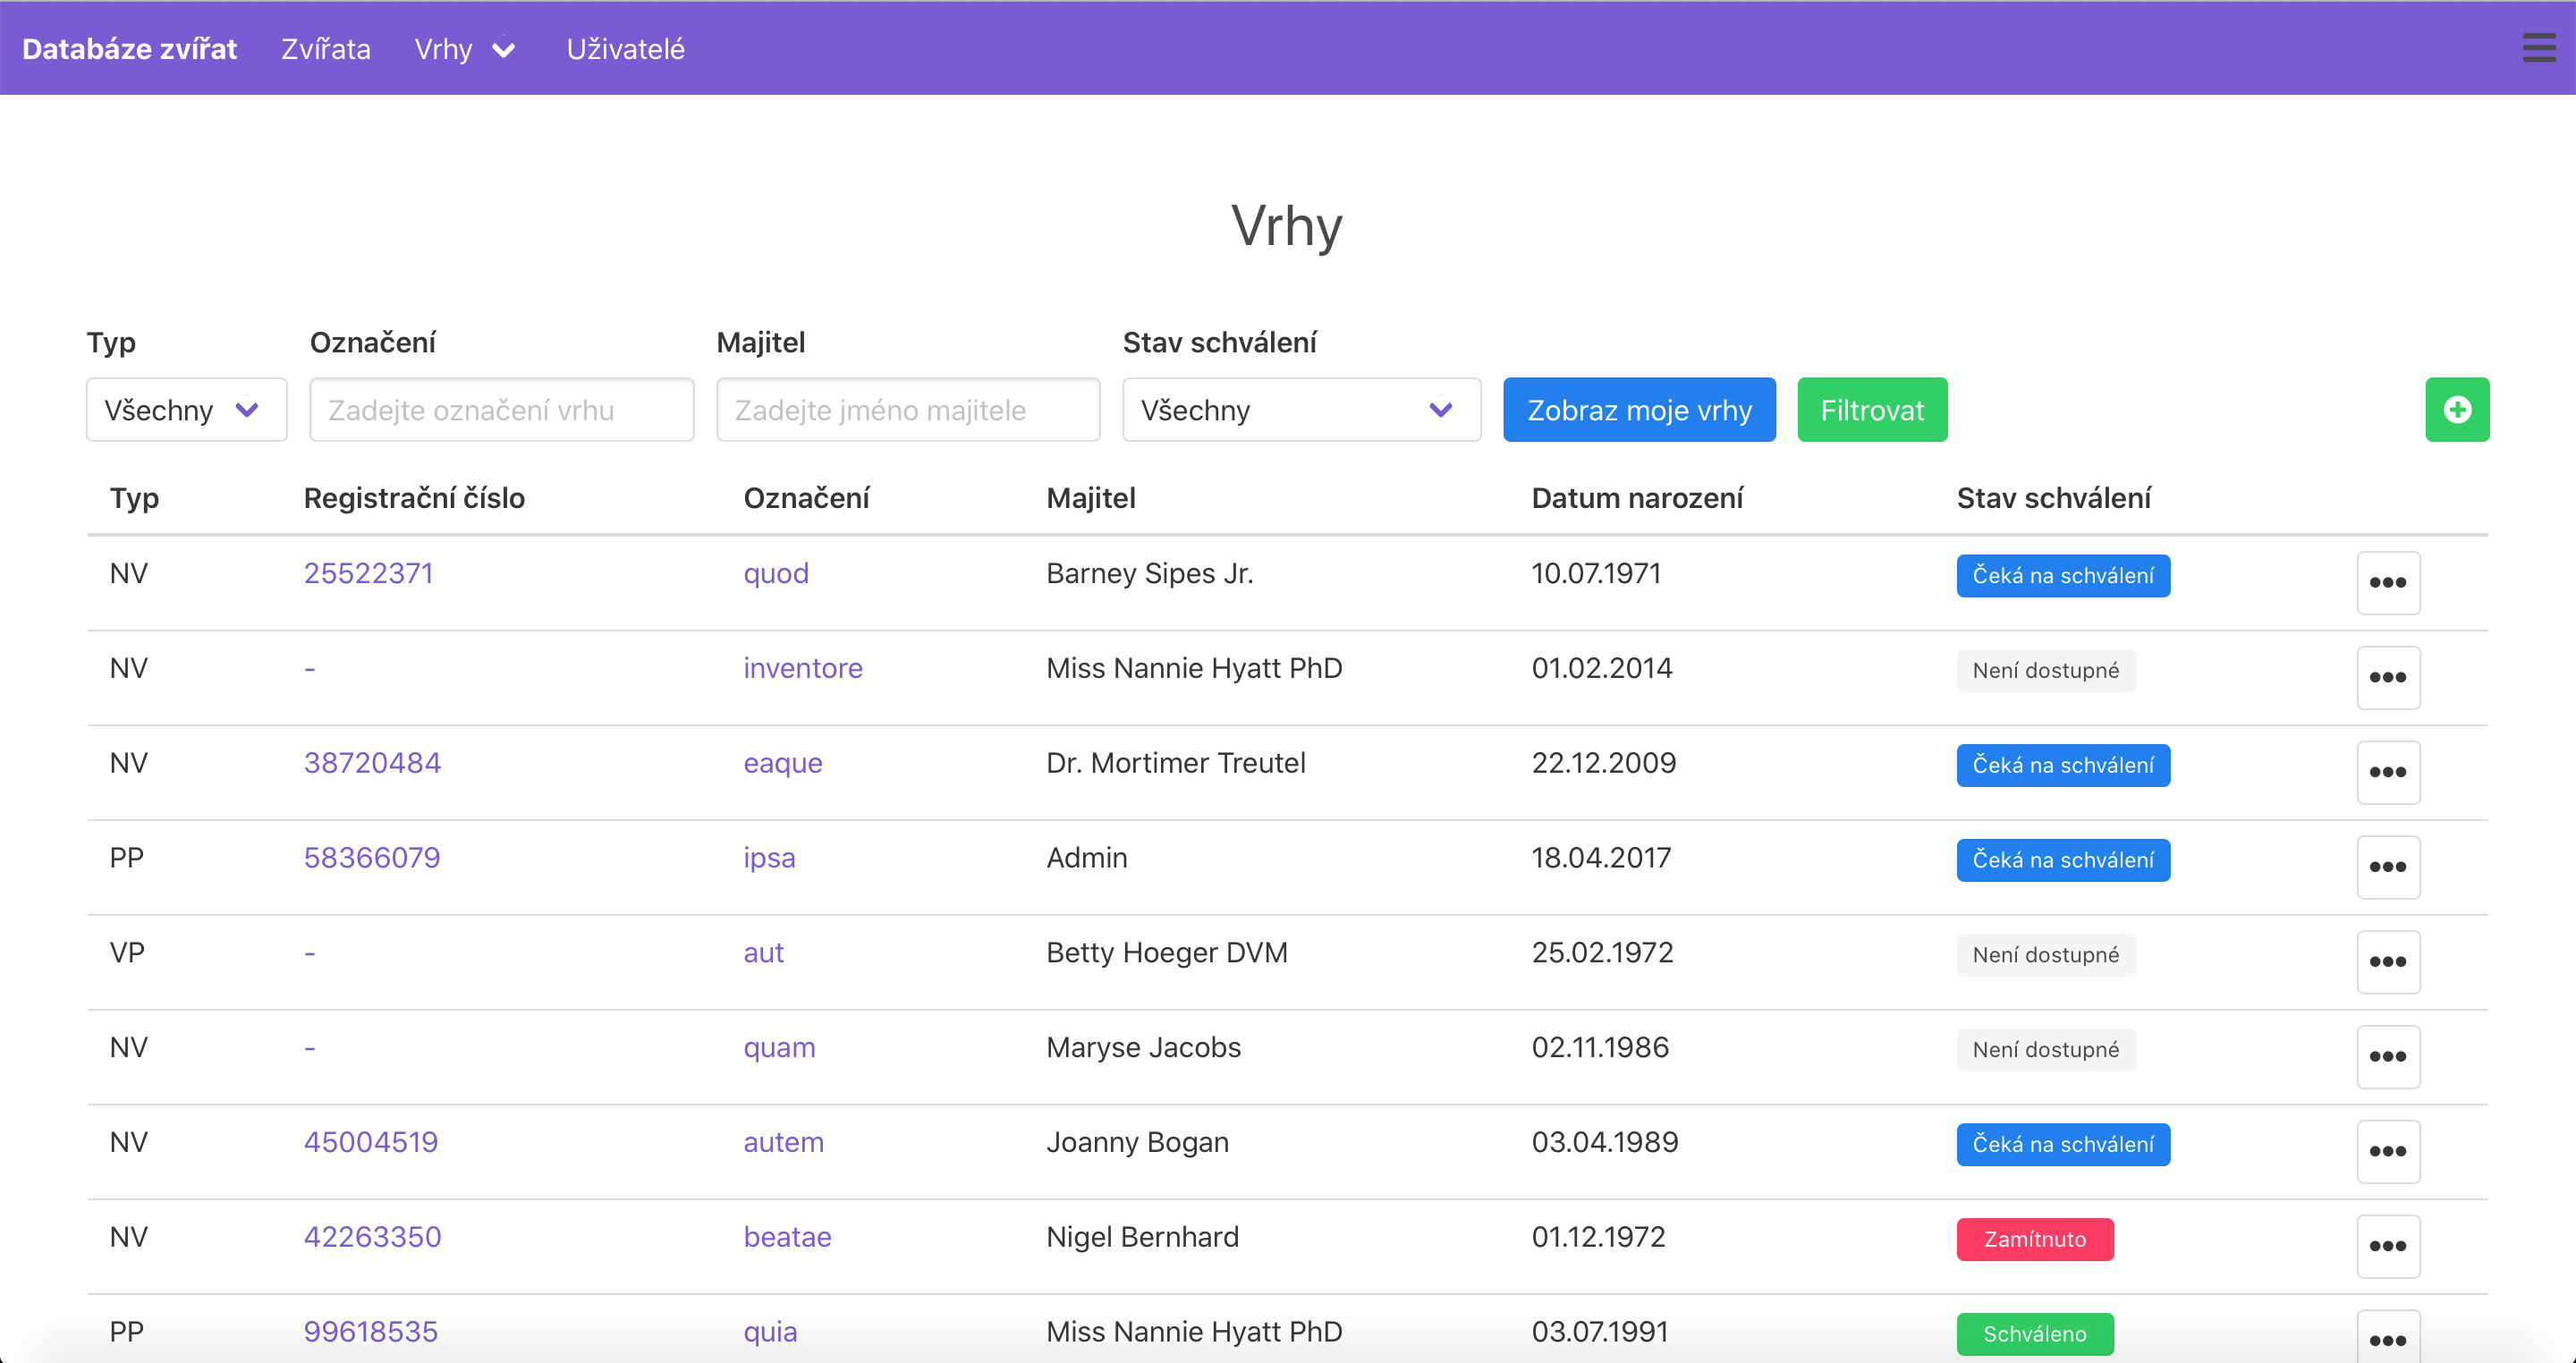
\includegraphics[width=1.0\textwidth]{media/priloha/vrhy/1.png}
	\caption{Screenshot zobrazujúci tabuľku všetkých vrhov}
\end{figure}

\vspace*{\fill}

\begin{figure}[H]
	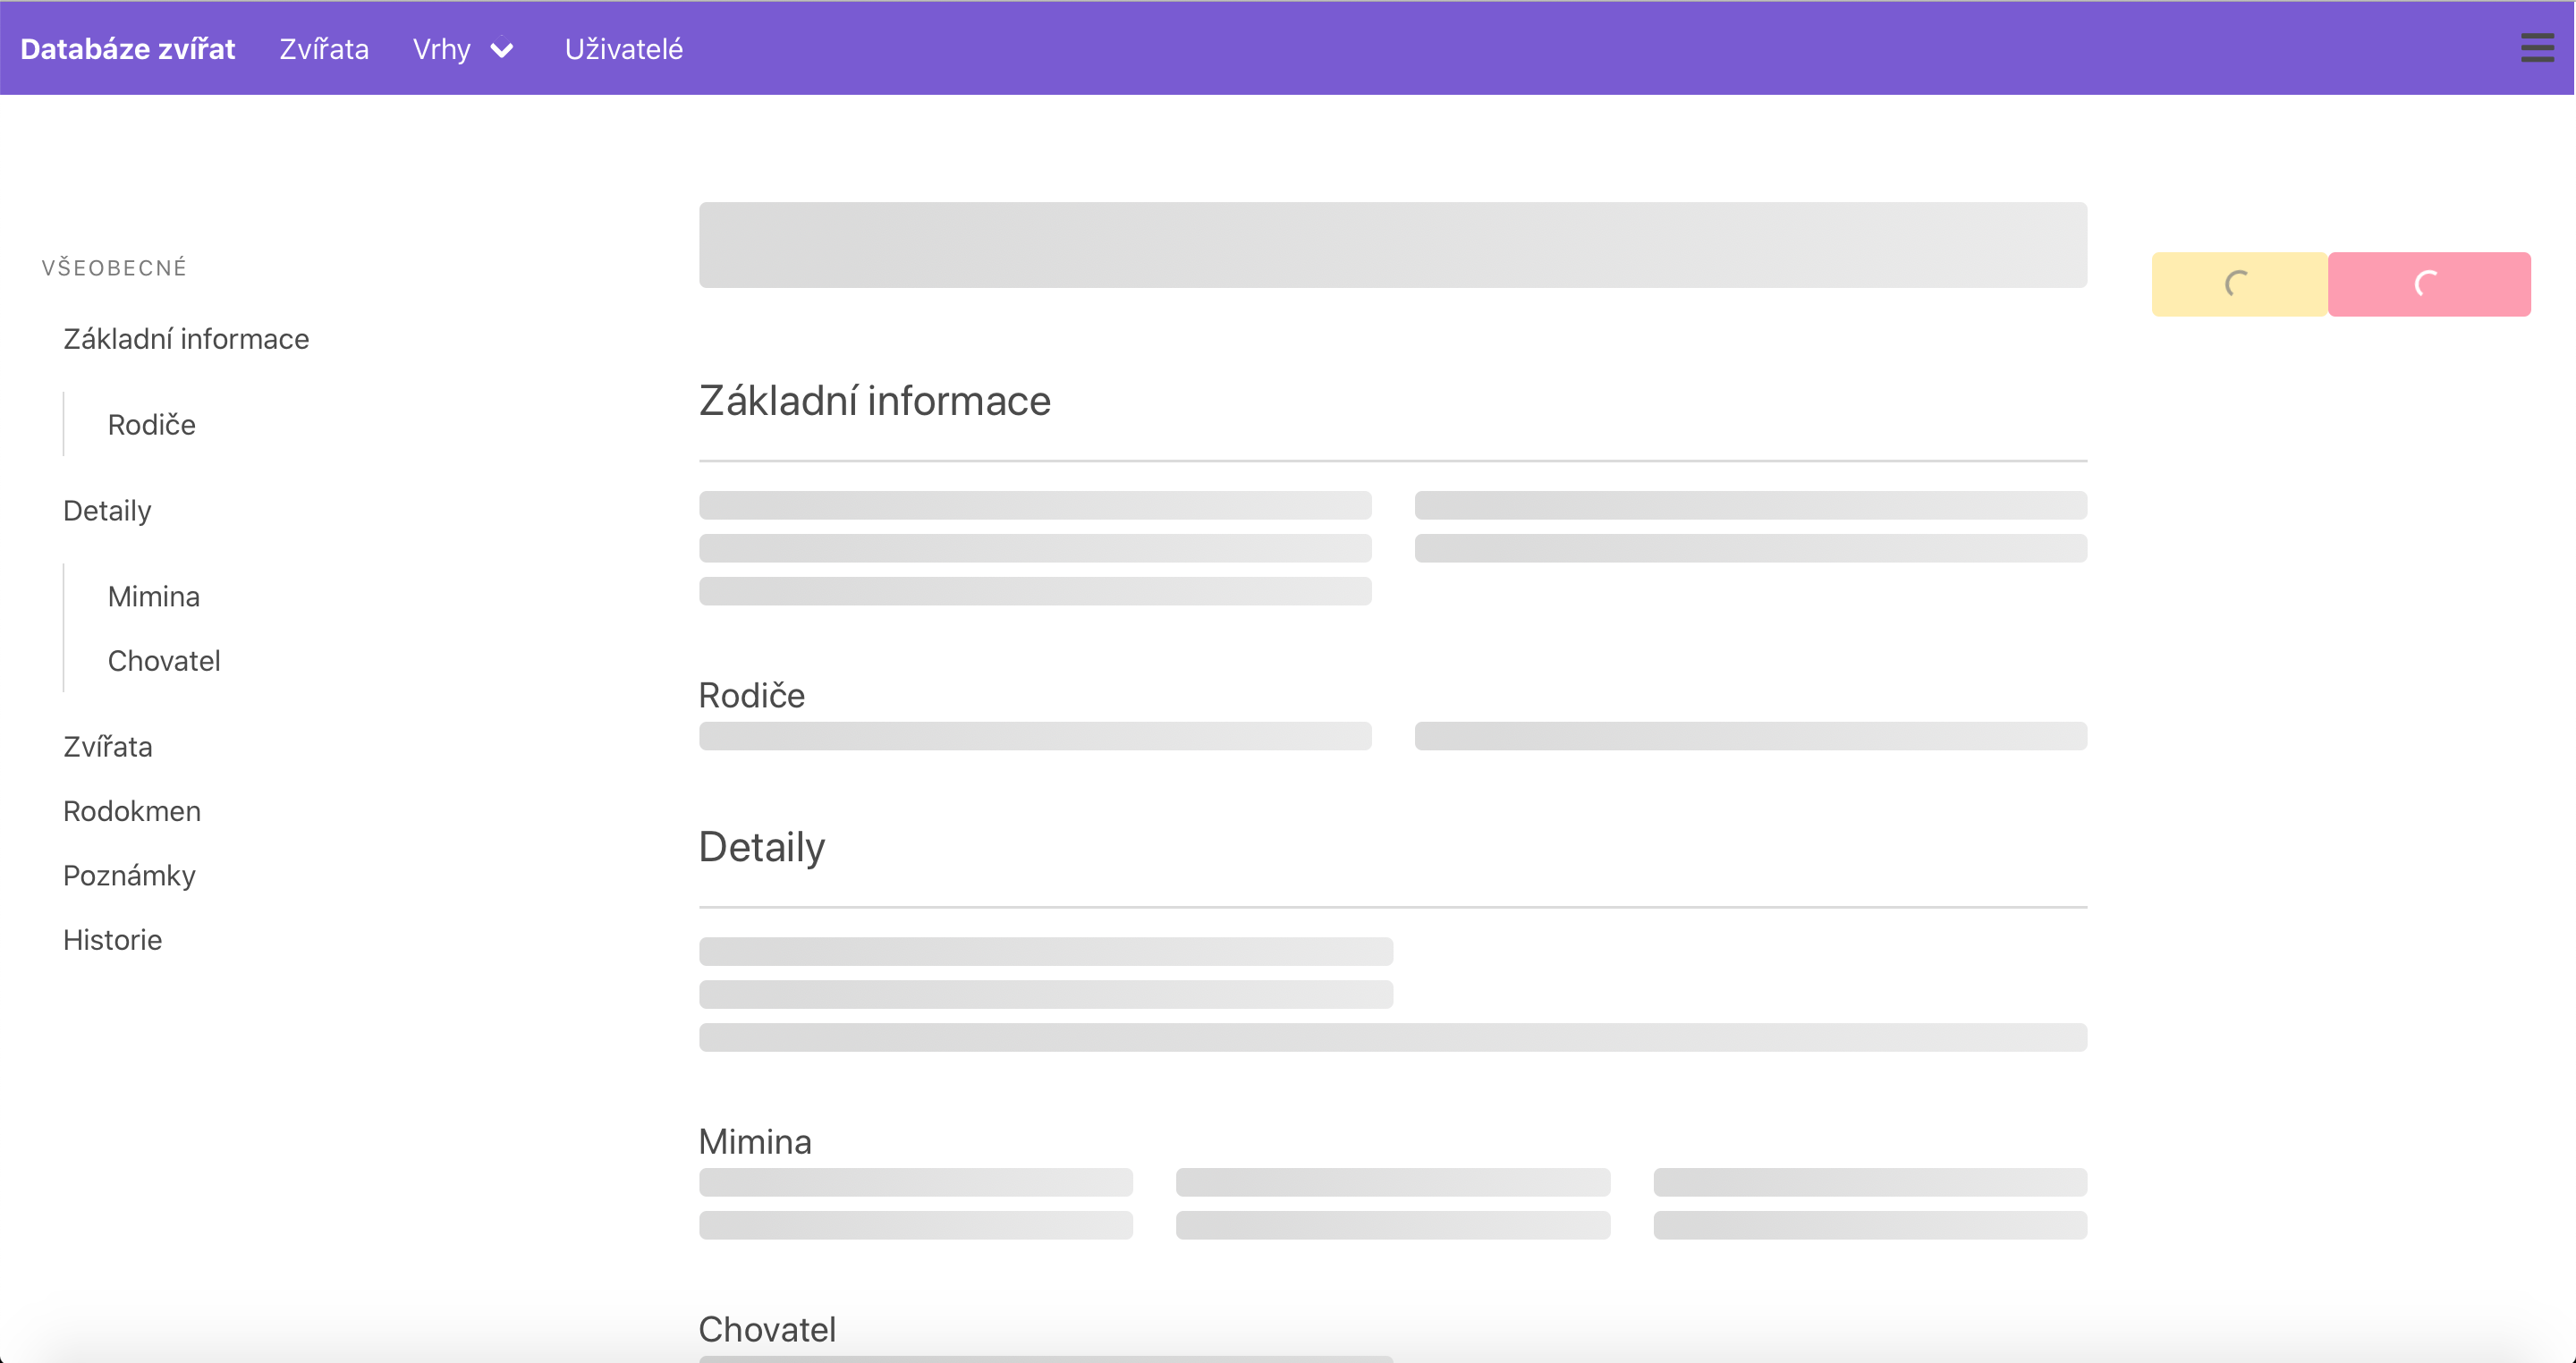
\includegraphics[width=1.0\textwidth]{media/priloha/vrh/1.png}
	\caption{Screenshot aplikácie zobrazujúci načítavanie zvoleného vrhu}
\end{figure}

\begin{figure}[H]
	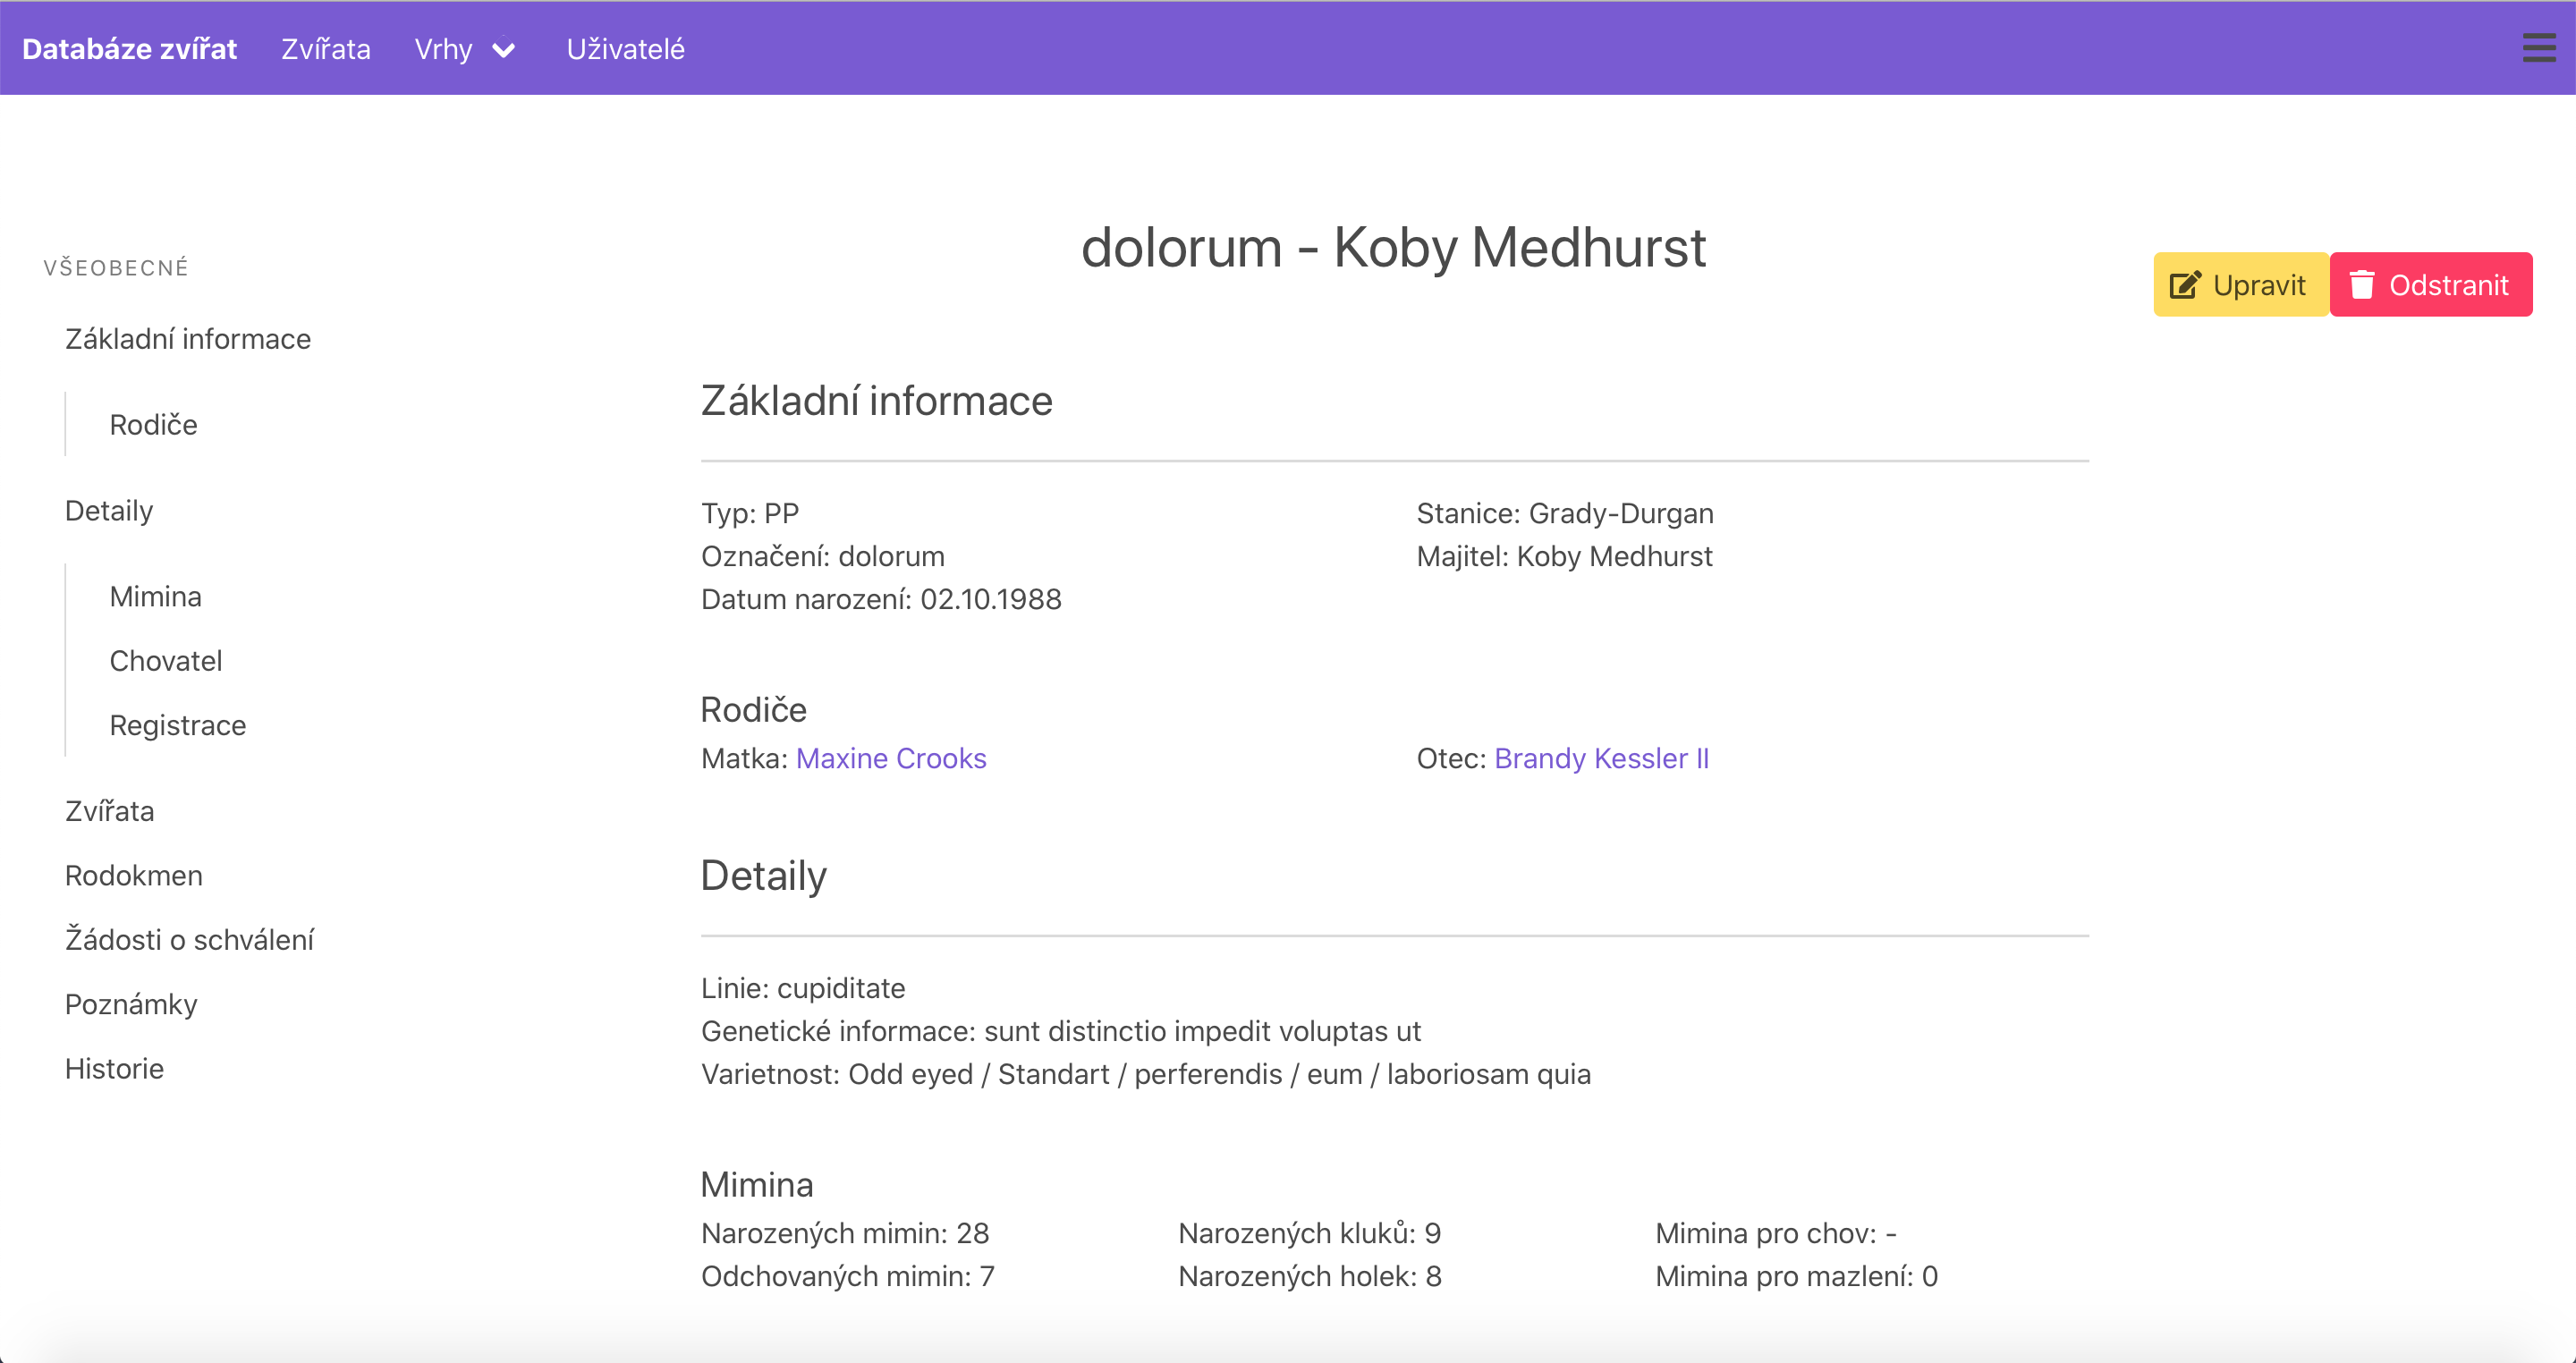
\includegraphics[width=1.0\textwidth]{media/priloha/vrh/2.png}
	\caption{Screenshot aplikácie zobrazujúci načítaný vrh}
\end{figure}

\vspace*{\fill}

\begin{figure}[H]
	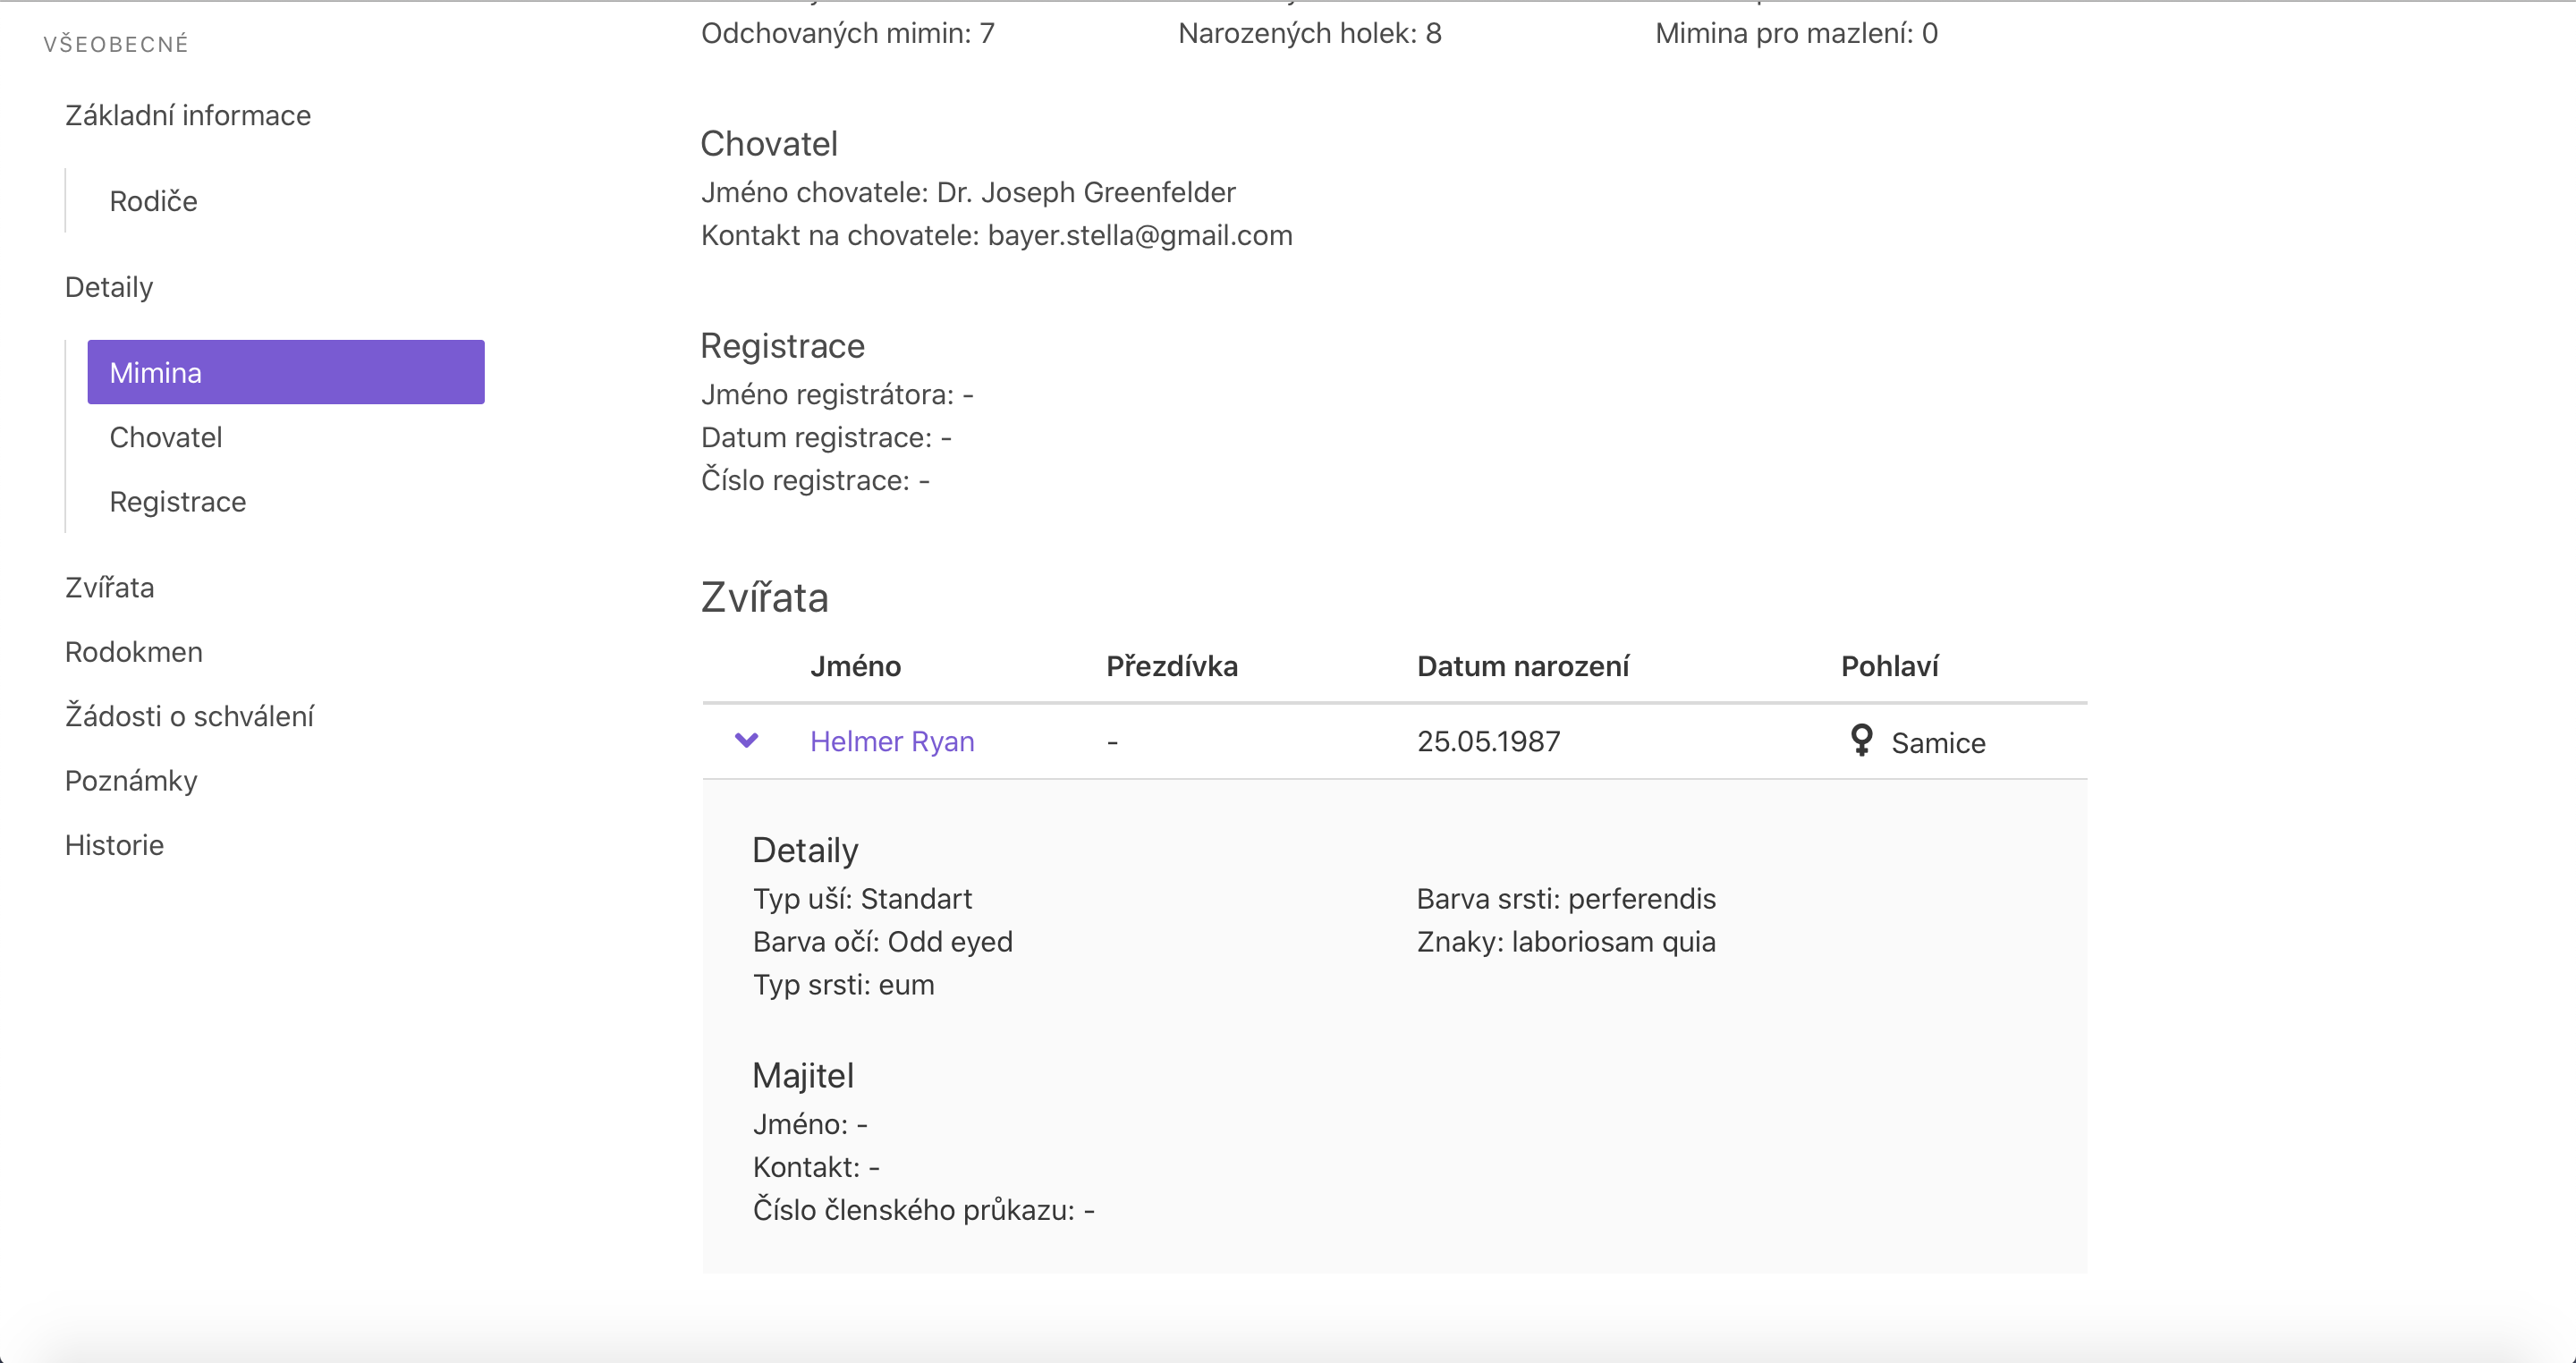
\includegraphics[width=1.0\textwidth]{media/priloha/vrh/3.png}
	\caption{Screenshot aplikácie zobrazujúci dodatočné informácie o vrhu}
\end{figure}

\begin{figure}[H]
	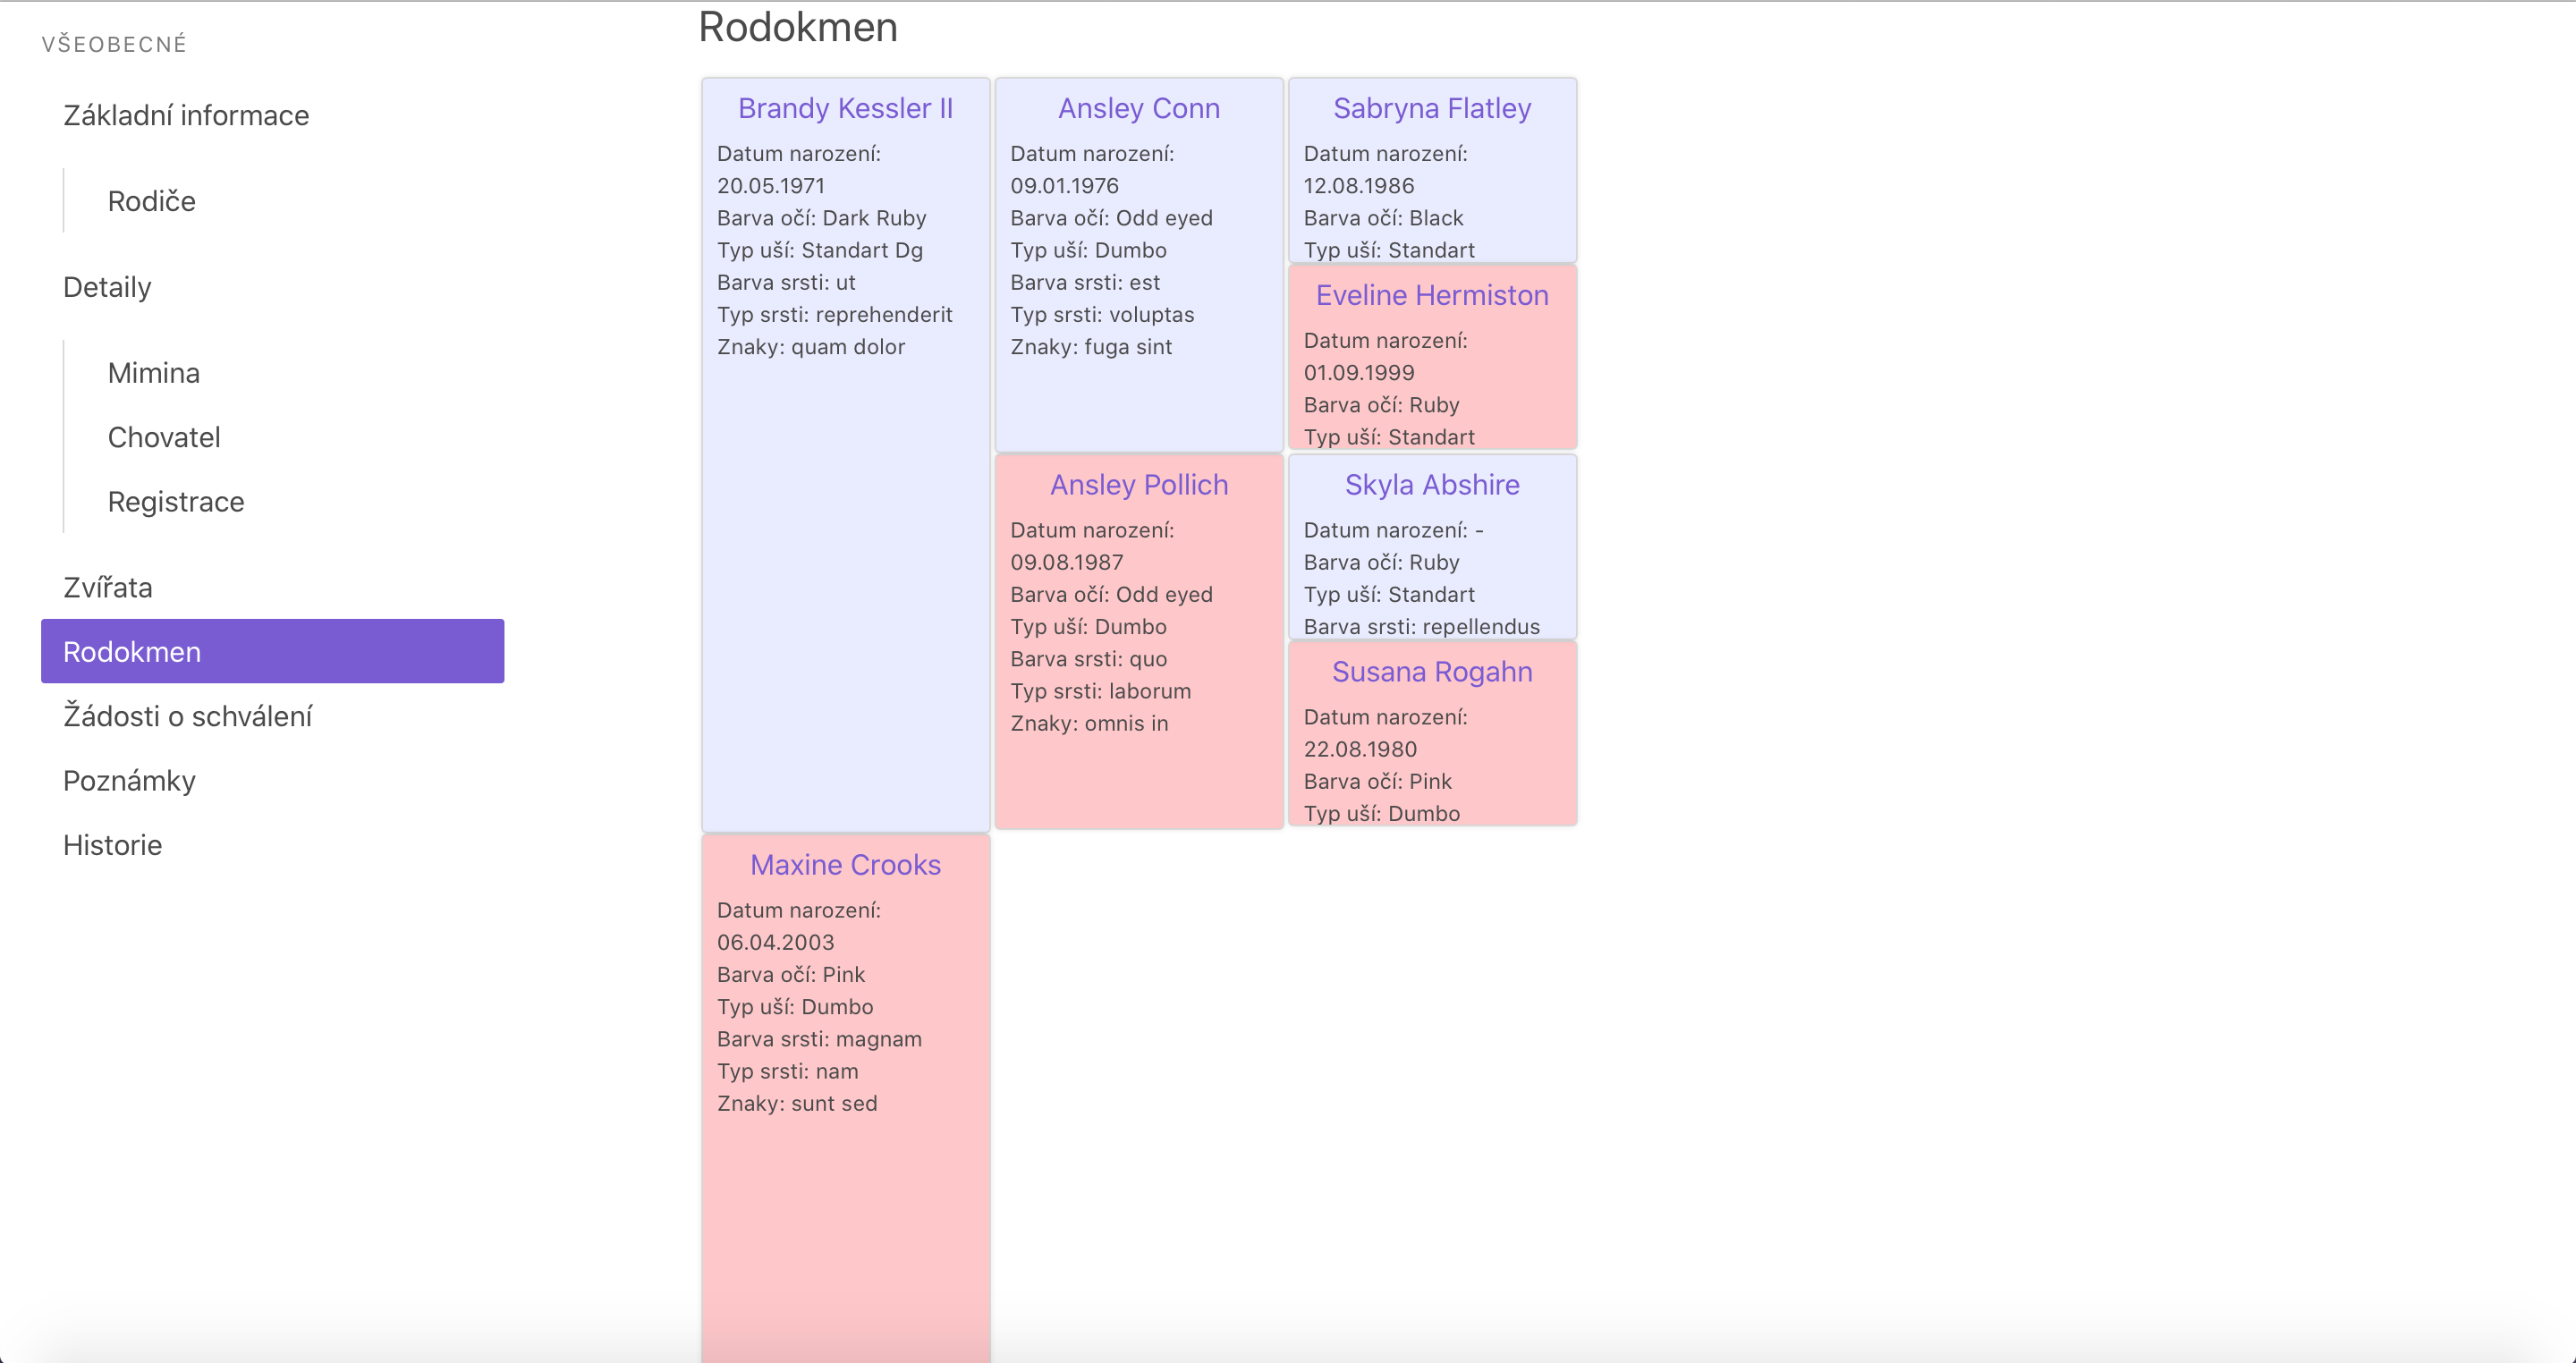
\includegraphics[width=1.0\textwidth]{media/priloha/vrh/4.png}
	\caption{Screenshot aplikácie zobrazujúci rodokmeň vrhu}
\end{figure}

\vspace*{\fill}

\begin{figure}[H]
	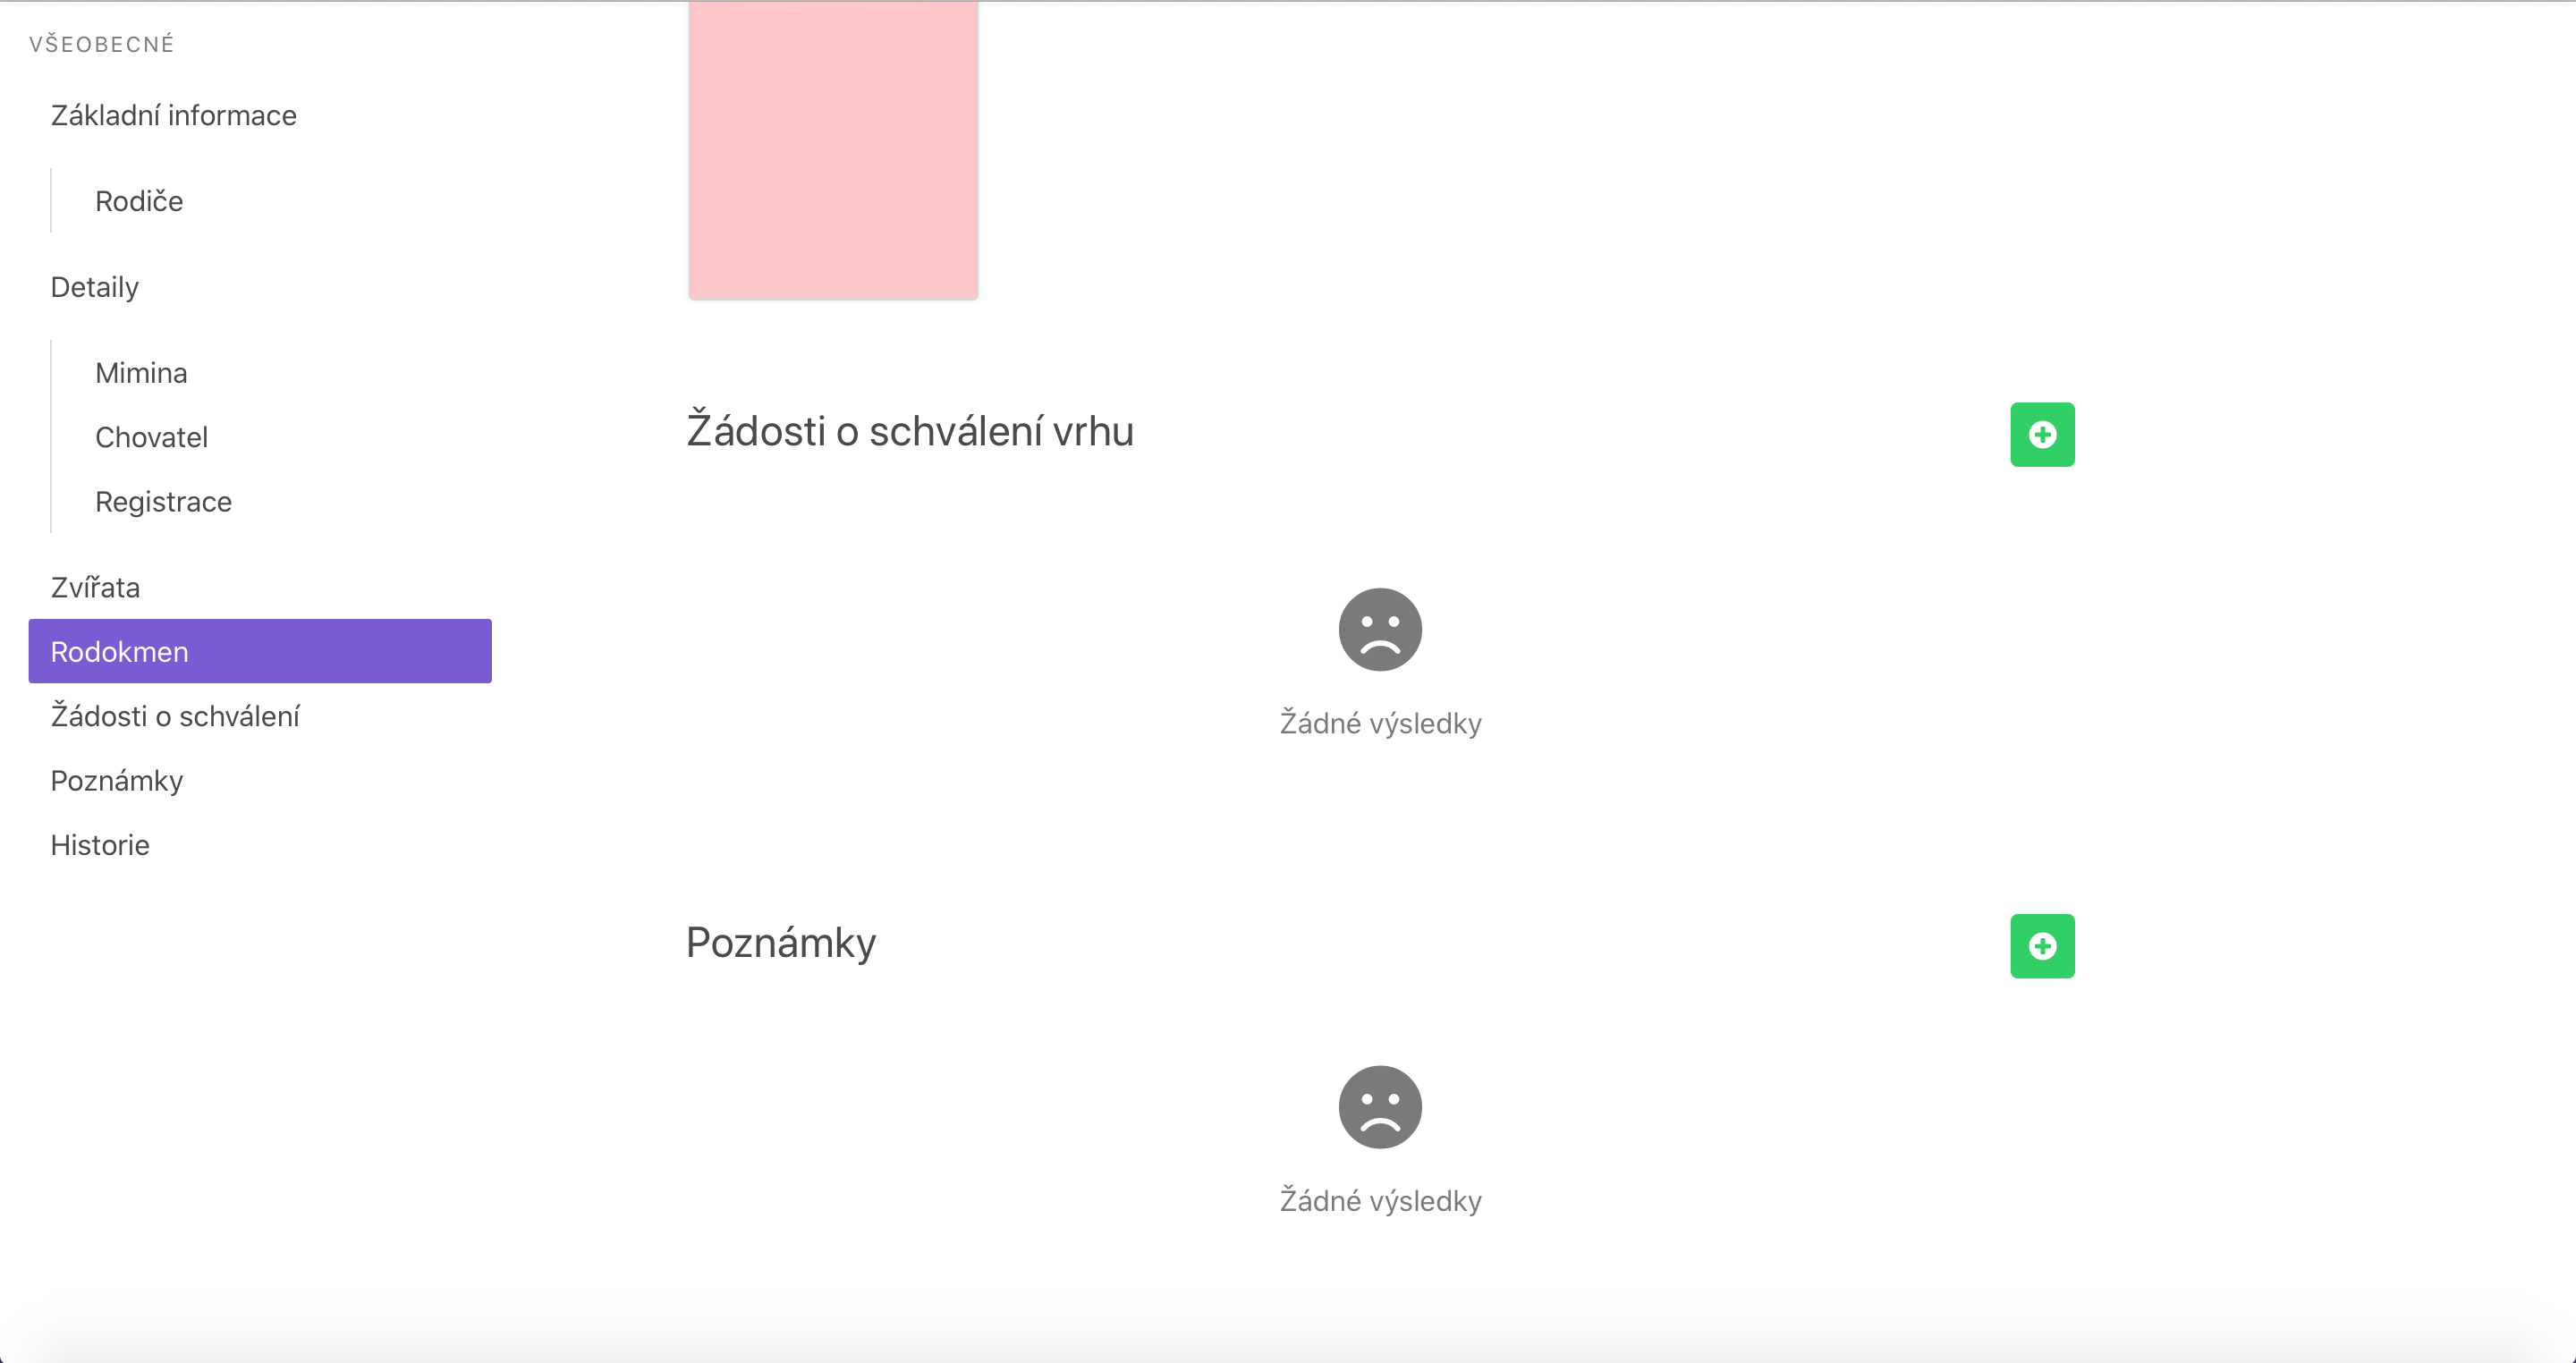
\includegraphics[width=1.0\textwidth]{media/priloha/vrh/5.png}
	\caption{Screenshot aplikácie zobrazujúci ďaľšiu sekciu informácií o vrhu}
\end{figure}

\begin{figure}[H]
	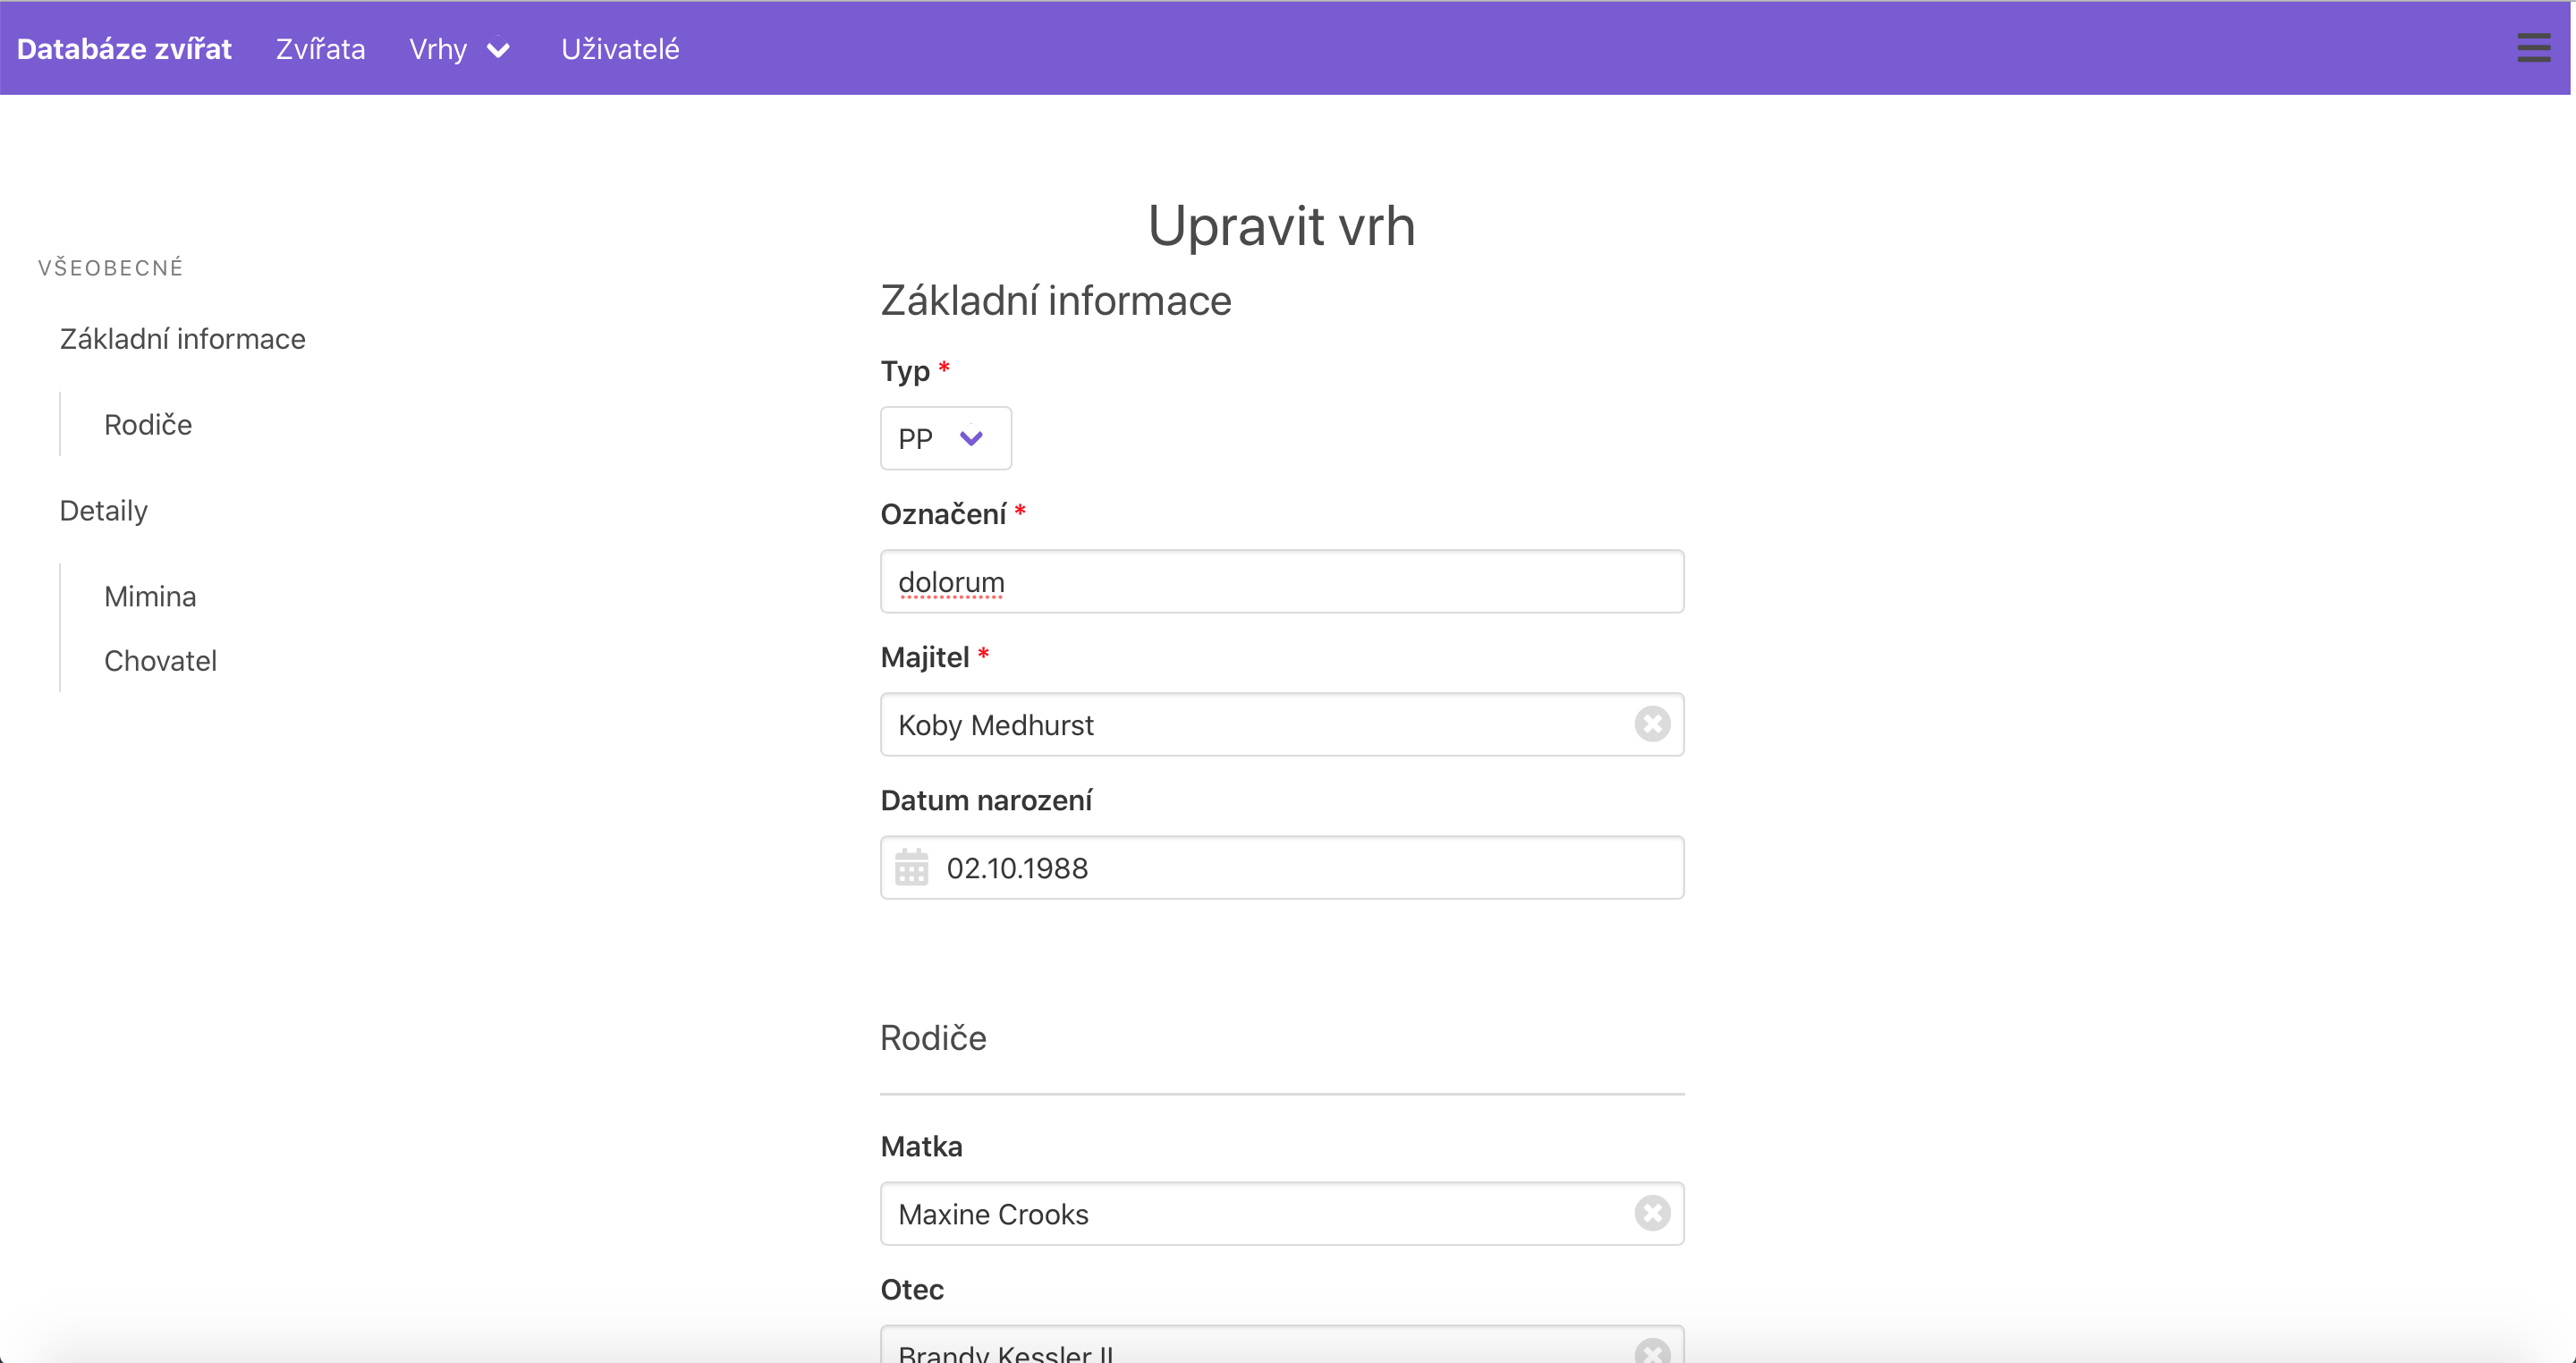
\includegraphics[width=1.0\textwidth]{media/priloha/vrh/editacia/1.png}
	\caption{Screenshot aplikácie zobrazujúci sekciu editácie vrhu}
\end{figure}

\vspace*{\fill}

\begin{figure}[H]
	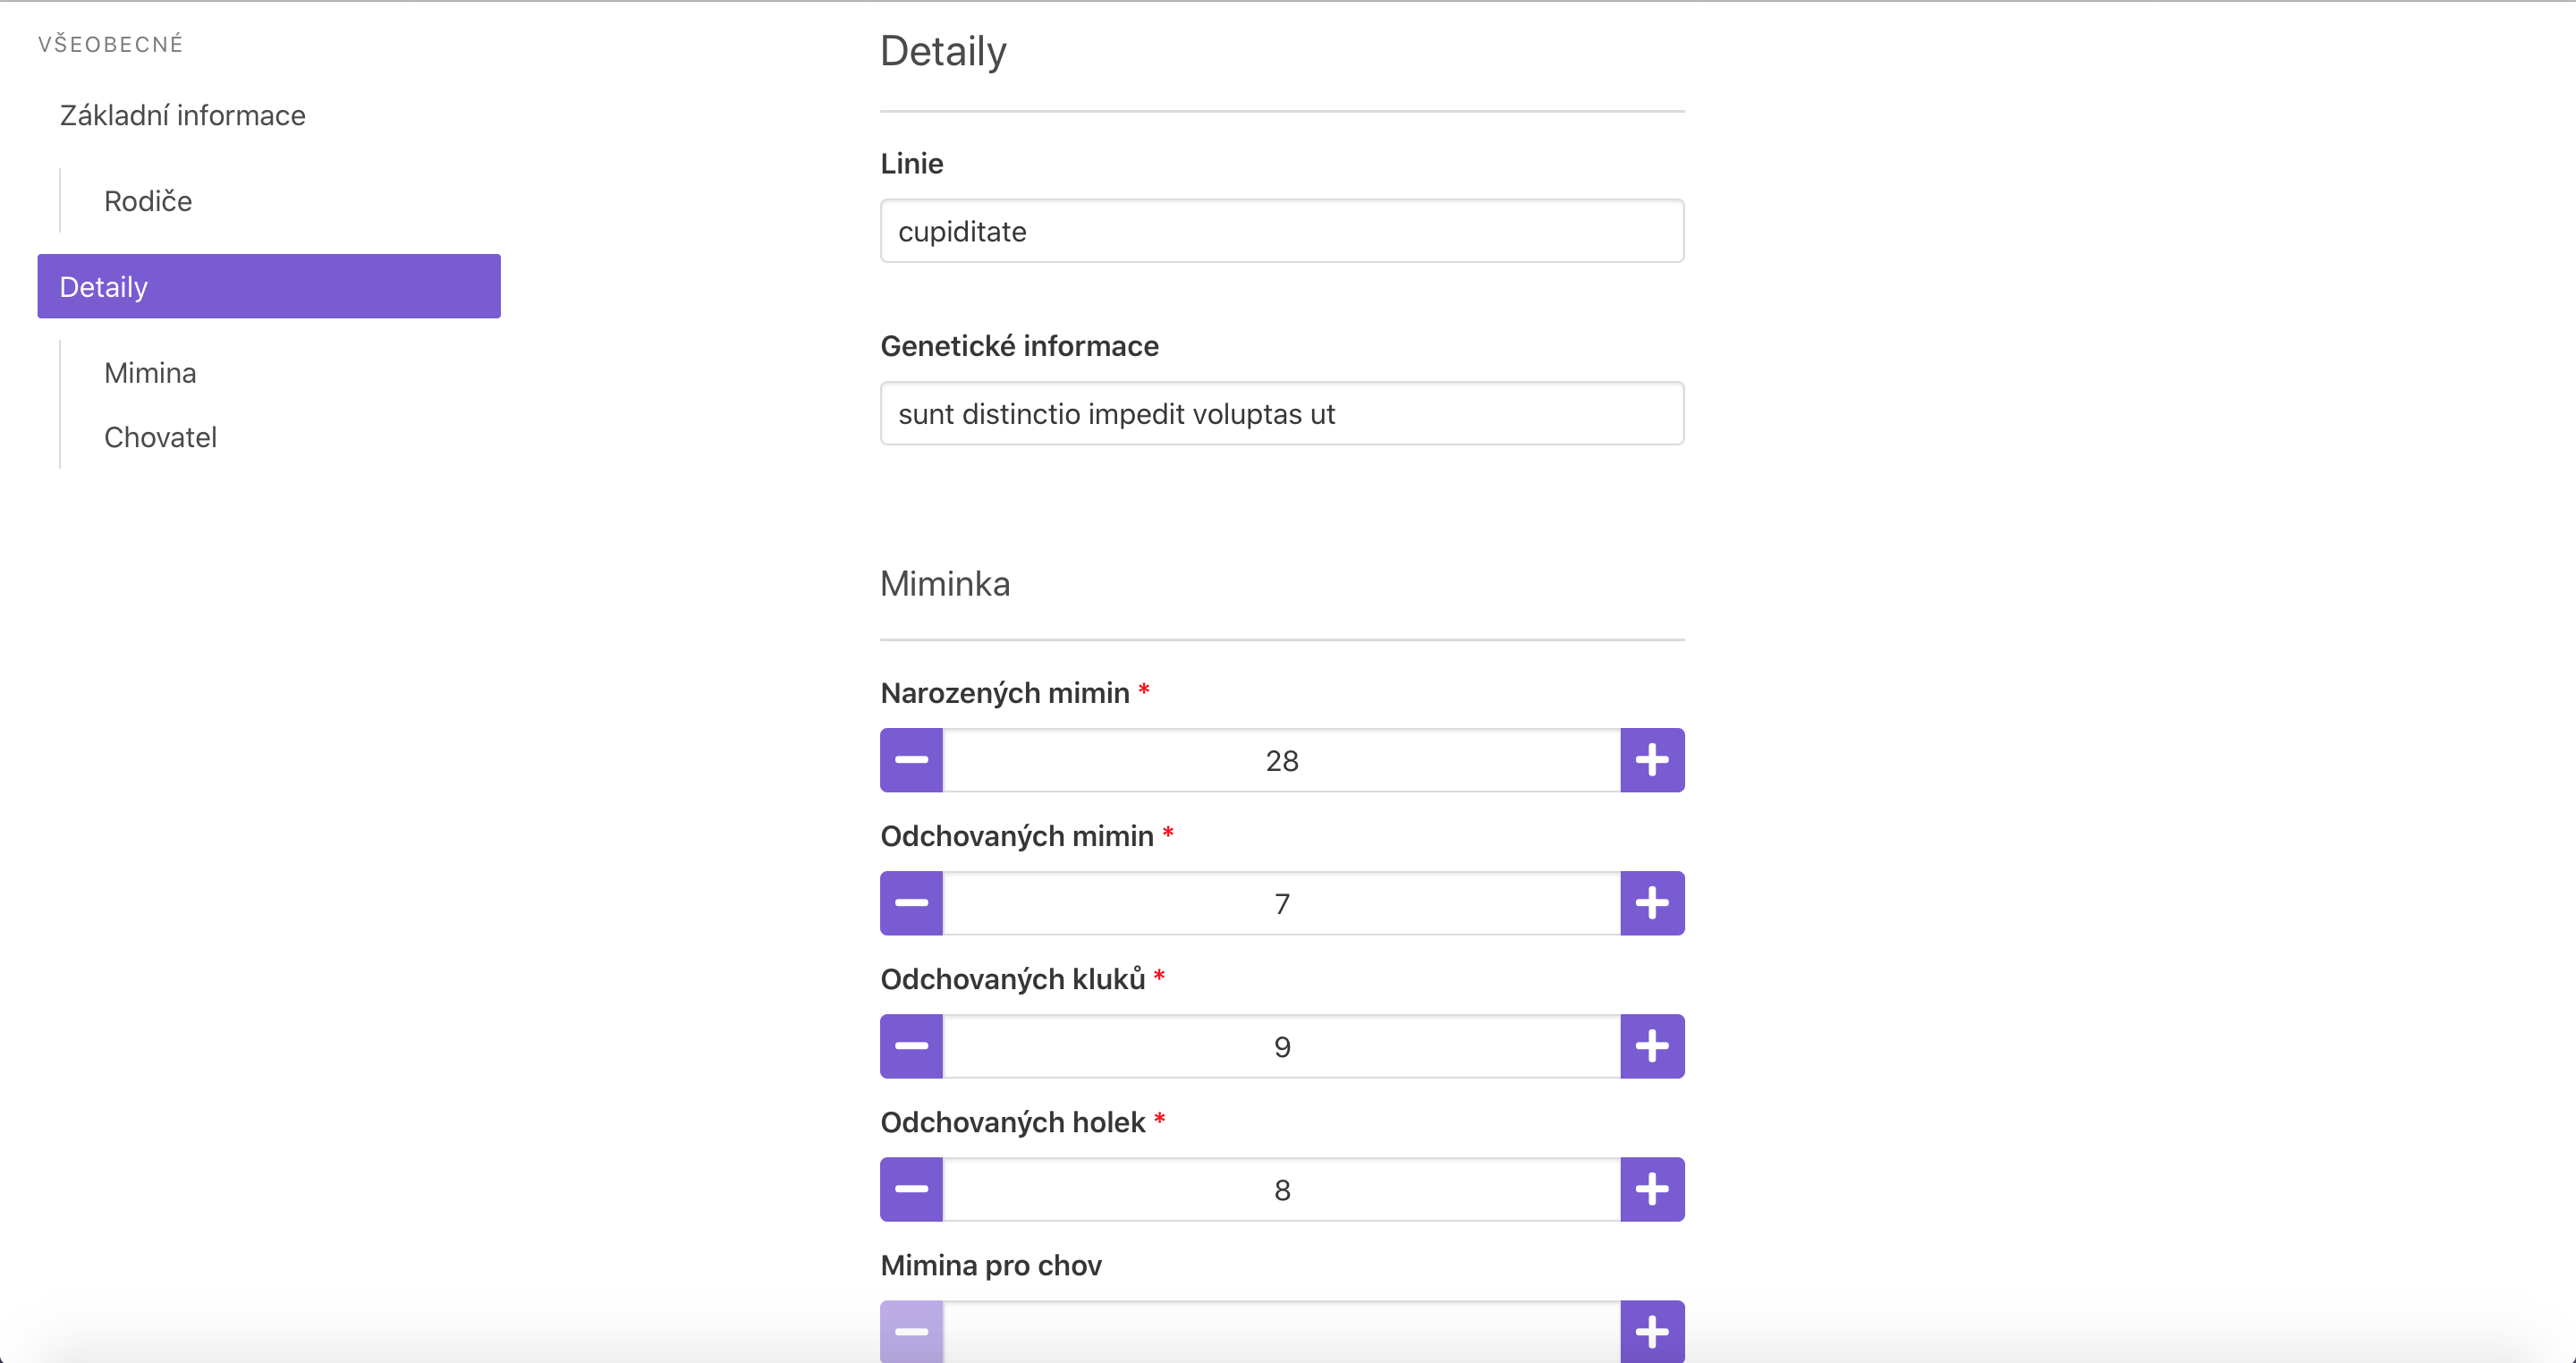
\includegraphics[width=1.0\textwidth]{media/priloha/vrh/editacia/2.png}
	\caption{Screenshot aplikácie zobrazujúci ďaľšiu sekciu informácií o vrhu}
\end{figure}

\begin{figure}[H]
	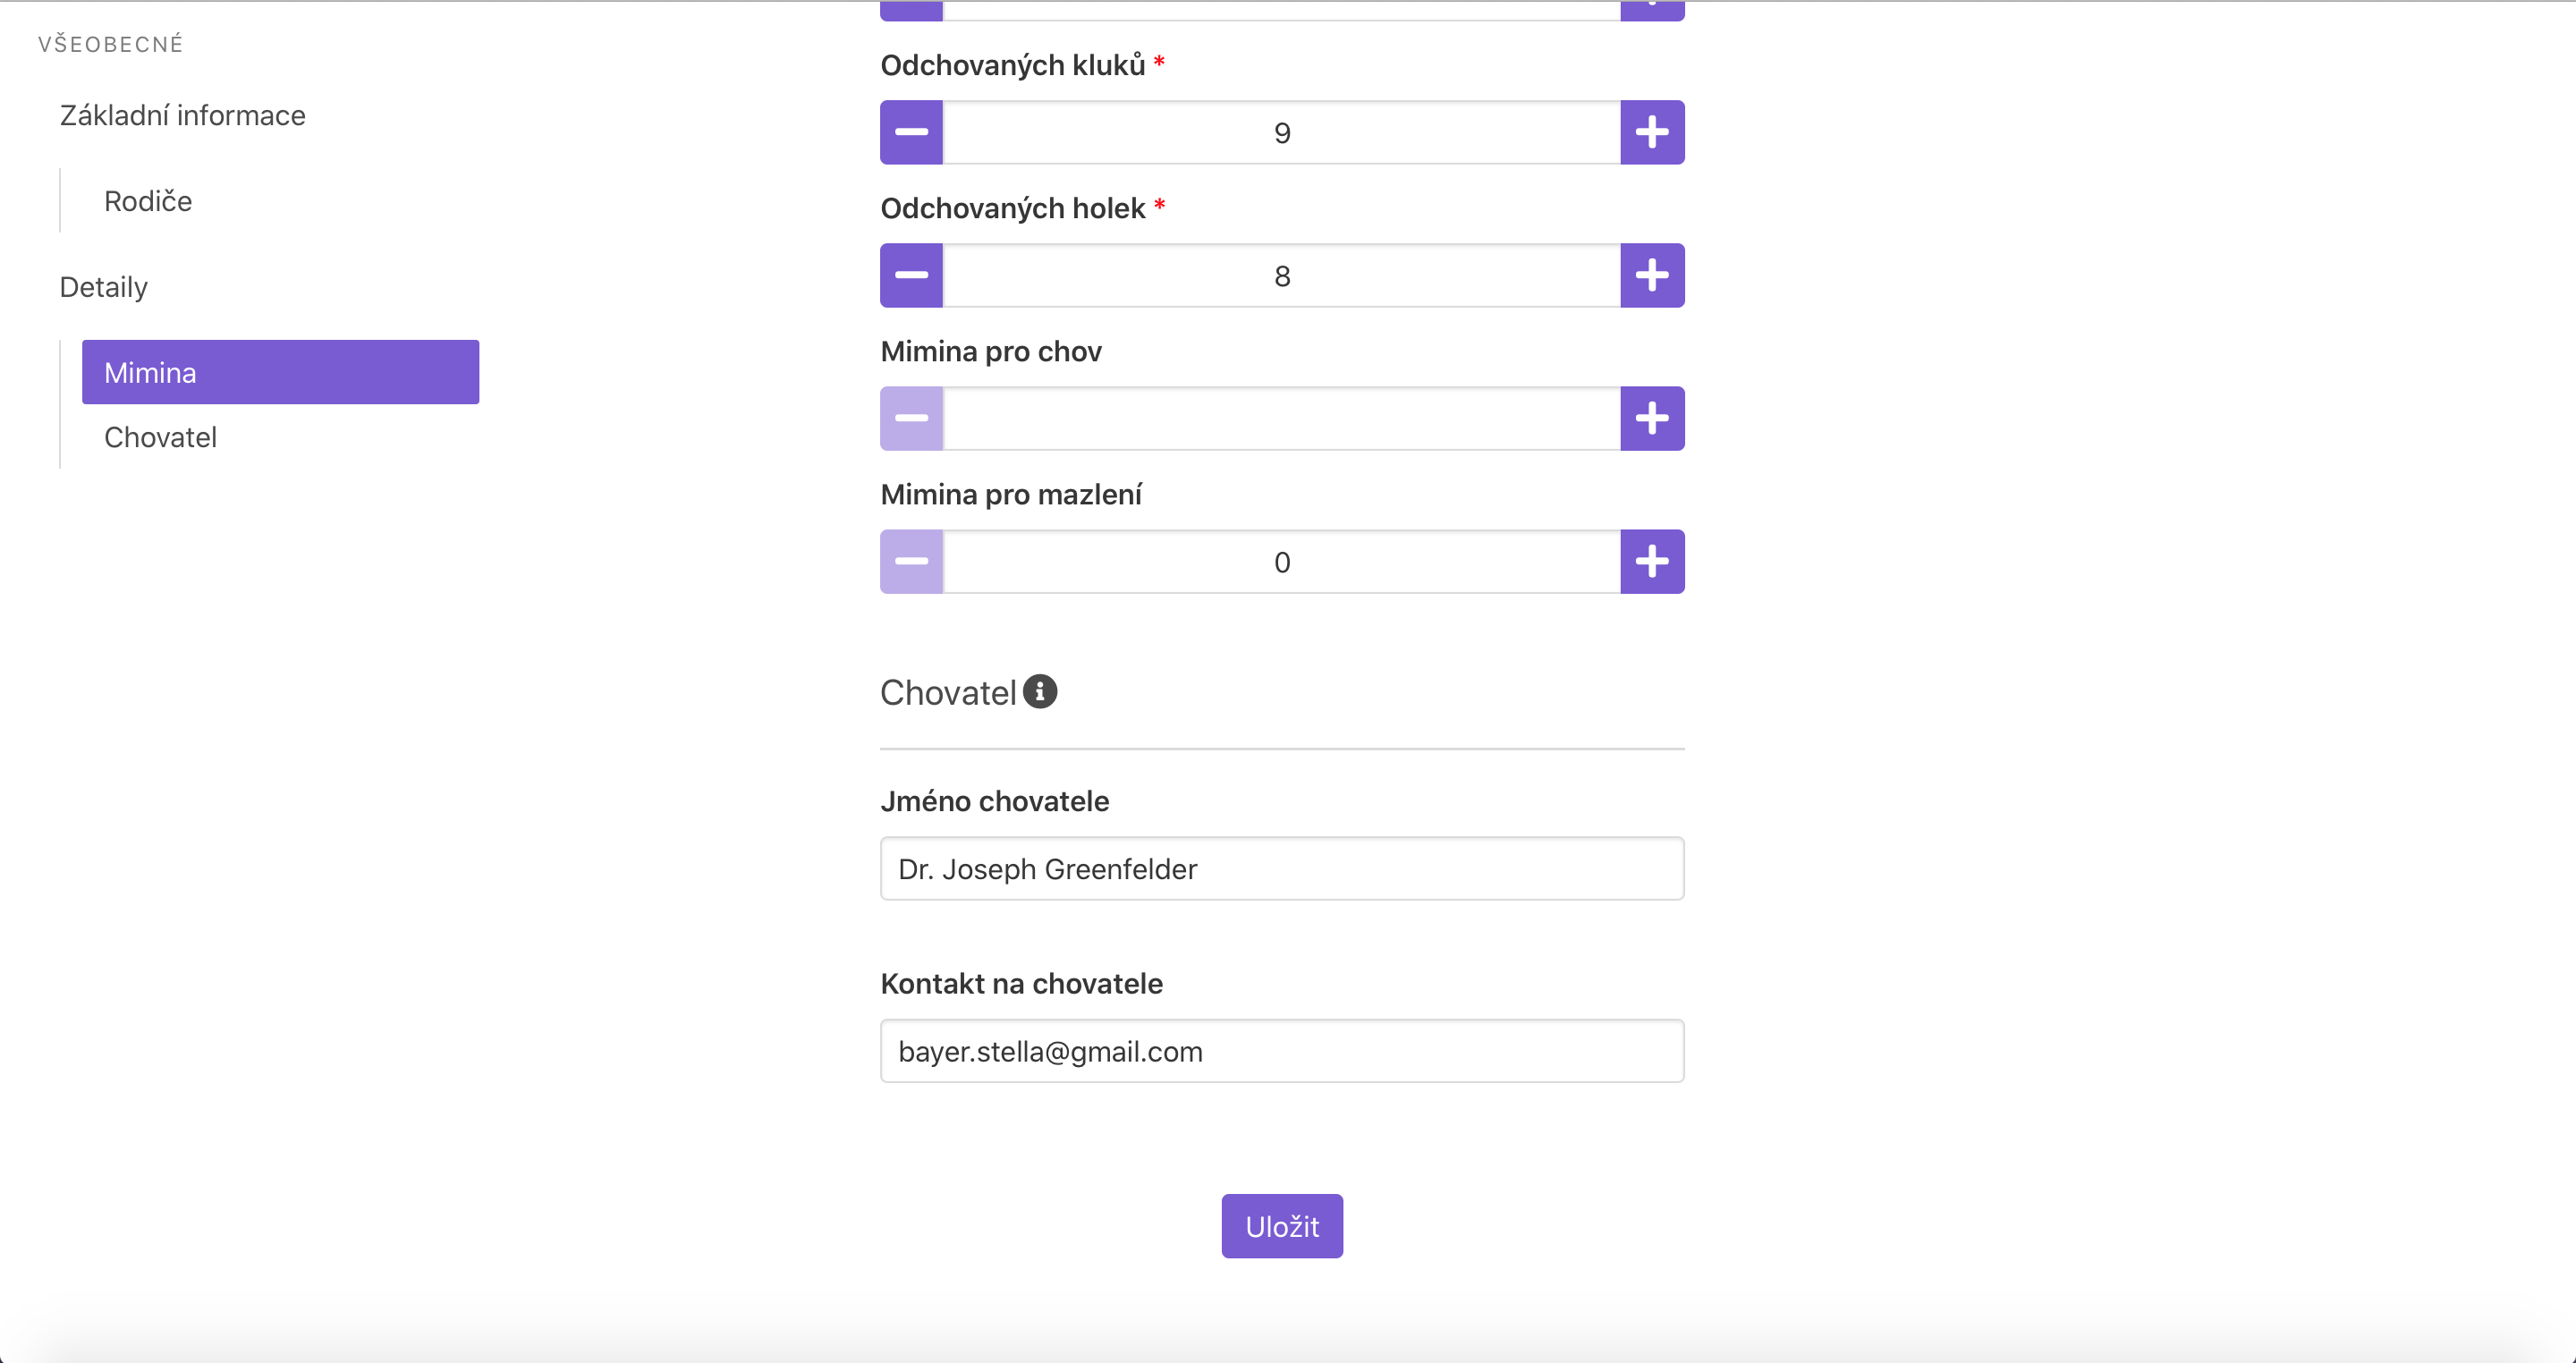
\includegraphics[width=1.0\textwidth]{media/priloha/vrh/editacia/3.png}
	\caption{Screenshot aplikácie zobrazujúci poslednú sekciu editácie vrhu}
\end{figure}

\vspace*{\fill}

\begin{figure}[H]
	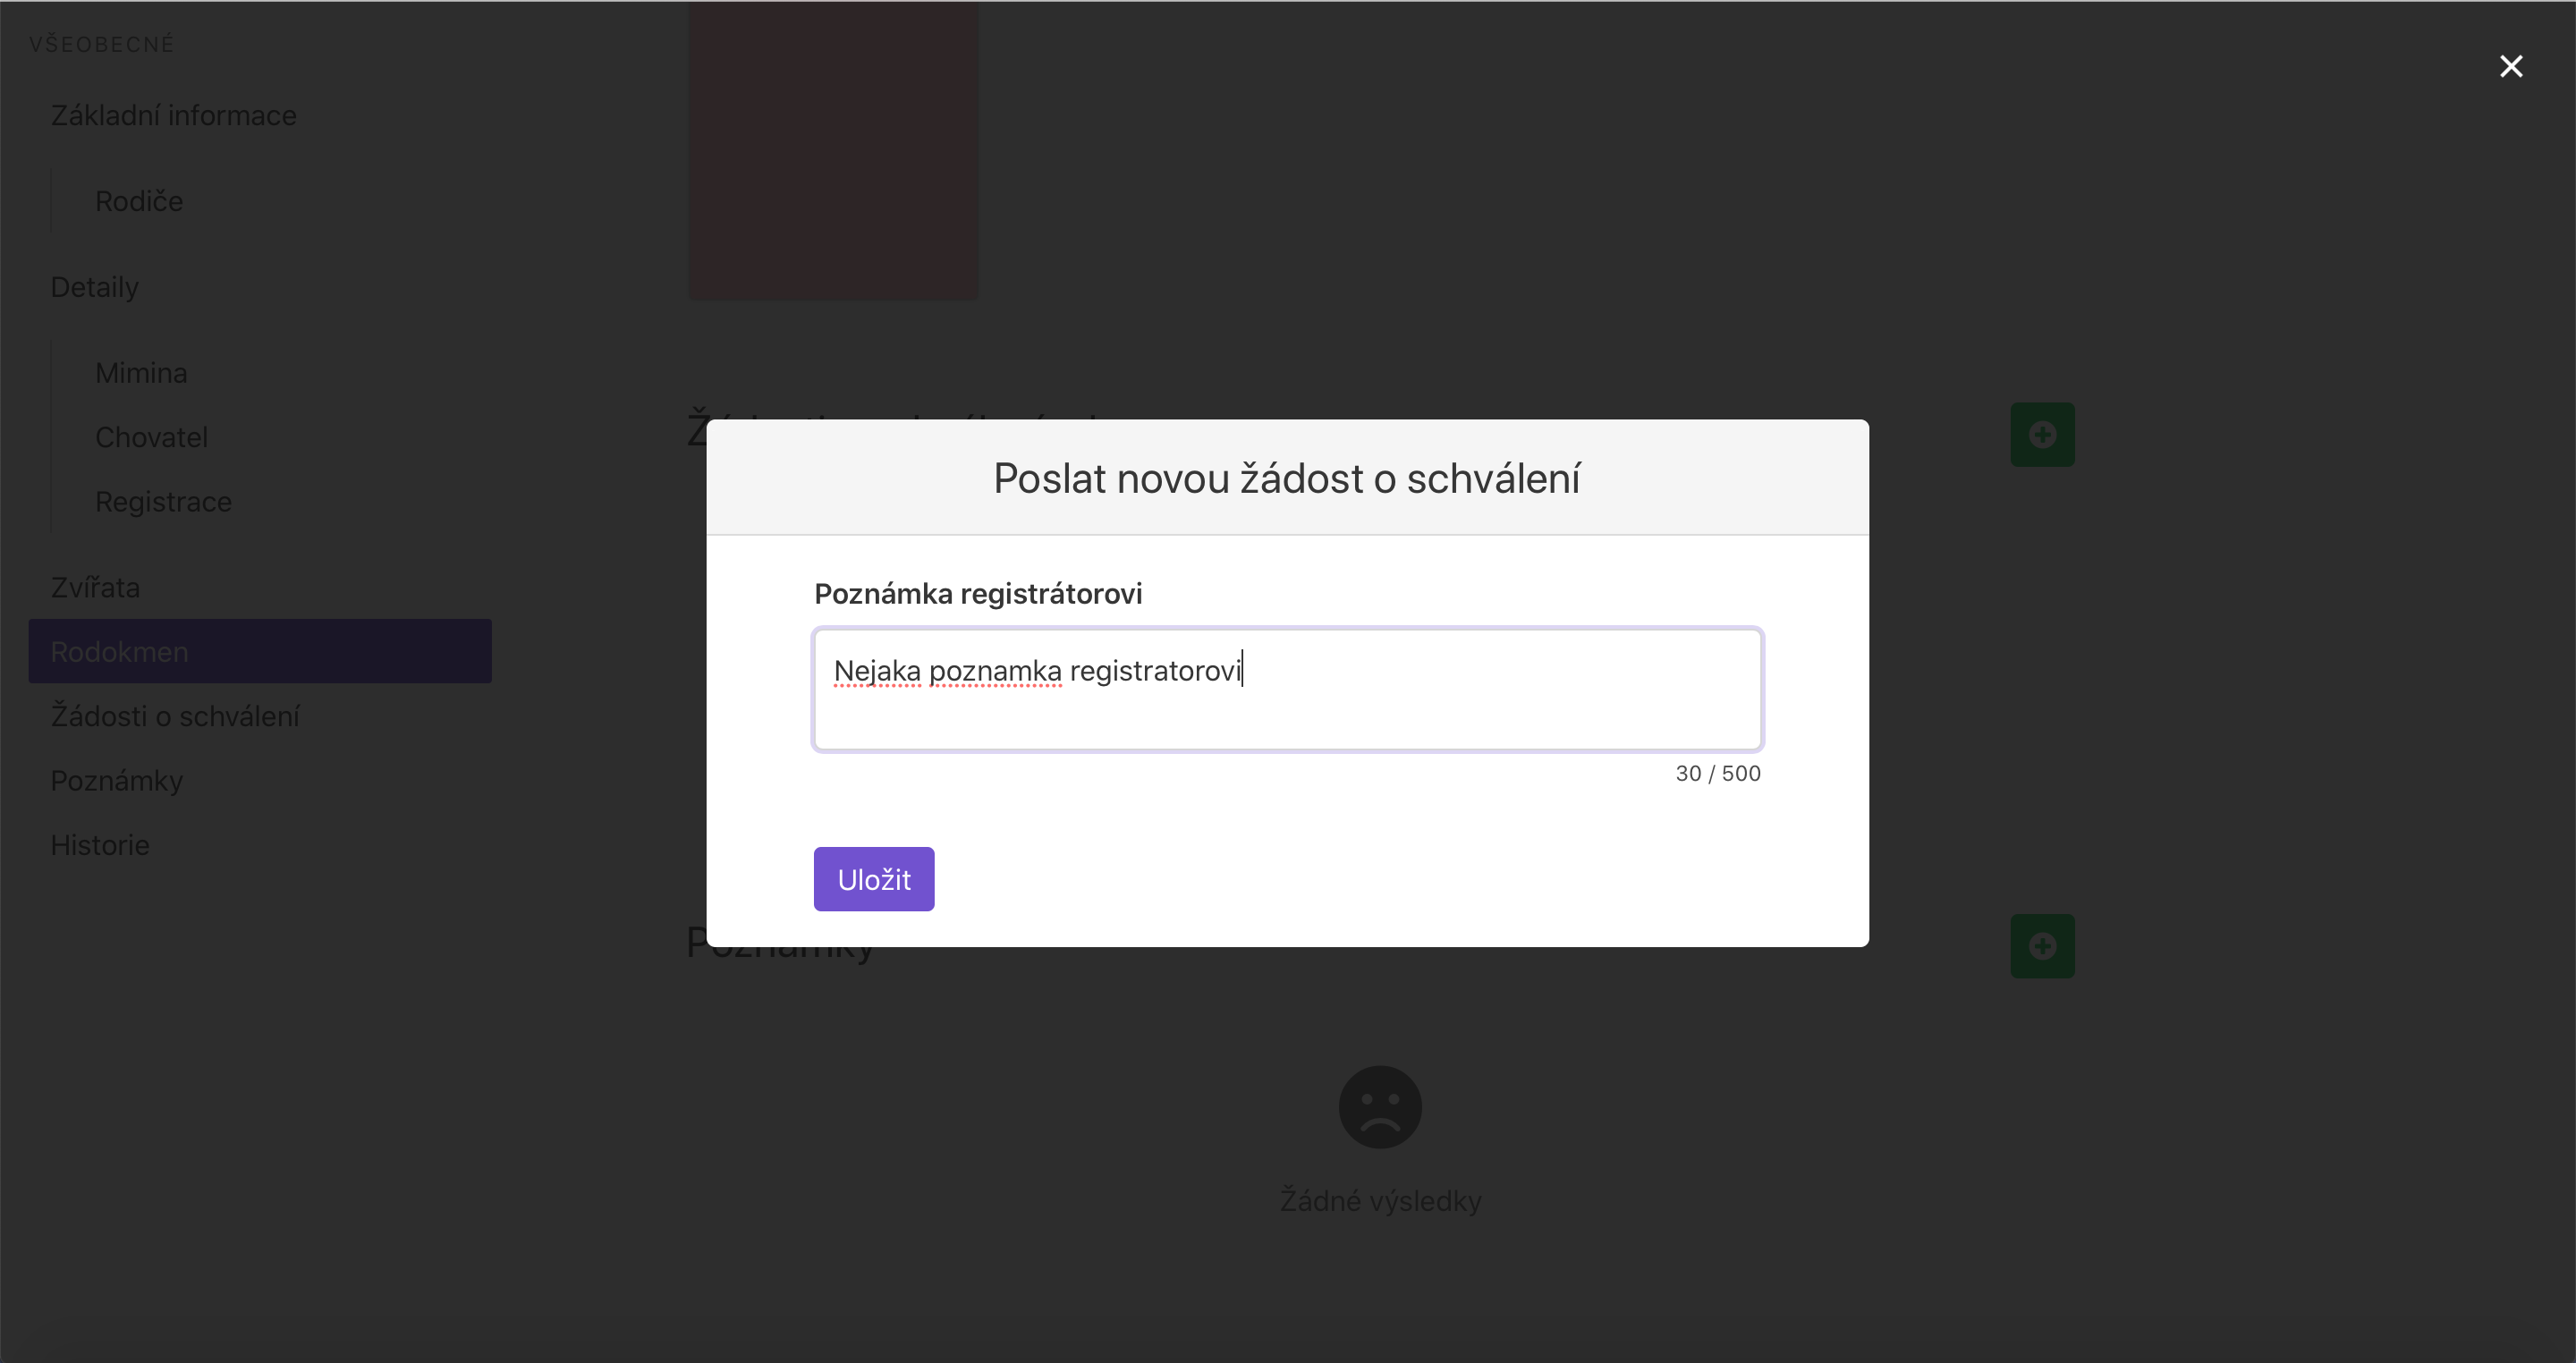
\includegraphics[width=1.0\textwidth]{media/priloha/vrh/ziadost/1.png}
	\caption{Screenshot aplikácie zobrazujúci modálne okno poslania žiadosti o schválenie vrhu}
\end{figure}

\begin{figure}[H]
	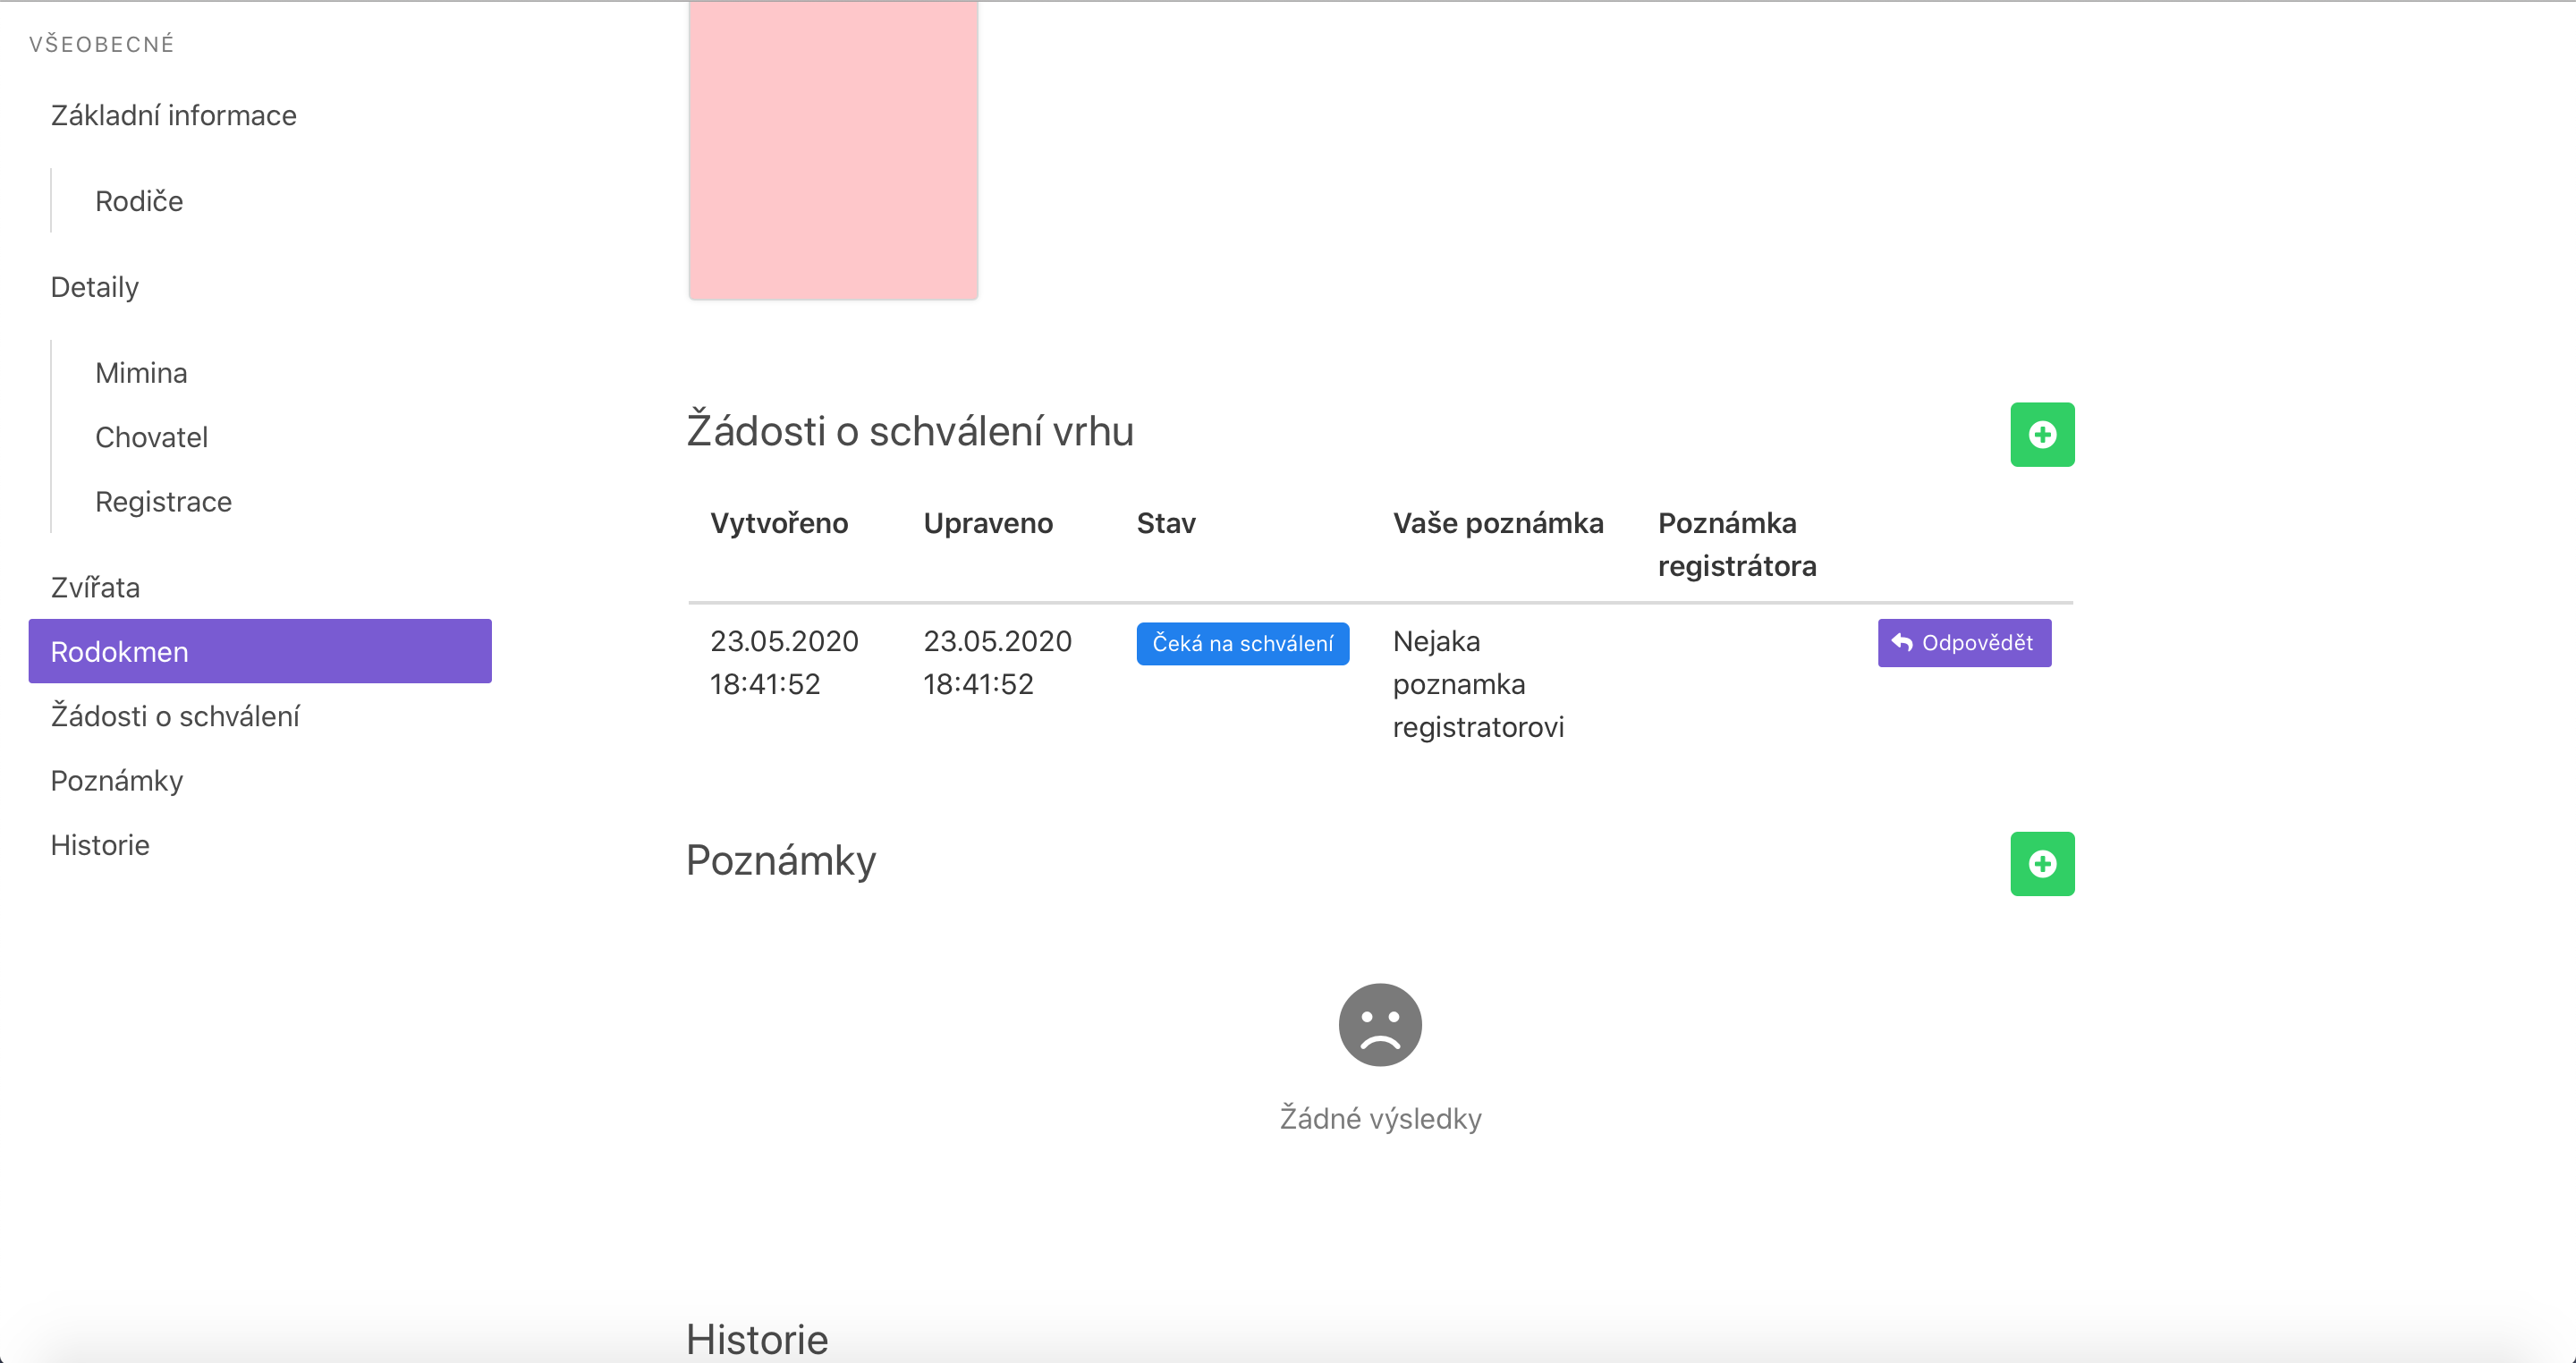
\includegraphics[width=1.0\textwidth]{media/priloha/vrh/ziadost/2.png}
	\caption{Screenshot aplikácie zobrazujúci poslanú žiadosť o schválenie vrhu}
\end{figure}

\vspace*{\fill}

\begin{figure}[H]
	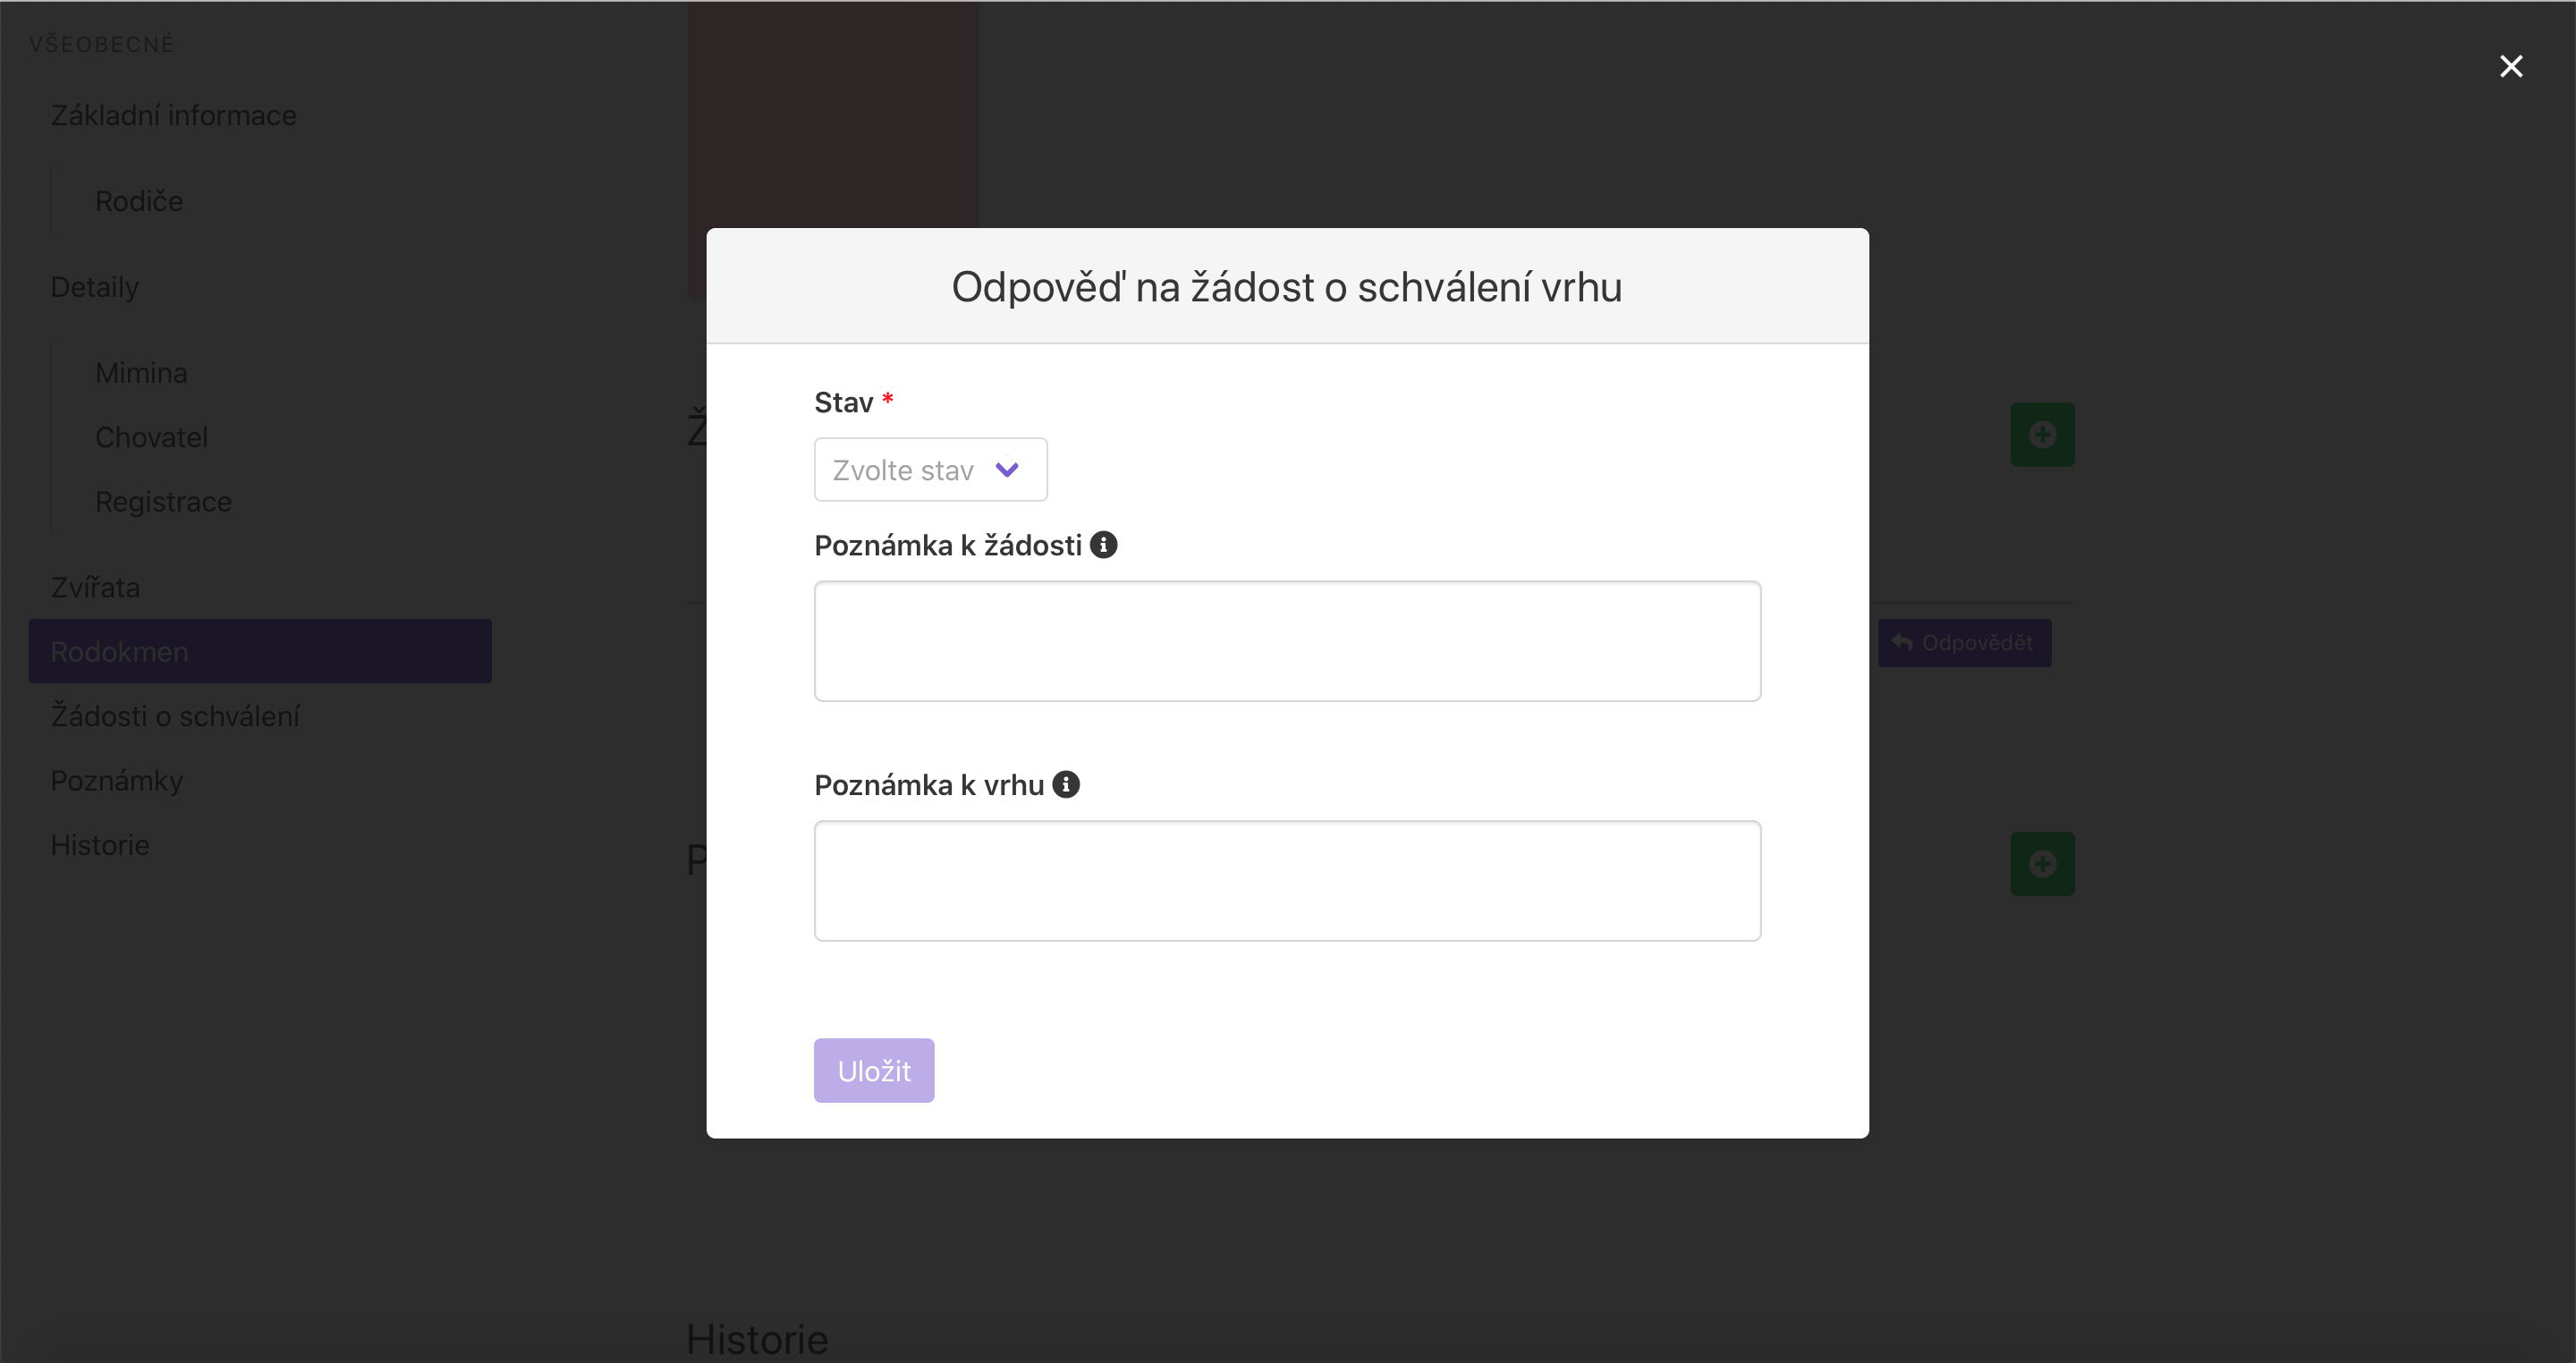
\includegraphics[width=1.0\textwidth]{media/priloha/vrh/ziadost/3.png}
	\caption{Screenshot aplikácie zobrazujúci modálne okno odpovedi na poslanú žiadosť}
\end{figure}

\begin{figure}[H]
	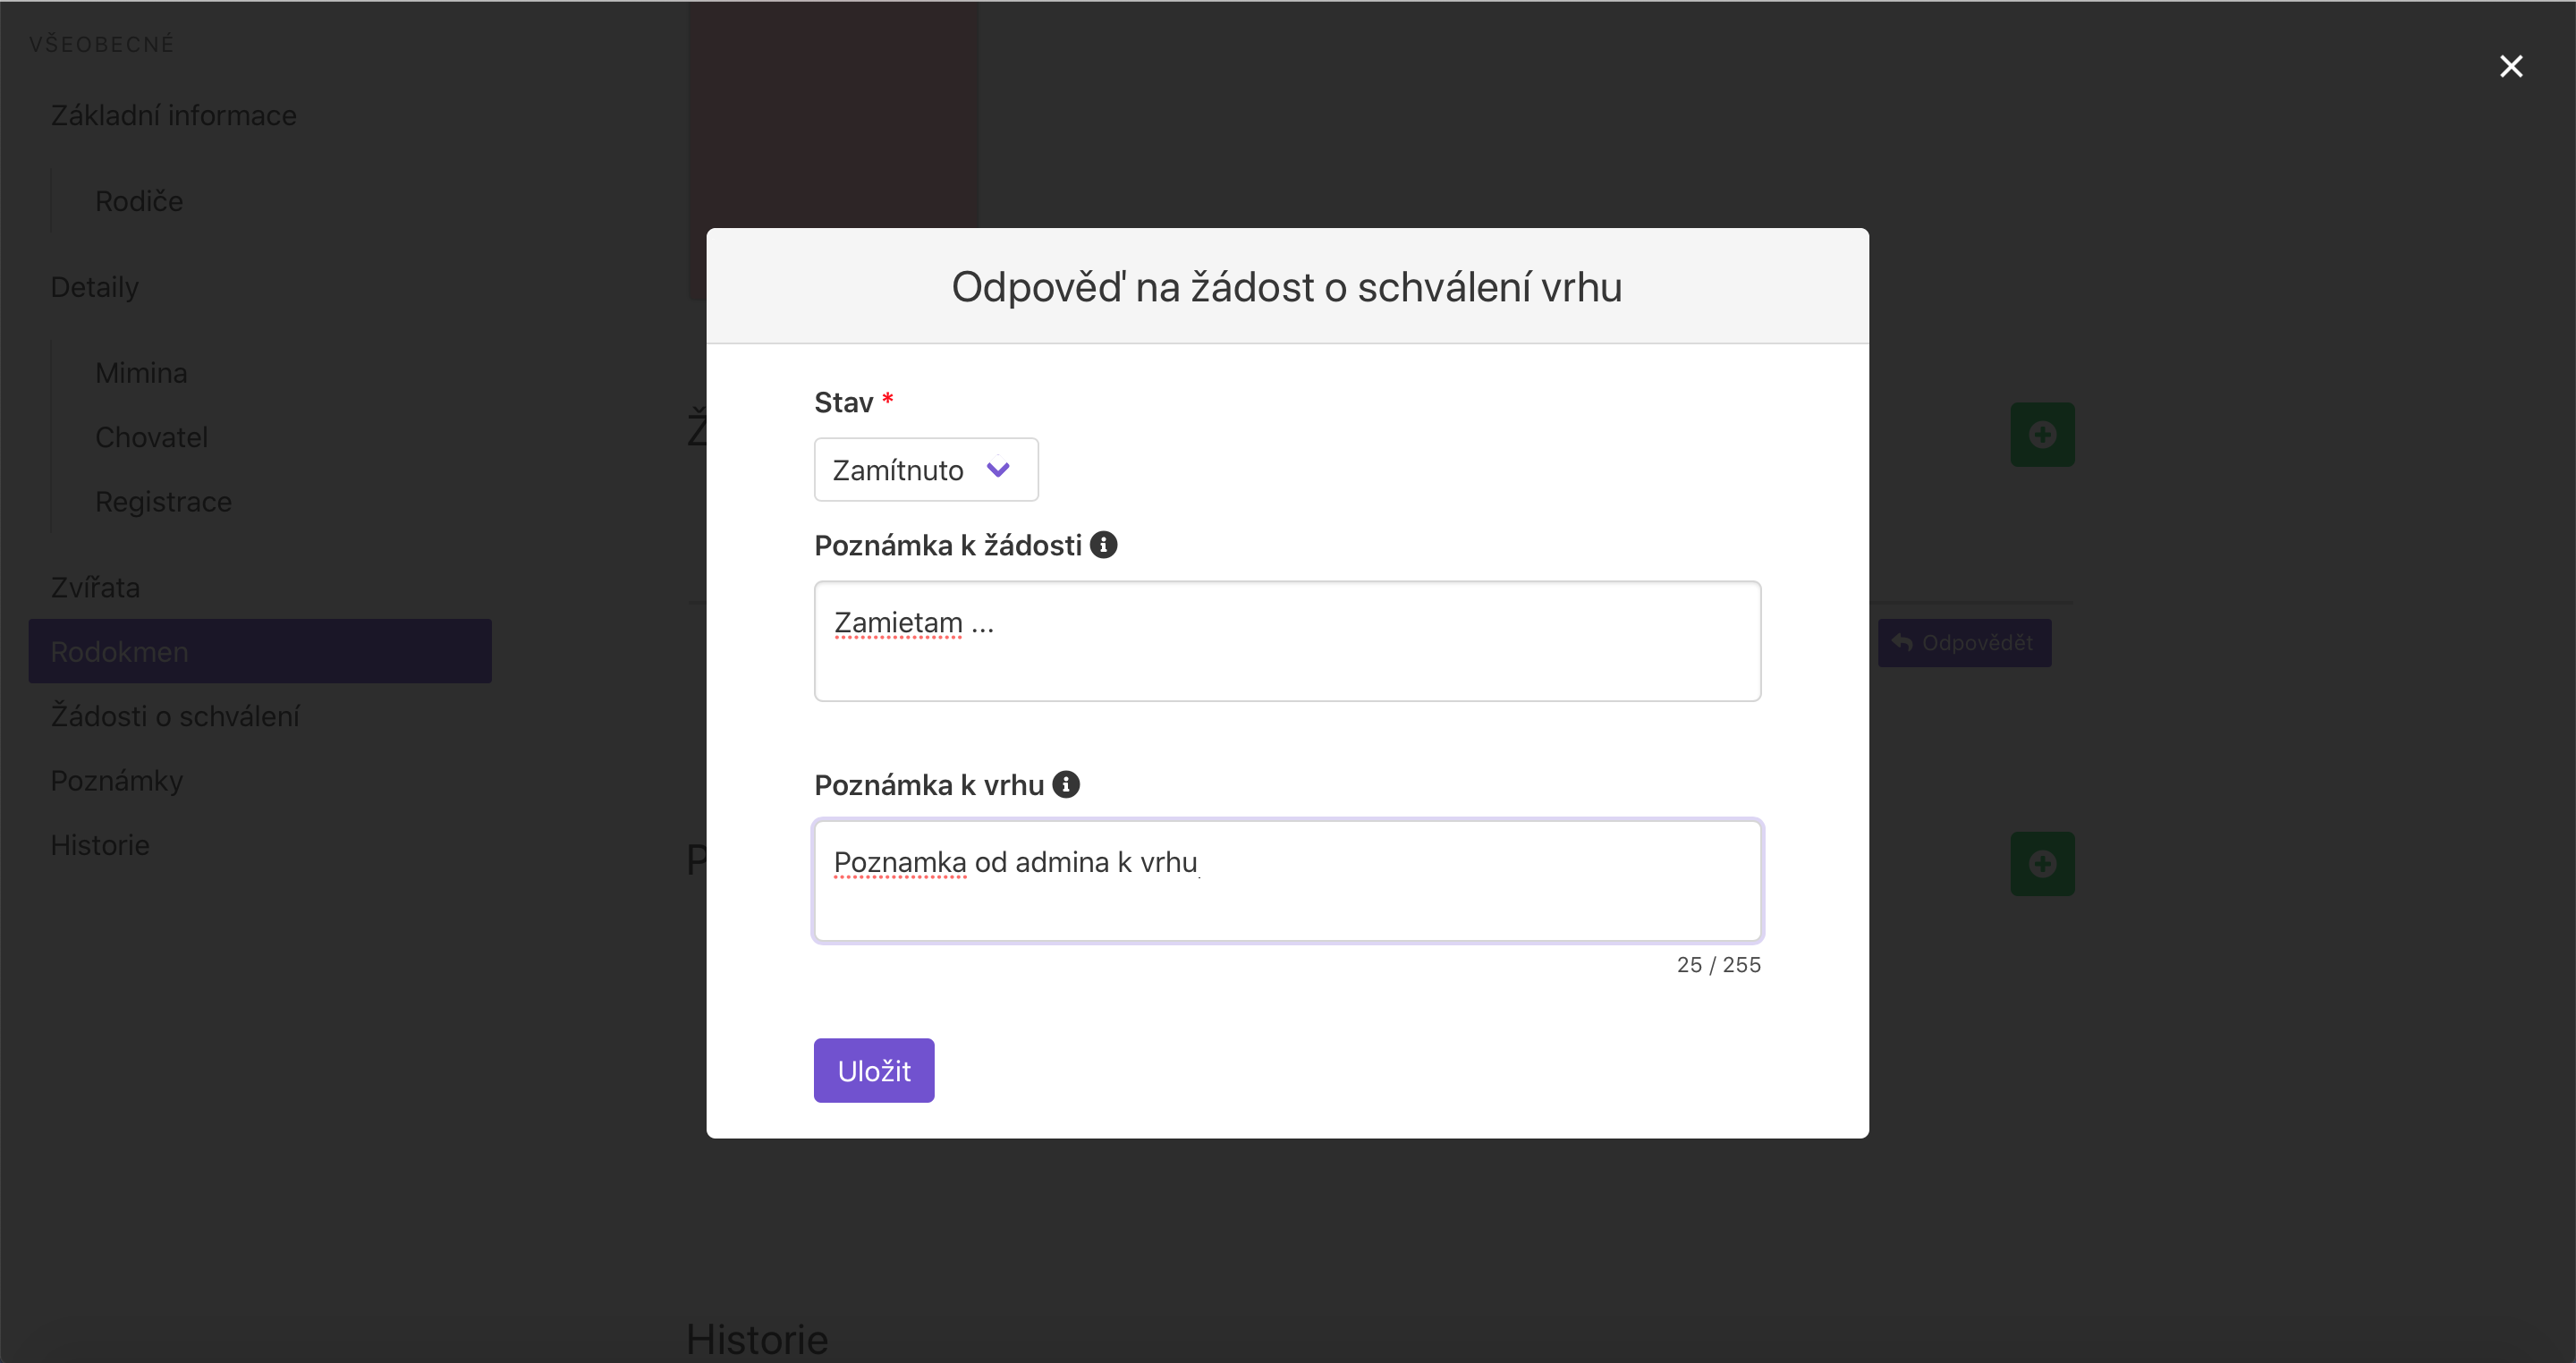
\includegraphics[width=1.0\textwidth]{media/priloha/vrh/ziadost/4.png}
	\caption{Screenshot aplikácie zobrazujúci modálne okno vyplnenej odpovedi na poslanú žiadosť}
\end{figure}

\vspace*{\fill}

\begin{figure}[H]
	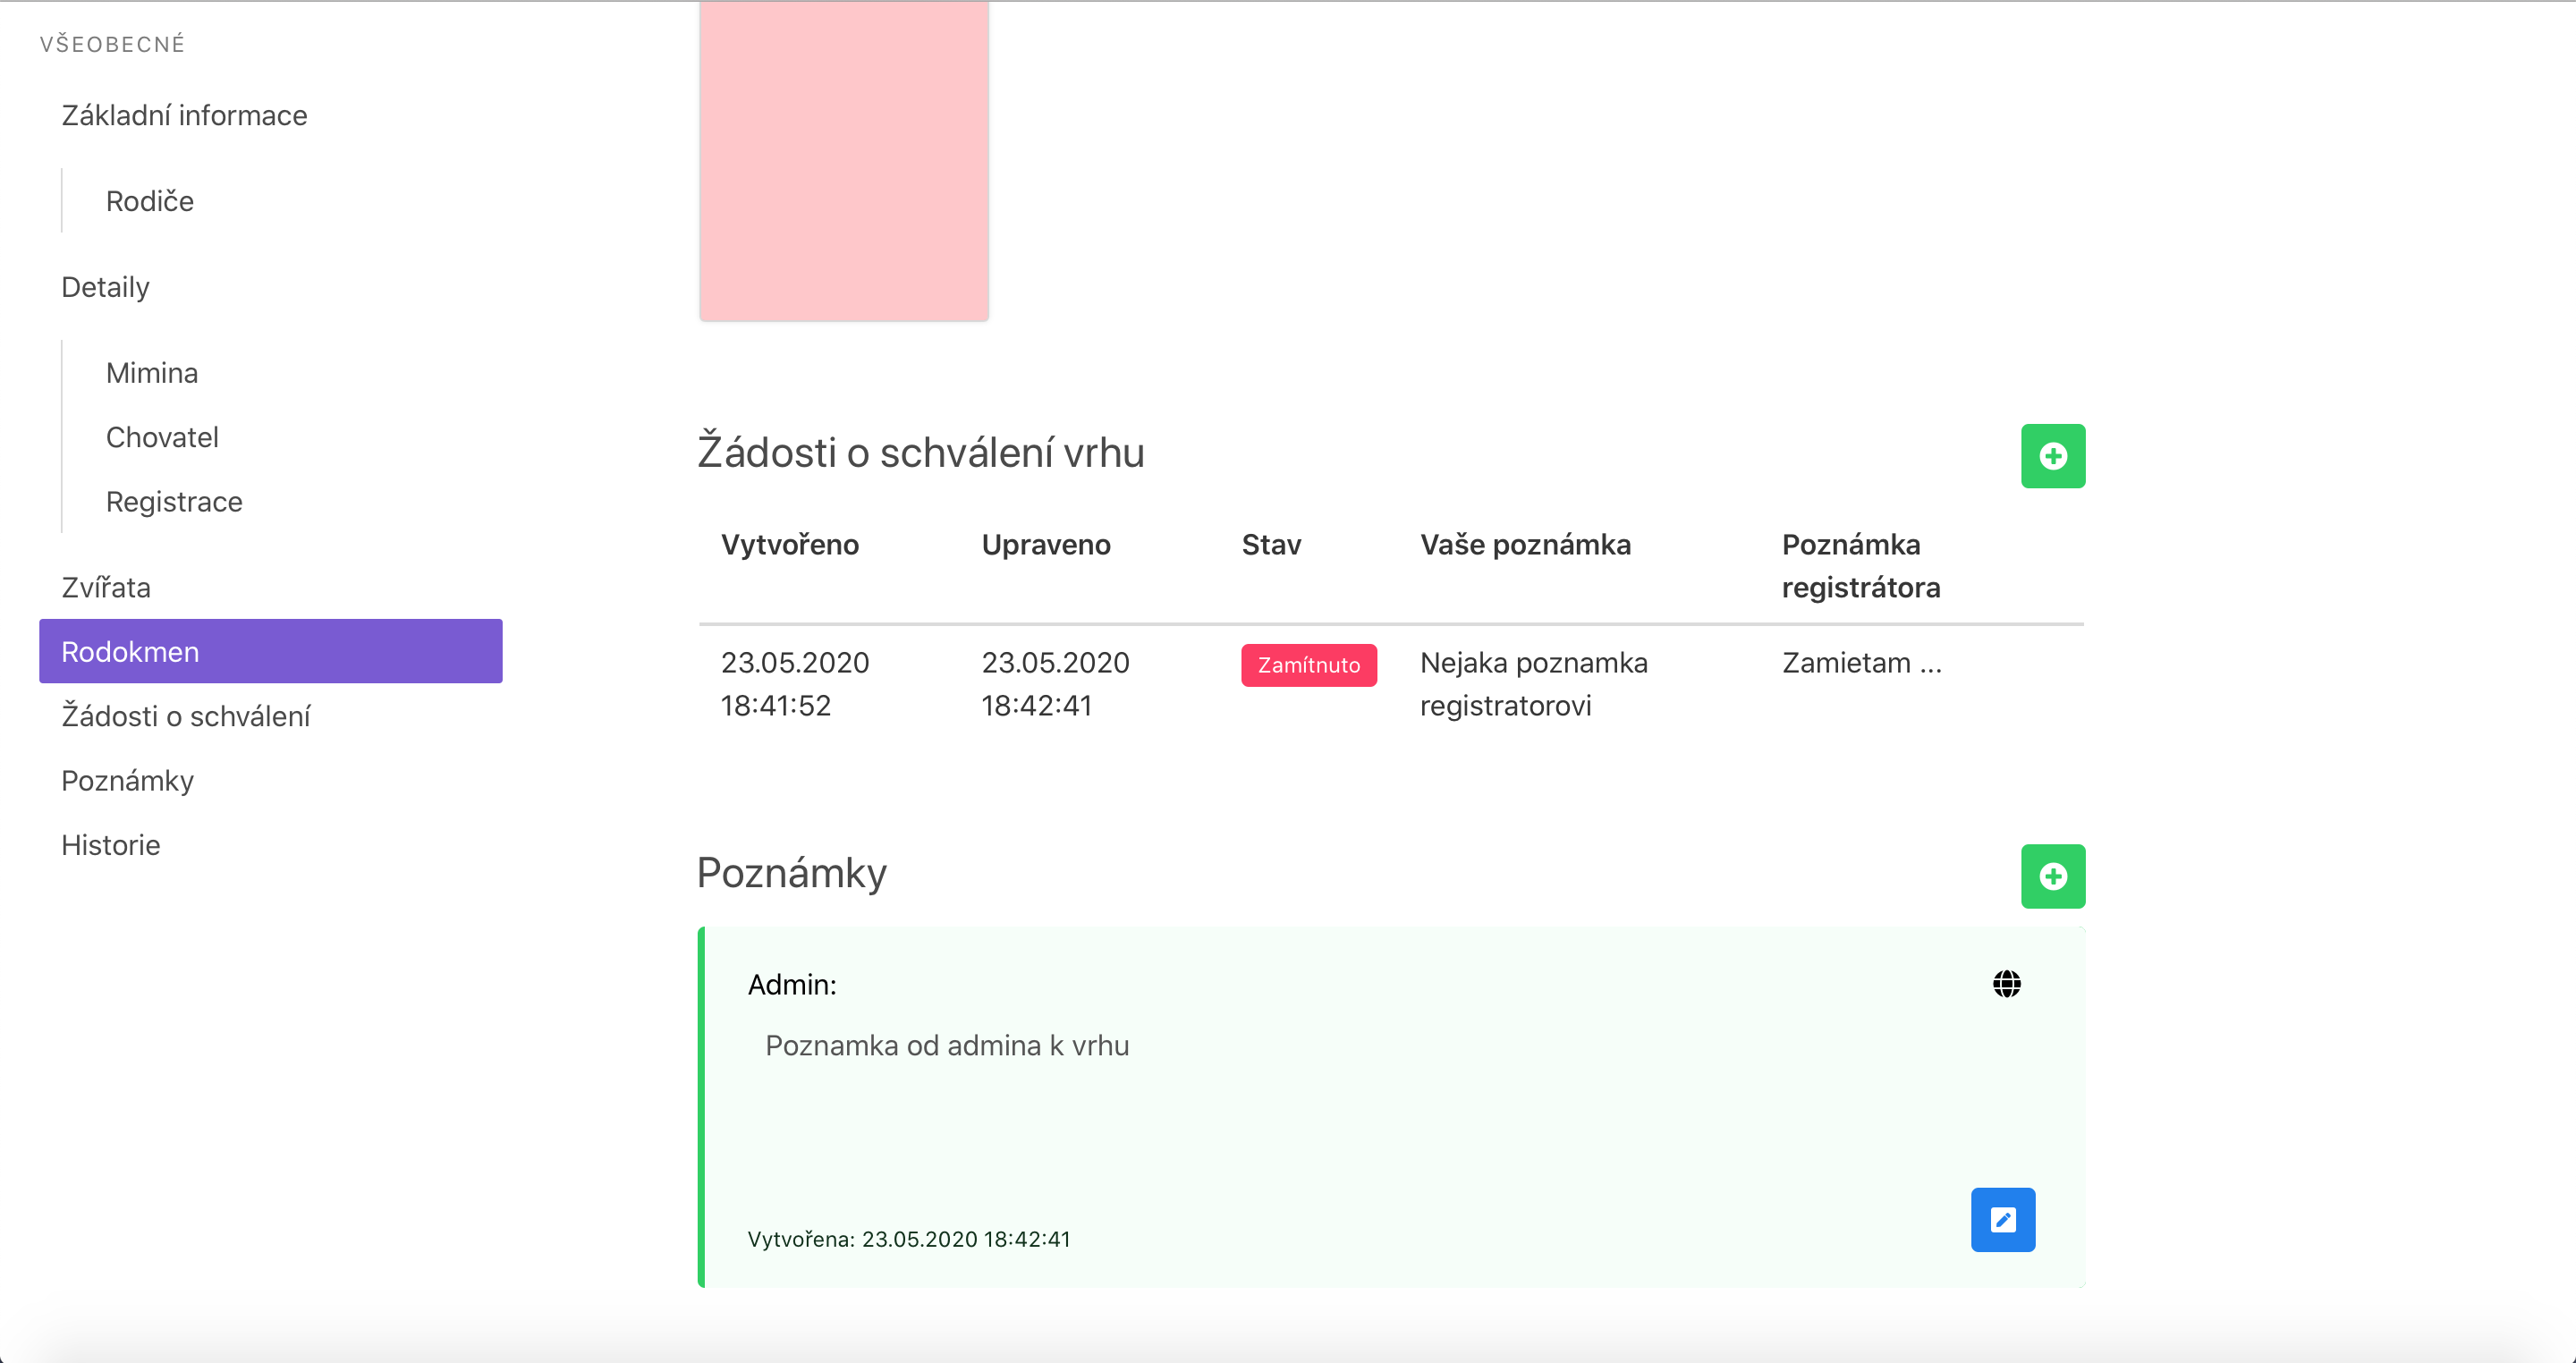
\includegraphics[width=1.0\textwidth]{media/priloha/vrh/ziadost/5.png}
	\caption{Screenshot aplikácie zobrazujúci zamietnutú žiadosť}
\end{figure}

\begin{figure}[H]
	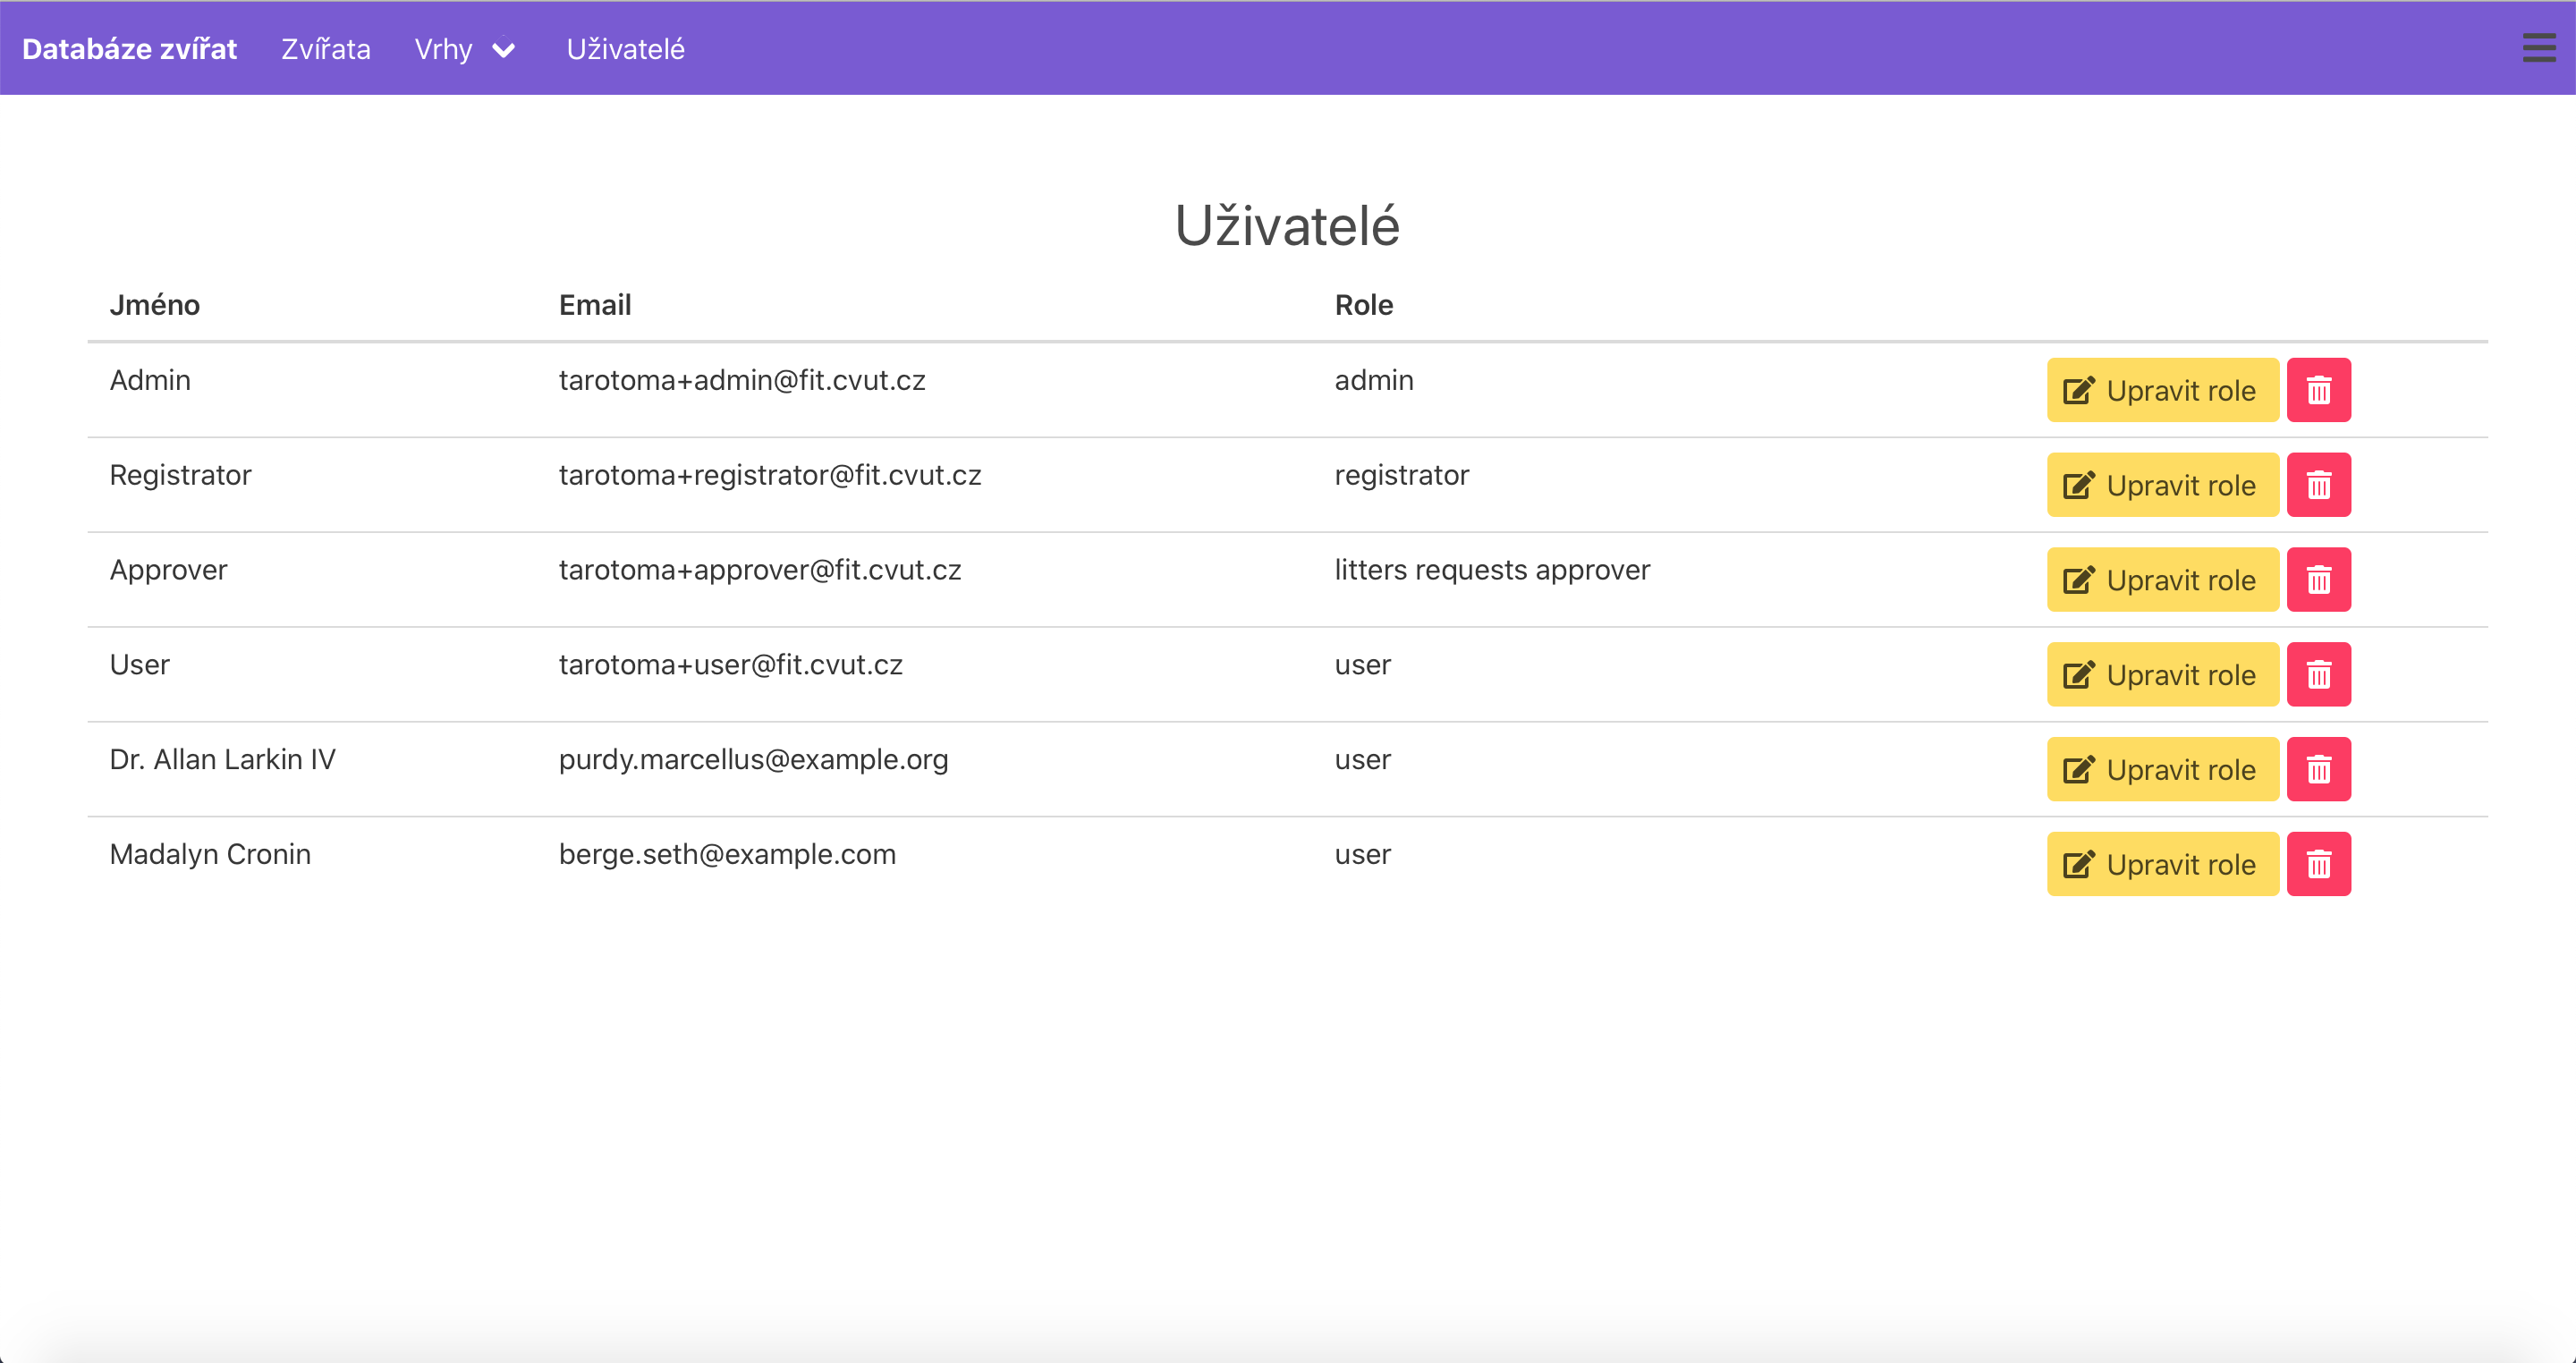
\includegraphics[width=1.0\textwidth]{media/priloha/pouzivatelia/1.png}
	\caption{Screenshot aplikácie zobrazujúci všetkých používateľov aplikácie}
\end{figure}

\vspace*{\fill}

\begin{figure}[H]
	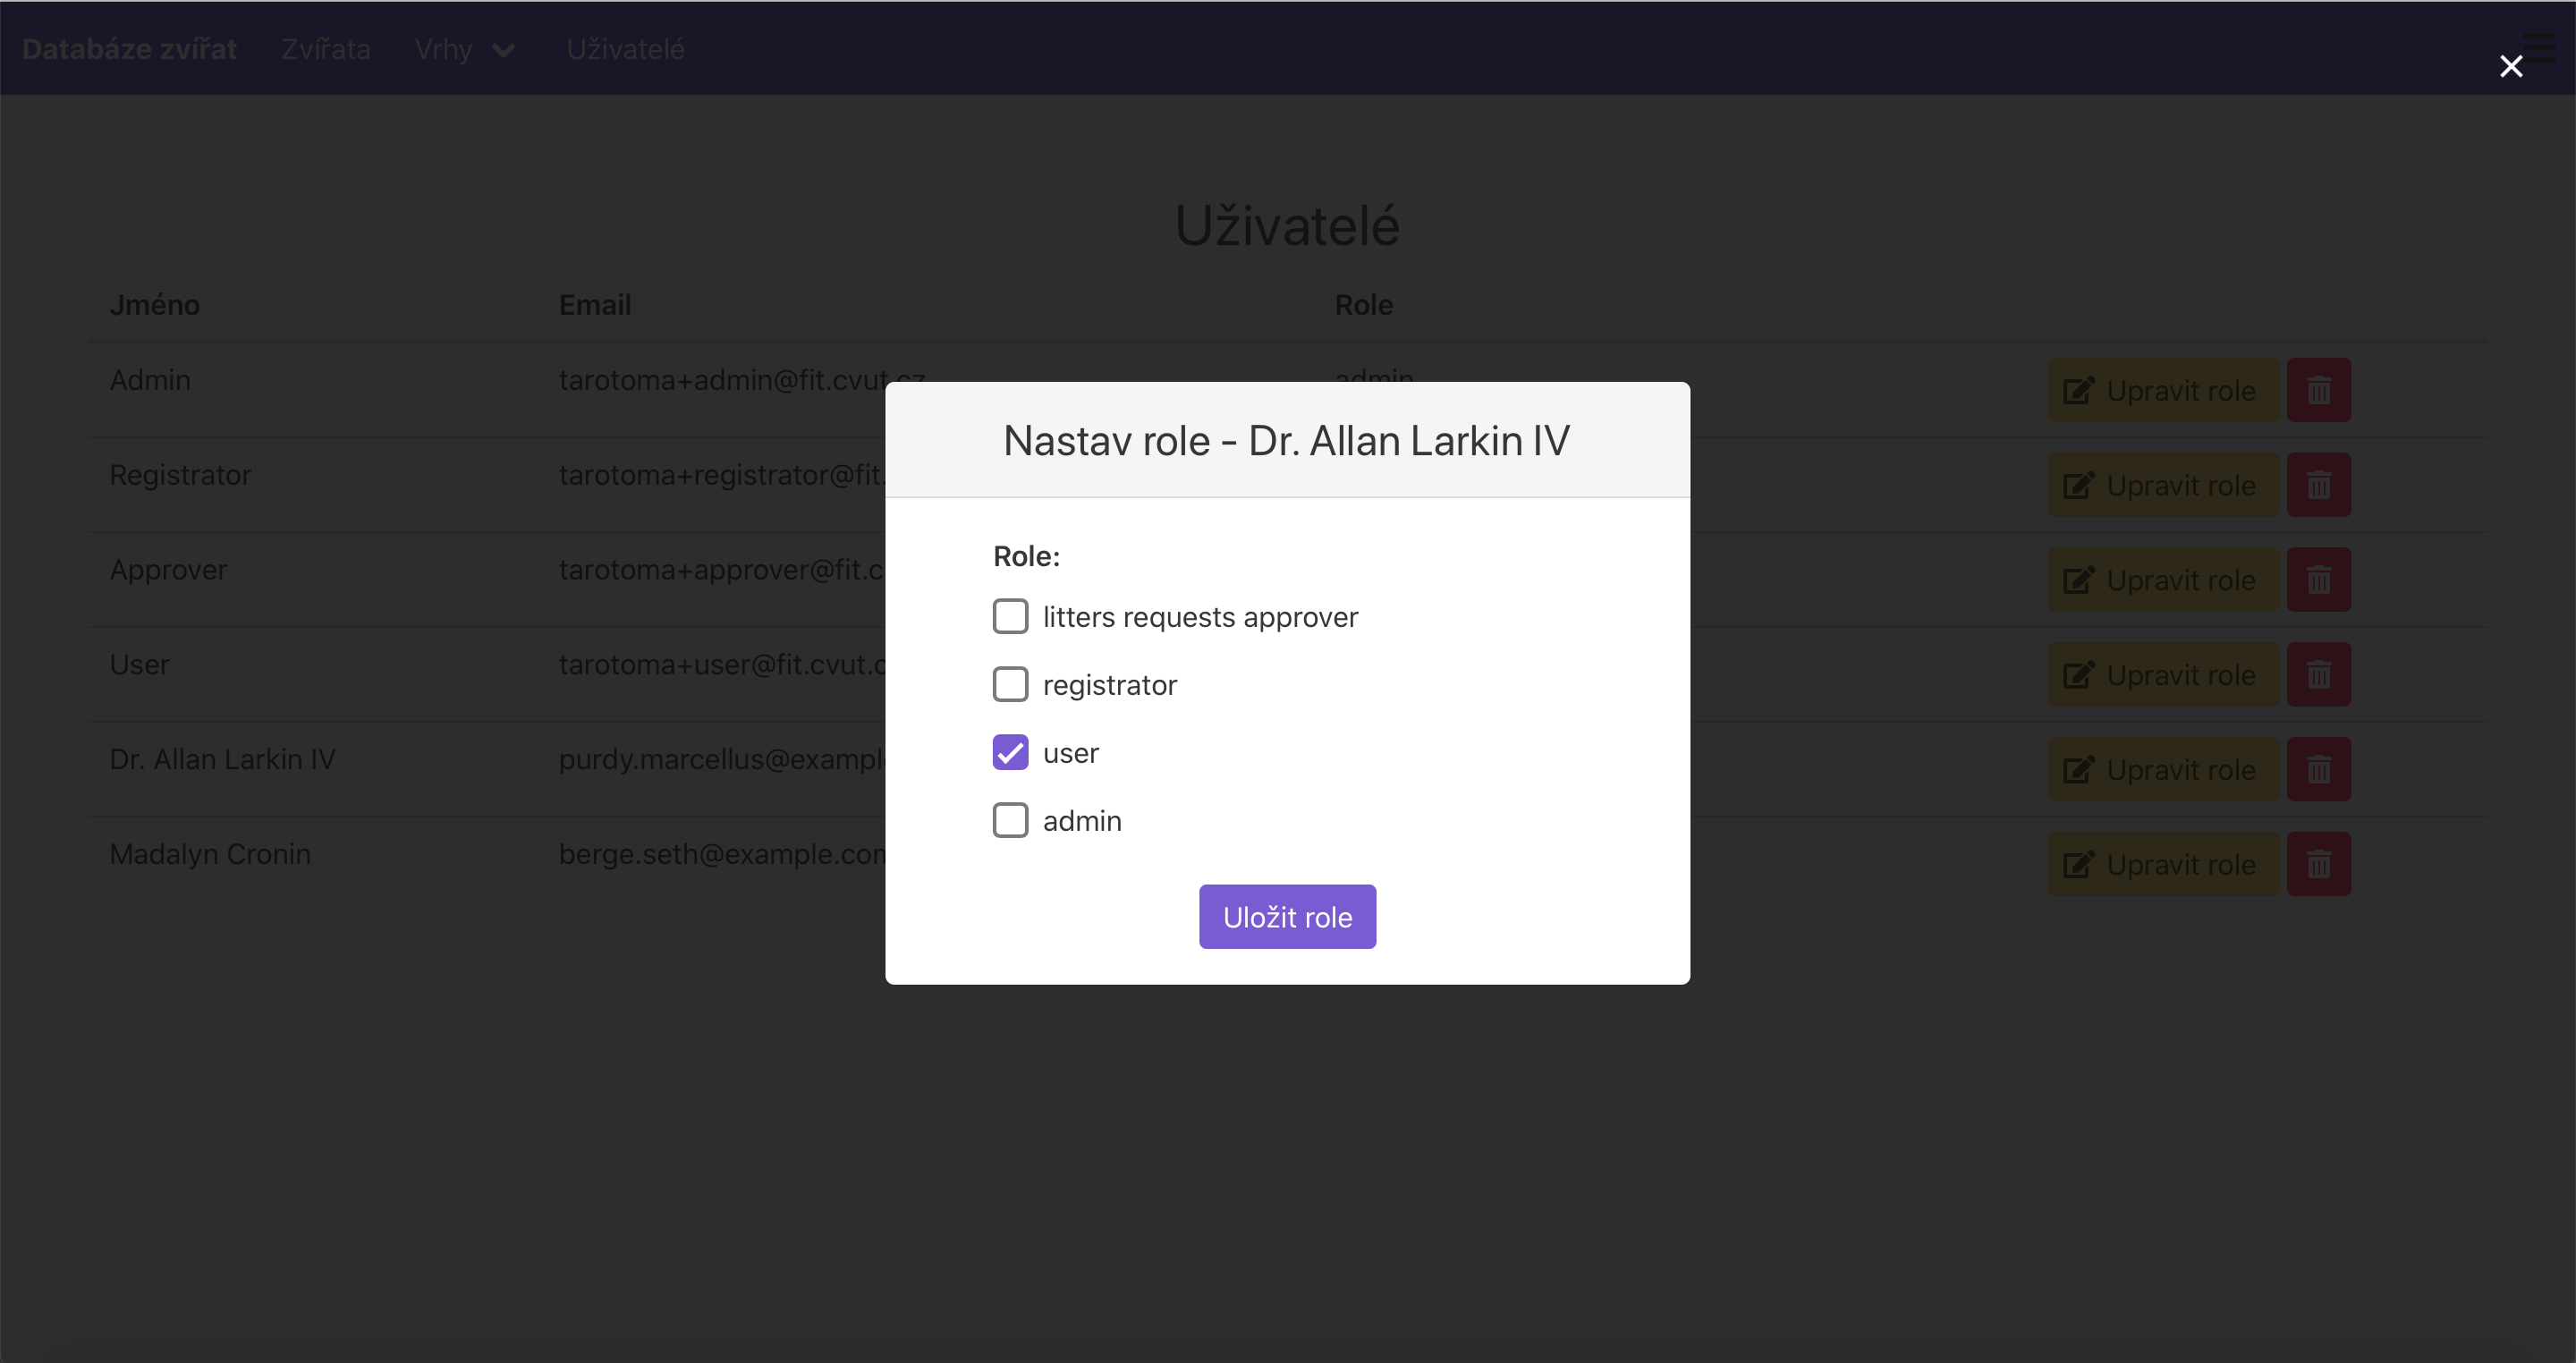
\includegraphics[width=1.0\textwidth]{media/priloha/pouzivatelia/2.png}
	\caption{Screenshot aplikácie zobrazujúci nastavenie rolí používateľovi aplikácie}
\end{figure}




